% -*- mode: noweb; noweb-default-code-mode: R-mode; -*-
\documentclass[a4paper]{book}
%\documentclass[envcountsame,envcountchap]{svmono}


\usepackage{graphicx,url}
\usepackage{amssymb}

\def\pf{{\bf Proof. }}
\def\logimplies{\Rightarrow}
\def\convinlaw{\stackrel{{\cal L}}{\Longrightarrow }}
\def\convinp{\stackrel{P}{\longrightarrow }}
\def\convas{\stackrel{a.s.}{\longrightarrow }}
\def\convv{\stackrel{v}{\longrightarrow}}
\def\asymp{\stackrel{{\mathbb P}}{\sim}}
\def\RR{\mathbb R}
\def\ZZ{\mathbb Z}
\def\QQ{\mathbb Q}
\def\NN{\mathbb N}
\def\MM{\mathbb M}
\def\LL{\mathbb L}
\def\EE{\mathbb E}
\def\PP{\mathbb P}
\def\DD{\mathbb D}
\def\WW{\mathbb W}
\def\FF{\mathbb F}
\def\II{\mathbb I}
\def\FF{\mathbb F}
\def\XX{\mathbb X}
\def\sige{\sigma_{\epsilon}}

\def\eqinlaw{\stackrel{{\cal L}}{=}}
\def\tends{\rightarrow}
\def\tendsinf{\rightarrow\infty}
\def\isodynamo{\Leftrightarrow}

\newtheorem{Theorem}{Theorem}
\newtheorem{Lemma}{Lemma}
\newtheorem{Corollary}{Corollary}
\newtheorem{Proposition}{Proposition}
\newtheorem{Definition}{Definition}
\newtheorem{Remark}{Remark}
\newcommand{\mbf}[1]{\mbox{\boldmath $#1$}}

\setlength{\textwidth}{6.5in} \setlength{\textheight}{9in}
\setlength{\evensidemargin}{12pt} \setlength{\oddsidemargin}{0in}
\setlength{\topmargin}{1in}
\renewcommand{\baselinestretch}{1.3}
\setlength{\headheight}{0.2in} 
\setlength{\headsep}{0.2in}

%- Makes the section title start with Appendix in the appendix environment
\newcommand{\Appendix}
{%\appendix
%\def\thesection{Appendix~\Alph{section}}
\def\thesection{Appendix~\Alph{chapter}}
%\def\thesubsection{\Alph{section}.\arabic{subsection}}
%\def\thesubsection{A.\arabic{subsection}}
\def\thesubsection{A.\arabic{section}}
}


%\pagestyle{empty}
\usepackage{amssymb}
\usepackage{amsmath}
\usepackage{latexsym}
\usepackage{epsfig}
%\usepackage{html}
\usepackage{verbatim}
\usepackage{hyperref}
\usepackage{float}
\usepackage[utf8]{inputenc}
\usepackage{a4wide}

\title{Multivariate Direct Filter Approach (MDFA)}
\author{Marc Wildi and Tucker McElroy}




\usepackage{Sweave}
\begin{document}

\maketitle

\date{}

%\SweaveOpts{prefix.string=c:/wia/tmp/bar}

\frontmatter%%%%%%%%%%%%%%%%%%%%%%%%%%%%%%%%%%%%%%%%%%%%%%%%%%%%%%

%\include{dedic}
%\newpage
%\phantom{rete}
%\newpage
%\include{preface}




\tableofcontents


\mainmatter%%%%%%%%%%%%%%%%%%%%%%%%%%%%%%%%%%%%%%%%%%%%%%%%%%%%%%%

%-----------------------------------------------

% Parallelized computation chapters customization and replication
% simanz<-100 chapters customization and replication
% Load all chapters

\chapter{Introduction}\label{intro_sec}

\section{Classic Model-Based Paradigm}

Marc's perspective:
\begin{itemize}
\item Maximum Likelihood, main purpose: determine DGP. If DGP is known then optimality can be invoked, in principle. 
\item Problem: model misspecification. Pseudo maximum likelihood: one-step ahead mean-square criterion. 
\item Emphasizes short-term performances, only (contrast with real-time trend extraction: long-term component). 
\item Rigid criterion: can account neither for relevant problem-structure (signal extraction=one and multi-step ahead forecasts) nor for various user-priorities (ATS-trilemma).
\end{itemize}

Tucker/Chris' perspectives:...


\section{A Shift of Perspective: Tackling the (Relevant) Problem-Structure and Addressing User-Priorities}

Refer to DFA and Trilemma papers with Tucker. Refer to chapters \ref{mse_sec} (problem structure) and \ref{ats_sec} (user-priorities). 

\section{Univariate DFA}

Refer to DFA-paper with Tucker and \href{http://blog.zhaw.ch/sef/files/2014/10/DFA.pdf}{DFA} (Sweave environment: replication). 


\section{This Book's Contribution: Multivariate (M-) DFA}

Problem structure (chapter \ref{mse_sec}); forecasting/nowcasting/backcasting and filter revisions (chapter \ref{fil_sec});filter constraints (chapter \ref{con_sec}); ATS-trilemma, customization and user-priorities (chapter \ref{ats_sec}); replicating and enhancing classical model-based approaches and HP/CF-filters (chapter \ref{rep_sec}); addressing more sophisticated gain/loss structures (chapter \ref{exo_sec}); developing inferential aspects (chapter \ref{inf_sec}); Regularization Troika and tackling overfitting (chapter \ref{reg_sec}); data-revisions (chapter \ref{rev_sec}); solving the mixed-frequency problem (chapter \ref{mix_sec}); extensions to non-stationary integrated (chapter \ref{int_sec}) and cointegrated processes (chapter \ref{coint_sec}); adaptive filtering (chapter \ref{ada_sec}).




\section{R-Code}

We here briefly review the main R-code files and provide support for installation.

\subsection{Getting Started: Setting the Paths}

Start from a clean-sheet when replicating results in this book:
\begin{Schunk}
\begin{Sinput}
> rm(list=ls())
\end{Sinput}
\end{Schunk}
The R-code in the various chapters of this book requires installation of the following R-packages:
\begin{Schunk}
\begin{Sinput}
> # Load packages: time series and xts
> library(tseries)
> library(xts)
> # State-space models (will be replicated by MDFA) 
> library(dlm)
> # Numerical package 
> library(numDeriv)
> # Graphical package for recession-shading (empirical examples based on US-GDP)
> library(tis) 
> #install.packages("devtools")
> library(devtools)
> # Load MDFA package from github
> devtools::install_github("wiaidp/MDFA")
> # MDFA package
> library(MDFA) 
\end{Sinput}
\end{Schunk}
US-GDP data for the empirical examples can be retrieved either directly from Quandl (this would require preliminary user-registration, though) or from a local data-folder which is the default-setting:
\begin{Schunk}
\begin{Sinput}
> # Load fresh data from quandl: T/F
> #   Default-setting is False: the data will be loaded from local data folder
> load_from_quandl<-F
\end{Sinput}
\end{Schunk}
Paths to MDFA-code as well as to the (US-GDP) data must be provided. It is assumed that the MDFA-package is saved to a main folder containing DFA-, MDFA-, model-based- and data-subfolders. The R-code in the book generates pdf-graphs which are saved in a separate folder whose path is specified by path.out.
\begin{Schunk}
\begin{Sinput}
> # Specify disk
> disk_id<-"C"
> # Set main path
> path.main<-paste(disk_id,
+       ":\\wia_desktop\\Projekte\\2016\\MDFA-Legacy\\Sweave\\",sep="")
> # Set paths to subfolders
>   # Path to Latex-folder: all pdfs generated by the R-code are filed there
> path.out<-paste(path.main,"Latex\\",sep="")
>   # Path to data (US-GDP)
> path.dat<-paste(path.main,"Data\\",sep="")
>   # Path to code that is part of MDFA-Legacy project but not part of MDFA-package 
> path.pgm<-paste(path.main,"R\\",sep="")
\end{Sinput}
\end{Schunk}
The (univariate) DFA-code is the same as in \href{http://blog.zhaw.ch/sef/files/2014/10/DFA.pdf}{DFA}: all  empirical examples are and will be fully compatible. 

\subsection{DFA}\label{dfa_intro}
We here briefly review the relevant \href{http://blog.zhaw.ch/sef/files/2014/10/DFA.pdf}{DFA}\footnote{Left-click to activate the hyperlink.}-pieces (anchoring). 

\subsubsection{DFT and Periodogram}

The Discrete Fourier Transform (DFT) and the periodogram are defined in \href{http://blog.zhaw.ch/sef/files/2014/10/DFA.pdf}{DFA}, sections 2.2 and 2.3. The following per(iodogram) function in the MDFA-package replicates these formulae\footnote{Note that frequency $\pi$ is treated differently, whether the sample size is odd or even, and that frequency zero is scaled by $1/\sqrt{2}$ which will be explained later on.}.  
\begin{Schunk}
\begin{Sinput}
> head(per,100)
\end{Sinput}
\begin{Soutput}
1  function (x, plot_T)                                                              
2  {                                                                                 
3      len <- length(x)                                                              
4      per <- 0:(len/2)                                                              
5      DFT <- per                                                                    
6      for (k in 0:(len/2)) {                                                        
7          cexp <- exp(-(0+1i) * (1:len) * 2 * pi * k/len)                           
8          DFT[k + 1] <- sum(cexp * x * sqrt(1/(2 * pi * len)))                      
9      }                                                                             
10     DFT[1] <- DFT[1]/sqrt(2)                                                      
11     if (abs(as.integer(len/2) - len/2) < 0.1)                                     
12         DFT[k + 1] <- DFT[k + 1]/sqrt(2)                                          
13     per <- abs(DFT)^2                                                             
14     if (plot_T) {                                                                 
15         par(mfrow = c(2, 1))                                                      
16         plot(per, type = "l", axes = F, xlab = "Frequency", ylab = "Periodogram", 
17             main = "Periodogram")                                                 
18         axis(1, at = 1 + 0:6 * len/12, labels = c("0", "pi/6",                    
19             "2pi/6", "3pi/6", "4pi/6", "5pi/6", "pi"))                            
20         axis(2)                                                                   
21         box()                                                                     
22         plot(log(per), type = "l", axes = F, xlab = "Frequency",                  
23             ylab = "Log-periodogram", main = "Log-periodogram")                   
24         axis(1, at = 1 + 0:6 * len/12, labels = c("0", "pi/6",                    
25             "2pi/6", "3pi/6", "4pi/6", "5pi/6", "pi"))                            
26         axis(2)                                                                   
27         box()                                                                     
28     }                                                                             
29     return(list(DFT = DFT, per = per))                                            
30 }                                                                                 
\end{Soutput}
\end{Schunk}
This function will be generalized in the new multivariate setting.

\subsubsection{DFA: Mean-Square Perspective}

A simple MSE (Mean-Square Error) version of the DFA, as proposed in \href{http://blog.zhaw.ch/sef/files/2014/10/DFA.pdf}{DFA}, section 4.1, is included in the MDFA-package:  

\begin{Schunk}
\begin{Sinput}
> # This function computes mean-square DFA-solutions
> # L is the length of the MA filter,
> # periodogram is the frequency weighting function in the DFA
> # Gamma is the transferfunction of the symmetric filter (target) and
> # Lag is the lag-parameter: Lag=0 implies real-time filtering, Lag=L/2
> #     implies symmetric filter
> # The function returns optimal coefficients as well as the transfer 
> #     function of the optimized real-time filter
> head(dfa_ms,100)
\end{Sinput}
\begin{Soutput}
1  function (L, periodogram, Lag, Gamma)                                    
2  {                                                                        
3      K <- length(periodogram) - 1                                         
4      X <- exp(-(0+1i) * Lag * pi * (0:(K))/(K)) * rep(1, K + 1) *         
5          sqrt(periodogram)                                                
6      X_y <- exp(-(0+1i) * Lag * pi * (0:(K))/(K)) * rep(1, K +            
7          1)                                                               
8      for (l in 2:L) {                                                     
9          X <- cbind(X, (cos((l - 1 - Lag) * pi * (0:(K))/(K)) +           
10             (0+1i) * sin((l - 1 - Lag) * pi * (0:(K))/(K))) *            
11             sqrt(periodogram))                                           
12         X_y <- cbind(X_y, (cos((l - 1 - Lag) * pi * (0:(K))/(K)) +       
13             (0+1i) * sin((l - 1 - Lag) * pi * (0:(K))/(K))))             
14     }                                                                    
15     xtx <- t(Re(X)) %*% Re(X) + t(Im(X)) %*% Im(X)                       
16     b <- as.vector(solve(xtx) %*% (t(Re(X_y)) %*% (Gamma * periodogram)))
17     trffkt <- 1:(K + 1)                                                  
18     trffkt[1] <- sum(b)                                                  
19     for (k in 1:(K)) {                                                   
20         trffkt[k + 1] <- (b %*% exp((0+1i) * k * (0:(length(b) -         
21             1)) * pi/(K)))                                               
22     }                                                                    
23     return(list(b = b, trffkt = trffkt))                                 
24 }                                                                        
\end{Soutput}
\end{Schunk}
This function is nested in the multivariate MDFA in the sense that the latter can replicate the former perfectly when suitably parametrized, see section \ref{ex_rep_dfa}. 



\subsubsection{DFA: ATS-Trilemma and Customization}

A more general DFA-function, called \emph{dfa\textunderscore analytic}, is proposed in \href{http://blog.zhaw.ch/sef/files/2014/10/DFA.pdf}{DFA}, section 4.3.5. Customization and the generic ATS-trilemma are presented in \href{http://blog.zhaw.ch/sef/files/2014/10/DFA.pdf}{DFA}, sections 4.3 and 5. This function is included in the MDFA-package: 
\begin{Schunk}
\begin{Sinput}
> head(dfa_analytic)
\end{Sinput}
\begin{Soutput}
1 function (L, lambda, periodogram, Lag, Gamma, eta, cutoff, i1, 
2     i2)                                                        
3 {                                                              
4     lambda <- abs(lambda)                                      
5     eta <- abs(eta)                                            
6     K <- length(periodogram) - 1                               
\end{Soutput}
\end{Schunk}
The additional control parameters $lambda,eta$ allow for customization of the filter, see chapter \ref{ats_sec}, and the Boolean $i1,i2$ can enforce useful filter constraints, see chapter \ref{con_sec}. Once again, this function is nested in the multivariate MDFA. 



\subsection{MDFA}\label{mdfa_intro}

The R-code for MDFA is more sophisticated and correspondingly more complex and lengthy. As for the DFA-package, the MDFA-code can be sourced. We here briefly review the corresponding pieces.


\subsubsection{Data-Matrix}

All time series are collected in a data-\emph{matrix}, say \emph{X}, which is organized as follows: 
\begin{itemize}
\item the first column $X[,1]$ of $X$ always corresponds to the target series: the target series $X[,1]$ is the time series to be forecasted, nowcasted or backcasted.
\item Columns 2,3,... of $X$ are allocated to the explanatory variables (more than one in a multivariate setting). If the target series is part of the set of explanatory variables (it does not have to), then it must be assigned a specific column - by convention always the second one - in $X$ i.e. in this case the target series is contained twice: in the first column (target) and in the second column (explanatory data).     
\end{itemize}
Example:
\begin{Schunk}
\begin{Sinput}
> set.seed(1)
> len<-100
> target<-arima.sim(list(ar=0.9),n=len)
> explanatory_2<-target+rnorm(len)
> explanatory<-cbind(target,explanatory_2)
> x<-cbind(target,explanatory)
> dimnames(x)[[2]]<-c("target","explanatory 1","explanatory 2")
> head(x)
\end{Sinput}
\begin{Soutput}
       target explanatory 1 explanatory 2
[1,] 1.703613      1.703613     0.3191863
[2,] 1.398197      1.398197     3.2674879
[3,] 3.659995      3.659995     4.0850957
[4,] 3.254756      3.254756     3.0161086
[5,] 3.619020      3.619020     4.6775026
[6,] 3.285120      3.285120     4.1715424
\end{Soutput}
\end{Schunk}
In this case we assume a two-dimensional Signal Extraction (SE-) problem whereby the target series (first column) is part of the set of explanatory variables. For a one-step ahead forecast problem we might consider lagging of the explanatory variables
\begin{Schunk}
\begin{Sinput}
> x<-cbind(x[,1],lag(x[,2:3],-1))
> dimnames(x)[[2]]<-c("target","lagged explanatory 1","lagged explanatory 2")
> head(x)
\end{Sinput}
\begin{Soutput}
       target lagged explanatory 1 lagged explanatory 2
[1,] 1.703613                   NA                   NA
[2,] 1.398197             1.703613            0.3191863
[3,] 3.659995             1.398197            3.2674879
[4,] 3.254756             3.659995            4.0850957
[5,] 3.619020             3.254756            3.0161086
[6,] 3.285120             3.619020            4.6775026
\end{Soutput}
\end{Schunk}
However, our frequency-domain approach in such a case will be more general and it will avoid introduction of undesirable NA's.


\subsubsection{DFT}

In contrast to the univariate case, which can rely on the periodogram only, the multivariate case requires the (complex) DFT in order to account for cross-sectional dependencies\footnote{The relative phase-shift(s) of the explanatory time series import. In the univariate case the relative phase-shift vanishes since the target and the explanatory series are identical.}). Also, we here extend the scope of the method in order to cover the mixed-frequency case, see chapter \ref{mix_sec}. Finally, we allow for the possibility of integrated processes, see chapter \ref{int_sec}. In order to illustrate some of the new features we briefly look at the main DFT-function called $spec\textunderscore comp$:
\begin{Schunk}
\begin{Sinput}
> spec_comp
\end{Sinput}
\begin{Soutput}
function (insamp, x, d) 
{
    if (d == 1) {
        weight_func <- periodogram_bp(diff(x[1:insamp, 1]), 1, 
            insamp - 1)$fourtrans
        if (length(weight_func) > 1) {
            for (j in 2:ncol(x)) {
                per <- periodogram_bp(diff(x[1:insamp, j]), 1, 
                  insamp - 1)$fourtrans
                weight_func <- cbind(weight_func, per)
            }
        }
    }
    else {
        weight_func <- periodogram_bp(x[1:insamp, 1], 0, insamp)$fourtrans
        if (length(weight_func) > 1) {
            for (j in 2:ncol(x)) {
                per <- periodogram_bp(x[1:insamp, j], 0, insamp)$fourtrans
                weight_func <- cbind(weight_func, per)
            }
        }
    }
    colnames(weight_func) <- colnames(x)
    return(list(weight_func = weight_func))
}
<environment: namespace:MDFA>
\end{Soutput}
\end{Schunk}
The inner loop runs across the columns of the data-matrix \emph{X} (see above for definition and conventions) and the DFTs are stored in a matrix called \emph{weight\textunderscore func} which is returned by the function. The matrix \emph{weight\textunderscore func} collects all DFTs: the target series is always in the first column whereas the DFTs of the explanatory series are in columns 2,3,... The function \emph{periodogram\textunderscore bp}, called in the above loop, is slightly more general than the DFA-function \emph{periodogram}, proposed in the previous section. In particular it can handle various integration orders as well as seasonal peculiarities.  \\



\subsection{Feeding and Controlling MDFA}\label{control_dfa}

\subsubsection{Generic Approach: Rich User-Interface}

MDFA is a generic forecast and signal extraction paradigm. Besides replicating classical time series approaches it allows for some unique features like customization and  general filter-regularization (Regularization Troika and general H0-shrinkage). Also, it allows for tackling data revisions, mixed-frequency problems and non-stationarity. Accordingly, the user-interface is more sophisticated than the precedent DFA-package. In order to illustrate the topic we here briefly look at the head of the main estimation routine:    

\begin{Schunk}
\begin{Sinput}
> head(mdfa_analytic)
\end{Sinput}
\begin{Soutput}
1 function (L, lambda, weight_func, Lag, Gamma, eta, cutoff, i1,             
2     i2, weight_constraint, lambda_cross, lambda_decay, lambda_smooth,      
3     lin_eta, shift_constraint, grand_mean, b0_H0, c_eta, weight_structure, 
4     white_noise, synchronicity, lag_mat, troikaner)                        
5 {                                                                          
6     lambda <- abs(lambda)                                                  
\end{Soutput}
\end{Schunk}
Besides straightforward entries, like the DFT (\emph{weight\textunderscore func}, see previous section), the filter-length ($L$), or the target specification \emph{Gamma} there are numerous additional control parameters: the relevance and the modus operandi of most of them will be discussed in this book. 


\subsubsection{Default-Settings}

For convenience, we store a so-called \emph{default-setting} of the parameters in a file called \emph{control\textunderscore default}. In order to do so we first need to define the data (initialize the DFT-matrix) and specify the filter-length:
\begin{Schunk}
\begin{Sinput}
> weight_func<-matrix(rep(1:6,2),ncol=2)
> L<-2
\end{Sinput}
\end{Schunk}
Given these two entries (data and filter-length), the default-settings are as follows:
\begin{Schunk}
\begin{Sinput}
> K<-nrow(weight_func)-1
> lambda<-0
> Lag<-0
> eta<-0
> i1<-F
> i2<-F
> weight_constraint<-rep(1/(ncol(weight_func)-1),ncol(weight_func)-1)
> lambda_cross<-lambda_decay<-lambda_smooth<-0
> lin_eta<-F
> shift_constraint<-rep(0,ncol(weight_func)-1)
> grand_mean<-F
> b0_H0<-NULL
> c_eta<-F
> weights_only<-F
> weight_structure<-c(0,0)
> white_noise<-F
> synchronicity<-F
> lag_mat<-matrix(rep(0:(L-1),ncol(weight_func)-1),nrow=L)
> troikaner<-F
\end{Sinput}
\end{Schunk}
This particular configuration will be used extensively in chapter \ref{mse_sec}: mean-square criterion (no customization), no regularization, unconstrained design, no a priori knowledge, nowcasting, common identical sampling frequency, no data-revisions. The default-settings can be obtained by sourcing the corresponding R-file

\begin{Schunk}
\begin{Sinput}
> source(file=paste(path.pgm,"control_default.r",sep=""))
\end{Sinput}
\end{Schunk}
For later usage we here source a convenient plot-function
\begin{Schunk}
\begin{Sinput}
> source(file=paste(path.pgm,"mplot_func.r",sep=""))
\end{Sinput}
\end{Schunk}

\subsubsection{Selected Calls: Classic Mean-Square, Customization and Regularization}

Selected calls of classic MSE (mean-square error), of more general customized and of generic regularization features are available through dedicated functions in the MDFA-package: 
\begin{Schunk}
\begin{Sinput}
> head(MDFA_mse)
\end{Sinput}
\begin{Soutput}
1 function (L, weight_func, Lag, Gamma) 
2 {                                     
3     cutoff <- pi                      
4     lin_eta <- F                      
5     lambda <- 0                       
6     eta <- 0                          
\end{Soutput}
\begin{Sinput}
> head(MDFA_mse_constraint)
\end{Sinput}
\begin{Soutput}
1 function (L, weight_func, Lag, Gamma, i1, i2, weight_constraint, 
2     shift_constraint)                                            
3 {                                                                
4     cutoff <- pi                                                 
5     lin_eta <- F                                                 
6     lambda <- 0                                                  
\end{Soutput}
\begin{Sinput}
> head(MDFA_cust)
\end{Sinput}
\begin{Soutput}
1 function (L, weight_func, Lag, Gamma, cutoff, lambda, eta)                  
2 {                                                                           
3     lin_eta <- F                                                            
4     weight_constraint <- rep(1/(ncol(weight_func) - 1), ncol(weight_func) - 
5         1)                                                                  
6     lambda_cross <- lambda_smooth <- 0                                      
\end{Soutput}
\begin{Sinput}
> head(MDFA_cust_constraint)
\end{Sinput}
\begin{Soutput}
1 function (L, weight_func, Lag, Gamma, cutoff, lambda, eta, i1, 
2     i2, weight_constraint, shift_constraint)                   
3 {                                                              
4     lin_eta <- F                                               
5     lambda_cross <- lambda_smooth <- 0                         
6     lambda_decay <- c(0, 0)                                    
\end{Soutput}
\begin{Sinput}
> head(MDFA_reg)
\end{Sinput}
\begin{Soutput}
1 function (L, weight_func, Lag, Gamma, cutoff, lambda, eta, lambda_cross,    
2     lambda_decay, lambda_smooth)                                            
3 {                                                                           
4     lin_eta <- F                                                            
5     weight_constraint <- rep(1/(ncol(weight_func) - 1), ncol(weight_func) - 
6         1)                                                                  
\end{Soutput}
\begin{Sinput}
> head(MDFA_reg_constraint)
\end{Sinput}
\begin{Soutput}
1 function (L, weight_func, Lag, Gamma, cutoff, lambda, eta, lambda_cross,      
2     lambda_decay, lambda_smooth, i1, i2, weight_constraint, shift_constraint) 
3 {                                                                             
4     lin_eta <- F                                                              
5     lin_expweight <- F                                                        
6     grand_mean <- F                                                           
\end{Soutput}
\end{Schunk}
The heads of the corresponding functions differ in the number of additional arguments available when going from specific (MSE) to generic (reg). Understanding and usage of these functions will be illustrated contextwise in the following chapters.


%----------------------------------------




\chapter{Classic Mean-Square Error (MSE) Perspective}\label{mse_sec}

\section{Introduction}

MDFA is a generic forecast and signalextraction paradigm with a richly parametrized user-interface allowing for sophisticated data analysis. In this chapter we emphasize mean-square performances: the corresponding default-parameters were introduced in section \ref{control_dfa}. Specifically, the parameters can be conveniently up-loaded by sourcing a corresponding R-file. \\

In section \ref{fresh_up} we provide a brief `fresh-up' of the antecedent \href{http://blog.zhaw.ch/sef/files/2014/10/DFA.pdf}{DFA} paradigm; section \ref{mdfa_ps_mse} generalizes the univariate (MSE-) case to a multivariate (MSE-) framework; section \ref{matrix_not} presents a general matrix-notation which will allow for formal and convenient extensions of the univariate DFA to the MDFA as well as for suitable extensions of the classic MSE-norm; an alternative so-called grand-mean parametrization is discussed in section \ref{gm_par}; the DFA is replicated by MDFA in section \ref{ex_rep_dfa}; finally, section \ref{leading_ind} benchmarks a bivariate MDFA against the former DFA and evaluates performance gains by a leading-indicator design.

\section{DFA Booster}\label{fresh_up}

We propose a brief survey or `re-fresher' of the main DFA-concepts. The interested reader is referred  to \href{http://blog.zhaw.ch/sef/files/2014/10/DFA.pdf}{DFA} and to to McElroy and Wildi (2014) (DFA and Trilemma) for technical details, (R-)code and exercises on the topic.



\subsection{Discrete Fourier Transform (DFT) and Periodogram}\label{dft_and_per}

A time series $x_t$, $t=1,...,T$, of length $T$, can be mapped to the frequency-domain by the so-called DFT:
\begin{eqnarray}\label{dft}
\Xi_{TX}(\omega):=\frac{1}{\sqrt{2\pi T}}\sum_{t=1}^Tx_t\exp(-it\omega)
\end{eqnarray}
The DFT $\Xi_{TX}(\omega)$ is generally restricted to the discrete frequency-grid
$\omega_k=\displaystyle{\frac{k2\pi}{T}}$, where $k=-T/2,...,0,...,T/2$, for even $T$\footnote{For odd $T$ one uses $T'=T-1$ in these expressions instead of $T$.}. This (discrete grid) restriction can be justified by the fact that the data could be recovered from the DFT by applying the so-called \emph{inverse} (DFT-) transformation
\begin{eqnarray}\label{idft}
x_t&=&\frac{\sqrt{2\pi}}{\sqrt{ T}}\sum_{k=-[T/2]}^{[T/2]} w_k\Xi_{TX}(\omega_k)\exp(it\omega_k )\\
&=&\frac{\sqrt{2\pi}}{\sqrt{ T}}\left(\Xi_{TX}(0)+2\sum_{k=1}^{[T/2]} w_k\Re\left(\Xi_{TX}(\omega_k)\exp(it\omega_k )\right)\right)\label{idft2}
\end{eqnarray}
where $[T/2]=\displaystyle{\left\{\begin{array}{cc}T/2& T\textrm{~even}\\(T-1)/2&T\textrm{~odd}\end{array}\right.}$ and where \\
$w_k=\left\{\begin{array}{cc}1&,[-T/2]\leq k\leq [T/2] \textrm{~if~} T \textrm{~is ~odd}\\
\left\{\begin{array}{cc}1&|k|<T/2\\1/2&|k|=T/2\end{array}\right.&\textrm{~if~} T \textrm{~is ~even}
\end{array}\right.$. This results suggests that we can restrict the DFT to the discrete grid $\omega_k$since the corresponding (frequency-domain) information is equivalent to the original data sample $x_1,...,x_T$. In practice, the weights $w_k$ (not to be confounded with the frequencies $\omega_k$) are negligible and can be omitted from formulas or code expressions. \\

The identity \ref{idft} is a tautological number identity: it applies to any sequence of numbers $x_t$, $t=1,...,T$ irrespective of (model-) assumptions. The identity suggests that the data $x_t$ can be decomposed into a linear combination of sines and cosines 
as weighted by the DFT. The equation can be verified empirically, see \href{http://blog.zhaw.ch/sef/files/2014/10/DFA.pdf}{DFA}, section 2.2.1, exercise 2 (a proof is provided in the appendix).\\

The \emph{periodogram} $I_{TX}(\omega_k)$ is defined by
\begin{eqnarray}\label{per_def}
I_{TX}(\omega_k)=\left|\Xi_{TX}(\omega_k)\right|^2
\end{eqnarray}
The periodogram is the DFT of the \emph{sample autocovariance function} $\hat{R}(k)$ of the data:
\begin{equation}\label{per3}
I_{TX}(\omega_k)= \left\{\begin{array}{ccc}\displaystyle{
\frac{1}{2\pi} \sum_{j=-(T-1)}^{T-1} \hat{R}(j) \exp(-ij\omega_k)}&,&|k|=1,...,T/2\\
\displaystyle{\frac{T}{2\pi}}\overline{x}^2&,&k=0 \end{array}\right.\end{equation}
where
\begin{eqnarray}\label{rhat}
\hat{R}(j):=\frac{1}{T}\sum_{t=1}^{T-|j|}x_tx_{t+|j|}
\end{eqnarray}
is the sample autocovariance of a zero-mean stationary process. The periodogram can be interpreted as a decomposition  of the sample variance:
\begin{equation}\label{spec_dec_per}
\hat{R}(0)=\frac{2\pi}{T} \sum_{k=-[T/2]}^{[T/2]} I_{TX}(\omega_k) =\frac{2\pi}{T}I_{TX}(0)+2\frac{2\pi}{T} \sum_{k=1}^{[T/2]} I_{TX}(\omega_k)
\end{equation}
The value $2\frac{2\pi}{T}I_{TX}(\omega_k), k>0$ measures dynamic contributions  of components with frequency $\omega_k$\footnote{More precisely: components with frequencies in the interval $[\omega_k-\pi/T,\omega_k+\pi/T]$.} to the sample variance of the data.\\

In analogy to \ref{idft}, the identity \ref{per3} is a tautological number-identity which holds irrespective of model assumptions about $x_t$, see \href{http://blog.zhaw.ch/sef/files/2014/10/DFA.pdf}{DFA}, section 2.3.1, exercise 1. 


\subsection{Filter Effects: Transfer- Amplitude- and Time-Shift Functions}



Let $y_t$ be the output of a general filter
\[y_t=\sum_{k=-\infty}^{\infty}\gamma_kx_{t-k}\]
In order to derive the important filter effect(s) we assume a particular (complex-valued)
input series $x_t:=\exp(it\omega )$. The output signal $y_t$ then becomes
\begin{eqnarray}\label{aidehh}
y_{t}&=&\sum_{k=-\infty}^{\infty}{\gamma}_{k}\exp(i\omega(t-k))\\
&=&\exp(i\omega t)\sum_{k=-\infty}^{\infty}{\gamma}_{k}\exp(-ik\omega)\\
&=&\exp(i\omega t){\Gamma}(\omega)
\end{eqnarray}
where the (generally complex-valued) function
\begin{eqnarray}
\Gamma(\omega):=\sum_{k=-\infty}^{\infty}{\gamma}_k\exp(-ik\omega)
\end{eqnarray}
is called the \emph{transfer function} of the filter. We can represent the complex number $\Gamma(\omega)$ in terms of polar coordinates:
\begin{eqnarray}
\Gamma(\omega)=A(\omega)\exp(-i\Phi(\omega))
\end{eqnarray}
where $A(\omega)=|\Gamma(\omega)|$ is called the \emph{amplitude} of the filter and $\Phi(\omega)$ is its \emph{phase}. \\


If the filter coefficients are real, then the real part
of $x_t$ is mapped to the real part of $y_{t}$. Therefore the cosine (real-part of the input) is mapped to
\begin{eqnarray}
\cos(t\omega)&\to& \Re(\exp(i\omega t){\Gamma}(\omega))\\
&=&A(\omega)\left[
\cos(t\omega)\cos(-{\Phi}(\omega))-\sin(t\omega)
\sin(-{\Phi}(\omega))\right]\nonumber\\
&=&A(\omega)\cos(t\omega-{\Phi}(\omega))\nonumber\\
&=&A(\omega) \cos(\omega(t-{\Phi}(\omega)/\omega)) \label{costocosphi}
\end{eqnarray}
The amplitude function \(A(\omega)\) can be interpreted as the weight (damping if \(A(\omega)<1\), amplification if
\(A(\omega)>1\)) attributed by the filter to a sinusoidal input signal
with frequency \(\omega\). The function
\begin{eqnarray}\label{tsfunc}
\phi(\omega):={\Phi}(\omega)/\omega
\end{eqnarray}
can be interpreted as the \emph{time shift} of the
filter at frequency \(\omega\).\\

The transferfunction of a causal and stable ARMA-filter 
\[y_t=\sum_{k=1}^{L'}a_ky_{t-k}+\sum_{j=0}^{L}b_jx_{t-j}\]
is obtained as
\[\Gamma(\omega)=\frac{\sum_{j=0}^{L}b_j\exp(-ij\omega)}{1-\sum_{k=1}^{L'}a_k\exp(-ik\omega)}\]
Amplitude and time-shift functions of the ARMA-filter can be derived from this expression, see \href{http://blog.zhaw.ch/sef/files/2014/10/DFA.pdf}{DFA}, sections 3.2.2, 3.2.3 and 3.2.4 for comprehensive results and exercises on the topic.





\subsection{Discrete Finite Sample Convolution}



The transferfunction or, alternatively, the amplitude and the phase (or time-shift) functions,
summarize and describe the effects of a filter as
applied to an elementary (periodic and deterministic) trigonometric signal $x_t=\exp(it\omega)$:
\[
y_t=\sum_{j=-\infty}^{\infty}\gamma_jx_{t-j}={\Gamma}(\omega)x_t
\]
An arbitrary sequence $x_1,...,x_T$, neither periodic nor deterministic, can be decomposed into a weighted sum of trigonometric  sinusoids
\begin{equation}\label{dft_r}
x_t=\frac{\sqrt{2\pi}}{\sqrt{ T}}\sum_{k=-[T/2]}^{[T/2]} \Xi_{TX}(\omega_k)\exp(it\omega_k )
\end{equation}
and similarly for $y_t$
\begin{equation}\label{dft_ry}
y_t=\frac{\sqrt{2\pi}}{\sqrt{ T}}\sum_{k=-[T/2]}^{[T/2]} \Xi_{TY}(\omega_k)\exp(it\omega_k )
\end{equation}
recall the number-identity \ref{idft} (we omit the weights $w_k$). Therefore, when applying the filter to
a general sequence $x_1,...,x_T$ we might proceed as follows
\begin{eqnarray}
y_t&=&\sum_{j=-\infty}^{\infty}\gamma_jx_{t-j}\nonumber\\
&\approx&\sum_{j=-\infty}^{\infty}\gamma_j\left(\frac{\sqrt{2\pi}}{\sqrt{ T}}\sum_{k=-[T/2]}^{[T/2]} w_k\Xi_{TX}(\omega_k)\exp(i(t-j)\omega_k )\right)\label{conv_app}\\
&=&\frac{\sqrt{2\pi}}{\sqrt{ T}}\sum_{k=-[T/2]}^{[T/2]} w_k\Xi_{TX}(\omega_k)\left(\sum_{j=-\infty}^{\infty}\gamma_j\exp(i(t-j)\omega_k )\right)\nonumber\\
&=&\frac{\sqrt{2\pi}}{\sqrt{ T}}\sum_{k=-[T/2]}^{[T/2]} w_k\Xi_{TX}(\omega_k)\Gamma(\omega_k)\exp(it\omega_k )\label{conv_o}
\end{eqnarray}
Comparing \ref{dft_ry} and \ref{conv_o} suggests that the DFT $\Xi_{TY}(\omega_k)$ of the output signal is linked to the DFT $\Xi_{TX}(\omega_k)$
of the input signal via
\begin{equation}\label{convolution_dft}
\Xi_{TY}(\omega)\approx\Gamma(\omega)\Xi_{TX}(\omega)
\end{equation}
This result is not a strict equality but from a practical point of view we can
ignore the error \footnote{One can invoke a `uniform super-consistency' argument for integrals or discrete sums, see  Wildi (2005) and (2008).}. A quantification of the finite sample error is provided in \href{http://blog.zhaw.ch/sef/files/2014/10/DFA.pdf}{DFA}, section 3.3.2. By definition, see \ref{per_def}, we then obtain
\begin{eqnarray}\label{conv_per}
I_{TY}(\omega)\approx\left|\Gamma(\omega)\right|^2I_{TX}(\omega)
\end{eqnarray}




\subsection{Assembling the Puzzle: the Optimization Criterion}


We assume a general target specification
\begin{equation}\label{target}
y_t=\sum_{k=-\infty}^{\infty}\gamma_{k} x_{t-k}
\end{equation}
Note, for example, that (classical one-step ahead) forecasting could be addressed by specifying $\gamma_{-1}=1$, $\gamma_k=0, k\neq -1$. We aim at finding filter coefficients $b_{k}$, $k=0,...,L-1$ such that the finite sample
estimate
\begin{equation}\label{filter}
\hat{y}_{t}:=\sum_{k=0}^{L-1}b_{k}x_{t-k}
\end{equation}
is `closest possible' to $y_{t}$ in \emph{mean-square}
\begin{eqnarray}\label{mso}
E\left[(y_{t}-\hat{y}_{t})^2\right]\to\min_{\mathbf{b}}
\end{eqnarray}
where $\mathbf{b}=(b_{0},...,b_{L-1})$.\\

As usual, in applications, the expectation is unknown and therefore we could try to replace \ref{mso} by its sample estimate
\begin{equation}\label{s_dfa}
\frac{1}{T}\sum_{t=1}^T (y_{t}-\hat{y}_{t})^2=\frac{2\pi}{T}\sum_{k=-[T/2]}^{[T/2]}I_{T\Delta Y}(\omega_k)
\end{equation}
where $I_{T\Delta Y}(\omega_k)$ is the periodogram of $\Delta y_t:=y_{t}-\hat{y}_{t}$ and where the identity follows from \ref{spec_dec_per}.
Unfortunately, the output $y_t$ of the generally bi-infinite filter isn't observed and therefore $I_{T\Delta Y}(\omega_k)$ is unknown too.
But we could try to approximate $I_{T\Delta Y}(\omega_k)$ by relying on the finite-sample discrete convolution \ref{conv_per}:
\begin{eqnarray*}
I_{T\Delta Y}(\omega_k)&\approx& \left|\Delta \Gamma(\omega_k) \right|^2I_{TX}(\omega_k)
\end{eqnarray*}
where $\Delta \Gamma(\omega_k)=\Gamma(\omega_k)-\hat{\Gamma}(\omega_k)=\sum_{j=-\infty}^{\infty}\Delta\gamma_j\exp(-ij\omega_k)$
is the difference of target and real-time transfer functions. Then
\begin{eqnarray}
\frac{1}{T}\sum_{t=1}^T (y_{t}-\hat{y}_{t})^2&=&\frac{2\pi}{T}\sum_{k=-[T/2]}^{[T/2]}I_{T\Delta Y}(\omega_k)\label{s_dfa_e}\\
&\approx&\frac{2\pi}{T}\sum_{k=-[T/2]}^{[T/2]}\left|\Delta\Gamma(\omega_k) \right|^2 I_{TX}(\omega_k)\to\min_{\mathbf{b}} \label{dfa_ms}
\end{eqnarray}
We refer the reader to section 4.1 in \href{http://blog.zhaw.ch/sef/files/2014/10/DFA.pdf}{DFA} for background  on this derivation and in particular: 
\begin{itemize}
\item for an extension of these concepts to integrated processes, see also chapter \ref{int_sec}, and
\item for the magnitude of the approximation error which is negligible in practice (`uniform superconsistency'\footnote{Superconsistency means: the approximation error is asymptotically of smaller order than $1/\sqrt{T}$. Uniformity means: this claim remains valid after optimization. The magnitude of the approximation error is computed in \href{http://blog.zhaw.ch/sef/files/2014/10/DFA.pdf}{DFA}, section 3.3.2.}).
\end{itemize} 
The optimization problem specified by \ref{dfa_ms} is the DFA-MSE criterion (Direct Filter Approach Mean-Square Error). \\

%Note that if the true spectrum $h_X(\omega)$ of the proxess $x_t$ is substituted for the periodogram in \ref{dfa_ms}, then 
%\begin{eqnarray}
%\frac{2\pi}{T}\sum_{k=-[T/2]}^{[T/2]}|\Gamma(\omega_k)-\hat{\Gamma}(\omega_k)|^2h_{X}(\omega_k)&=&\frac{2\pi}{T}\sum_{k=-[T/2]}^{[T/2]}h_{\Delta Y}(\omega_k)\nonumber\\
%&=&E\left[\frac{2\pi}{T}\sum_{k=-[T/2]}^{[T/2]}I_{T\Delta Y}(\omega_k)\right]\nonumber\\
%&=&E\left[\frac{1}{T}\sum_{t=1}^T(y_t-\hat{y}_t)^2\right]\nonumber\\
%&=&E[(y_t-\hat{y}_t)^2]\label{add_res_dfa}
%\end{eqnarray}
%i.e. criterion \ref{dfa_ms} would minimize the true (unknown) mean-square filter error (instead of the finite- sample MSE). The first equality follows from classical convolution results\footnote{In contrast to \ref{conv_per}, which involves a small approximation error, the classic convolution theorem linking (true) spectral densities is an identity.}, whereby $h_{\Delta Y}(\omega_k)$ denotes the spectral density of the (stationary) filter error; the second equality follows from the unbiasedness of the periodogram i.e. $E[I_{T\Delta Y}(\omega_k)]=h_{\Delta Y}(\omega_k)$, where $I_{T\Delta Y}(\omega_k)$ is the periodogram of the filter error $y_t-\hat{y}_t$; the third equality is a consequence of \ref{spec_dec_per}.


\subsection{Exercises: `Uniform Superconsistency' in a Finite Sample Number-Perspective}\label{ex_dfa_1}

The empirical design of the following exercises is inspired from \href{http://blog.zhaw.ch/sef/files/2014/10/DFA.pdf}{DFA}, section 4.1.1, exercise 2. It is assumed that the reader is familiar with the concept of an ideal trend (definition, computation of symmetric coefficients) as well as with the DFA-booster proposed above. The series of exercises aims at illustrating the quality of the approximation  \ref{dfa_ms} by putting the abstract `uniform super-consistency' argument into a finite-sample number-perspective. 
\begin{enumerate}
\item Generate realizations of three different stationary processes\footnote{The middle process $x_t=0.1x_{t-1}+\epsilon_t$ is inspired from macro-economic applications since this model fits log-returns of INDPRO (industrial production in the US) quite well over a longer historical time span. The other two processes with coefficients $a_1=-0.9$ and $a_1=0.9$ illustrate applications to strongly negatively and to strongly positively autocorrelated processes.}
\begin{eqnarray}
\left.\begin{array}{ccc}x_t&=&0.9x_{t-1}+\epsilon_t\\
x_t&=&0.1x_{t-1}+\epsilon_t\\
x_t&=&-0.9x_{t-1}+\epsilon_t
\end{array}\right\}\label{ar1_processes}
\end{eqnarray}
and apply an ideal trend with cutoff $\pi/6$ to each of them. The target series $y_t$ should have length 120 (10 years of monthly data). Hint: since the ideal trend is a bi-infinite filter, we use a truncated finite sample approximation.  
\begin{itemize}
\item Generate realizations for all three processes. Hint: generate long time series of length 2000 in order to apply the symmetric target filter. 
\begin{Schunk}
\begin{Sinput}
> # Generate series of length 2000
> lenh<-2000
> len<-120
> # Specify the AR-coefficients
> a_vec<-c(0.9,0.1,-0.9)
> xh<-matrix(nrow=lenh,ncol=length(a_vec))
> x<-matrix(nrow=len,ncol=length(a_vec))
> yhat<-x
> y<-x
> # Generate series for each AR(1)-process
> for (i in 1:length(a_vec))
+ {
+ # We want the same random-seed for each process  
+   set.seed(10)
+   xh[,i]<-arima.sim(list(ar=a_vec[i]),n=lenh)
+ }
\end{Sinput}
\end{Schunk}

\item Extract the data (series of length 120) and compute (truncated) ideal trends. 
\begin{Schunk}
\begin{Sinput}
> # Extract 120 observations in the midddle of the longer series
> x<-xh[lenh/2+(-len/2):((len/2)-1),]
> # Compute the coefficients of the symmetric target filter
> cutoff<-pi/6
> # Order of approximation
> ord<-1000
> # Filter weights ideal trend (See DFA)
> gamma<-c(cutoff/pi,(1/pi)*sin(cutoff*1:ord)/(1:ord))
> # Compute the outputs yt of the (truncated) symmetric target filter
> for (i in 1:length(a_vec))
+ {
+   for (j in 1:120)
+   {
+     y[j,i]<-gamma[1:900]%*%xh[lenh/2+(-len/2)-1+(j:(j-899)),i]+
+     gamma[2:900]%*%xh[lenh/2+(-len/2)+(j:(j+898)),i]
+   }
+ }
\end{Sinput}
\end{Schunk}
\textbf{Remark}: the proposed simulation framework allows computation of the target series $y_t$ which is generally unobservable. Therefore, we can obtain the sample mean-square filter error on the left-hand side of \ref{s_dfa_e}. In applications, the latter is generally \emph{unobservable}. 
\end{itemize}

\item For each of the above realizations: approximate the ideal trend $y_t$ by a real-time\footnote{So-called nowcasts, see section \ref{for_now_smo} for details. A nowcast is obtained by setting $Lag=0$ in the head of the MDFA-function.} estimate $\hat{y}_t$ based on a filter of length $L=12$ and compute the criterion value (the right-hand side of \ref{dfa_ms}).
\begin{itemize}
\item Use filters of length $L=12$ and apply the MSE-DFA criterion \ref{dfa_ms} or, equivalently, the MSE-DFA function proposed in section \ref{dfa_intro} to 
the data samples of length 120 corresponding to $y_1,...,y_{120}$. 
\begin{Schunk}
\begin{Sinput}
> plot_T<-F
> periodogram<-matrix(ncol=3,nrow=len/2+1)
> trffkt<-periodogram
> perf_mat<-matrix(nrow=3,ncol=2)
> dimnames(perf_mat)[[2]]<-c("Criterion Value",
+                            "Mean-Square Sample Filter Error")
> dimnames(perf_mat)[[1]]<-c("a1=0.9","a1=0.1","a1=-0.9")
> # Filter length
> L<-12
> # Real-time design
> Lag<-0
> # Target ideal trend
> Gamma<-c(1,(1:(len/2))<len/12)
> b<-matrix(nrow=L,ncol=3)
> # Compute real-time filters
> for (i in 1:3)#i<-1
+ {
+ # Compute the periodogram based on the data (length 120)  
+   periodogram[,i]<-per(x[,i],plot_T)$per
+ # Optimize filters
+   filt<-dfa_ms(L,periodogram[,i],Lag,Gamma)
+   trffkt[,i]<-filt$trffkt
+   b[,i]<-filt$b
+ # Compute real-time outputs (we can use the longer series in order 
+ # to obtain estimates for time points t=1,...,11)
+   for (j in 1:len)
+     yhat[j,i]<-filt$b%*%xh[lenh/2+(-len/2)-1+j:(j-L+1),i]
+ }
\end{Sinput}
\end{Schunk}
\item Compute criterion values (the right-hand side of  \ref{dfa_ms}) for each time series.
\begin{Schunk}
\begin{Sinput}
> for (i in 1:3)
+ {
+ # Compute criterion values
+   perf_mat[i,1]<-(2*pi/length(Gamma))*
+                   abs(Gamma-trffkt[,i])^2%*%periodogram[,i]
+ }
> perf_mat[,1]
\end{Sinput}
\begin{Soutput}
    a1=0.9     a1=0.1    a1=-0.9 
0.31377156 0.05867743 0.02756990 
\end{Soutput}
\end{Schunk}
\end{itemize}
\item Compute sample mean-square filter errors: the left-hand side of  \ref{s_dfa_e}.
\begin{Schunk}
\begin{Sinput}
> # Compute time-domain MSE
> mse<-apply(na.exclude((yhat-y))^2,2,mean)
> perf_mat[,2]<-mse
> round(perf_mat[,2],3)
\end{Sinput}
\begin{Soutput}
 a1=0.9  a1=0.1 a1=-0.9 
  0.321   0.060   0.028 
\end{Soutput}
\end{Schunk}
\item Compare left-hand side of \ref{s_dfa_e} and right-hand side of \ref{dfa_ms}, see table \ref{perf_mat}.\\ 
% latex table generated in R 3.3.2 by xtable 1.8-2 package
% Fri Dec 16 15:20:54 2016
\begin{table}[ht]
\centering
\begin{tabular}{rrr}
  \hline
 & Criterion Value & Mean-Square Sample Filter Error \\ 
  \hline
a1=0.9 & 0.314 & 0.321 \\ 
  a1=0.1 & 0.059 & 0.060 \\ 
  a1=-0.9 & 0.028 & 0.028 \\ 
   \hline
\end{tabular}
\caption{Criterion values vs. sample (mean-square) filter errors} 
\label{perf_mat}
\end{table}The alleged tightness of the approximation in \ref{dfa_ms} seems confirmed.
\item Verify optimality of the estimated filter coefficients (left as an exercise to the reader).

\end{enumerate}



\subsection{Exercises: Explaining the Optimization Criterion}\label{ex_dfa}

The DFA-criterion \ref{dfa_ms} corresponds to a weighted optimization: the real-time filter $\hat{\Gamma}(\cdot)$ should be close to the target $\Gamma(\cdot)$ in `loaded' frequencies whereby the amount of loading is measured by the periodogram (alternative spectral estimates are analyzed in chapter \ref{rep_sec}). We here briefly illustrate this particular optimization concept by analyzing real-time filter outputs and filter characteristics (amplitude and time-shift functions).

\begin{enumerate}
\item Compare graphically target $y_t$ and real-time estimate $\hat{y}_t$ for each realization of the previous exercise, see fig.\ref{z_dfa_ar1_sym_output}.
\begin{Schunk}
\begin{Sinput}
> file = paste("z_dfa_ar1_sym_output.pdf", sep = "")
> pdf(file = paste(path.out,file,sep=""), paper = "special", 
+     width = 6, height = 6)
> par(mfrow=c(3,1))
> for (i in 1:3)   #i<-1
+ {
+   ymin<-min(min(y[,i]),min(na.exclude(yhat)[,i]))
+   ymax<-max(max(y[,i]),max(na.exclude(yhat)[,i]))
+   ts.plot(yhat[,i],main=paste("Time-domain MSE = ",
+   round(mse[i],3)," , Frequency-domain MSE = ",
+   round(perf_mat[i,1],3),", a1 = ",a_vec[i],sep=""),col="blue",
+         ylim=c(ymin,ymax),
+   gpars=list(xlab="", ylab=""))
+   lines(y[,i],col="red")
+   mtext("Real-time", side = 3, line = -1,at=len/2,col="blue")
+   mtext("target", side = 3, line = -2,at=len/2,col="red")
+ }
> invisible(dev.off())
\end{Sinput}
\end{Schunk}


\begin{figure}[H]\begin{center}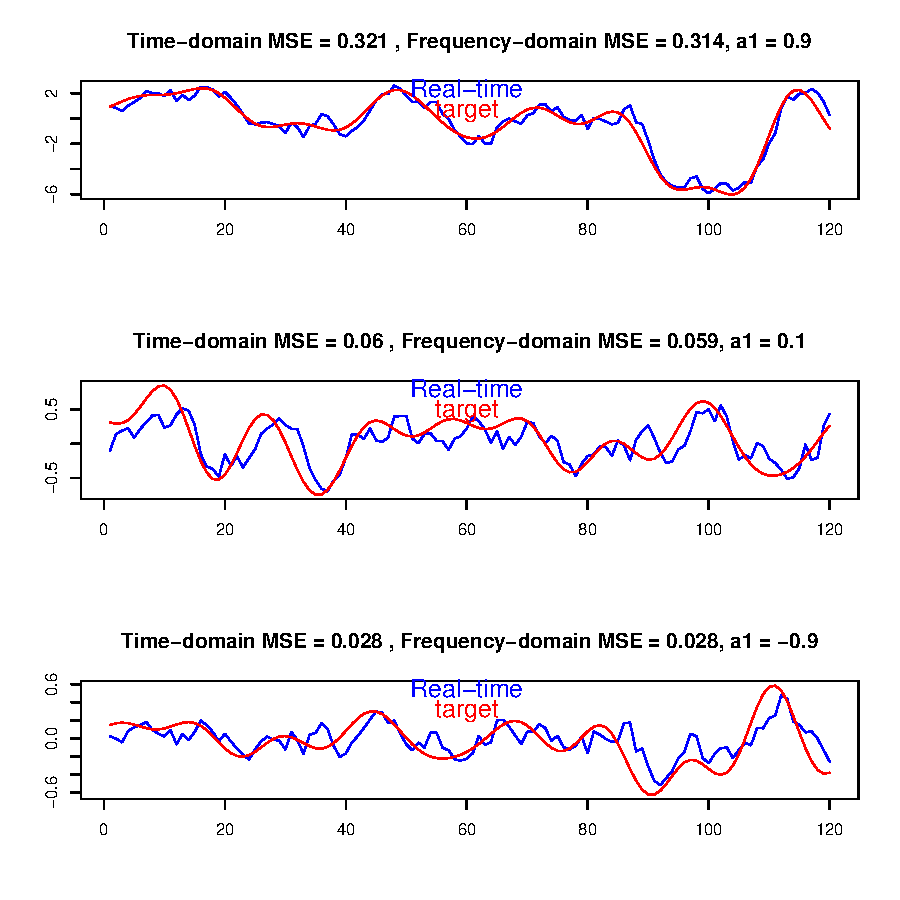
\includegraphics[height=6in, width=6in]{z_dfa_ar1_sym_output}\caption{Real-time filter output (blue) vs. targets (red) for a1=0.9 (top), a1=0.1 (middle) and a1=-0.9 (bottom)\label{z_dfa_ar1_sym_output}}\end{center}\end{figure}Visual inspection seems to conflict with MSE-performances: the real-time filter with the largest MSE (upper panel) appears to fit its target best. This conflict can be alleviated, to some extent, by adjusting for differences in scale of the time series\footnote{A relative (signal-to-noise) measure would seem more appropriate than the raw MSE, see later chapters.}. But it is obvious that the task of the filter in the upper panel seems easier, in some way, than that of the bottom filter, whose output is much noisier than its target. A more refined analysis reveals, also, that the real-time estimates appear to be systematically shifted to the right: they are delayed. Once again, the upper filter seems least affected. In summary: the difficulty of the estimation task seems to depend on the DGP as specified by the parameter $a_1$\footnote{Smaller $a_1$ correspond to noisier realizations $x_t$ which, in turn, lead to noisier real-time estimates $\hat{y}_t$ (increasingly difficult estimation problems).}. 
\item Compute and compare graphically amplitude and time-shift functions for all three realizations (processes), see fig.\ref{z_dfa_ar1_amp_shift}\footnote{Our plots are similar but not identical to the plots in \href{http://blog.zhaw.ch/sef/files/2014/10/DFA.pdf}{DFA}, section 4.1.1, exercise 1: here we use data in the middle of the long sample whereas in \href{http://blog.zhaw.ch/sef/files/2014/10/DFA.pdf}{DFA} the first 120 observations are used.}.
\begin{Schunk}
\begin{Sinput}
> omega_k<-pi*0:(len/2)/(len/2)
> file = paste("z_dfa_ar1_amp_shift.pdf", sep = "")
> pdf(file = paste(path.out,file,sep=""), paper = "special", width = 6, 
+     height = 6)
> par(mfrow=c(2,2))
> amp<-abs(trffkt)
> shift<-Arg(trffkt)/omega_k
> plot(amp[,1],type="l",main="Amplitude functions",
+ axes=F,xlab="Frequency",ylab="Amplitude",col="black",ylim=c(0,1))
> lines(amp[,2],col="orange")
> lines(amp[,3],col="green")
> lines(Gamma,col="violet")
> mtext("Amplitude a1=0.9", side = 3, line = -1,at=len/4,col="black")
> mtext("Amplitude a1=0.1", side = 3, line = -2,at=len/4,col="orange")
> mtext("Amplitude a1=-0.9", side = 3, line = -3,at=len/4,col="green")
> mtext("Target", side = 3, line = -4,at=len/4,col="violet")
> axis(1,at=c(0,1:6*len/12+1),labels=c("0","pi/6","2pi/6","3pi/6",
+ "4pi/6","5pi/6","pi"))
> axis(2)
> box()
> plot(shift[,1],type="l",main="Time-shifts",
+ axes=F,xlab="Frequency",ylab="Shift",col="black",
+ ylim=c(0,max(na.exclude(shift[,3]))))
> lines(shift[,2],col="orange")
> lines(shift[,3],col="green")
> lines(rep(0,len/2+1),col="violet")
> mtext("Shift a1=0.9", side = 3, line = -1,at=len/4,col="black")
> mtext("Shift a1=0.1", side = 3, line = -2,at=len/4,col="orange")
> mtext("Shift a1=-0.9", side = 3, line = -3,at=len/4,col="green")
> mtext("Target", side = 3, line = -4,at=len/4,col="violet")
> axis(1,at=c(0,1:6*len/12+1),labels=c("0","pi/6","2pi/6","3pi/6",
+ "4pi/6","5pi/6","pi"))
> axis(2)
> box()
> plot(periodogram[,1],type="l",main="Periodograms",
+ axes=F,xlab="Frequency",ylab="Periodogram",col="black",
+ ylim=c(0,max(periodogram[,3])/6))
> lines(periodogram[,2],col="orange")
> lines(periodogram[,3],col="green")
> mtext("Periodogram a1=0.9", side = 3, line = -1,at=len/4,col="black")
> mtext("Periodogram a1=0.1", side = 3, line = -2,at=len/4,col="orange")
> mtext("Periodogram a1=-0.9", side = 3, line = -3,at=len/4,col="green")
> axis(1,at=c(0,1:6*len/12+1),labels=c("0","pi/6","2pi/6","3pi/6",
+ "4pi/6","5pi/6","pi"))
> axis(2)
> box()
> invisible(dev.off())
\end{Sinput}
\end{Schunk}
\begin{figure}[H]\begin{center}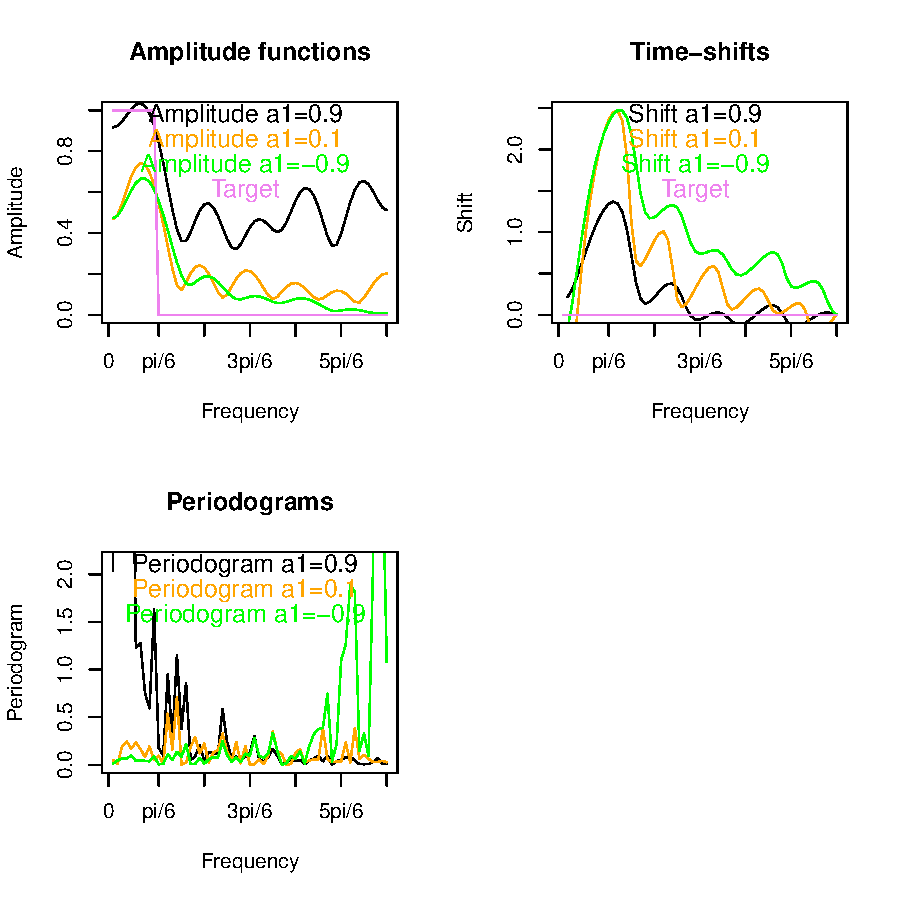
\includegraphics[height=6in, width=6in]{z_dfa_ar1_amp_shift.pdf}\caption{Amplitude (top left), time-shifts (top-right) and periodograms (bottom left) for
a1=0.9 (black), a1=0.1 (orange) and a1=-0.9 (green)\label{z_dfa_ar1_amp_shift}}\end{center}\end{figure}\begin{itemize}
\item Noise and delay of the real-time estimates $\hat{y}_t$ previously observed in fig.\ref{z_dfa_ar1_sym_output} are due to leaking amplitude functions (incomplete stop-band rejection) and to non-vanishing time-shift functions of the real-time filters, see fig.\ref{z_dfa_ar1_amp_shift}. Chapter \ref{ats_sec} proposes a more general optimization paradigm which will address these issues explicitly.
\item The time-shift (top right panel) of the black filter ($a_1=0.9$) remains comparatively small. Its amplitude function (top left panel) 
is the farthest away from the target in the stop-band $\omega>\pi/6$ but it is closest
to the target in the passband $\omega\leq\pi/6$: the optimization criterion seems to trade (poorer) high-frequency damping against (improved) passband properties. In summary: $\hat{\Gamma}(\cdot)$ tracks $\Gamma(\cdot)$ towards the loaded frequencies, as measured by the periodogram (bottom panel) in \ref{dfa_ms}. Similar findings apply to the other two processes.
\end{itemize}
\end{enumerate}



\section{MDFA: Problem-Structure and Target (MSE-Perspective)}\label{mdfa_ps_mse}




\subsection{Emphasizing the Filter Error}


The previous (univariate) DFA has been generalized to a multivariate framework in Wildi (2008.2), theorem 7.1, and in McElroy-Wildi (2015) (MDFA-paper).  We here briefly summarize the main results in the case of stationary processes (see chapters \ref{int_sec}, \ref{coint_sec} and \ref{ada_sec} for generalizations to non-stationary processes). \\

Let the target $y_t$ be defined by \ref{target} and let $x_t, w_{tj}$, $t=1,...,T$ and $j=1,...,m$ be an $m+1$-dimensional set of explanatory variables\footnote{The explicit link between $y_t$ and $x_t$, as defined by \ref{target}, justifies to distinguish $x_t$ from the other explanatory series.}. Consider
\begin{eqnarray}
\hat{\Gamma}_X(\omega_k)\Xi_{T
X}(\omega_k)+\sum_{n=1}^m
\hat{\Gamma}_{W_n}(\omega_k)\Xi_{TW_n}(\omega_k)\label{statcase}
\end{eqnarray}
where
\begin{eqnarray}
\hat{\Gamma}_X(\omega_k)&=&\sum_{j=0}^{L-1}b_{Xj} \exp(-ij\omega_k)\label{exp1}\\
\hat{\Gamma}_{W_n}(\omega_k)&=&\sum_{j=0}^{L-1}b_{w_nj} \exp(-ij\omega_k)\label{exp2}
\end{eqnarray}
are the (one-sided) transfer functions of the (real-time) filters, whose coefficients must be determined, and where $\Xi_{TX}(\omega_k)$, $\Xi_{TW_n}(\omega_k)$ are the corresponding DFTs of the data. The filter coefficients can be collected in a matrix $\mathbf{B}=(\mathbf{b}_{X},\mathbf{b}_{w_1},...,\mathbf{b}_{w_m})$ where $\mathbf{b}_{X}=(b_{X0},...,b_{X,L-1})'$ and $\mathbf{b}_{w_n}=(b_{w_n0},...,b_{w_n,L-1})'$ are the vectors of filter coefficients. Then the following multivariate MSE-criterion
\begin{equation}\label{dfanv}
\frac{2\pi}{T} \sum_{k=-T/2}^{T/2}
\left|\left(\Gamma(\omega_k)-\hat{\Gamma}_X(\omega_k)\right)\Xi_{T
X}(\omega_k)-\sum_{n=1}^m
\hat{\Gamma}_{W_n}(\omega_k)\Xi_{TW_n}(\omega_k)\right|^2 \to \min_{\mathbf{B}}
\end{equation}
generalizes the univariate DFA-MSE criterion \ref{dfa_ms}, see theorem 7.1 in Wildi (2008.2) and McElroy-Wildi (2015)\footnote{MDFA-paper.}.\\


\textbf{Remarks}:
\begin{itemize}
\item Due to the explicit link between $x_t$ and the target $y_t$, the former is generally informative about $y_t$. In some cases, however, we want to exclude $x_t$ from the set of explanatory variables (for example if $x_t$ is subject to large publication lags and/or large revisions, see chapter \ref{rev_sec}) and then we assume $\mathbf{b}_{X}=\mathbf{0}$ or, equivalently,  $\hat{\Gamma}_X\equiv 0$.
\item In the absence of additional explanatory series (i.e. $m=0$)  the multivariate criterion \ref{dfanv} reduces to \ref{dfa_ms}. The proposed (MSE-) MDFA-criterion thus generalizes the previous DFA. 
\end{itemize}






\subsection{One- and Multi-Step Ahead Forecast Criteria}\label{one_step}

The univariate and multivariate criteria \ref{dfa_ms} and \ref{dfanv} rely on a general target specification. The classic one-step ahead mean-square criterion could be replicated by specifying $\gamma_{-1}=1, \gamma_k=0, k\neq 0$ in \ref{target}:
\[y_t=\sum_{k=-\infty}^\infty\gamma_kx_{t-k}=x_{t+1}\]
In this case, criterion \ref{dfanv} becomes
\begin{equation}\label{dfanv_1s}
\frac{2\pi}{T} \sum_{k=-T/2}^{T/2}
\left|\left(\exp(i\omega_k)-\hat{\Gamma}_X(\omega_k)\right)\Xi_{T
X}(\omega_k)-\sum_{n=1}^m
\hat{\Gamma}_{W_n}(\omega_k)\Xi_{TW_n}(\omega_k)\right|^2 \to \min_{\mathbf{B}}
\end{equation}
where the anticipative \emph{allpass} target filter $\Gamma(\omega_k):=\exp(i\omega_k)$ rotates the DFT $\Xi_{T
X}(\omega_k)$ in the frequency-domain (shifts the data in the time-domain). A direct link to classical (pseudo-) maximum likelihood approaches is provided in chapter \ref{rep_sec} for details (replication of model-based performances by MDFA). To conclude, we note that  $h$-step ahead forecasting could be obtained by specifying the allpass target $\Gamma_h(\omega_k):=\exp(ih\omega_k)$. \\

\textbf{Remarks}
\begin{itemize}
\item Typically, in the time-domain, $h$ observations are lost when estimating the coefficients of a direct $h$-step ahead forecast equation. In contrast, the whole sample remains at disposal in the frequency-domain because time-shifts, of the data, are handled by rotations, of the (full-sample) DFTs.  
\item We here proposed forecasts of the \emph{original} data. In section \ref{for_now_smo} we generalize this concept to forecasts, nowcasts and backcasts of arbitrary signals.
\end{itemize}




\section{Matrix Notation and Generalized Least-Squares Solution}\label{matrix_not}

We here introduce a convenient matrix notation which will be useful when tackling filter constraints (see chapter \ref{con_sec}) as well as more sophisticated optimization criteria (customization, regularization, mixed-frequency). We then derive the solution of the MSE-criterion \ref{dfanv} in closed-form.

\subsection{Matrix Notation}\label{matrix_notation}

Because of the symmetry of its summands around $\omega_0=0$, criterion \ref{dfanv} can be rewritten in a numerically more efficient form
\begin{eqnarray}\label{dfanv_s}
&&\frac{2\pi}{T}\left|\left(\Gamma(0)-\hat{\Gamma}_X(0)\right)\Xi_{TX}(0)-\sum_{n=1}^m\hat{\Gamma}_{W_n}(0)\Xi_{TW_n}(0)\right|^2\nonumber\\
&+&2\frac{2\pi}{T} \sum_{k>0}^{T/2}\left|\left(\Gamma(\omega_k)-\hat{\Gamma}_X(\omega_k)\right)\Xi_{TX}(\omega_k)-\sum_{n=1}^m\hat{\Gamma}_{W_n}(\omega_k)\Xi_{TW_n}(\omega_k)\right|^2 \to \min_{\mathbf{B}}
\end{eqnarray}
Note that frequency zero is counted once, only,  whereas all strictly positive frequencies are duplicated\footnote{The unequal weighting of frequency zero explains the modified DFT in exercise \ref{ex_rep_dfa_1}, section \ref{ex_rep_dfa}.}. We now derive a more convenient vector notation for the above criterion.\\

Let $\mathbf{X}$ be a matrix whose $k$-th row $\mathbf{X}_k$ is defined as
\begin{eqnarray}\label{desmat}
\mathbf{X}_k&=&\sqrt{1+I_{k>0}}\cdot\nonumber\\
&&\textrm{Vec}_\textrm{row}\left(\begin{array}{ccccc} \Xi_{TX}(\omega_k)& \exp(-i\omega_k)\Xi_{TX}(\omega_k)&...& \exp(-i(L-1)\omega_k)\Xi_{TX}(\omega_k)\\
 \Xi_{TW_1}(\omega_k)& \exp(-i\omega_k)\Xi_{TW_1}(\omega_k)& ...& \exp(-i(L-1)\omega_k)\Xi_{TW_1}(\omega_k)\\
 \Xi_{TW_2}(\omega_k)& \exp(-i\omega_k)\Xi_{TW_2}(\omega_k)& ...& \exp(-i(L-1)\omega_k)\Xi_{TW_2}(\omega_k)\\
...&...&...&...\\
 \Xi_{TW_m}(\omega_k)& \exp(-i\omega_k)\Xi_{TW_m}(\omega_k&...& \exp(-i(L-1)\omega_k)\Xi_{TW_m}(\omega_k)\\
\end{array}\right)
\end{eqnarray}
where the $\textrm{Vec}_\textrm{row}$-operator appends rows (we use this notation in order to avoid margin-overflow) and where the `indicator' function $\sqrt{1+I_{k>0}}=\left\{\begin{array}{cc}1&k=0\\ \sqrt{2}&k=1,...,T/2\end{array}\right.$ accounts for the fact that frequency zero occurs once only in the criterion\footnote{Note that the square-root is required because we consider the DFT in \ref{desmat} i.e. the square root of the expressions in \ref{dfanv_s}.}. The length of the $k$-th row is $(m+1)L$ and the dimension of the design-matrix $\mathbf{X}$ is $(T/2+1)*(m+1)L$. Next, define a coefficient vector $\mathbf{b}$ and a target vector $\mathbf{Y}$
\begin{eqnarray*}
\mathbf{b}=\textrm{Vec}_\textrm{col}(\mathbf{B})&=&\textrm{Vec}_\textrm{col}\left(\begin{array}{ccccc} b_{X0}&b_{W_10}&b_{W_20}&...&b_{W_m0}\\
b_{X1}&b_{W_11}&b_{W_21}&...&b_{W_m1}\\
...&...&...&...&...\\
b_{XL-1}&b_{W_1L-1}&b_{W_2L-1}&...&b_{W_mL-1}
\end{array}\right)\\
\mathbf{Y}&=&\left(\begin{array}{c}\Gamma(\omega_0)\Xi_{TX}(\omega_0)\\ 
\sqrt{2}\Gamma(\omega_1)\Xi_{TX}(\omega_1)\\
\sqrt{2}\Gamma(\omega_2)\Xi_{TX}(\omega_2)\\
.\\
\sqrt{2}\Gamma(\omega_{T/2})\Xi_{TX}(\omega_{T/2})
\end{array}\right)
\end{eqnarray*}
where $\textrm{Vec}_\textrm{col}$ stacks the columns of the coefficient matrix $\mathbf{B}$. Note, once again, that all frequencies larger than zero are `duplicated' (scaled by $\sqrt{2}$) in $\mathbf{Y}$. Criterion \ref{dfanv} or, equivalently \ref{dfanv_s}, can now be expressed more conveniently in vector notation:
\begin{eqnarray}\label{irk}
(\mathbf{Y-Xb})'(\mathbf{Y-Xb})\to\min_{\mathbf{b}}
\end{eqnarray}
where $(\mathbf{Y-Xb})'$ is the Hermitian conjugate of $\mathbf{Y-Xb}$ (transpose and complex conjugate)\footnote{For simplicity we omitted the normalization $\frac{2\pi}{T}$ which is irrelevant for optimization.}. If all vectors and matrices were real (real numbers) then the solution to this minimization problem would be the well-known least-squares estimate
\begin{eqnarray*}
\mathbf{\hat{b}}=\left(\mathbf{X'X}\right)^{-1}\mathbf{X'}\mathbf{Y}
\end{eqnarray*}
Unfortunately, the above vectors and matrices are complex-valued. Before presenting a correct least-squares estimate we propose to rotate all DFT's \footnote{The criterion \ref{dfanv} is invariant to such a transformation.}: this transformation is not strictly necessary but it simplifies later expressions.
\begin{eqnarray}\label{dfanver}
&&\frac{2\pi}{T} \sum_{k=-T/2}^{T/2}
\left|\left(\Gamma(\omega_k)-\hat{\Gamma}_X(\omega_k)\right)\Xi_{T
X}(\omega_k)-\sum_{n=1}^m
\hat{\Gamma}_{W_n}(\omega_k)\Xi_{TW_n}(\omega_k)\right|^2\nonumber \\
&=&\frac{2\pi}{T} \sum_{k=-T/2}^{T/2}
\left|\left|\Gamma(\omega_k)\Xi_{TX}(\omega_k)\right| \exp\left(i*\arg\left(\Gamma(\omega_k)\Xi_{TX}(\omega_k)\right)\right)-\hat{\Gamma}_X(\omega_k)\Xi_{TX}(\omega_k)\right.\nonumber\\
&&\left.-\sum_{n=1}^m
\hat{\Gamma}_{W_n}(\omega_k)\Xi_{TW_n}(\omega_k)\right|^2 \nonumber\\
&=&\frac{2\pi}{T} \sum_{k=-T/2}^{T/2}
\left|\left|\Gamma(\omega_k)\Xi_{TX}(\omega_k)\right| -\hat{\Gamma}_X(\omega_k)\Xi_{TX}(\omega_k)\exp\left(-i*\arg\left(\Gamma(\omega_k)\Xi_{T
X}(\omega_k)\right)\right)\right.\nonumber\\
&&\left.-\sum_{n=1}^m
\hat{\Gamma}_{W_n}(\omega_k)\Xi_{TW_n}(\omega_k)\exp\left(-i*\arg\left(\Gamma(\omega_k)\Xi_{T
X}(\omega_k)\right)\right)\right|^2 \label{i-mdfa}
\end{eqnarray}
where the arg-function corresponds to the phase (angle) of a complex number and where the function is applied component-by-component to the complex-valued vector.  
Let us define a rotated design-matrix $\mathbf{X}_{\textrm{rot}}$ and a rotated target vector $\mathbf{Y}_{\textrm{rot}}$
\begin{eqnarray}\label{desmatrot}
\mathbf{X}_{k,\textrm{rot}}&=&\mathbf{X}_k \exp\left(-i*\arg\left(\Gamma(\omega_k)\Xi_{TX}(\omega_k)\right)\right)
\end{eqnarray}
where $\mathbf{X}_{k,\textrm{rot}}$ designates the $k$-th row of $\mathbf{X}_{\textrm{rot}}$ and where
\begin{eqnarray}\label{desmatrot_y}
 \mathbf{Y}_{\textrm{rot}}=\left|\mathbf{Y}\right|
\end{eqnarray}
is a (real) positive target vector. 



\subsection{Generalized Least Squares Solution}\label{gen_le_sq_sol}

The optimization criterion becomes
\begin{eqnarray}\label{regms}
(\mathbf{Y_{\textrm{rot}}-X_{\textrm{rot}}b})'(\mathbf{Y_{\textrm{rot}}-X_{\textrm{rot}}b})\to\min_{\mathbf{b}}
\end{eqnarray}
The general (matrix derivative) formula for tackling this complex-valued minimization problem is\footnote{A convenient survey of matrix derivatives is to be found on the wikipedia-site \href{http://en.wikipedia.org/wiki/Matrix_calculus}{Matrix calculus}.}
\begin{eqnarray}\label{least_squares_b}
d/d\mathbf{b}~\textrm{Criterion}&=&d/d\mathbf{b}~ (\mathbf{Y_{\textrm{rot}}-X_{\textrm{rot}}b})'(\mathbf{Y_{\textrm{rot}}-X_{\textrm{rot}}b})\\
&=&-\mathbf{(Y_{\textrm{rot}}-X_{\textrm{rot}}b)'X_{\textrm{rot}}}-\mathbf{(Y_{\textrm{rot}}-X_{\textrm{rot}}b)^T\overline{X_{\textrm{rot}}}}\nonumber\\
&=&-2\mathbf{Y_{\textrm{rot}}'\Re\left(X_{\textrm{rot}}\right)}+2\mathbf{b'\Re(X_{\textrm{rot}}'X_{\textrm{rot}})}\nonumber
\end{eqnarray}
where  $\mathbf{X_{\textrm{rot}}}'$ is the Hermitian conjugate, $\mathbf{X_{\textrm{rot}}^T}$ is the transposed and $\overline{\mathbf{X_{\textrm{rot}}}}$ is the complex conjugate matrix;   $\Re\left(\cdot\right)$ means the real part of a complex number. The generalized least-squares estimate is obtained by equating the previous expression to zero
\begin{eqnarray}\label{bregms}
\mathbf{\hat{b}}&=&\mathbf{\left(\Re(X_{\textrm{rot}}'X_{\textrm{rot}})\right)^{-1}\Re(X_{\textrm{rot}})'Y_{\textrm{rot}}}
\end{eqnarray}
The least-squares estimate $\mathbf{\hat{b}}$ is the solution of the MDFA-MSE signal extraction problem \ref{dfanv} (or \ref{dfa_ms} in the univariate case).


\subsection{R-Code}

\subsubsection{DFA}

The proposed matrix notation and the MSE (generalized least-squares) estimate $\hat{\mathbf{b}}$ can be traced-back in the R-code of the (MSE-) DFA proposed in section \ref{dfa_intro}:

\begin{Schunk}
\begin{Sinput}
> dfa_ms
\end{Sinput}
\begin{Soutput}
function (L, periodogram, Lag, Gamma) 
{
    K <- length(periodogram) - 1
    X <- exp(-(0+1i) * Lag * pi * (0:(K))/(K)) * rep(1, K + 1) * 
        sqrt(periodogram)
    X_y <- exp(-(0+1i) * Lag * pi * (0:(K))/(K)) * rep(1, K + 
        1)
    for (l in 2:L) {
        X <- cbind(X, (cos((l - 1 - Lag) * pi * (0:(K))/(K)) + 
            (0+1i) * sin((l - 1 - Lag) * pi * (0:(K))/(K))) * 
            sqrt(periodogram))
        X_y <- cbind(X_y, (cos((l - 1 - Lag) * pi * (0:(K))/(K)) + 
            (0+1i) * sin((l - 1 - Lag) * pi * (0:(K))/(K))))
    }
    xtx <- t(Re(X)) %*% Re(X) + t(Im(X)) %*% Im(X)
    b <- as.vector(solve(xtx) %*% (t(Re(X_y)) %*% (Gamma * periodogram)))
    trffkt <- 1:(K + 1)
    trffkt[1] <- sum(b)
    for (k in 1:(K)) {
        trffkt[k + 1] <- (b %*% exp((0+1i) * k * (0:(length(b) - 
            1)) * pi/(K)))
    }
    return(list(b = b, trffkt = trffkt))
}
<environment: namespace:MDFA>
\end{Soutput}
\end{Schunk}
The code replicates the above formulas up to the particular weighting of frequency zero (see exercise \ref{ex_rep_dfa_1}, section \ref{ex_rep_dfa_11}).

\subsubsection{MDFA}

The least-squares solution \ref{bregms} is nested as a special case in the generic MDFA estimation routine introduced in section \ref{mdfa_intro}. The DFA is nested too, see section  \ref{ex_rep_dfa} (replication). Other nested solutions replicate classic model-based approaches, see chapter \ref{rep_sec}. Conceptually, `nesting' is obtained by specifying hyperparameters in the head of the function call.


\section{Grand-Mean Parametrization}\label{gm_par}


This particular feature has been discontinued and has been substituted by the more powerful Regularization Troika, see chapter \ref{reg_sec}. Nevertheless, one may find vestiges in our R-package (and the functionality could still be activated). Therefore we briefly review the main concepts.\\

The term `Grand-Mean' refers to a reparametrization or recoding of the filter coefficients whereby the original coefficients are expressed as deviations about a central (grand-mean) value. Specifically, let $b_l^u$, $l=0,...,L-1$, $u=0,...,m$ denote the lag-$l$ coefficient assigned to series $u$, whereby $u=0$ corresponds to $x_t$ and $u=1,...,m$ stands for $w_{tu}$. The coefficients could be rewritten in the form
\begin{eqnarray}\label{repara}
b_{l}^u&=&\left\{\begin{array} {cc}b_l+\delta b_l^u, &u>0\\
b_l-\sum_{u=1}^m\delta b_l^{u}, &u=0\end{array}\right.
\end{eqnarray}
where $b_l$, $l=0,...,L-1$ is a central (grand-mean) vector of coefficients and where $\delta b_l^u$ are the deviations about the central coefficient-vector. For obvious reasons we here assume $m>0$ (truly multivariate design). Note that \ref{repara} imposes  $\delta b_l^0=-\sum_{u=1}^m\delta b_l^{u}$ which means that $b_l$ is in the `center' of the coefficients. Similarly,  $\delta b_l^u$, $u>0$ can be interpreted as series-specific `effects'. We can express the above re-parametrization in terms of
\begin{eqnarray}
\mathbf{b}&=&\mathbf{A} \mathbf{\tilde{b}}\label{btild}\\
\mathbf{A}&=&\left(\begin{array}{cccccc} \mathbf{Id}&\mathbf{-Id}&\mathbf{-Id}&...             &...&\mathbf{-Id}\\
                                                            \mathbf{Id}&\mathbf{Id}&\mathbf{0}&\mathbf{0}&...&\mathbf{0}\\
                                                            \mathbf{Id}&\mathbf{0}&\mathbf{Id}&\mathbf{0}&...&\mathbf{0}\\
:::\\
                                                            \mathbf{Id}&\mathbf{0}&\mathbf{0}&...&...&\mathbf{Id}\\
\end{array}\right)\nonumber\\
\mathbf{b}'&=&\left(b_0^0, b_1^0 ,...,b_{L-1}^0~|~ b_0^1, b_1^1,...,b_{L-1}^1~|~...~|~...~|~...~|~  b_0^m, b_1^m,..., b_{L-1}^m\right)'\nonumber\\
\mathbf{\tilde{b}}'&=&\left(b_0, b_1 ,...,b_{L-1}~|~ \delta b_0^1,\delta b_1^1,...,\delta b_{L-1}^1~|~ \delta b_0^2,\delta b_1^2,...,\delta b_{L-1}^2~|~...~|~...~|~...~|~ \delta b_0^m,\delta b_1^m,...,\delta b_{L-1}^m\right)'\nonumber
\end{eqnarray} 
where $\mathbf{Id}$ is an $L*L$ identity. In principle, a separation of the series-specific effects from the grand-mean would point towards an explicit control of the cross-sectional adaptivity of the multivariate filter (for example by imposing a zero-shrinkage of $\delta b_l^u$). In this context we may refer to chapter \ref{reg_sec} for a more general approach and therefore we defer a more comprehensive discussion and treatment of the topic.



\section{Replication of DFA by MDFA}\label{ex_rep_dfa}



We rely on the data in the previous exercises, see section \ref{ex_dfa}, and \emph{replicate} the obtained DFA-results (criterion \ref{dfa_ms}) by MDFA (criterion \ref{dfanv}). 

\subsection{Exercises}\label{ex_rep_dfa_11}

\begin{enumerate}
\item \label{ex_rep_dfa_1}Define the data-matrix (target and explanatory variable) and compute the DFTs. For ease of exposition we consider the first AR(1)-process only ($a_1=0.9$).
\begin{Schunk}
\begin{Sinput}
> # Select the first process
> i_process<-1
> # Define the data-matrix:
> # The first column must be the target series. 
> # Columns 2,3,... are the explanatory series. In a univariate setting
> # target and explanatory variable are identical
> data_matrix<-cbind(x[,i_process],x[,i_process])
> # Determine the in-sample period (fully in sample)
> insample<-nrow(data_matrix)
> # Compute the DFT by relying on the multivariate DFT-function: 
> #   d=0 for stationary data (default settings)
> weight_func<-spec_comp(insample, data_matrix, d)$weight_func 
\end{Sinput}
\end{Schunk}
\item Estimate optimal filter coefficients and compare DFA- and MDFA-estimates. 
\begin{Schunk}
\begin{Sinput}
> # Source the default (MSE-) parameter settings
> source(file=paste(path.pgm,"control_default.r",sep=""))
> # Estimate filter coefficients:
> mdfa_obj<-MDFA_mse(L,weight_func,Lag,Gamma)$mdfa_obj 
> # Filter coefficients: compare MDFA and previous DFA
> b_mat<-cbind(mdfa_obj$b,b[,i_process])
> dimnames(b_mat)[[2]]<-c("MDFA","DFA")
> dimnames(b_mat)[[1]]<-paste("lag ",0:(L-1),sep="")
> as.matrix(round(b_mat,5))
\end{Sinput}
\begin{Soutput}
           MDFA      DFA
lag 0   0.53821  0.53821
lag 1   0.10039  0.10039
lag 2   0.17419  0.17419
lag 3   0.11221  0.11221
lag 4   0.08075  0.08075
lag 5   0.01972  0.01972
lag 6   0.05718  0.05718
lag 7  -0.03330 -0.03330
lag 8  -0.04889 -0.04889
lag 9  -0.03821 -0.03821
lag 10 -0.08752 -0.08752
lag 11  0.04178  0.04178
\end{Soutput}
\end{Schunk}
The MDFA replicates DFA, as desired. Note that we could refer to the context-specific $MDFA\textunderscore mse$ function
\begin{Schunk}
\begin{Sinput}
> mdfa_obj_mse<-MDFA_mse(L,weight_func,Lag,Gamma)$mdfa_obj 
\end{Sinput}
\end{Schunk}
which abbreviates the lengthy list of arguments of the generic $mdfa\textunderscore analytic$-call to those required in a MSE-framework. As can be seen, estimated coefficients are identical:
\begin{Schunk}
\begin{Sinput}
> b_mat<-cbind(b_mat,mdfa_obj_mse$b)
> dimnames(b_mat)[[2]][3]<-"MDFA_mse"
> dimnames(b_mat)[[1]]<-paste("lag ",0:(L-1),sep="")
> head(as.matrix(round(b_mat,5)))
\end{Sinput}
\begin{Soutput}
         MDFA     DFA MDFA_mse
lag 0 0.53821 0.53821  0.53821
lag 1 0.10039 0.10039  0.10039
lag 2 0.17419 0.17419  0.17419
lag 3 0.11221 0.11221  0.11221
lag 4 0.08075 0.08075  0.08075
lag 5 0.01972 0.01972  0.01972
\end{Soutput}
\end{Schunk}
\item The value of the multivariate criterion \ref{dfanv} is computed explicitly by the MDFA-function:
\begin{Schunk}
\begin{Sinput}
> # Criterion value
> criterion_mdfa<-mdfa_obj$MS_error  
> # DFA-numbers are stored in perf_mat
> crit_mdfa<-matrix(c(criterion_mdfa,perf_mat[i_process,1],
+                     perf_mat[i_process,2]),ncol=1)
> dimnames(crit_mdfa)[[1]]<-c("MDFA criterion",
+                             "DFA criterion","sample MSE")
> dimnames(crit_mdfa)[[2]]<-"MSE estimates"
> t(round(crit_mdfa,3))
\end{Sinput}
\begin{Soutput}
              MDFA criterion DFA criterion sample MSE
MSE estimates          0.314         0.314      0.321
\end{Soutput}
\end{Schunk}
\end{enumerate}




\section{Qualitative Easing by Leading Indicators: an Empirical Study}\label{leading_ind}

We attempt to quantify performance gains obtained by inclusion of a leading indicator into the univariate design of the previous section. Specifically, we construct a new explanatory  series $w_{1t}$ 
\begin{equation}\label{def_led_i}
w_{1t}=x_{t+\delta}+s\cdot\epsilon_{t+\delta}
\end{equation}
where $x_t$ is the data of the previous univariate design, $\epsilon_t$ is an idiosyncratic noise component (iid zero-mean Gaussian standardized), $s$ is a scaling\footnote{A larger $s$ implies that the indicator is less informative about the target $y_t$.}) and $\delta$ is a time-shift. 
In the first exercise, section \ref{bimdfaudfa}, we select $s=0.1$ (a weak idiosyncratic component) and $\delta=1$ (lead by one time unit). Alternative settings are analyzed in section \ref{lead_snr}.

\subsection{Bivariate MDFA vs. Univariate DFA}\label{bimdfaudfa}

\begin{enumerate}
\item Use the data in the previous section \ref{ex_rep_dfa}, construct the leading indicator \ref{def_led_i} and specify the (3-dim) data-matrix.
\begin{Schunk}
\begin{Sinput}
> set.seed(12)
> # Select the AR(1)-process with coefficient 0.9
> i_process<-1
> # Scaling of the idiosyncratic noise
> scale_idiosyncratic<-0.1
> eps<-rnorm(nrow(xh))
> indicator<-xh[,i_process]+scale_idiosyncratic*eps
> # Data: first column=target, second column=x, 
> #   third column=shifted (leading) indicator
> data_matrix<-cbind(xh[,i_process],xh[,i_process],c(indicator[2:nrow(xh)],NA))
> dimnames(data_matrix)[[2]]<-c("target","x","leading indicator")
> # Extract 120 observations from the long sample
> data_matrix_120<-data_matrix[lenh/2+(-len/2):((len/2)-1),]
> head(round(data_matrix_120,4))
\end{Sinput}
\begin{Soutput}
     target      x leading indicator
[1,] 1.0687 1.0687            0.8137
[2,] 0.9497 0.9497            0.6150
[3,] 0.6628 0.6628            1.7381
[4,] 1.6465 1.6465            1.6748
[5,] 1.7680 1.7680            1.7033
[6,] 1.8317 1.8317            2.4977
\end{Soutput}
\end{Schunk}
The first two series are identical; the new third one leads by one-time unit and it is contaminated by noise.
\item Compute the DFTs of the data.
\begin{Schunk}
\begin{Sinput}
> # Fully in sample
> insample<-nrow(data_matrix_120)
> # d=0 for stationary series: see default settings
> weight_func<-spec_comp(insample, data_matrix_120, d)$weight_func 
\end{Sinput}
\end{Schunk}
\item Estimate optimal (MSE-) filter coefficients.
\begin{Schunk}
\begin{Sinput}
> # Source the default (MSE-) parameter settings
> source(file=paste(path.pgm,"control_default.r",sep=""))
> # Estimate filter coefficients
> mdfa_obj<-MDFA_mse(L,weight_func,Lag,Gamma)$mdfa_obj 
> # Filter coefficients
> b_mat<-mdfa_obj$b
> dimnames(b_mat)[[2]]<-c("x","leading indicator")
> dimnames(b_mat)[[1]]<-paste("Lag ",0:(L-1),sep="")#dim(b_mat)
> head(b_mat)
\end{Sinput}
\begin{Soutput}
               x leading indicator
Lag 0 0.20556332        0.39969599
Lag 1 0.35970890       -0.08021796
Lag 2 0.21659593       -0.18695421
Lag 3 0.14359475       -0.06108555
Lag 4 0.13724690       -0.02475913
Lag 5 0.06399915       -0.09717151
\end{Soutput}
\end{Schunk}
The top-coefficient (the first six only are shown) in the second column assigns most weight to the last observation of the leading-indicator: this observation is particular because it leads the original data. In direct comparison with the first column, the other coefficients are generally smaller (in absolute value) because the leading-indicator is contaminated by noise (the coefficients in the first column must be shifted down in order to make meaningful cross-sectional comparisons).  
\item Compute the minimal criterion value.
\begin{Schunk}
\begin{Sinput}
> # Criterion value
> round(mdfa_obj$MS_error,3)
\end{Sinput}
\begin{Soutput}
[1] 0.145
\end{Soutput}
\end{Schunk}
The new criterion value is substantially smaller than the DFA (0.314, see previous exercise): efficiency gains exceed $50\%$ (reduction of mean-square filter error).
\item  Verify that the mean-square sample error is indeed smaller (recall that the sample MSE is generally not observable because it involves knowledge of the target $y_t$).
\begin{itemize}
\item Apply the (bivariate) filter to the data
\begin{Schunk}
\begin{Sinput}
> yhat_multivariate_leading_indicator<-rep(NA,len)
> for (j in 1:len)
+   yhat_multivariate_leading_indicator[j]<-sum(apply(b_mat*
+                   data_matrix[lenh/2+(-len/2)-1+j:(j-L+1),2:3],1,sum))
\end{Sinput}
\end{Schunk}
\item Derive the (time-domain) sample mean-square error and compare performances with the DFA, above.
\begin{Schunk}
\begin{Sinput}
> y_target_leading_indicator<-y[,i_process]
> perf_mse<-matrix(c(mean(na.exclude((yhat_multivariate_leading_indicator-
+           y_target_leading_indicator))^2),
+           mean(na.exclude((yhat[,i_process]-
+           y_target_leading_indicator))^2)),nrow=1)
> dimnames(perf_mse)[[2]]<-c("bivariate MDFA","DFA")
> dimnames(perf_mse)[[1]]<-"Sample MSE"
> round(perf_mse,3)
\end{Sinput}
\begin{Soutput}
           bivariate MDFA   DFA
Sample MSE          0.139 0.321
\end{Soutput}
\end{Schunk}
Sample MSE-performances of the bivariate design are substantially improved, as expected: the leading indicator is informative (this result depends on the magnitude of the idiosyncratic noise in the construction of the indicator, of course). Also, the criterion value 0.145 is fairly close to the sample MSE 0.139, as desired.    
\end{itemize}
\item Plot and compare target $y_t$ as well as DFA and MDFA real-time estimates $\hat{y}_t$.
\begin{Schunk}
\begin{Sinput}
> file = paste("z_mdfadfa_ar1_sym_output.pdf", sep = "")
> pdf(file = paste(path.out,file,sep=""), paper = "special", width = 6, height = 6)
> i<-1
> ymin<-min(min(y[,i]),min(na.exclude(yhat)[,i]))
> ymax<-max(max(y[,i]),max(na.exclude(yhat)[,i]))
> ts.plot(yhat[,i],main=paste("Sample MSE MDFA: ",ylab="",
+ round(perf_mse[1],3),", DFA: ",round(perf_mse[2],3),sep=""),col="blue",
+       ylim=c(ymin,ymax))
> lines(y[,i],col="red")
> lines(yhat_multivariate_leading_indicator,col="green")
> mtext("DFA", side = 3, line = -2,at=len/2,col="blue")
> mtext("target", side = 3, line = -1,at=len/2,col="red")
> mtext("MDFA", side = 3, line = -3,at=len/2,col="green")
> invisible(dev.off())
\end{Sinput}
\end{Schunk}


\begin{figure}[H]\begin{center}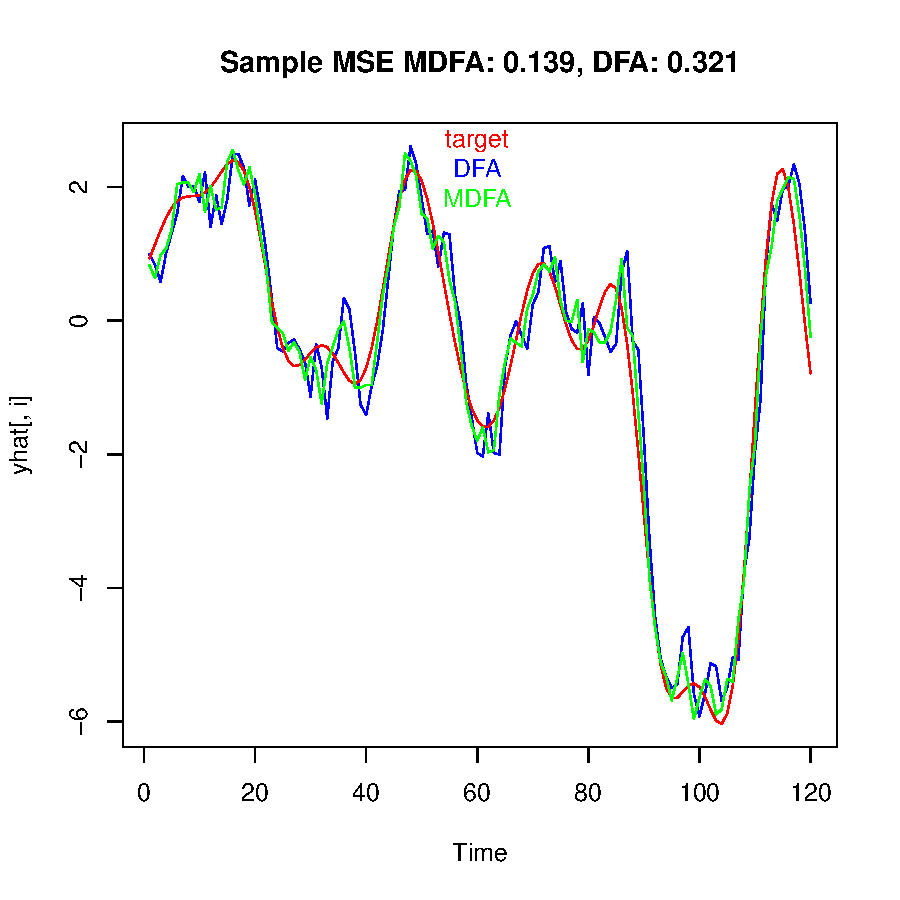
\includegraphics[height=3in, width=6in]{z_mdfadfa_ar1_sym_output}\caption{Target (red) vs. DFA (blue) and bivariate MDFA (green) for the first process (a1=0.9)\label{z_mdfadfa_ar1_sym_output}}\end{center}\end{figure}The MDFA-output (green) is both smoother and faster than the DFA (blue): noisy ripples are smaller in magnitude and turning points can be detected earlier (lead).

\item Verify that filter coefficients of the bivariate design are optimal: this is left as an exercise to the reader (any other set of bivariate filter coefficients, of length 12, should increase the criterion value 0.145 and/or the sample MSE 0.139).

\end{enumerate}




\subsection{Measuring Lead and Signal-to-Noise Effects of a Leading Indicator}\label{lead_snr}

Empirical evidence or experience suggest that `lead' and `signal-to-noise ratio' are conflicting requirements: faster indicators are generally noisier. We here attempt to disentangle and to quantify both effects, in terms of MSE-performances, by relying on our previous toy-model
\[w_{1t}=x_{t+\delta}+s\cdot\epsilon_{t+\delta}\]
For fixed $x_t$ we can alter the shift $\delta$ and the (inverse) signal-to-noise ratio $s$. To be more specific, we want to analyze non-integer shifts $\delta_j=j/4,j=0,1,2,3,4$\footnote{Arbitrary $\delta$ can be implemented very easily in the frequency-domain because shifts become rotations of the data.} in order to be able to quantify \emph{weekly} up-dating effects of a \emph{monthly} indicator in the framework of a mixed-frequency approach, see chapter \ref{mix_sec}\footnote{A fractional lead of $\delta=1/4$ corresponds to an anticipation by one week in an otherwise monthly framework: this lead by one week could be obtained by exploiting weekly up-dates of a `high-frequency' weekly indicator correlating with the interesting monthly target series.}. In the context of the following exercise we are interested in quantifying gains obtained by up-dating information on a weekly basis as a function of the signal-to-noise ratio of the high-frequency (weekly) indicator.


\begin{enumerate}
\item Specify candidate time-shifts $\delta_j=j/4,j=0,...,4$ and (inverse) signal-to-noise ratios $\mathbf{s}=(0,0.1,0.5,1,2)/\sqrt{Var(x_t)}$
\begin{Schunk}
\begin{Sinput}
> # Inverse SNR: the variance of the standardized noise is one: 
> #   we thus normalize by the standard deviation of the data x 
> #   (second column of the data matrix) 
> scale_idiosyncratic_vec<-c(0,0.1,0.5,1,2)/sqrt(var(data_matrix_120[,2]))
> # We select fractional leads: multiples of 0.25 
> #   A fractional lead of 0.25 corresponds roughly to a week 
> #   on a monthly time scale
> delta_vec<-0.25*0:4
\end{Sinput}
\end{Schunk}
\item Generate leading indicators for all combinations of $(\delta_j,s_i)$ and compute corresponding mean-square filter errors (criterion values).
\begin{Schunk}
\begin{Sinput}
> # Initialize the performance matrix
> lead_snr_mat<-matrix(ncol=length(scale_idiosyncratic_vec),
+                      nrow=length(delta_vec))
> dimnames(lead_snr_mat)[[2]]<-paste("1/SNR=",
+             sqrt(var(data_matrix_120[,1]))*scale_idiosyncratic_vec,paste="")
> dimnames(lead_snr_mat)[[2]][1]<-paste("Univ. design: ",
+             dimnames(lead_snr_mat)[[2]][1],sep="")
> dimnames(lead_snr_mat)[[1]]<-paste("Lead ",delta_vec,paste="")
> # Generate the idiosyncratic noise
> set.seed(20)
> eps<-rnorm(nrow(data_matrix_120))
> # Loop over all combinations of leads and SNR-ratios
> for (i in 1:length(scale_idiosyncratic_vec))#i<-1
+ {
+   for (j in 1:length(delta_vec))#j<-1
+   {
+ # Add the (suitably scaled) noise: no lead yet.    
+     indicator<-data_matrix_120[,2]+scale_idiosyncratic_vec[i]*eps
+ # Overwrite the indicator column with the new time series
+     data_matrix_120[,3]<-indicator
+ # Compute the DFTs (full in-sample, for stationary series d=0)
+     insample<-nrow(data_matrix_120)
+     weight_func<-spec_comp(insample, data_matrix_120, d)$weight_func
+ # Compute the discrete frequency-grid omega_k: from zero to pi
+     omega_k<-(0:(nrow(weight_func)-1))*pi/(nrow(weight_func)-1)
+ # Introduce the fractional time-shift by rotation of the DFT 
+ #   of the indicator (last column)
+     weight_func[,ncol(weight_func)]<-exp(-1.i*delta_vec[j]*omega_k)*
+                   weight_func[,ncol(weight_func)]
+ # If the idiosyncratic noise is zero, then we use a univariate design
+   if (i==1)
+      weight_func<-weight_func[,-2]
+ # Compute optimal filters and derive the (frequency-domain) MSE
+     mdfa_obj<-MDFA_mse(L,weight_func,Lag,Gamma)$mdfa_obj 
+ # Store the MSE
+     lead_snr_mat[j,i]<-mdfa_obj$MS_error
+   }
+ }
\end{Sinput}
\end{Schunk}
\item Collect all MSEs (criterion values) in table \ref{lead_snr_mat} and analyse the obtained results.
% latex table generated in R 3.3.2 by xtable 1.8-2 package
% Fri Dec 16 15:20:55 2016
\begin{table}[ht]
\centering
\begin{tabular}{rrrrrr}
  \hline
 & Univ. design: 1/SNR= 0  & 1/SNR= 0.1  & 1/SNR= 0.5  & 1/SNR= 1  & 1/SNR= 2  \\ 
  \hline
Lead  0  & 0.314 & 0.263 & 0.263 & 0.263 & 0.263 \\ 
  Lead  0.25  & 0.261 & 0.173 & 0.229 & 0.254 & 0.264 \\ 
  Lead  0.5  & 0.215 & 0.139 & 0.188 & 0.215 & 0.248 \\ 
  Lead  0.75  & 0.177 & 0.124 & 0.157 & 0.179 & 0.220 \\ 
  Lead  1  & 0.146 & 0.121 & 0.129 & 0.146 & 0.189 \\ 
   \hline
\end{tabular}
\caption{Effect of lead and of (inverse) signal-to-noise ratio on filter MSE} 
\label{lead_snr_mat}
\end{table}\\
\textbf{Analysis: Design}
\begin{itemize}
\item If the noise and the lead vanish ($s=\delta=0$), then the design is singular because 
\[w_{1t}=x_t+s\epsilon_t=x_t
\]
Therefore we have to skip one of the redundant explanatory variables in the DFT.
\item If the idiosyncratic noise component vanishes but the lead does not ($s=0, \delta>0$) then, in principle, the data is not perfectly colinear, at least in the time-domain. In the frequency-domain, though, the two DFT-columns are linearly dependent (rotation) and therefore the proposed design is still singular\footnote{The DFT assumes that the data is periodic: therefore original and shifted data are perfectly colinear. The singularity could be avoided by computing DFTs of original and shifted series explicitly (instead of rotating the DFT).}. Therefore, all results in the first column correspond to \emph{univariate} designs, where the single explanatory variable is the \emph{noise-free} leading indicator.
\item Performances reported in columns 2-5 of the first row (0.263: $\delta=0$) are identical because all designs are strictly equivalent in informational terms: one can subtract $x_t$ (second data-column) from $w_{1t}=x_t+s\epsilon_t$ to obtain $s\epsilon_t$ i.e. the data-matrix $(x_t,w_{1t})$ could be substituted by $(x_t,\epsilon_t)$ for all $s\neq 0$. 
\item Since $\epsilon_t$ is independent of $x_t$ (different random seed) one expects that performances of bivariate designs (columns 2-5) and of the univariate design (column 1) in the first row ($\delta=0$) should be identical, at least in theory. In practice, the spurious decrease 0.263$-$0.314$=$-0.05 of the bivariate designs is entirely due to \emph{overfitting}, see chapter \ref{reg_sec} for a comprehensive development of the topic. 
\end{itemize}
\textbf{Analysis: Results}
\begin{itemize}
\item Column 1 in the above table corresponds to a \emph{univariate} design; columns 2-5 are \emph{bivariate} designs. The first column measures time-shift effects of a single \emph{noise-free} leading indicator\footnote{The DFA cannot be used to replicate these results if the explanatory variable is shifted because target and explanatory variables wouldn't be identical.}. Columns 2-4 consider a classic bivariate design, where the original data is augmented by a noisy leading indicator.
\item The top-left number (0.314) (univariate design without lead) replicates performances as reported in section \ref{ex_rep_dfa}. 
\item The MSE generally decreases with increasing lead (increasing $\delta$) and/or with decreasing (inverse) signal-to-noise ratio (smaller $s$, except the degenerate case $s=0$: overfitting). A stronger noise could be compensated, to some extent, by a larger lead, at least in a mean-square perspective. As an example, an increase of the (inverse) SNR from 0.1 to 1 could be compensated by a relative lead by half a month, see cells (3,2) and (5,4) in the above table.
\item Leads larger than one time unit (one month) do not seem to add significant value if the noise is weak (second column). If the noise is strong (last column) larger leads may be required in order to compensate for the augmented noise\footnote{Stronger noise suppression by the filter induces larger delays of the output signal which must be compensated by an increasing lead of the series.}. 
\item Ignoring weekly up-dates of the filter-output $\hat{y}_t$, within the running month, could be costly in terms of performance-losses: if the noise component is weak (second column) then a lead of 0.25 instead of 0 (up-date at the week following the monthly release) would reduce MSE from 0.263 to 0.173 under the above experimental setting. If noise and signal are equally strong (4-th column) then an up-date of $\hat{y}_t$ in the middle of the month (lead 0.5 instead of 0) would reduce the MSE from 0.263 to 0.215.    
\end{itemize}
These results suggests pertinence of a mixed-frequency approach for which the filter output is aligned on an in-flowing high-frequency data-stream and continuously up-dated in real-time, see chapter \ref{mix_sec}. 
\end{enumerate}

\section{Summary}

\begin{itemize}
\item We emphasized MSE-performances of unconstrained, unregularized and stationary designs.
\item We provided a DFA-reminder and confirmed empirical pertinence of the abstract uniform superconsistency argument. We illustrated and interpreted the univariate DFA-criterion.
\item We generalized the DFA-criterion to a multivariate framework and derived a closed-form solution. 
\item We replicated the DFA by the more general MDFA and we quantified efficiency gains obtained by a bivariate leading-indicator design (over the univariate approach).
\item Our results suggested pertinence and practical relevance of a mixed-frequency approach, for which filter-outputs would be up-dated along a high-frequency data-stream.
\end{itemize}
For ease of exposition, all  examples emphasized in-sample and single realization experiments. Empirical distributions of in-sample as well as of out-of-sample performances are to be found in chapters \ref{ats_sec} and following.

%----------------------------------------



\chapter{Optimal Time-Dependent Filter Sequences}\label{vintages_triangle_revision}\label{fil_sec}




\section{Introduction}

Until yet we analyzed real-time \emph{fixed} filters
\[\hat{y}_t=\sum_{k=0}^{L-1}b_kx_{t-k}~,~t=L,...,T\]
whose coefficients $b_k$ did not dependent on time $t$. In practice, however, it is not uncommon  to rely on \emph{sequences} of time-dependent filters, whereby each filter in the sequence is optimized for a particular time point $t$ in the sample. In such a case, adding a new observation $x_{T+1}$ generally affects all (or part of the) previous estimates $\hat{y}_t$, for $t=L,...,T$, because $x_{T+1}$ might provide new evidences about the `true' signal $y_t$ in $t=L,...,T$. Preliminary estimates $\hat{y}_t$, $t=L,...,T$ are revised as new information $x_{T+1}$ becomes available so that $\hat{y}_t|_{\{x_1,...,x_T\}} \neq \hat{y}_t|_{\{x_1,...,x_{T+1}\}}$, in general.
In this chapter we explore optimal time-dependent filter-sequences and their associated revision-sequences. Section \ref{data_revision_sec} provides a brief digression about data revisions and nails the topic of the chapter; the main concepts such as nowcasting, backcasting, revisions, filter-vintages and tentacle plots are introduced in section \ref{filter_revi}; finally, section \ref{blid} applies the novel findings to a bivariate leading-indicator design.




\section{Data Revisions}\label{data_revision_sec}

In the above brief introduction we implicitly assumed the data $x_1,...,x_T$ to be fixed or error-free. However, in practice, many important economic aggregates are revised over time. As an example, table \ref{US_GDP} provides a snapshot of GDP towards the great recession\footnote{The data can be accessed
via the Philadelphia FED: \url{http://www.philadelphiafed.org/research-and-data/real-time-center/real-time-data/data-files/ROUTPUT/} or via \href{https://www.quandl.com}{Quandl}.}:
\begin{Schunk}
\begin{Sinput}
> US_GDP<-read.csv(paste(path.dat,"US_GDP.csv",sep=""),header=T)
> US_GDP_wp<-read.csv(paste(path.dat,"US_GDP_wp.csv",sep=""),header=T,sep=";")
\end{Sinput}
\end{Schunk}
% latex table generated in R 3.3.2 by xtable 1.8-2 package
% Fri Dec 16 15:20:55 2016
\begin{table}[ht]
\centering
\begin{tabular}{rllllll}
  \hline
 & US.GDP & X09Q1 & X10Q1 & X11Q1 & X12Q1 & X13Q1 \\ 
  \hline
1 & 2007:Q4 & -0.04\% & 0.53\% & 0.72\% & 0.42\% & 0.42\% \\ 
  2 & 2008:Q1 & 0.22\% & -0.18\% & -0.18\% & -0.44\% & -0.44\% \\ 
  3 & 2008:Q2 & 0.70\% & 0.36\% & 0.15\% & 0.33\% & 0.33\% \\ 
  4 & 2008:Q3 & -0.13\% & -0.68\% & -1.01\% & -0.93\% & -0.93\% \\ 
  5 & 2008:Q4 & -0.96\% & -1.37\% & -1.74\% & -2.30\% & -2.30\% \\ 
  6 & 2009:Q1 &  & -1.65\% & -1.24\% & -1.71\% & -1.34\% \\ 
  7 & 2009:Q2 &  & -0.18\% & -0.18\% & -0.17\% & -0.08\% \\ 
  8 & 2009:Q3 &  & 0.55\% & 0.40\% & 0.42\% & 0.36\% \\ 
  9 & 2009:Q4 &  & 1.40\% & 1.23\% & 0.94\% & 0.99\% \\ 
  10 & 2010:Q1 &  &  & 0.92\% & 0.97\% & 0.58\% \\ 
  11 & 2010:Q2 &  &  & 0.43\% & 0.93\% & 0.56\% \\ 
  12 & 2010:Q3 &  &  & 0.63\% & 0.62\% & 0.64\% \\ 
  13 & 2010:Q4 &  &  & 0.78\% & 0.58\% & 0.59\% \\ 
  14 & 2011:Q1 &  &  &  & 0.09\% & 0.02\% \\ 
  15 & 2011:Q2 &  &  &  & 0.33\% & 0.61\% \\ 
  16 & 2011:Q3 &  &  &  & 0.45\% & 0.32\% \\ 
  17 & 2011:Q4 &  &  &  & 0.68\% & 1.01\% \\ 
  18 & 2012:Q1 &  &  &  &  & 0.49\% \\ 
  19 & 2012:Q2 &  &  &  &  & 0.31\% \\ 
  20 & 2012:Q3 &  &  &  &  & 0.77\% \\ 
  21 & 2012:Q4 &  &  &  &  & -0.04\% \\ 
   \hline
\end{tabular}
\caption{US-GDP: yearly vintages starting in Q1 2009 and ending in Q1 2013} 
\label{US_GDP}
\end{table}Columns correspond to publication dates: the first column was published in the first quarter 2009 and the last column was published in the first quarter 2013. Rows correspond to historical time. The fifth row (2008:Q4) addresses GDP in the last quarter 2008: the
initial estimate in the first column, namely $ -0.96 \%$, is successively {revised} accross columns 2-5, as new information in subsequent years becomes available. Three years after the first estimate was released (fourth column), the figure stabilized at $-2.3\%$\footnote{The reader is refered to the \href{http://www.bea.gov}{BEA}, Bureau of Economic Analysis, for a comprehensive analysis of magnitude and source of the revisions.}. Evidently, this data-specific error source generally affects the quality of real-time filter estimates. However, in order to avoid confusions,  we shall assume the data to be error-free (fixed) in the remainder of this chapter. Accordingly, we focus on revisions solely imputable to (optimal) time-dependent filter-sequences. A comprehensive analysis of optimal filtering in the presence of data revisions is proposed in chapter \ref{rev_sec}.  




\section{Optimal Filter Sequences}\label{filter_revi}




\subsection{Forecasting, Nowcasting and Smoothing}\label{for_now_smo}


For simplicity of exposition and ease of notation we adopt a univariate framework; extensions to the multivariate case are straightforward. Let the target $y_t$ be specified by \ref{target}
\[
y_t=\sum_{k=-\infty}^{\infty}\gamma_{k} x_{t-k}
\]
Until now we seeked filter coefficients $b_0,...,b_{L-1}$ such that $\hat{y}_t=\sum_{k=0}^{L-1}b_kx_{t-k}$ is close to $y_t$ in mean-square (a so-called nowcast). But we could have targeted $y_{t+1}$ (forecast) or $y_{t-1}$ (backcast), instead;  more generally, we could be interested in estimating $y_{t+h}$ by relying on data $x_t,...,x_{t-{L-1}}$ where $h\in \mbox{Z\hspace{-.3em}Z}$.  In this more general perspective, we aim at finding filter coefficients $b_{kh}$, $k=h,...,L-1+h$ such that the finite sample
estimate
\begin{equation}\label{filter}
\hat{y}_{t}^{h}:=\sum_{k=h}^{L-1+h}b_{kh}x_{t-k}
\end{equation}
is `closest possible' to $y_{t}$, $h\in \mbox{Z\hspace{-.3em}Z}$, in \emph{mean-square}
\begin{eqnarray*}
E\left[(y_{t}-\hat{y}_{t}^h)^2\right]\to\min_{\mathbf{b}_h}
\end{eqnarray*}
where $\mathbf{b}_h=(b_{hh},...,b_{L-1+h,h})$.
\begin{itemize}
\item If $h=0$ we use data $x_t,...,x_{t-(L-1)}$ for estimating $y_t$: $\hat{y}_t^0$ is a \emph{nowcast} of $y_t$ and $b_{k0}$, $k=0,...,L-1$ is a real-time filter.
\item If $h=1$ we use data $x_{t-1},...,x_{t-L}$ for estimating $y_t$: $\hat{y}_t^1$ is a \emph{forecast} of $y_t$ and $b_{k,1}$, $k=1,...,L$ is a forecast filter.
\item If $h=-1$ we use data $x_{t+1},...,x_{t-(L-2)}$ for estimating $y_t$: $\hat{y}_t^{-1}$ is a \emph{backcast} of $y_t$ and $b_{k,-1}$, $k=-1,...,L-2$ is a smoother.
\end{itemize}
In contrast to classical one-step ahead forecasting which emphasize the original data, see section \ref{one_step}, we here extend the concept to general signal specifications: we forecast, nowcast or backcast the output $y_t$ of a possibly bi-infinite filter $\Gamma(\cdot)$. In this more general perspective the proposed nowcast- and backcast-problems are non-trivial estimation tasks. \\

Intuitively, a backcast should improve (the filter-MSE should decrease) with decreasing horizon $h<0$ because future information $x_{t+1},...,x_{t-h}$ becomes available for tracking the historical target $y_t$. We now analyze these effects: section \ref{back_fil} emphasizes filter characteristics (amplitude and time-shifts) as a function of $h$; filter vintages and the revision error are discussed in section \ref{back_uni_rev}; section \ref{back_tentacle} proposes a convenient graphical summary, the so called tentacle plot.




\subsection{Backcasting: Analysis of Filter Characteristics}\label{back_fil}

We here analyze amplitude and time-shift functions of univariate DFA-filters as a function of $h\leq 0$. For this purpose we rely on the empirical design introduced in section \ref{ex_dfa}. Specifically, we estimate optimal filters for $h=0,-1,...,-6$ for the three stationary processes
\begin{eqnarray}
\left.\begin{array}{ccc}x_t&=&0.9x_{t-1}+\epsilon_t\\
x_t&=&0.1x_{t-1}+\epsilon_t\\
x_t&=&-0.9x_{t-1}+\epsilon_t
\end{array}\right\}\label{ar1_processes}
\end{eqnarray}
The target is the ideal (bi-infinite) lowpass filter with cutoff $\pi/6$. The horizon parameter $h\leq 0$ corresponds to the $Lag$-variable in the head of the DFA-function call
\begin{Schunk}
\begin{Sinput}
> head(dfa_ms)
\end{Sinput}
\begin{Soutput}
1 function (L, periodogram, Lag, Gamma)                            
2 {                                                                
3     K <- length(periodogram) - 1                                 
4     X <- exp(-(0+1i) * Lag * pi * (0:(K))/(K)) * rep(1, K + 1) * 
5         sqrt(periodogram)                                        
6     X_y <- exp(-(0+1i) * Lag * pi * (0:(K))/(K)) * rep(1, K +    
\end{Soutput}
\end{Schunk}
Note however that $Lag=-h$ by convention i.e. a positive $Lag$ means a backcast. 
\begin{enumerate}
\item  Compute optimal finite sample filters for $Lag=0,...,(L-1)/2$ for
the above three processes. Hint: we set $L=13$ in order to obtain a symmetric filter in $Lag=6$

\begin{Schunk}
\begin{Sinput}
> L<-13
> yhat_Lag<-array(dim=c(len,3,L/2+2))
> trffkt<-array(dim=c(len/2+1,3,L/2+2))
> b<-array(dim=c(L,3,L/2+2))
> # Compute real-time filters for Lag=0,...,L/2 and for the 
> #   above three AR-processes
> for (i in 1:3)
+ {
+   periodogram[,i]<-per(x[,i],plot_T)$per
+   for (Lag in 0:((L/2)+1))
+   {
+ # Optimize filters
+     filt<-dfa_ms(L,periodogram[,i],Lag,Gamma)
+     trffkt[,i,Lag+1]<-filt$trffkt
+     b[,i,Lag+1]<-filt$b
+ # Compute outputs
+     for (j in L:len)
+       yhat_Lag[j,i,Lag+1]<-filt$b%*%x[j:(j-L+1),i]
+   }
+ }
\end{Sinput}
\end{Schunk}
\item Focus on the second process ($a_1=0.1$) and analyze the outcome as a function of $Lag$, see fig.\ref{z_dfa_ar1_amp_shift_Lag_0}.
\begin{Schunk}
\begin{Sinput}
> # Discrete frequency grid
> omega_k<-pi*0:(len/2)/(len/2)
> colo<-rainbow(L/2+2)
> file = paste("z_dfa_ar1_amp_shift_Lag_0.pdf", sep = "")
> pdf(file = paste(path.out,file,sep=""), paper = "special", width = 6, height = 6)
> par(mfrow=c(2,2))
> amp<-abs(trffkt)
> shift<-Arg(trffkt)/omega_k
> for (i in 2:2)
+ {
+   ymin<-min(amp[,i,],na.rm=T)
+   ymax<-max(amp[,i,],na.rm=T)
+   plot(amp[,i,1],type="l",main=paste("Amplitude functions, a1 = ",a_vec[i],sep=""),
+   axes=F,xlab="Frequency",ylab="Amplitude",col=colo[1],ylim=c(ymin,ymax))
+   mtext("Lag=0", side = 3, line = -1,at=len/4,col=colo[1])
+   for (j in 2:(L/2+2))
+   {
+     lines(amp[,i,j],col=colo[j])
+     mtext(paste("Lag=",j-1,sep=""), side = 3, line = -j,at=len/4,col=colo[j])
+   }
+   axis(1,at=c(0,1:6*len/12+1),labels=c("0","pi/6","2pi/6","3pi/6",
+   "4pi/6","5pi/6","pi"))
+   axis(2)
+   box()
+   ymin<-min(shift[,i,],na.rm=T)
+   ymax<-max(shift[,i,],na.rm=T)
+   plot(shift[,i,1],type="l",main=paste("Time-Shifts, a1 = ",a_vec[i],sep=""),
+   axes=F,xlab="Frequency",ylab="Shift",col=colo[1],ylim=c(ymin,ymax))
+   mtext("Lag=0", side = 3, line = -1,at=len/4,col=colo[1])
+   for (j in 2:(L/2+2))
+   {
+     lines(shift[,i,j],col=colo[j])
+     mtext(paste("Lag=",j-1,sep=""), side = 3, line = -j,at=len/4,col=colo[j])
+   }
+   axis(1,at=c(0,1:6*len/12+1),labels=c("0","pi/6","2pi/6","3pi/6",
+   "4pi/6","5pi/6","pi"))
+   axis(2)
+   box()
+   ymin<-min(b[,i,],na.rm=T)
+   ymax<-max(b[,i,],na.rm=T)
+   plot(b[,i,1],col=colo[1],ylim=c(ymin,ymax),main=paste("Filter coefficients"),
+   ylab="Output",xlab="lag",axes=F,typ="l")
+   mtext("Lag=0", side = 3, line = -1,at=L/2,col=colo[1])
+   for (j in 2:(L/2+2))
+   {
+     lines(b[,i,j],col=colo[j],type="l")
+     mtext(paste("Lag=",j-1,sep=""), side = 3, line = -j,at=L/2,col=colo[j])
+   }
+   axis(1,at=1:L,labels=-1+1:L)
+   axis(2)
+   box()
+ 
+   ymin<-min(yhat_Lag[,i,],na.rm=T)
+   ymax<-max(yhat_Lag[,i,],na.rm=T)
+   ts.plot(yhat_Lag[,i,1],col=colo[1],ylim=c(ymin,ymax),
+   main=paste("Output series"),ylab="Output")
+   mtext("Lag=0", side = 3, line = -1,at=len/2,col=colo[1])  
+   for (j in 2:(L/2+2))
+   {
+     lines(yhat_Lag[,i,j],col=colo[j])
+     mtext(paste("Lag=",j-1,sep=""), side = 3, line = -j,at=len/2,col=colo[j])
+   }
+ 
+ }
> invisible(dev.off())
\end{Sinput}
\end{Schunk}
\begin{figure}[H]\begin{center}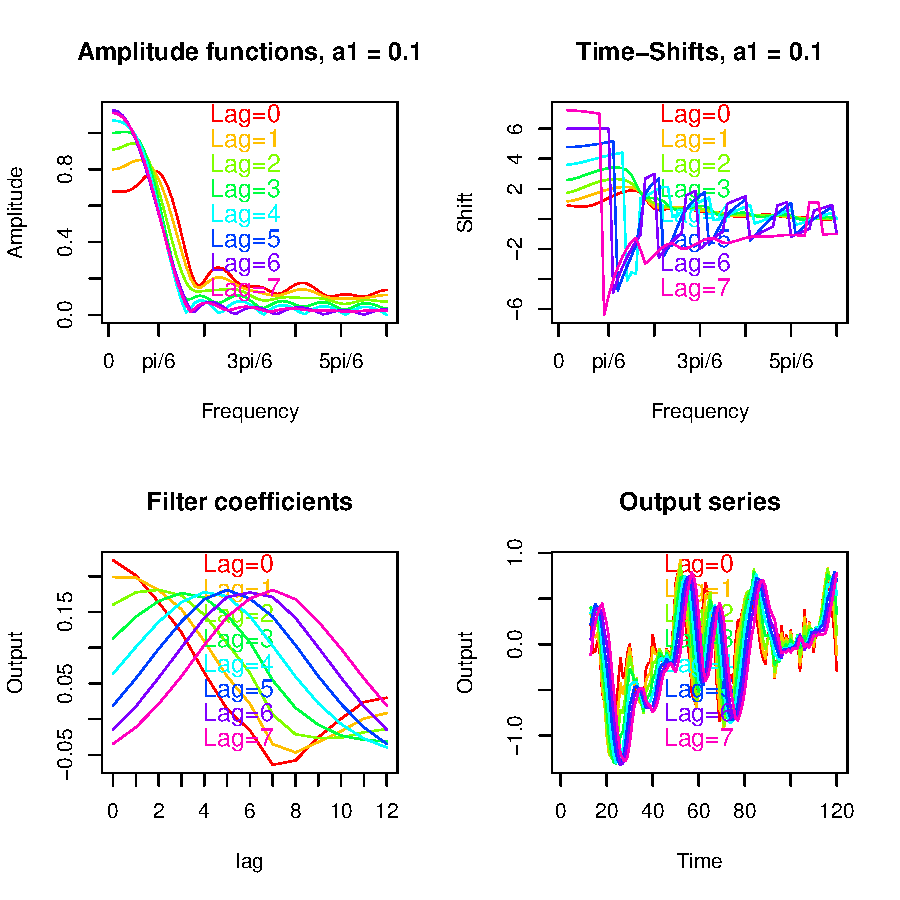
\includegraphics[height=6in, width=6in]{z_dfa_ar1_amp_shift_Lag_0.pdf}\caption{Amplitude (left) and time-shift (right) functions as a function of Lag (rainbow colors) for
  the second process (a1=0.1)\label{z_dfa_ar1_amp_shift_Lag_0}}\end{center}\end{figure}As expected, the time-shift (top-right) increases with increasing Lag (decreasing $h$).
For $Lag=(L-1)/2=6$ the filter is symmetric (see bottom left graph) and therefore
the corresponding time-shift (violet line) is constant\footnote{The shift is constant (flat line) in the passband. The variable shift
in the stopband is an artifact of the Arg-function: the physical shift must be constant
since the filter weights (violet line bottom left
panel) are symmetric.}. In contrast to the symmetric target filter, which is centered about $x_t$, the time-shift of the symmetric $Lag=6$-filter does not vanish because the filter is causal: its coefficients are centered about $x_{t-6}$. We can see that the output series
(bottom-right panel) are shifted accordingly: larger shifts are associated to stronger noise rejection (amplitude closer to zero in the stop-band) and to smoother series. 
\end{enumerate}





\subsection{Filter Vintages}\label{back_uni_rev}


In the GDP table \ref{US_GDP} historical releases are up-dated (revised) when new information becomes available. We could proceed analogously for the above filter-designs: 
\begin{itemize}
\item Assume that in time point $t$ a new observation $x_t$ becomes available. Therefore we can compute a nowcast $\hat{y}_t^0$ of $y_t$ based on the real-time filter $Lag=0$.
\item But we can also improve our previous estimate $\hat{y}_{t-1}^{0}$ of $y_{t-1}$ if the new observation $x_t$ is informative about $y_{t-1}$. For this purpose we can rely on the $Lag=1$ filter and obtain a potentially better estimate $\hat{y}_{t-1}^{-1}$.
\item We do similarly for $\hat{y}_{t-Lag}^{-Lag}$, $Lag>1$: all historical estimates can be up-dated\footnote{The new observation $x_t$ is potentially informative because the target filter is bi-infinite.}.
\end{itemize}
Assume now that we have a sample of length $T$ and define a filter-vintage according to 
\[\hat{y}_{T-t}^{-t}, t=0,...,T-1\]
In each time point $T-t$, the data point $\hat{y}_{T-t}^{-t}$ is the last observation of the output of the $Lag=t$-filter. The series $\hat{y}_{T-t}^{-t}, t=0,...,T-1$ is called a \emph{filter-vintage}. Filter vintages can be arranged in a so-called \emph{filter-vintage triangle}.

\subsubsection{Exercises}
\begin{enumerate}
\item Compute a filter-vintage triangle for each of the above AR(1)-processes. Specifically, use the filters for $Lag=0,...,6$. Note that our maximal Lag-value is six: therefore,  $\hat{y}_{T-t}^{-t},t>6$ is identified with $\hat{y}_{T-t}^{-6}$ i.e. the filter-vintage becomes
\[\hat{y}_{T-t}^{-\min(6,t)}, t=0,...,T-1\]
\begin{Schunk}
\begin{Sinput}
> vintage<-array(dim=c(len,3,len))
> # For each of the three AR(1)-processes We compute the vintage series
> for (i in 1:3)
+ {
+   for (j in L:len)#j<-L
+   {
+     vintage[(j-as.integer(L/2)):j,i,j]<-yhat_Lag[j,i,(as.integer(L/2)+1):1]
+     vintage[1:(j-as.integer(L/2)-1),i,j]<-
+     yhat_Lag[(as.integer(L/2)+1):(j-1),i,as.integer(L/2)+1]
+   }
+ }
> number_vint<-6
\end{Sinput}
\end{Schunk}
\item Compute the last 7 vintages (last 7 columns and rows) for the third process ($a_1=-0.9$),  see table \ref{vintage_triangle}.
\begin{Schunk}
\begin{Sinput}
> # We select the third DGP with a1=-0.9
> i<-3
> vintage_triangle<-vintage[,i,]
> dimnames(vintage_triangle)[[2]]<-paste("Publ. ",1:len,sep="")
> dimnames(vintage_triangle)[[1]]<-paste("Target ",1:len,sep="")
\end{Sinput}
\end{Schunk}
% latex table generated in R 3.3.2 by xtable 1.8-2 package
% Fri Dec 16 15:20:55 2016
\begin{table}[ht]
\centering
\begin{tabular}{rrrrrrrr}
  \hline
 & Publ. 114 & Publ. 115 & Publ. 116 & Publ. 117 & Publ. 118 & Publ. 119 & Publ. 120 \\ 
  \hline
Target 114 & -0.200 & -0.185 & -0.117 & -0.158 & -0.111 & -0.118 & -0.124 \\ 
  Target 115 &  & -0.117 & -0.042 & -0.090 & -0.026 & -0.028 & -0.046 \\ 
  Target 116 &  &  & 0.024 & -0.028 & 0.050 & 0.058 & 0.028 \\ 
  Target 117 &  &  &  & 0.021 & 0.106 & 0.129 & 0.088 \\ 
  Target 118 &  &  &  &  & 0.137 & 0.172 & 0.123 \\ 
  Target 119 &  &  &  &  &  & 0.185 & 0.132 \\ 
  Target 120 &  &  &  &  &  &  & 0.116 \\ 
   \hline
\end{tabular}
\caption{Last few vintages for the AR(1)-process with a1=-0.9: columns correspond to vintages and are indexed
  by corresponding publication dates; rows correspond to revisions of estimates for a fixed historical target date; diagonals correspond to releases: the lowest diagonal corresponds to the first release (real-time filter or nowcast).} 
\label{vintage_triangle}
\end{table}The last column collects the last vintage $\hat{y}_{120-t}^{-t}$ for $t=0,1,...,6$: $\hat{y}_{120}^{0}=0.116$
is the real-time estimate (first release) of the target $y_{120}$ based on data $x_1,...,x_{120}$; $y_{119}^{-1}=0.132$ is the second release of the target $y_{119}$ based on data $x_1,...,x_{120}$ (the output of the $Lag=1$ filter)
and so on. In analogy to table \ref{US_GDP}, the column-date in table
\ref{vintage_triangle} refers to the \emph{publication date} and the row-date refers to the
\emph{target time} i.e. the index $t$ of $y_t$. The initial release
in the first column (publication date 114) is $-0.2$;  the second release
of the same target value $y_{114}$ in the second column is $-0.185$;
the third release in the third column is $-0.117$, and so on. The differences
between the various releases are due to filter-revisions: previous estimates of  $y_{114}$ are up-dated when new information becomes available. The initial release $-0.2$ is up-dated until it reaches its \emph{final} value $-0.124$ in the last column\footnote{Recall that $\hat{y}_{T-t}^{-t}=\hat{y}_{T-t}^{-6}$ if $t>6$ i.e. the estimate of $y_{114}$ won't be revised anymore in later vintages ($T>120$).}.  
\end{enumerate}
\textbf{Remarks}
\begin{itemize}
\item Recall that the data $x_t$ is error-free (fixed). Revisions are solely due to the deployment of the (optimal MSE) filter-sequence.
\item The diagonals of the filter-vintage triangle are the releases: the initial release (first diagonal), the second release (second diagonal), and so on. A diagonal is generated by a fixed filter. Therefore diagonals are stationary time series (assuming stationarity of the data $x_t$).
\item A filter-vintage (a column) is a non-stationary series: the DGP changes because different observations are generated by different filters (at least until the final values are obtained). As an example, the last observation of a vintage is generally `noisier' than earlier observations (because it is based on a causal real-time filter $Lag=0$).
\item Fitting classic models to a vintage series would conflict with model assumptions because the series is non-stationary: the data-quality (noise/delay) worsens towards the sample end due to asymmetry of the underlying filters.
\end{itemize}



\subsection{Tentacle Plot}\label{back_tentacle}




{All} vintages can be collected and plotted in a single graph, called \emph{tentacle plot}. The purpose of a tentacle plot is to reveal the quality of early releases of the filter-vintage by juxtaposing smoothed and real-time estimates. 
\begin{enumerate}
\item Plot the vintages obtained for the three AR(1)-processes \ref{ar1_processes} in the previous section, see fig.\ref{z_vintages}.  
\begin{Schunk}
\begin{Sinput}
> colo<-rainbow(len)
> file = paste("z_vintages.pdf", sep = "")
> pdf(file = paste(path.out,file,sep=""), paper = "special", width = 6, height = 6)
> par(mfrow=c(3,1))
> for (i in 1:3)
+ {
+   ymin<-min(vintage[,i,],na.rm=T)
+   ymax<-max(vintage[,i,],na.rm=T)
+   ts.plot(vintage[,i,L],col=colo[1],ylim=c(ymin,ymax),
+   main=paste("Tentacle plot: vintages and full revision sequence,
+   a1 = ",a_vec[i],sep=""),ylab="Vintages")
+   for (j in (L+1):len)
+   {
+     lines(vintage[,i,j],col=colo[j])
+   }
+   lines(vintage[,i,len],col="red",lwd=2)
+ }
> invisible(dev.off())
\end{Sinput}
\end{Schunk}
\begin{figure}[H]\begin{center}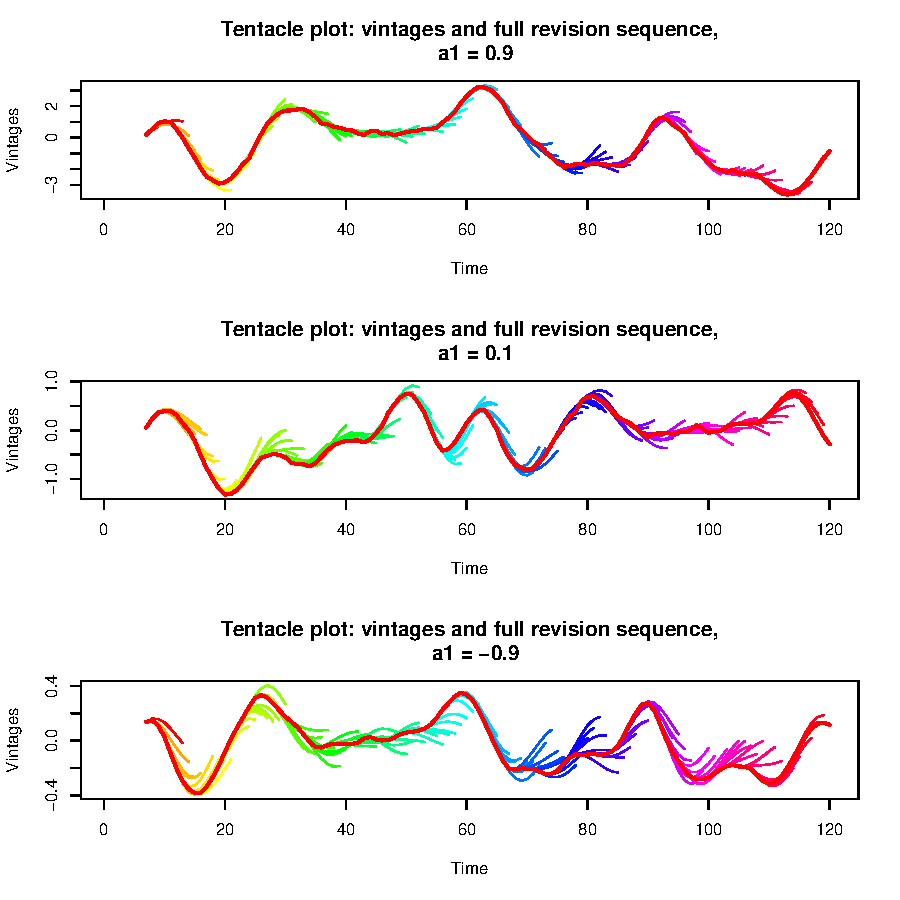
\includegraphics[height=6in, width=6in]{z_vintages.pdf}\caption{Tentacle plot: full historical revision sequence for
  a1=0.9 (top), a1=0.1 (middle) and a1=-0.9 (bottom). Final release is emphasized in bold red\label{z_vintages}}\end{center}\end{figure}The rate of convergence of early releases to their final values and the dynamic pattern of the revisions, in particular in the vicinity of turning points, can be summarized and analyzed conveniently by this graphical tool which provides a backtest of the otherwise unobserved real-time performances of the filter-\emph{sequence}. The plot summarizes intrinsic properties of the filter-\emph{sequence} which are not addressed by previous diagnostic tools (MSEs, amplitude and time-shift functions). A direct comparison of the three tentacle plots confirms, once again, that the signal-extraction task seems less demanding when the data is positively autocorrelated (top graph).

\item we focus attention on the second process ($a_1=0.1$) and emphasize final and initial releases, see fig.\ref{z_vintages_2}. 
\begin{Schunk}
\begin{Sinput}
> file = paste("z_vintages_2.pdf", sep = "")
> pdf(file = paste(path.out,file,sep=""), paper = "special", width = 6, height = 6)
> par(mfrow=c(2,1))
> i<-2
> ymin<-min(vintage[,i,],na.rm=T)
> ymax<-max(vintage[,i,],na.rm=T)
> ts.plot(vintage[,i,L],col=colo[1],ylim=c(ymin,ymax),
+ main="Vintages: full revision sequence and final release (black)",ylab="Vintages")
> for (j in (L+1):len)
+ {
+   lines(vintage[,i,j],col=colo[j])
+ }
> lines(vintage[,i,len],col="black",lwd=2)
> i<-2
> ymin<-min(vintage[,i,],na.rm=T)
> ymax<-max(vintage[,i,],na.rm=T)
> ts.plot(vintage[,i,L],col=colo[1],ylim=c(ymin,ymax),
+ main="Vintages: full revision sequence and real-time initial release (black)",
+ ylab="Vintages")
> for (j in (L+1):len)
+ {
+   lines(vintage[,i,j],col=colo[j])
+ }
> lines(yhat_Lag[,i,1],col="black",lty=1)
> invisible(dev.off())
\end{Sinput}
\end{Schunk}
\begin{figure}[H]\begin{center}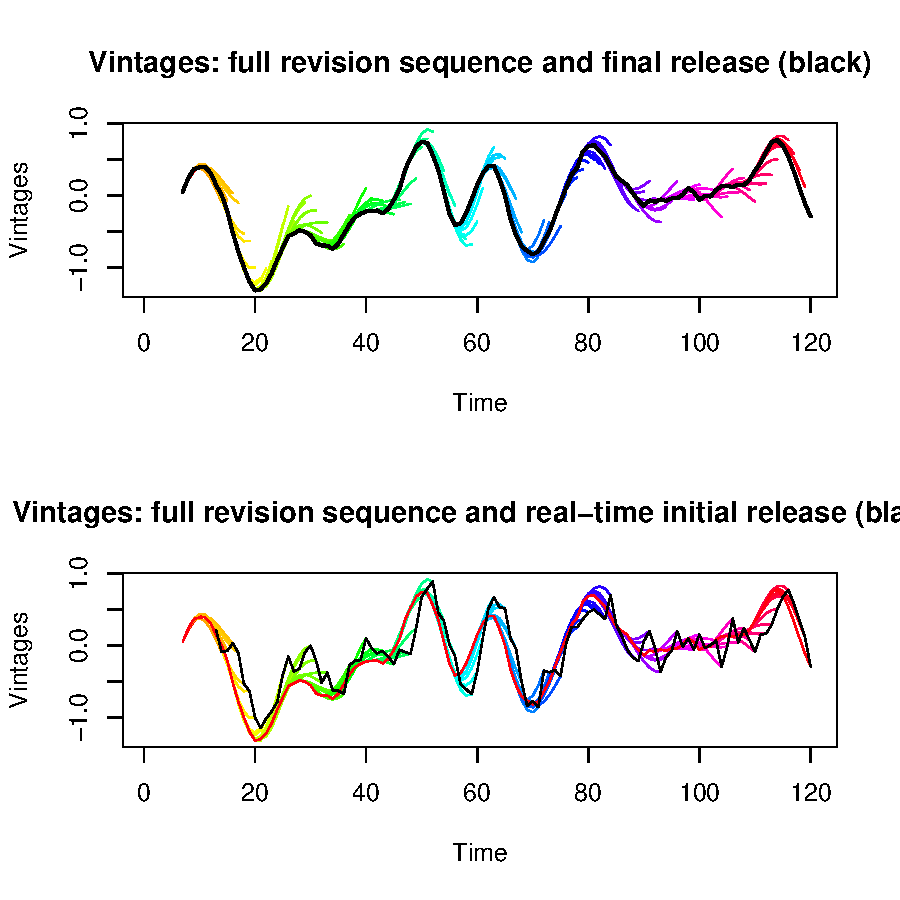
\includegraphics[height=6in, width=6in]{z_vintages_2.pdf}\caption{Vintages: full historical revision sequence in the case of the second  process (a1=0.1)\label{z_vintages_2}}\end{center}\end{figure}Convergence to the final values is achieved after $(L-1)/2=6$ time steps in this particular example. Top and bottom graphs stress final (symmetric filter) and first (concurrent filter) releases, respectively. Linking the end-points of the tentacles in the bottom graph highlights the noisy real-time dynamics as well as the inherent delay towards the sample-end of the filter-vintage: these effects were illustrated in fig.\ref{z_dfa_ar1_amp_shift_Lag_0}, in terms of amplitude and time-shift functions of the one-sided filter. The spreading tentacles at the turning points  suggest that univariate MSE-designs are not ideally suited for inferring growth-breaks in \emph{real time}. A better bivariate filter is proposed in the following section and chapters \ref{ats_sec} and \ref{atsm_sec} propose a generic criterion for tackling `timeliness' and `smoothness' of real-time designs (ATS-trilemma).
\end{enumerate}


\section{Tentacle Plot of the Bivariate Leading Indicator Design}\label{blid}

We here apply the leading indicator design introduced in section \ref{leading_ind}. For simplicity we restrict the analysis to the second process ($a_1=0.1$).
\begin{enumerate}
\item Generate a leading indicator and define the corresponding (3-dim) data matrix.
\begin{Schunk}
\begin{Sinput}
> set.seed(12)
> # Select the AR(1)-process with coefficient 0.1
> i_process<-2
> # Scaling of the idiosyncratic noise
> scale_idiosyncratic<-0.1
> eps<-rnorm(nrow(x))
> indicator<-x[,i_process]+scale_idiosyncratic*eps
> # Data: first column=target, second column=x, 
> #   third column=shifted (leading) indicator
> data_matrix_120<-cbind(x[,i_process],x[,i_process],
+                        c(indicator[2:nrow(x)],indicator[nrow(x)]))
> dimnames(data_matrix_120)[[2]]<-c("target","x","leading indicator")
> head(data_matrix_120)
\end{Sinput}
\begin{Soutput}
         target          x leading indicator
[1,]  0.2207327  0.2207327         0.5695845
[2,]  0.4118676  0.4118676        -1.2625639
[3,] -1.1668894 -1.1668894        -0.5723655
[4,] -0.4803650 -0.4803650        -1.8744734
[5,] -1.6747092 -1.6747092        -0.4511789
[6,] -0.4239493 -0.4239493         1.0278497
\end{Soutput}
\end{Schunk}

\item Compute the DFTs.
\begin{Schunk}
\begin{Sinput}
> # Fully in sample
> insample<-nrow(data_matrix_120)
> # d=0 for stationary series: see default settings
> weight_func<-spec_comp(insample, data_matrix_120, d)$weight_func
\end{Sinput}
\end{Schunk}
\item Estimate optimal (MSE-) filter coefficients as a function of Lag=0,...,6
\begin{Schunk}
\begin{Sinput}
> yhat_Lag_mdfa<-matrix(nrow=len,ncol=L/2+2)
> # Source the default (MSE-) parameter settings
> source(file=paste(path.pgm,"control_default.r",sep=""))
> # Estimate filter coefficients
> for (Lag in 0:((L/2)))
+ {
+   mdfa_obj<-MDFA_mse(L,weight_func,Lag,Gamma)$mdfa_obj 
+ 
+   print(paste("Lag=",Lag," Criterion=",round(mdfa_obj$MS_error,4),sep=""))
+ # Filter coefficients
+   b_mat<-mdfa_obj$b
+ # Compute outputs
+   for (j in L:len)
+     yhat_Lag_mdfa[j,Lag+1]<-sum(apply(b_mat*data_matrix_120[j:(j-L+1),2:3],1,sum))
+ }
\end{Sinput}
\begin{Soutput}
[1] "Lag=0 Criterion=0.0507"
[1] "Lag=1 Criterion=0.0294"
[1] "Lag=2 Criterion=0.0182"
[1] "Lag=3 Criterion=0.0148"
[1] "Lag=4 Criterion=0.0154"
[1] "Lag=5 Criterion=0.0166"
[1] "Lag=6 Criterion=0.0166"
\end{Soutput}
\end{Schunk}
The criterion is minimal at Lag=3 which suggests a rapid convergence of early releases (short tentacles).  
\item Define the vintage triangle.
\begin{Schunk}
\begin{Sinput}
> vintage_mdfa<-matrix(nrow=len,ncol=len)
> # For each of the three AR(1)-processes We compute the vintage series
> for (j in L:len)#j<-len
+ {
+   vintage_mdfa[(j-as.integer(L/2)):j,j]<-yhat_Lag_mdfa[j,(as.integer(L/2)+1):1]
+   vintage_mdfa[1:(j-as.integer(L/2)-1),j]<-
+   yhat_Lag_mdfa[(as.integer(L/2)+1):(j-1),as.integer(L/2)+1]
+ }
\end{Sinput}
\end{Schunk}
\item Generate a tentacle plot, see fig\ref{z_vintages_mdfa}.
\begin{Schunk}
\begin{Sinput}
> file = paste("z_vintages_mdfa.pdf", sep = "")
> pdf(file = paste(path.out,file,sep=""), paper = "special", width = 6, height = 6)
> par(mfrow=c(2,1))
> ymin<-min(vintage_mdfa,na.rm=T)
> ymax<-max(vintage_mdfa,na.rm=T)
> ts.plot(vintage_mdfa[,L],col=colo[1],ylim=c(ymin,ymax),
+ main="Vintages: full revision sequence and final release (black)",ylab="Vintages")
> for (j in (L+1):len)
+ {
+   lines(vintage_mdfa[,j],col=colo[j])
+ }
> lines(vintage_mdfa[,len],col="black",lwd=2)
> ymin<-min(vintage_mdfa,na.rm=T)
> ymax<-max(vintage_mdfa,na.rm=T)
> ts.plot(vintage_mdfa[,L],col=colo[1],ylim=c(ymin,ymax),
+ main="Vintages: full revision sequence and final release (black)",ylab="Vintages")
> for (j in (L+1):len)
+ {
+   lines(vintage_mdfa[,j],col=colo[j])
+ }
> lines(yhat_Lag_mdfa[,1],col="black",lwd=1)
> invisible(dev.off())
\end{Sinput}
\end{Schunk}
\begin{figure}[H]\begin{center}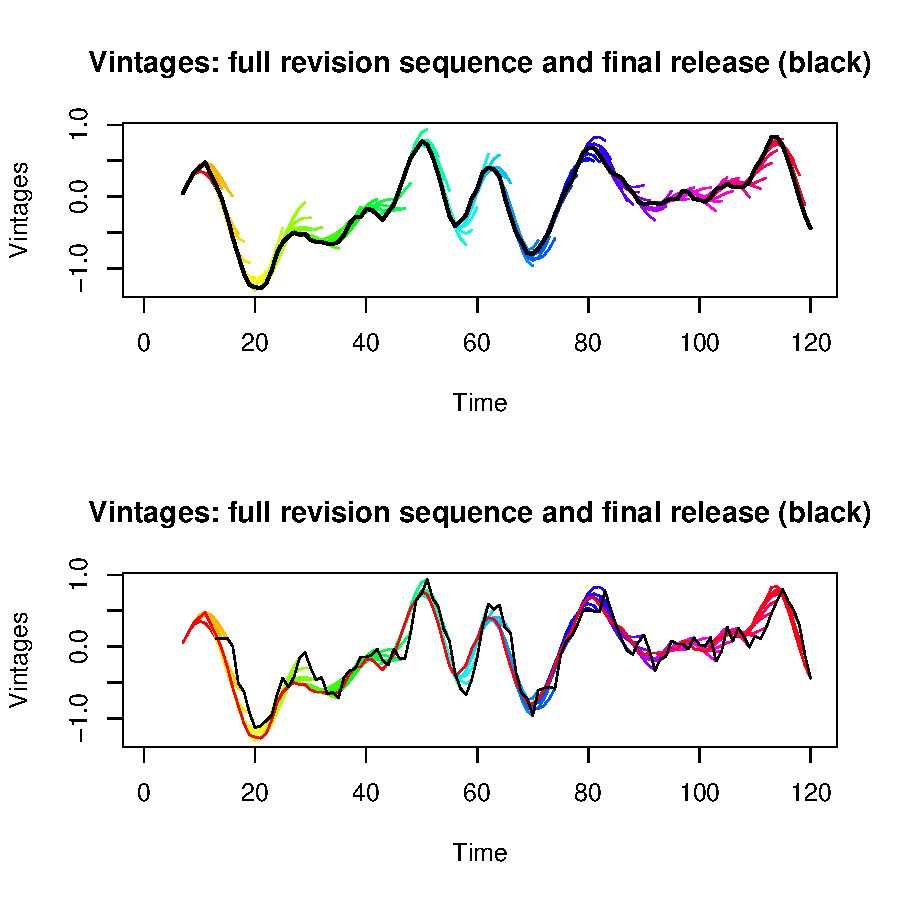
\includegraphics[height=6in, width=6in]{z_vintages_mdfa.pdf}\caption{Vintages: full historical revision sequence in the case of the second process (a1=0.1)\label{z_vintages_mdfa}}\end{center}\end{figure}Visual inspections and comparisons of figs.\ref{z_vintages_mdfa} and \ref{z_vintages_2} (univariate DFA) are more eloquent than a convoluted comparative analysis.

\end{enumerate}

\textbf{Final Remark}
\begin{itemize}
\item When applying a real-time  filter ($Lag=0$) of length $L$ to the data, the output $\hat{y}_{t}^0,t=1,...,L-1$ corresponding to the first $(L-1)$-observations is missing (because the sample starts in $t=1$ i.e. $x_0,x_{-1},x_{-2},...$ are not observed). These missing `initial' values could be obtained in terms of backcasts $\hat{y}_t^{-L+t}, t=1,...,L-1$ (verification of this claim is left as an exercise to the reader).   
\end{itemize}


\section{Summary}

\begin{itemize}
\item We analyzed optimal (time-dependent) filter sequences for tracking a generic target signal at each time point $t=1,...,T$ of a finite sample of length $T$. 
\item We distinguished forecast ($h>0$), nowcast ($h=0$) and backcast ($h<0$) of a generic target: the corresponding estimation problems can be handled by the parameter $Lag=-h$ in the relevant function-calls of DFA and MDFA.
\item All results were based on the assumption of error-free data. Optimal filter design in the presence of data revisions is addressed in chapter \ref{rev_sec}. 
\item We proposed a useful diagnostic tool, the so-called tentacle plot, and benchmarked the bivariate leading-indicator design against the univariate DFA.
\item Pertinence and practical relevance of the proposed filter-sequence is closely linked to the MSE-perspective because the optimization criterion adresses the (mean-square) filter error i.e. the revision error is minimized explicitly. More sophisticated criteria proposed in chapters \ref{ats_sec} and \ref{atsm_sec} will emphasize more specifically \emph{nowcast} and \emph{forecast} applications, instead.
\end{itemize}

%----------------------------------------



\chapter{Filter Constraints}\label{con_sec}

We propose and analyze a set of filter constraints which are deemed to be relevant in applications. Formally, the constraints ensure finiteness of the mean-square filter error in the case of integrated processes\footnote{The constraints address filter characteristics in \emph{frequency zero}. Arbitrary frequencies could be tackled but we did not find any relevant practical application so far.}. Section \ref{i1i2_intr} sets-up the context; a link to integrated processes is proposed in section \ref{pseudo_dft}; a general matrix notation is proposed in section \ref{cons_gen_par}; section \ref{optim_stat} extends the former (unconstrained) MDFA-criterion to the constrained case; finally, section \ref{const_impl_mdfa} illustrates effects (of the constraints) on characteristics of real-time filters.  \\

The constraints proposed in this chapter do not address cross-sectional links, such as required in the presence of cointegration, for example. The relevant multivariate aspects and extensions are proposed in chapter \ref{coint_sec}.

\section{Level and Time-Shift Constraints}\label{i1i2_intr}

\subsection{Level: i1==T}

A first-order (level-) restriction of the coefficients  $b_0,...,b_{L-1}$ of a filter with transfer function $\hat{\Gamma}(\cdot)$ is specified as
\[
\hat{\Gamma}(0)=w
\]
or, equivalently
\begin{eqnarray}\label{cons1}
b_0+b_1+...+b_{L-1}=w
\end{eqnarray}
where $w$ is a constant. For $w:=\Gamma(0)$ the constraint implies that $\hat{\Gamma}(\cdot)$ fits the target $\Gamma(\cdot)$ exactly in frequency zero: typically, then $w=0$ (bandpass or highpass) or $w=1$ (lowpass). If $x_t$ is integrated of order one with a single unit-root in frequency zero, then the proposed restriction ensures a finite mean-square filter error (assuming some mild regularity conditions, see McElroy and Wildi (2014) DFA and Wildi (2005)). Figuratively,  $\hat{y}_t$ tracks the non-stationary level of the target $y_t$. Formally, $\hat{y}_t$ and $y_t$ are cointegrated, with cointegration vector $(1,-1)$.\\

\subsubsection{R Code}

Consider the head of the main MDFA estimation function
\begin{Schunk}
\begin{Sinput}
> head(mdfa_analytic)
\end{Sinput}
\begin{Soutput}
1 function (L, lambda, weight_func, Lag, Gamma, eta, cutoff, i1,             
2     i2, weight_constraint, lambda_cross, lambda_decay, lambda_smooth,      
3     lin_eta, shift_constraint, grand_mean, b0_H0, c_eta, weight_structure, 
4     white_noise, synchronicity, lag_mat, troikaner)                        
5 {                                                                          
6     lambda <- abs(lambda)                                                  
\end{Soutput}
\end{Schunk}
The Boolean $i1$ in the function call of MDFA determines imposition (or not) of the level constraint. The constant $w$ can be set in a vector called $weight\textunderscore constraint$. In a multivariate design one must specify multiple constraints $w^u, u=1,...,m+1$. The restrictions are independent: each time series receives its own weight (cross-sectional dependencies among the constraints are proposed in chapter \ref{coint_sec}). 



\subsection{Time-shift: i2==T}

The time-shift $\hat{\phi}(\omega)=\hat{\Phi}(\omega)/\omega$ of a filter is subject to a singularity in frequency zero. However, the limiting value, as $\omega\to 0$, could be obtained, see section 3.2.3 in \href{http://blog.zhaw.ch/sef/files/2014/10/DFA.pdf}{DFA}:
\begin{eqnarray}
\hat{\phi}(0)&=&\lim_{\omega\to 0}\frac{\hat{\Phi}(\omega)}{\omega}\nonumber\\
&=&\frac{\left.\frac{d}{d\omega}\hat{\Phi}(\omega)\right |_{\omega=0}}{1}\nonumber\\
&=&\frac{\left.\frac{d}{d\omega}\hat{\Gamma}(\omega)\right|_{\omega=0}}{-i\hat{A}(0)}\nonumber\\
&=&\frac{\sum_{j=0}^{L-1}jb_j}{\sum_{j=0}^{L-1}b_j}\label{shift_zero_eq}
\end{eqnarray}
Second and third equalities are obtained from
\begin{eqnarray*}
-i\sum_{j=0}^{L-1}jb_j&=&\left.\frac{d}{d\omega}\hat{\Gamma}(\omega)\right |_{\omega=0}\\
&=&\left.\frac{d}{d\omega}\hat{A}(\omega)\right |_{\omega=0}
\exp(-i\hat{\Phi}(0))-i\hat{A}(0)\exp(-i\hat{\Phi}(0))\left.\frac{d}{d\omega}\hat{\Phi}(\omega)\right |_{\omega=0}\\
&=&-i \hat{A}(0)\left.\frac{d}{d\omega}\hat{\Phi}(\omega)\right |_{\omega=0}
\end{eqnarray*}
The derivative of the amplitude vanishes in zero because the amplitude is a continuous even function
i.e. $\hat{A}(-\omega)=\hat{A}(\omega)$. Note that we implicitly assumed $\hat{\Gamma}(0)>0$ such that $\hat{A}(0)=\hat{\Gamma}(0)=\sum_{j=0}^{L-1}b_j>0$ and thus \ref{shift_zero_eq} applies and is well defined\footnote{As we shall see, the case $\hat{\Gamma}(0)=0$ (highpass or bandpass) does not involve the time-shift in frequency zero. Moreover, the case $\hat{\Gamma}(0)<0$ is generally not practically relevant.}.\\

We are now in a position to formulate a time-shift restriction in frequency zero:
\begin{eqnarray*}
\frac{\sum_{j=0}^{L-1}jb_j}{\sum_{j=0}^{L-1}b_j}=s
\end{eqnarray*}
This expression can be rewritten as
\begin{eqnarray}
\sum_{j=0}^{L-1}(j-s)b_j =0\label{shift_zero_eq_general}
\end{eqnarray}
In practice, a vanishing time-shift $s=0$ in frequency zero, i.e. 
\begin{eqnarray*}
\sum_{j=1}^{L-1}jb_j=0
\end{eqnarray*}
is often a desirable `feature' because turning-points (of the trend) should not be delayed too much. Also, a vanishing time-shift is necessary in order to ensure finiteness of the mean-square filter error if the data is integrated of order two, I(2). 


\subsubsection{R Code}

The Boolean $i2$ in the function call of MDFA determines imposition (or not) of the time-shift constraint. The constant $s$ can be set in a vector called $shift\textunderscore constraint$. In a multivariate design one must specify multiple constraints $s^u, u=1,...,m+1$. The restrictions are independent: each time series receives its own weight (cross-sectional dependencies among the constraints are proposed in chapter \ref{coint_sec}).\\

Since this chapter emphasizes constrained MSE-designs, without customization or regularization, the simpler context-specific $MDFA\textunderscore mse\textunderscore constraint$ function
\begin{Schunk}
\begin{Sinput}
> head(MDFA_mse_constraint)
\end{Sinput}
\begin{Soutput}
1 function (L, weight_func, Lag, Gamma, i1, i2, weight_constraint, 
2     shift_constraint)                                            
3 {                                                                
4     cutoff <- pi                                                 
5     lin_eta <- F                                                 
6     lambda <- 0                                                  
\end{Soutput}
\end{Schunk}
can be used instead of the generic (lengthy) $mdfa\textunderscore analytic$-call.



\subsection{Level and Time-Shift: i1==T,i2==T}

Both constraints can be imposed simultaneously by solving the above expressions for $b_{L-1}$ and $b_{L-2}$:
\begin{eqnarray}\label{cons2}
b_{L-2}&=&(L-1-s)w-(L-1)b_0-(L-2)b_1-...-2b_{L-3}\label{cons2}\\
b_{L-1}&=&(2+s-L)w+(L-2)b_0+(L-3)b_1+(L-4)b_2+...+b_{L-3}\label{cons3}
\end{eqnarray}

\subsection{Exercises: Checking the Formulas}

\begin{enumerate}
\item We verify the filter constraints by a simple number experiment.
\begin{itemize}
\item Define arbitrary filter coefficients $b_0,...,b_3$ and constants $w,s$ and derive $b_4$ and $b_5$ according to \ref{cons2} and \ref{cons3} 
\begin{Schunk}
\begin{Sinput}
> # Filter length
> L<-5
> set.seed(1)
> # The first three coefficients are random numbers
> b<-rnorm(1:(L-2))
> # Define the constants: the following are classical 
> #   restrictions (amplitude is 1 and time shift is zero)
> w<-1
> s<-0
> b<-c(b,(L-1-s)*w-(L-1:(L-2))%*%b,(2+s-L)*w+(L-2:(L-1))%*%b)
\end{Sinput}
\end{Schunk}
\item Verify pertinence of the filter constraints.
\begin{Schunk}
\begin{Sinput}
> # Level constraint
> sum(b)-w
\end{Sinput}
\begin{Soutput}
[1] 8.881784e-16
\end{Soutput}
\begin{Sinput}
> # time-shift constraint
> sum(b*0:(L-1))/sum(b)-s
\end{Sinput}
\begin{Soutput}
[1] 5.051515e-15
\end{Soutput}
\end{Schunk}
Both expressions are (virtually) zero, as desired.
\end{itemize}
\item To be filled: we verify the effects of the filter constraints on amplitude and time-shift functions 
\begin{itemize}
\item univariate: (problem: DFA is cheating (explain why) i.e. one must use MDFA univariate)
\item recompute exercise previous section with i1 and/or i2 imposed with various constraints
\end{itemize}
\end{enumerate}



\section{Filter Constraints, Pseudo-DFT and Pseudo-Periodogram}\label{pseudo_dft}


We briefly link the aforementioned filter restrictions to unit roots of the DGP and we illustrate tracking of the target signals of non-stationary integrated processes by the real time designs (finite mean-square filter error). The treatment is informal, see chapter \ref{int_sec} and Wildi (2005), McElroy and Wildi (2015: DFA paper) for details.

\subsection{Pseudo-DFT and Pseudo-Periodogram}

 Assume that $x_t$ is a realization of an I(1)-process with a single unit-root in frequency zero (typical spectral shape of many economic time series). Then 
\begin{eqnarray*}
\tilde{x}_t&=&x_{t}-x_{t-1}=(1-B)x_t
\end{eqnarray*}
is a stationary process. According to \ref{convolution_dft} (finite sample convolution) we expect that the approximation
\begin{eqnarray*}
\Xi_{\tilde{X}T}(\omega)&\simeq&(1-\exp(-i\omega))\Xi_{TX}(\omega)
\end{eqnarray*}
should be `tight'. Unfortunately, one can show that the gap between left and right-hand sides of the above approximation does not close asymptotically\footnote{The realization of an I(1)-process is not mean-reverting (it is `far from periodic') which conflicts with the intrinsic assumption of the DFT. Fortunately, a very simple linear adjustment of the data, which does not affect its information content, re-establishes perfect equality between both terms in all frequencies (except zero), see Wildi (2005).} and therefore the periodogram of $x_t$ is a biased spectral estimate, see Wildi (2005). For an I(1)-process we consider the so-called pseudo-DFT
\begin{eqnarray*}
\Xi_{TX}^{pseudo}(\omega):=\frac{\Xi_{\tilde{X}T}(\omega)}{1-\exp(-i\omega)},~\omega\neq 0
\end{eqnarray*}
with associated pseudo-periodogram
\[I_{TX}^{pseudo}(\omega)=\left|\Xi_{TX}^{pseudo}(\omega)\right|^2,~\omega\neq 0\]
where $\Xi_{\tilde{X}T}(\omega)$ relies on first differences $\tilde{x}_t$ of the data. The pseudo-periodogram is an unbiased estimate of the pseudo-spectral density. The pseudo-DFT (pseudo-periodogram) is defined in all frequencies except $\omega=0$. 



\subsection{First Order Constraint}\label{first_order_cons}

Consider an extension of the stationary (univariate) DFA-criterion \ref{dfa_ms}
\begin{eqnarray}
&&\left.\frac{2\pi}{T}\sum_{k=-[T/2]}^{[T/2]}\left|\Delta\Gamma(\omega_k) \right|^2I_{TX}^{pseudo}(\omega_k)\right|_{\Gamma(0)=\hat{\Gamma}(0)}\nonumber\\
&=&\left.\frac{2\pi}{T}\sum_{k=-[T/2]}^{[T/2]}\frac{\left|\Delta\Gamma(\omega_k) \right|^2}{|1-\exp(-i\omega_k)|^2}I_{T\tilde{X}}(\omega_k)\right|_{\Gamma(0)=\hat{\Gamma}(0)}\to\min_{\mathbf{b}} \label{dfa_ms_i}
\end{eqnarray}
where the original periodogram has been replaced by the unbiased pseudo-periodogram. Interestingly, the singularity in frequency zero can be adressed by imposing the level constraint
\[\Delta\Gamma(0)=\Gamma(0)-\hat{\Gamma}(0)=0\]
i.e. the limit 
\[
\left.\lim_{\omega\to 0}\frac{\left|\Delta\Gamma(\omega) \right|^2}{|1-\exp(-i\omega)|^2}I_{T\tilde{X}}(\omega)\right|_{\Gamma(0)=\hat{\Gamma}(0)}
\]
exists. More precisely, assuming a mild set of regularity assumptions, one can show that the coefficients of the filter 
\begin{equation}\label{def_Gamma_t}
\tilde{\Gamma}(\omega):=\left.\displaystyle{\frac{\Delta\Gamma(\omega) }{1-\exp(-i\omega)}}\right|_{\Gamma(0)=\hat{\Gamma}(0)}
\end{equation} 
are well-defined and converge at a suitable rate towards zero with increasing/decreasing lags, see Wildi (2005). Therefore, consider 
\[\Gamma(\omega)-\hat{\Gamma}(\omega)=\tilde{\Gamma}(\omega)(1-\exp(-i\omega))\]
We infer that the difference of target and real-time filters, on the left side, can be factored into a well-defined MA-filter $\tilde{\Gamma}(\omega)$ and a first difference operator. Our estimation problem can then be stated in (at least) two equivalent ways:
\begin{itemize}
\item Apply the filter with transfer function $\Gamma(\omega)-\hat{\Gamma}(\omega)$ to the non-stationary data $x_t$ and determine `optimal' filter coefficients of $\hat{\Gamma}(\omega)$.
\item Apply the filter with transfer function $\tilde{\Gamma}(\omega)$ to the stationary data $\tilde{x}_t$ and determine `optimal' filter coefficients of $\hat{\Gamma}(\omega)$ (these coefficients enter into $\tilde{\Gamma}(\omega)$ via \ref{def_Gamma_t}).  
\end{itemize}
In the latter case, we are back to the stationary case discussed in chapter \ref{mse_sec} (except that we have to impose a filter constraint). In particular
\begin{eqnarray*}
\left.\frac{2\pi}{T}\sum_{k=-[T/2]}^{[T/2]}\left|\tilde{\Gamma}(\omega_k) \right|^2I_{T\tilde{X}}(\omega_k)\right|_{\Gamma(0)=\hat{\Gamma}(0)} 
\end{eqnarray*}
is a superconsistent estimate of the (sample) mean-square filter error and therefore criterion \ref{dfa_ms_i} is pertinent. \\


We conclude that the proposed level-constraint $\sum_{k=0}^{L-1}b_{k}=\Gamma(0)$ ensures existence and pertinence of the optimization criterion \ref{dfa_ms_i}. Moreover, the filter error $y_t-\hat{y}_t$ is stationary i.e. the mean-square filter error is finite\footnote{An extension to for/backcasting is straightforward by imposing $\sum_{k=h}^{L-1+h}b_{kh}=\Gamma(0)$.}. If $\Gamma(0)>0$ and if $\Gamma(\omega)$ is sufficiently regular in a vicinity of $\omega=0$, then the non-stationary target $y_t$ and the non-stationary finite sample estimate $\hat{y}_t$ are cointegrated with cointegration vector $(1,-1)$. If $\Gamma(0)=0$ and if $\Gamma(\omega)$ is sufficiently regular in a vicinity of $\omega=0$, then both the target $y_t$ as well as the finite sample estimate $\hat{y}_t$ are stationary. 




\subsection{Second Order Constraint}\label{socco}

We here assume that $x_t$ is a realization of an I(2)-process. Then the pseudo-DFT (-periodogram) becomes
\begin{eqnarray}
\Xi_{TX}^{pseudo}(\omega)&:=&\frac{\Xi_{\tilde{X}T}(\omega)}{(1-\exp(-i\omega))^2},~\omega\neq 0\nonumber\\
I_{TX}^{pseudo}(\omega)&=&\left|\Xi_{TX}^{pseudo}(\omega)\right|^2,~\omega\neq 0\label{pseudo_per_i2}
\end{eqnarray}
where 
\begin{eqnarray*}
\tilde{x}_t&=&(1-B)^2x_t
\end{eqnarray*}
are the stationary second-order differences of the data. Consider the following optimization criterion 
\begin{eqnarray}
&&\left.\frac{2\pi}{T}\sum_{k=-[T/2]}^{[T/2]}\left|\Delta\Gamma(\omega_k) \right|^2I_{TX}^{pseudo}(\omega_k)\right|_{\Delta\Gamma(0)=\Delta\Gamma^{(1)}(0)=0}\nonumber \\
&=&\left.\frac{2\pi}{T}\sum_{k=-[T/2]}^{[T/2]}\frac{\left|\Delta\Gamma(\omega_k) \right|^2}{|1-\exp(-i\omega_k)|^4}I_{T\tilde{X}}(\omega_k)\right|_{\Delta\Gamma(0)=\Delta\Gamma^{(1)}(0)=0}\to\min_{\mathbf{b}}\label{sos_rhs}
\end{eqnarray}
where we impose first- and second-order constraints
\begin{eqnarray*}
\Delta\Gamma(0)&=&0\\
\Delta\Gamma^{(1)}(0)&=&\left.\frac{d (\Gamma(\omega)-\hat{\Gamma}(\omega))}{d\omega}\right|_{\omega=0}=0
\end{eqnarray*}
Note that \(\left.d
\Gamma(\omega)/d\omega\right|_{\omega=0}=0\) in the second order-constraint, by symmetry of the target filter, (even function) so that we must impose a vanishing derivative of $\hat{\Gamma}(\cdot)$ in $\omega=0$ for the constraint to hold. We first consider the case $ |\Gamma(0)|>0$ (lowpass target). Let
\[\hat{\Gamma}(\omega)=\hat{A}(\omega)\exp(-i\hat{\Phi}(\omega))\]
so that
\begin{eqnarray}\label{dd0}
\left.\frac{d\hat{\Gamma}(\omega)}{d\omega}\right|_{\omega=0}&=&
\left.\frac{d\hat{A}(\omega)}{d\omega}\right|_{\omega=0}\exp(-i\hat{\Phi}(0))-
i\hat{A}(0)\exp(-i\hat{\Phi}(0))\left.\frac{d\hat{\Phi}(\omega)}{d\omega}\right|_{\omega=0}\label{dd0_dodo}\\
&=&-i\hat{A}(0)\left.\frac{d\hat{\Phi}(\omega)}{d\omega}\right|_{\omega=0}\label{dd0}
\end{eqnarray}
where \(\left.d\hat{A}(\omega)/d\omega\right|_{\omega=0}=0\)
by symmetry of the amplitude function\footnote{Note that $\hat{A}(0)>0$ (level constraint) and therefore the derivative exists.} (even function). Since  \(\hat{A}(0)=|\Gamma(0)|>0\) (first order constraint), the derivative in (\ref{dd0}) vanishes in \(\omega=0\)
if and only if
\begin{eqnarray}\label{soar}
\left.\frac{d\hat{\Phi}(\omega)}{d\omega}\right|_{\omega=0}=\lim_{h\to
0}\frac{\hat{\Phi}(h)-\hat{\Phi}(0)}{h}=\hat{\phi}(0)=0
\end{eqnarray}
where we used the fact that the phase function vanishes in 
\(\omega=0\). We infer that both the first order level as well as the second-order time-shift constraints are necessary in order to cancel the second-order singularity in \ref{sos_rhs} if $|\Gamma(0)|>0$\footnote{Intuitively the vanishing time-shift is necessary because the slope (first difference) of the data diverges asymptotically.}. On the other hand, if \(\Gamma(0)=0\) (bandpass, highpass) then $\hat{A}(0)=0$ (first order level constraint). Therefore the right-hand side of \ref{dd0_dodo} vanishes iff 
\(\left.d\hat{A}(\omega)/d\omega\right|_{\omega=0}=0\). However, the last equality together with $\hat{A}(0)=0$ implies that the zero of the amplitude function must be of order two in frequency zero, because $\hat{A}(\cdot)$ is an even function\footnote{A graphical illustration of the double-zero in frequency zero is obtained in fig.\ref{z_HP_us_real_log_gdp_hp_diff__gap_amp}, chapter \ref{rep_sec}: the bottom-right panel (double-zero in frequency-zero) is to be contrasted with the bottom-left panel (single zero in frequency zero).}. The same argument applies to $\Gamma(\cdot)$ which is an even function, too. Therefore, both filter outputs $y_t$ and $\hat{y}_t$ are stationary and therefore the filter-error is stationary too i.e. the mean-square filter error is finite, irrespective of the time-shift of the real-time filter.\\

In analogy to the previous section, one can show that the coefficients of the filter 
\begin{equation}\label{til_til_digg_gamma}
\left.\tilde{\Gamma}(\omega):=\displaystyle{\frac{\Delta\Gamma(\omega) }{(1-\exp(-i\omega))^2}}\right|_{\Delta\Gamma(0)=\Delta\Gamma^{(1)}(0)=0}
\end{equation} 
are well defined and converge at a suitable rate towards zero with increasing lag, see Wildi (2005). As a consequence,  our estimation problem can be stated in (at least) two equivalent ways:
\begin{itemize}
\item Apply the filter with transfer function $\Gamma(\omega)-\hat{\Gamma}(\omega)$ to the non-stationary data $x_t$ and determine `optimal' filter coefficients of $\hat{\Gamma}(\omega)$.
\item Apply the filter with transfer function $\tilde{\Gamma}(\omega)$ to the stationary data $\tilde{x}_t$ and determine `optimal' filter coefficients of $\hat{\Gamma}(\omega)$ (these coefficients enter into $\tilde{\Gamma}(\omega)$ via \ref{til_til_digg_gamma}).  
\end{itemize}
In the latter case, we are back to the stationary case discussed in chapter \ref{mse_sec} (except that we have to impose a double filter constraint). In particular
\begin{eqnarray*}
\left.\frac{2\pi}{T}\sum_{k=-[T/2]}^{[T/2]}\left|\tilde{\Gamma}(\omega_k) \right|^2I_{T\tilde{X}}(\omega_k)\right|_{\Delta\Gamma(0)=\Delta\Gamma^{(1)}(0)=0}
\end{eqnarray*}
is a superconsistent estimate of the (sample) mean-square filter error and therefore criterion \ref{sos_rhs} is pertinent. In particular, the filter error $y_t-\hat{y}_t$ is stationary. If $\Gamma(0)>0$ and if $\Gamma(\omega)$ is sufficiently regular in $\omega=0$ then the non-stationary target $y_t$ and the non-stationary estimate $\hat{y}_t$ are cointegrated with cointegration vector $(1,-1)$. If $\Gamma(0)=0$ and if $\Gamma(\omega)$ is sufficiently regular in $\omega=0$ then both the target $y_t$ and the estimate $\hat{y}_t$ are stationary\footnote{Assuming mild regularity restrictions, the zero of $\Gamma(\omega)$ must be of second order because the function is even (symmetric around zero).}.  


\section{General Parametrization}\label{cons_gen_par}

\subsection{Caveats}

The particular parametrization of the filter constraints in terms of $b_{L-1}$ and $b_{L-2}$ in \ref{cons2} and \ref{cons3} is to some extent arbitrary. Indeed, we could have selected $b_0$ and $b_1$, instead. Of course, our particular choice does not affect the estimation result, at least as long as the coefficients are otherwise freely determined. Unfortunately, the regularization features to be introduced in chapter \ref{reg_sec} conflict with this assumption. Therefore we here propose a more general approach.



\subsection{Nowcasting, Forecasting and Smoothing}\label{implement}


We want to estimate $y_{T+h}$ for $h>0$ (forecasting), $h=0$ (nowcasting) or $h< 0$ (backcasting), given data $x_T,x_{T-1},...,x_{T-(L-1)}$, see section \ref{for_now_smo}. If $h=0$ (nowcasting) then imposing a vanishing time shift ($s=0$) means that $\hat{y}_t$ and $y_t$ are `synchronized' (at least in frequency zero). If $h\neq 0$, then the synchronization should apply between $\hat{y}_{t-h}^h$ and $y_t$ i.e. the vanishing time-shift should apply to the \emph{shifted} output signal. Relying on  \ref{shift_zero_eq} we obtain:
\begin{eqnarray*}
\hat{\phi}(0)&=&\frac{\sum_{j=h}^{L-1+h}jb_{jh}}{\sum_{j=h}^{L-1+h}b_{jh}}
\end{eqnarray*}
and the time-shift constraint \ref{shift_zero_eq_general} becomes
\begin{eqnarray}
\sum_{j=h}^{L-1+h}(j-s)b_{jh} =0\label{cons11s}
\end{eqnarray}
The level constraint is `as usual'
\begin{eqnarray}\label{cons1s}
b_{hh}+b_{h+1,h}+...+b_{h+(L-1),h}=w
\end{eqnarray}

\subsection{Implementing the Filter Constraints}

As discussed, any single coefficient $b_{jh}$ (single constraint) or any pair of coefficients (both constraints imposed) could be isolated out of the above equations for implementing the constraint(s). In order to avoid conflicts with later regularization features, see chapter \ref{reg_sec}, we here select $b_{max(0,h),h}$ (single constraint) or $b_{max(0,h),h},b_{max(0,h)+1,h}$ (both constraints imposed) as \emph{natural candidate(s)}. For $h\geq 0$ (nowcast/forecast) these are $b_{hh}, b_{h+1,h}$ i.e. the coefficients assigned to the last data points $x_T,x_{T-1}$, which are likely to be most informative for $y_{T+h}$. For $h<0$ (backcast) these are $b_{0h}$, $b_{1h}$ i.e the coefficient assigned to $x_{T-|h|}$ and $x_{T-|h|-1}$ which are likely to be most informative for $y_{T-|h|}$  (recall that the backcast filter is `centered' about $x_{T-|h|}$).








\subsection{Matrix Notation}\label{matrix_notation_constraints}

For notational ease we now drop the index $h$ from the subscripts i.e. we write $b_j$ instead of $b_{jh}$. The proposed filter constraints can then be re-written in the generic form
\begin{eqnarray}\label{cons5s}
\mathbf{b}&=&\mathbf{R b_{f}}+\mathbf{c}
\end{eqnarray}
where $\mathbf{b_f}$ is the vector of freely determined coefficients. We now specify the right-hand side of this equation for each of the three relevant cases: i1=T, i2=F (simple level-constraint), i1=F, i2=T (simple time-shift constraint) and i1=i2=T (both constraints imposed).  


\subsubsection{The case $i1<-T$, $i2<-F$}

We consider a general multivariate framework with $m+1$ explanatory variables $(x_t,w_{1t},...,w_{mt})$. In this case we obtain
\begin{eqnarray*}
b_{\max(0,h)}^u=w^u-\sum_{k=h,k\not=0}^{h+L-1}b_k^u
\end{eqnarray*}
where the index $u=0,...,m$ runs across series ($u=0$ corresponds to $x_t$). \\



The entries in \ref{cons5s} become
\begin{eqnarray}
\mathbf{R}&=&\left(\begin{array}{cccc}
\mathbf{C}&0&...&0\\
0&\mathbf{C}&...&0\\
:::\\
0&0&...&\mathbf{C}
\end{array}\right)\label{app1}\\
\mathbf{C}&=&\left(\begin{array}{cccccc}
1&0&0&...&0&0\\
0&1&0&...&0&0\\
:::\\
-1&-1&-1&...&-1&-1\\
:::\\
0&0&0&...&1&0\\
0&0&0&...&0&1
\end{array}\right)\label{app2}\\
\mathbf{c}'&=&(0,...,0,w^0,0,...,0~||~0,...,0,w^1,0,...,0~||~...~||0,...,0,w^m,0,...,0)\nonumber\\
\mathbf{b_f}'&=&(b_{h}^0,...,b_{-1}^0,b_1^0,...,b_{h+L-1}^0~||~b_{h}^1,...,b_{-1}^1,b_1^1,...,b_{h+L-1}^1~||~...~||~b_{h}^m,...,b_{-1}^m,b_1^m,...,b_{h+L-1}^m)\nonumber
\end{eqnarray}
The vector of -1's in $\mathbf{C}$ is in row-position $\max(0,-h)+1$ whereas the constant $w^u$ ($u=0,...,m$) in $\mathbf{c}$ is in position $u*(L-1)+\max(0,-h)+1$. The vector $\mathbf{b_f'}$ collects all freely determined parameters (thus $b_0^u$ is missing) whereas $\mathbf{b}$ collects all coefficients: the former vector is used for optimization and the latter is required for filtering. 




\subsubsection{The case $i1<-F$, $i2<-T$}


We consider a simple time-shift constraint without level requirement\footnote{This case would be quite unusual in a classic model-based approach because imposition of the second-order constraint would require the first-order constraint as a prerequisite.} and we first assume $s\neq 0$ and $h<0$ (backcast). From \ref{cons11s} we obtain
\[
-sb_0^u=-(h-s)b_{h}^u-(h+1-s)b_{h+1}^u-...-(-1-s)b_{-1}^u-(1-s)b_1-(2-s)b_2^u-...-(h+L-1-s)b_{h+L-1}^u
\]
or equivalently
\[
b_0^u=\frac{(h-s)b_{h}^u+(h+1-s)b_{h+1}^u+...+(-1-s)b_{-1}^u+(1-s)b_1+(2-s)b_2^u+...+(h+L-1-s)b_{h+L-1}^u}{s}
\]
Such that
\begin{eqnarray}\label{cons6s}
\mathbf{C}_{h<0}&=&\left(\begin{array}{ccccccccc}
1&0&0&...&...&...&...&0&0\\
0&1&0&...&...&...&...&0&0\\
:::\\
\displaystyle{\frac{h-s}{s}}&\displaystyle{\frac{h+1-s}{s}}&\displaystyle{\frac{h+2-s}{s}}&...&\displaystyle{\frac{-1-s}{s}}&\displaystyle{\frac{1-s}{s}}&\displaystyle{\frac{2-s}{s}}&...&\displaystyle{\frac{h+L-1-s}{s}}\\
:::\\
0&0&0&...&...&...&...&1&0\\
0&0&0&...&...&...&...&0&1
\end{array}\right)\\
\mathbf{c}_{h<0}'&=&\mathbf{0}\\
\nonumber\\
\mathbf{b_f}'&=&(b_{h}^0,...,b_{-1}^0,b_1^0,...,b_{h+L-1}^0~||~b_{h}^1,...,b_{-1}^1,b_1^1,...,b_{h+L-1}^1~||~...~||~b_{h}^m,...,b_{-1}^m,b_1^m,...,b_{h+L-1}^m)\nonumber
\end{eqnarray}
The vector $\left(\displaystyle{\frac{h-s}{s}},...,\displaystyle{\frac{h+L-1-s}{s}}\right)$ in $\mathbf{C}_{h<0}$ is in row-position $-h+1$. The vector $\mathbf{b_f}$ collects the freely determined coefficients: all coefficients except $b_0^u$.\\

The case $h=0$ (nowcast) is handled by
\begin{eqnarray*}%\label{cons6s}
\mathbf{C}_{h=0}&=&\left(\begin{array}{cccc}
\displaystyle{\frac{1-s}{s}}&\displaystyle{\frac{2-s}{s}}&...&\displaystyle{\frac{L-1-s}{s}}\\
1&0&...&0\\
:::\\
0&0&...&1
\end{array}\right)\nonumber\\
\mathbf{c}_{h=0}'&=&\mathbf{0}\\
\nonumber\\
\mathbf{b_f}'&=&(b_1^0,...,b_{L-1}^0~||~b_1^1,...,b_{L-1}^1~||~...~||~b_1^m,...,b_{L-1}^m)\nonumber\end{eqnarray*}
and the case $h>0$ (forecast) corresponds to 
\[
(h-s)b_h^u=-(h+1-s)b_{h+1}^u-(h+2-s)b_{h+2}^u-...-(h+L-1-s)b_{h+L-1}^u
\]
or, equivalently
\[
b_h^u=\frac{-(h+1-s)b_{h+1}^u-(h+2-s)b_{h+2}^u-...-(h+L-1-s)b_{h+L-1}^u}{h-s}
\]
We obtain
\begin{eqnarray*}%\label{cons6s}
\mathbf{C}_{h>0}&=&\left(\begin{array}{cccc}
-\displaystyle{\frac{h+1-s}{h-s}}&-\displaystyle{\frac{h+2-s}{h-s}}&...&-\displaystyle{\frac{h+L-1-s}{h-s}}\\
1&0&...&0\\
:::\\
0&0&...&1
\end{array}\right)\nonumber\\
\mathbf{c}_{h>0}'&=&\mathbf{0}\\
\nonumber\\
\mathbf{b_f}'&=&(b_{h+1}^0,...,b_{h+L-1}^0~||~b_{h+1}^1,...,b_{h+L-1}^1~||~...~||~b_{h+1}^m,...,b_{h+L-1}^m)\nonumber\end{eqnarray*}
Note that we implicitly assumed $h-s\neq 0$ in the above derivation. Otherwise we would have to isolate $b_{h+1}$ instead of $b_h$ (left as an exercise to the reader). Recall, also, that we assumed $s\neq 0$ in the case $h\leq 0$: if $s=0$ then we isolate $b_1$, instead of $b_0$, in the above expressions\footnote{If $s=0$ then, obviously, $1-s\neq 0$ and therefore the quotients will be defined.} (left as an exercise to the reader). 



\subsubsection{The case $i1<-T$, $i2<-T$}

As in the previous section, we first tackle the backcast-problem: $h<0$. Solving for $b_0^u$ and $b_1^u$ in \ref{cons11s} and \ref{cons1s} leads to
\begin{eqnarray*}%\label{cons2s}
b_{1}^u&=&s^uw^u-hb_{h}^u-(h+1)b_{h+1}^u-...-(-1)b_{-1}^u-0-2b_{2}^u-3b_{3}^u-...-(h+L-1)b_{h+L-1}^u\nonumber\\
b_{0}^u&=&w^u(1-s^u)+(h-1)b_{h}^u+hb_{h+1}^u+...+(-2)b_{-1}^u+b_{2}^u+2b_3^u+...+(L-2+h)b_{L-1+h}^u\nonumber%\label{cons3s}
\end{eqnarray*}
We obtain
\begin{eqnarray}\label{cons77s}
\mathbf{C}_{h<0}&=&\left(\begin{array}{ccccccccc}
1&0&0&...&&&&0&0\\
0&1&0&...&&&&0&0\\
:::\\
h-1&h&h+1&...&-2&1&2&...&(L-2+h)\\
-h&-(h+1)&-(h+2)&...&1&-2&-3&...&-(h+L-1)\\
:::\\
0&0&0&...&&&&1&0\\
0&0&0&...&&&&0&1
\end{array}\right)\\
\mathbf{c}_{h<0}'&=&(0,...,0,w^0(1-s^0),s^0w^0,0,...,0~||~0,...,0,w^1(1-s^1),s^1w^1,0,...,0~||~...~||\\
&&0,...,0,w^m(1-s^m),s^mw^m,0,...,0)\nonumber\\
\mathbf{b_f}'&=&(b_{-h}^0,...,b_{-1}^0,b_2^0,...,b_{L-1-h}^0~||~b_{-h}^1,...,b_{-1}^1,b_2^1,...,b_{L-1-h}^1~||~...~||~b_{-h}^m,...,b_{-1}^m,b_2^m,...,\\
&&b_{L-1-h}^m)\nonumber
\end{eqnarray}
The non-trivial weighting-vectors in $\mathbf{C}_{h<0}$ are located in row-positions $-h+1$ and $-h+2$ whereas the constants $w^u(1-s^u)$ and $s^uw^u$ in $\mathbf{c}_{h<0}$ are to be found in positions $u*(L-2)-h+1$ and $u*(L-2)-h+2$, respectively. Note that both $b_0^u$ and $b_1^u$ are now missing in the vector of freely determined coefficients $\mathbf{b_f}$. \\


For $h=0$ we obtain
\begin{eqnarray}\label{cons77s}
\mathbf{C}_{h=0}&=&\left(\begin{array}{ccccccccc}
1&2&...&(L-2)\\
-2&-3&...&-(L-1)\\
1&&0&0\\
:::\\
0&...&0&1
\end{array}\right)\\
\mathbf{c}_{h=0}'&=&w^0(1-s^0),s^0w^0,0,...,0~||~w^1(1-s^1),s^1w^1,0,...,0~||~...~||w^m(1-s^m),s^mw^m,0,...,0)\nonumber\\
\mathbf{b_f}'&=&(b_2^0,...,b_{L-1}^0~||~b_2^1,...,b_{L-1}^1~||~...~||~b_2^m,...,b_{L-1}^m)\nonumber
\end{eqnarray}
Finally, for $h>0$ the constraints become
\begin{eqnarray*}%\label{cons2s}
(h+1)b_{h+1}^u&=&s^uw^u-(h+2)b_{h+2}^u-(h+3)b_{h+3}-...-(h+L-1)b_{h+L-1}^u\nonumber\\
hb_{h}^u&=&w^u(1-s^u)+(h+1)b_{h+2}^u+(h+2)b_{h+3}^u+...+(h+L-2)b_{h+L-1}^u\nonumber%\label{cons3s}
\end{eqnarray*}
or, equivalently
\begin{eqnarray*}%\label{cons2s}
b_{h+1}^u&=&\frac{s^uw^u-(h+2)b_{h+2}^u-(h+3)b_{h+3}-...-(h+L-1)b_{h+L-1}^u}{h+1}\nonumber\\
b_{h}^u&=&\frac{w^u(1-s^u)+(h+1)b_{h+2}^u+(h+2)b_{h+3}^u+...+(h+L-2)b_{h+L-1}^u}{h}\nonumber%\label{cons3s}
\end{eqnarray*}
so that
\begin{eqnarray*}%\label{cons6s}
\mathbf{C}_{h> 0}&=&\left(\begin{array}{ccccc}
\displaystyle{\frac{h+1}{h}}&\displaystyle{\frac{h+2}{h}}&\displaystyle{\frac{3}{h}}&...&\displaystyle{\frac{h+L-2}{h}}\\
-\displaystyle{\frac{h+2}{h+1}}&-\displaystyle{\frac{h+3}{h+1}}&-\displaystyle{\frac{h+4}{h+1}}&...&-\displaystyle{\frac{h+L-1}{h+1}}\\
1&0&0&...&0\\
0&1&0&...&0\\
:::\\
0&0&0&...&1
\end{array}\right)\nonumber\\
\mathbf{c}_{h> 0}'&=&(\displaystyle{\frac{w^0(1-s^0)}{h}},\displaystyle{\frac{s^0w^0}{h+1}},0,...,0~||\displaystyle{\frac{w^1(1-s^1)}{h}},\displaystyle{\frac{s^1w^1}{h+1}},0,...,0~||~...~||\\
&&\displaystyle{\frac{w^m(1-s^m)}{h}},\displaystyle{\frac{s^mw^m}{h+1}},0,...,0)\nonumber\\
\mathbf{b_f}'&=&(b_{-h}^0,...,b_{-1}^0,b_2^0,...,b_{L-1-h}^0~||~b_{-h}^1,...,b_{-1}^1,b_2^1,...,b_{L-1-h}^1~||~...~||~b_{-h}^m,...,b_{-1}^m,b_2^m,...,b_{L-1-h}^m)\nonumber
\end{eqnarray*}
Obviously, all expressions on the right-hand side of \ref{cons5s} depend on i1, i2 as well as on $h$ but for notational simplicity we refrain from attaching a cumbersome triple index to them. 



 
\section{Constrained Optimization}\label{optim_stat}

\subsection{Generalized Criterion}

Optimal constrained filter coefficients can be obtained by plugging \ref{cons5s} into \ref{regms} and by taking derivatives 
\begin{eqnarray*}
d/d\mathbf{b_f}~\textrm{Criterion}&=&d/d\mathbf{b_f}~(\mathbf{Y_{\textrm{rot}}-X_{\textrm{rot}}\left(\mathbf{R b_{f}}+\mathbf{c}\right)})'(\mathbf{Y_{\textrm{rot}}-X_{\textrm{rot}}\left(\mathbf{R b_{f}}+\mathbf{c}\right)})\nonumber\\
&=&-2(\mathbf{Y_{\textrm{rot}})'\Re\left(X_{\textrm{rot}}\right)R-
2\Re\bigg\{\mathbf{(X_{\textrm{rot}}c)'(X_{\textrm{rot}}R)}\bigg\}
+2b_f'\Re\bigg\{(X_{\textrm{rot}}R)'X_{\textrm{rot}}R\bigg\}}
\end{eqnarray*}
The \emph{constrained }solution is obtained by equating this expression to zero 
\begin{eqnarray}\label{const_sol}
\mathbf{\hat{b}}^{\textrm{Const}}_f(i1,i2)&=&\mathbf{\Big\{\Re\Big[(X_{\textrm{rot}}R)' X_{\textrm{rot}}R\Big]\Big\}}^{-1}\Big((\Re(\mathbf{X_{\textrm{rot}})R})'
\mathbf{Y_{\textrm{rot}}}+\Re\bigg\{(\mathbf{X_{\textrm{rot}}R})'\mathbf{X_{\textrm{rot}}c}\bigg\}\Big)\nonumber\\
&=&\mathbf{\Big\{\Re\Big[(X_{\textrm{rot}}R)' X_{\textrm{rot}}R\Big]\Big\}}^{-1}\Big((\Re(\mathbf{X_{\textrm{rot}})R})'
\mathbf{Y_{\textrm{rot}}}+\mathbf{Level}\Big)
\end{eqnarray}
where the vector 
\[
\mathbf{Level}:=\Re\bigg\{(\mathbf{X_{\textrm{rot}}R})'\mathbf{X_{\textrm{rot}}c}\bigg\}
\] 
can be interpreted as a generalized level term\footnote{If $w^u=0$ for all $u=0,...,m$ then $\mathbf{Level=0}$.}. A comparison with \ref{bregms} illustrates that constrained and unconstrained solutions are similar up to the presence of the transformation $\mathbf{R}$ and the occurrence of the new level-term $\mathbf{Level}$. In particular $\mathbf{R=Id}$ and $\mathbf{c=0}$ replicates \ref{bregms}, as expected (no constraints imposed). The `full-coefficient' vector $\mathbf{b}$, indispensable for filtering, is obtained  by plugging the obtained constrained solution $\mathbf{\hat{b}}^{\textrm{Const}}_f(i1,i2)$ into \ref{cons5s}. 


\section{Exercises: Implementing Constraints in MDFA}\label{const_impl_mdfa}

We rely on the bivariate leading indicator design proposed in chapter \ref{mse_sec} and compute amplitude and time-shift functions for all possible combinations of the Boolean $(i1,i2)$.

\begin{enumerate}
\item \label{ex_c_1_li} Rely on the data of section \ref{bimdfaudfa} (leading indicator) and use the default settings ($Lag=0$, $i1=i2=F$: unconstrained design) for estimating filter coefficients for filters of length $L=13$. Use the third series ($a_1=-0.9$) and compute and plot amplitude and time-shift functions, see fig.\ref{z_mdfa_ar1_amp_shift_Lag_0_iF_i2F}.
\begin{Schunk}
\begin{Soutput}
        target         x leading indicator
[1,] -2.926789 -2.926789          3.082815
[2,]  2.925098  2.925098         -3.965857
[3,] -3.870182 -3.870182          2.934987
[4,]  3.026988  3.026988         -3.754376
[5,] -3.554612 -3.554612          3.512037
[6,]  3.539266  3.539266         -2.150498
\end{Soutput}
\end{Schunk}

\begin{Schunk}
\begin{Sinput}
> # Filter length
> L<-13
> # Fully in sample
> insample<-nrow(data_matrix_120)
> # d=0 for stationary series: see default settings
> weight_func<-spec_comp(insample, data_matrix_120, d)$weight_func
> # Source the default (MSE-) parameter settings
> source(file=paste(path.pgm,"control_default.r",sep=""))
> # Estimate filter coefficients
> mdfa_obj<-MDFA_mse(L,weight_func,Lag,Gamma)$mdfa_obj
> file = paste("z_mdfa_ar1_amp_shift_Lag_0_iF_i2F.pdf", sep = "")
> pdf(file = paste(path.out,file,sep=""), paper = "special",
+     width = 6, height = 6)
> K<-nrow(weight_func)-1
> par(mfrow = c(2, 1))
> # amplitude functions
> mplot <- abs(mdfa_obj$trffkt)
> # x-axis
> freq_axe <- rep(NA, K + 1)
> freq_axe[1] <- 0
> freq_axe[1 + (1 : 6) * K / 6] <- c(paste0(c("", 2 : 5), "pi/6"), "pi")
> ax <- freq_axe
> # colors, title and additional titles
> insamp <- 1.e+90
> colo <- NULL
> plot_title <- "Amplitude Functions"
> title_more <- colnames(x[, -1])
> mplot_func(mplot, ax, plot_title, title_more, insamp, colo)
> # time-shift
> mplot <- Arg(t(sign(apply(mdfa_obj$b, 2, sum)) * t(mdfa_obj$trffkt))) /
+       ((0 : (nrow(mdfa_obj$trffkt) - 1)) * pi / (nrow(mdfa_obj$trffkt) - 1))
> # We use the exact formula for the time-shift in frequency zero
> mplot[1, ] <- apply(mdfa_obj$b * ((0 : (L - 1))), 2, sum) / 
+       apply(mdfa_obj$b, 2, sum)
> plot_title <- "Time-Shift"
> mplot_func(mplot, ax, plot_title, title_more, insamp, colo)
> invisible(dev.off())
\end{Sinput}
\end{Schunk}
\begin{figure}[H]\begin{center}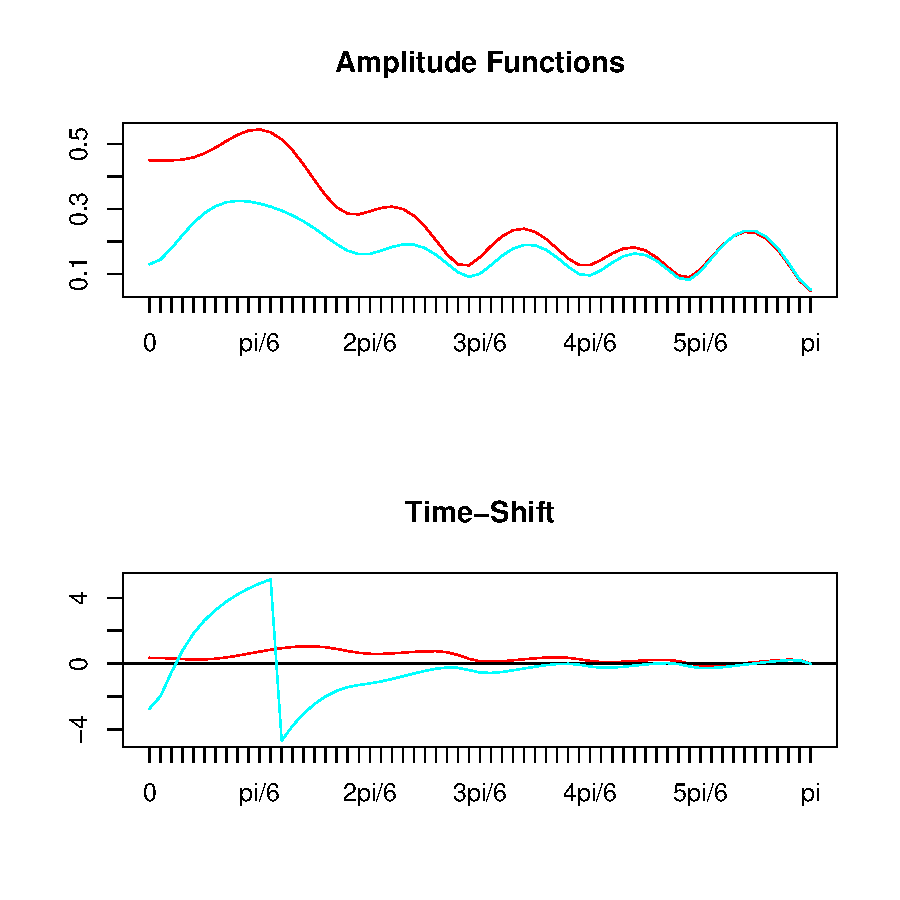
\includegraphics[height=6in, width=6in]{z_mdfa_ar1_amp_shift_Lag_0_iF_i2F.pdf}\caption{Amplitude (top) and time-shift (bottom) functions: unconstrained i1=I2=F\label{z_mdfa_ar1_amp_shift_Lag_0_iF_i2F}}\end{center}\end{figure}No constraints are imposed in frequency zero.
\item Same as above but impose a simple level constraint: $i1=T,i2=F$ and $w^0=\frac{1+\sqrt{5}}{2},w^1=-\sqrt{2}$. Plot and compare the resulting amplitude functions, see fig.\ref{z_mdfa_ar1_amp_shift_Lag_0_iT_i2F}. Hint: we here use the call based on the context-specific function $MDFA_mse_constraint$ whose additional arguments account for the relevant constraints.
\begin{Schunk}
\begin{Sinput}
> # Source the default (MSE-) parameter settings
> source(file=paste(path.pgm,"control_default.r",sep=""))
> # Impose level constraint
> i1<-T
> # Constraints: for series 1 and 2
> weight_constraint<-c((1+sqrt(5))/2,-sqrt(2))
> # Call to the context-specific MDFA_mse_constraint function
> mdfa_obj<-MDFA_mse_constraint(L,weight_func,Lag,Gamma,i1,i2,weight_constraint,
+                               shift_constraint)$mdfa_obj
> file = paste("z_mdfa_ar1_amp_shift_Lag_0_iT_i2F.pdf", sep = "")
> pdf(file = paste(path.out,file,sep=""), paper = "special", width = 6, height = 6)
> K<-nrow(weight_func)-1
> par(mfrow = c(2, 1))
> # amplitude functions
> mplot <- abs(mdfa_obj$trffkt)
> # x-axis
> freq_axe <- rep(NA, K + 1)
> freq_axe[1] <- 0
> freq_axe[1 + (1 : 6) * K / 6] <- c(paste0(c("", 2 : 5), "pi/6"), "pi")
> ax <- freq_axe
> # colors, title and additional titles
> insamp <- 1.e+90
> colo <- NULL
> plot_title <- "Amplitude Functions"
> title_more <- colnames(x[, -1])
> mplot_func(mplot, ax, plot_title, title_more, insamp, colo)
> # time-shift
> mplot <- Arg(t(sign(apply(mdfa_obj$b, 2, sum)) * t(mdfa_obj$trffkt))) /
+       ((0 : (nrow(mdfa_obj$trffkt) - 1)) * pi / (nrow(mdfa_obj$trffkt) - 1))
> # We use the exact formula for the time-shift in frequency zero
> mplot[1, ] <- apply(mdfa_obj$b*(0:(L-1)),2,sum)/apply(mdfa_obj$b, 2, sum)
> plot_title <- "Time-Shift"
> mplot_func(mplot, ax, plot_title, title_more, insamp, colo)
> invisible(dev.off())
> print(c("Level restrictions", round(apply(mdfa_obj$b,2,sum),4)))
\end{Sinput}
\begin{Soutput}
[1] "Level restrictions" "1.618"              "-1.4142"           
\end{Soutput}
\end{Schunk}

\begin{figure}[H]\begin{center}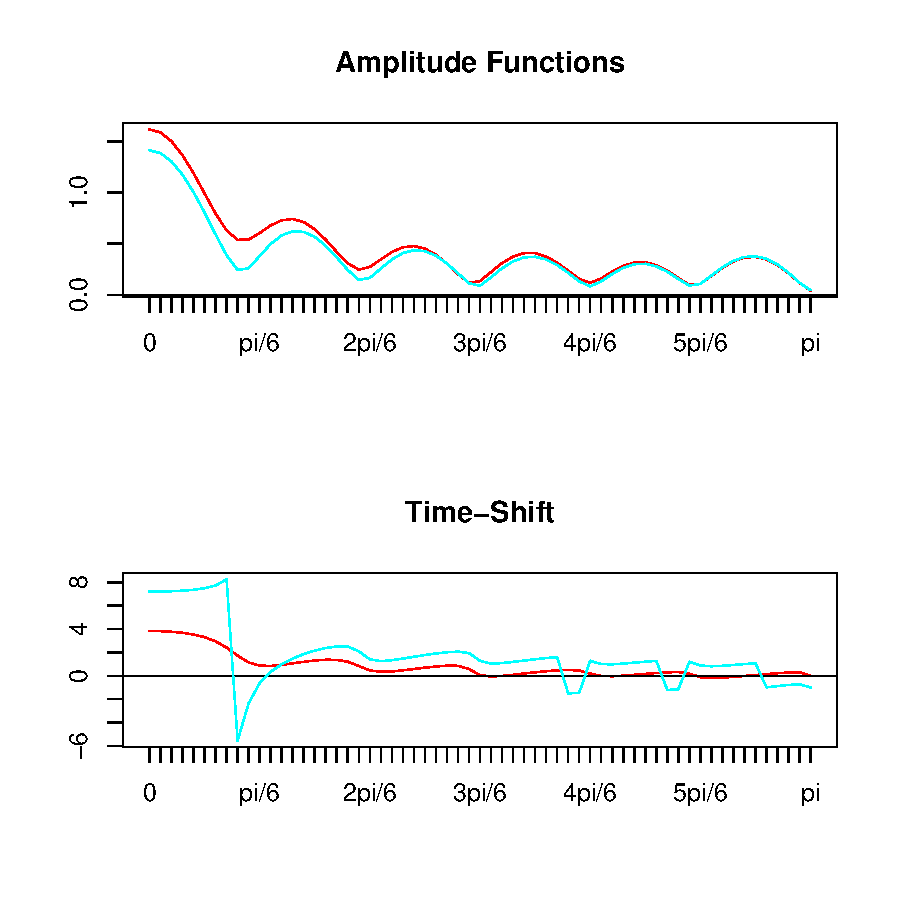
\includegraphics[height=6in, width=6in]{z_mdfa_ar1_amp_shift_Lag_0_iT_i2F.pdf}\caption{Amplitude (top) and time-shift (bottom) functions: i1=T,i2=F\label{z_mdfa_ar1_amp_shift_Lag_0_iT_i2F}}\end{center}\end{figure}As expected, the bivariate transfer function satisfies the imposed first order restrictions $w^0=\frac{1+\sqrt{5}}{2},w^1=-\sqrt{2}$ in frequency zero. Consider that the resulting filter is not obtained by a simple scaling of its coefficients; instead, it is the best (MSE) filter among all those which satisfy the restriction (a simple scaling could not pretend to optimality, in general). 
\item Same as above but impose a simple time-shift restriction, $i1=F,i2=T$, and select $s^0=e=\exp(1),s^1=-\pi$. Compute and compare the time-shift functions, see fig.\ref{z_mdfa_ar1_amp_shift_Lag_0_iF_i2T}.

\begin{Schunk}
\begin{Sinput}
> # Source the default (MSE-) parameter settings
> source(file=paste(path.pgm,"control_default.r",sep=""))#b0_H0
> # Estimate filter coefficients: note that i1<-F by sourcing 
> #   the default parameters
> i2<-T
> shift_constraint<-c(exp(1),-pi)
> mdfa_obj<-MDFA_mse_constraint(L,weight_func,Lag,Gamma,i1,i2,weight_constraint,
+                               shift_constraint)$mdfa_obj
> file = paste("z_mdfa_ar1_amp_shift_Lag_0_iF_i2T.pdf", sep = "")
> pdf(file = paste(path.out,file,sep=""), paper = "special", 
+     width = 6, height = 6)
> K<-nrow(weight_func)-1
> par(mfrow = c(2, 1))
> # amplitude functions
> mplot <- abs(mdfa_obj$trffkt)
> # x-axis
> freq_axe <- rep(NA, K + 1)
> freq_axe[1] <- 0
> freq_axe[1 + (1 : 6) * K / 6] <- c(paste0(c("", 2 : 5), "pi/6"), "pi")
> ax <- freq_axe
> # colors, title and additional titles
> insamp <- 1.e+90
> colo <- NULL
> plot_title <- "Amplitude Functions"
> title_more <- colnames(x[, -1])
> mplot_func(mplot, ax, plot_title, title_more, insamp, colo)
> # time-shift
> mplot <- Arg(t(sign(apply(mdfa_obj$b, 2, sum)) * t(mdfa_obj$trffkt))) /
+       ((0 : (nrow(mdfa_obj$trffkt) - 1)) * pi / (nrow(mdfa_obj$trffkt) - 1))
> # We use the exact formula for the time-shift in frequency zero
> mplot[1, ] <- apply(mdfa_obj$b*(0:(L-1)),2,sum)/apply(mdfa_obj$b, 2, sum)
> plot_title <- "Time-Shift"
> mplot_func(mplot, ax, plot_title, title_more, insamp, colo)
> invisible(dev.off())
> print(c("Time-shift restrictions",
+     round(apply(mdfa_obj$b*(0:(L-1)),2,sum)/apply(mdfa_obj$b, 2, sum),4)))
\end{Sinput}
\begin{Soutput}
[1] "Time-shift restrictions" "2.7183"                  "-3.1416"                
\end{Soutput}
\end{Schunk}

\begin{figure}[H]\begin{center}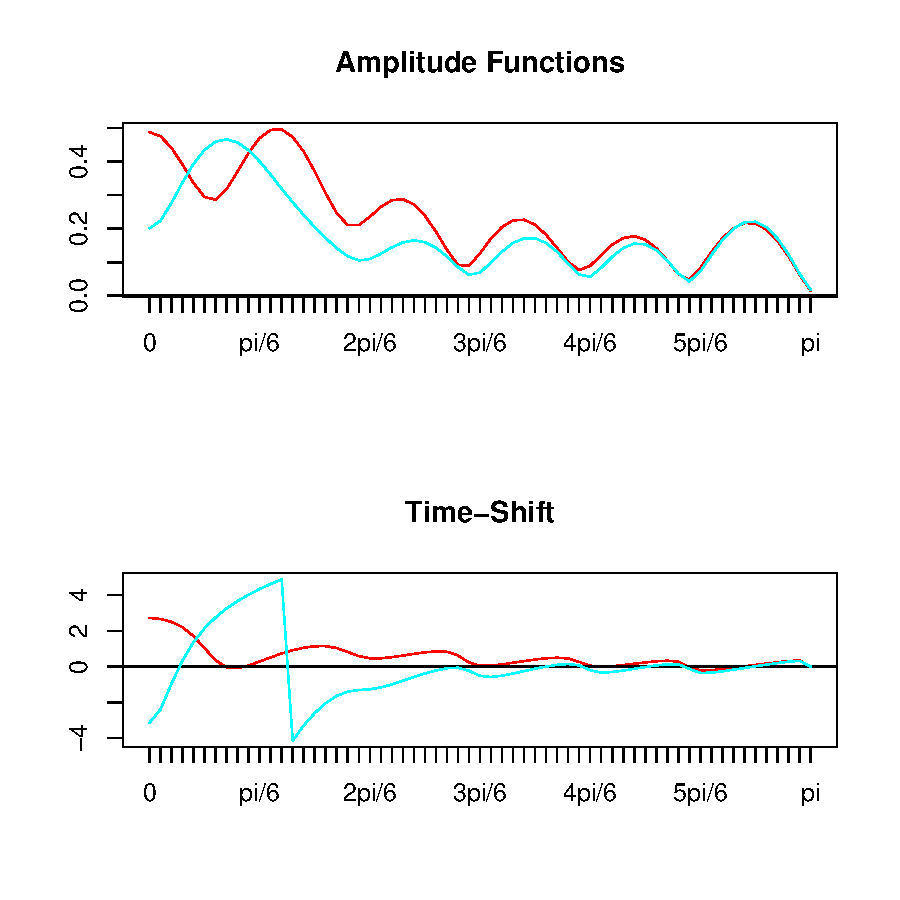
\includegraphics[height=6in, width=6in]{z_mdfa_ar1_amp_shift_Lag_0_iF_i2T.pdf}\caption{Amplitude (top) and time-shift (bottom) functions: i1=F,i2=T\label{z_mdfa_ar1_amp_shift_Lag_0_iF_i2T}}\end{center}\end{figure}The time-shifts agree with our constraints, $s^0=e=\exp(1),s^1=-\pi$, in frequency zero.

\item Impose both constraints simultaneously, see fig.\ref{z_mdfa_ar1_amp_shift_Lag_0_iT_i2T}.

\begin{Schunk}
\begin{Sinput}
> # Source the default (MSE-) parameter settings
> source(file=paste(path.pgm,"control_default.r",sep=""))
> # Impose both constraints
> i1<-T
> i2<-T
> # Specify the constraints
> weight_constraint<-c((1+sqrt(5))/2,-sqrt(2))
> shift_constraint<-c(exp(1),-pi)
> mdfa_obj<-MDFA_mse_constraint(L,weight_func,Lag,Gamma,i1,i2,weight_constraint,
+                               shift_constraint)$mdfa_obj
> file = paste("z_mdfa_ar1_amp_shift_Lag_0_iT_i2T.pdf", sep = "")
> pdf(file = paste(path.out,file,sep=""), paper = "special", 
+     width = 6, height = 6)
> K<-nrow(weight_func)-1
> par(mfrow = c(2, 1))
> # amplitude functions
> mplot <- abs(mdfa_obj$trffkt)
> # x-axis
> freq_axe <- rep(NA, K + 1)
> freq_axe[1] <- 0
> freq_axe[1 + (1 : 6) * K / 6] <- c(paste0(c("", 2 : 5), "pi/6"), "pi")
> ax <- freq_axe
> # colors, title and additional titles
> insamp <- 1.e+90
> colo <- NULL
> plot_title <- "Amplitude Functions"
> title_more <- colnames(x[, -1])
> mplot_func(mplot, ax, plot_title, title_more, insamp, colo)
> # time-shift
> mplot <- Arg(t(sign(apply(mdfa_obj$b, 2, sum)) * t(mdfa_obj$trffkt))) /
+       ((0 : (nrow(mdfa_obj$trffkt) - 1)) * pi / (nrow(mdfa_obj$trffkt) - 1))
> # We use the exact formula for the time-shift in frequency zero
> mplot[1, ] <- apply(mdfa_obj$b*(0:(L-1)),2,sum)/apply(mdfa_obj$b, 2, sum)
> plot_title <- "Time-Shift"
> mplot_func(mplot, ax, plot_title, title_more, insamp, colo)
> invisible(dev.off())
> print(c("Level restrictions", round(apply(mdfa_obj$b,2,sum),4)))
\end{Sinput}
\begin{Soutput}
[1] "Level restrictions" "1.618"              "-1.4142"           
\end{Soutput}
\begin{Sinput}
> print(c("Time-shift restrictions",
+ round(apply(mdfa_obj$b*(Lag:(L-1+Lag)),2,sum)/apply(mdfa_obj$b, 2, sum),4)))
\end{Sinput}
\begin{Soutput}
[1] "Time-shift restrictions" "2.7183"                  "-3.1416"                
\end{Soutput}
\end{Schunk}

\begin{figure}[H]\begin{center}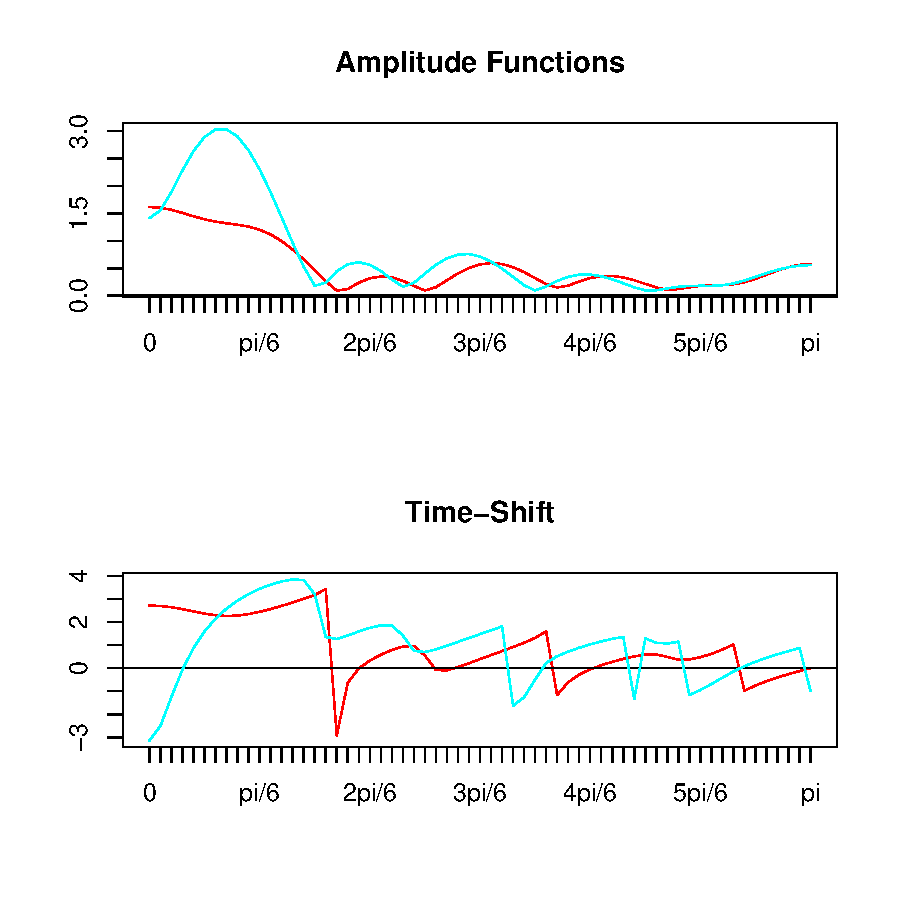
\includegraphics[height=6in, width=6in]{z_mdfa_ar1_amp_shift_Lag_0_iT_i2T.pdf}\caption{Amplitude (top) and time-shift (bottom) functions: i1=i2=T\label{z_mdfa_ar1_amp_shift_Lag_0_iT_i2T}}\end{center}\end{figure}Both functions satisfy the restrictions $w^0=\frac{1+\sqrt{5}}{2},w^1=-\sqrt{2}$ and $s^0=e=\exp(1),s^1=-\pi$, as desired. 

\item To conclude, we briefly analyze the effect of $Lag=-h\neq 0$. Specifically we address a two-step ahead forecast of the target signal and analyze synchronization effects obtained by the time-shift constraint.
\begin{itemize}
\item We rely on the following example: $i1=F$, $i2=T$ (time-shift constraint only\footnote{This setting could not be replicated by classic model-based approaches because the I(2)-shift constraint would assume the I(1)-level constraint as a prerequisite.}), $s^0=1,s^1=2$ and we set $Lag=-2$ (two-step ahead forecast of the signal). This particular example is not selected for its practical relevance; instead we want to illustrate handling of potential singularities  by our code (note that $Lag+s^1=0$).  
\begin{Schunk}
\begin{Sinput}
> # Source the default (MSE-) parameter settings
> source(file=paste(path.pgm,"control_default.r",sep=""))#b0_H0
> # Estimate filter coefficients: note that i1<-F by sourcing the default parameters
> i2<-T
> Lag<--2
> shift_constraint<-c(0,2)
> mdfa_obj<-MDFA_mse_constraint(L,weight_func,Lag,Gamma,i1,i2,weight_constraint,
+                               shift_constraint)$mdfa_obj
> b_mat<-mdfa_obj$b
> trffkt_mdfa<-mdfa_obj$trffkt
> file = paste("z_mdfa_ar1_amp_shift_Lag_0_iF_i2T_Lag.pdf", sep = "")
> pdf(file = paste(path.out,file,sep=""), paper = "special", 
+     width = 6, height = 6)
> K<-nrow(weight_func)-1
> par(mfrow = c(2, 1))
> # amplitude functions
> mplot <- abs(mdfa_obj$trffkt)
> # x-axis
> freq_axe <- rep(NA, K + 1)
> freq_axe[1] <- 0
> freq_axe[1 + (1 : 6) * K / 6] <- c(paste0(c("", 2 : 5), "pi/6"), "pi")
> ax <- freq_axe
> # colors, title and additional titles
> insamp <- 1.e+90
> colo <- NULL
> plot_title <- "Amplitude Functions"
> title_more <- colnames(x[, -1])
> mplot_func(mplot, ax, plot_title, title_more, insamp, colo)
> # time-shift
> mplot <- Arg(t(sign(apply(mdfa_obj$b, 2, sum)) * t(mdfa_obj$trffkt))) /
+       ((0 : (nrow(mdfa_obj$trffkt) - 1)) * pi / (nrow(mdfa_obj$trffkt) - 1))
> # We use the exact formula for the time-shift in frequency zero
> mplot[1, ] <- apply(mdfa_obj$b*(0:(L-1)),2,sum)/apply(mdfa_obj$b, 2, sum)
> plot_title <- "Time-Shift"
> mplot_func(mplot, ax, plot_title, title_more, insamp, colo)
> invisible(dev.off())
> print(c("Time-shift restrictions",
+         round(apply(mdfa_obj$b*(0:(L-1)),2,sum)/
+           apply(mdfa_obj$b, 2, sum),4)))
\end{Sinput}
\begin{Soutput}
[1] "Time-shift restrictions" "-2"                      "0.01"                   
\end{Soutput}
\end{Schunk}

\begin{figure}[H]\begin{center}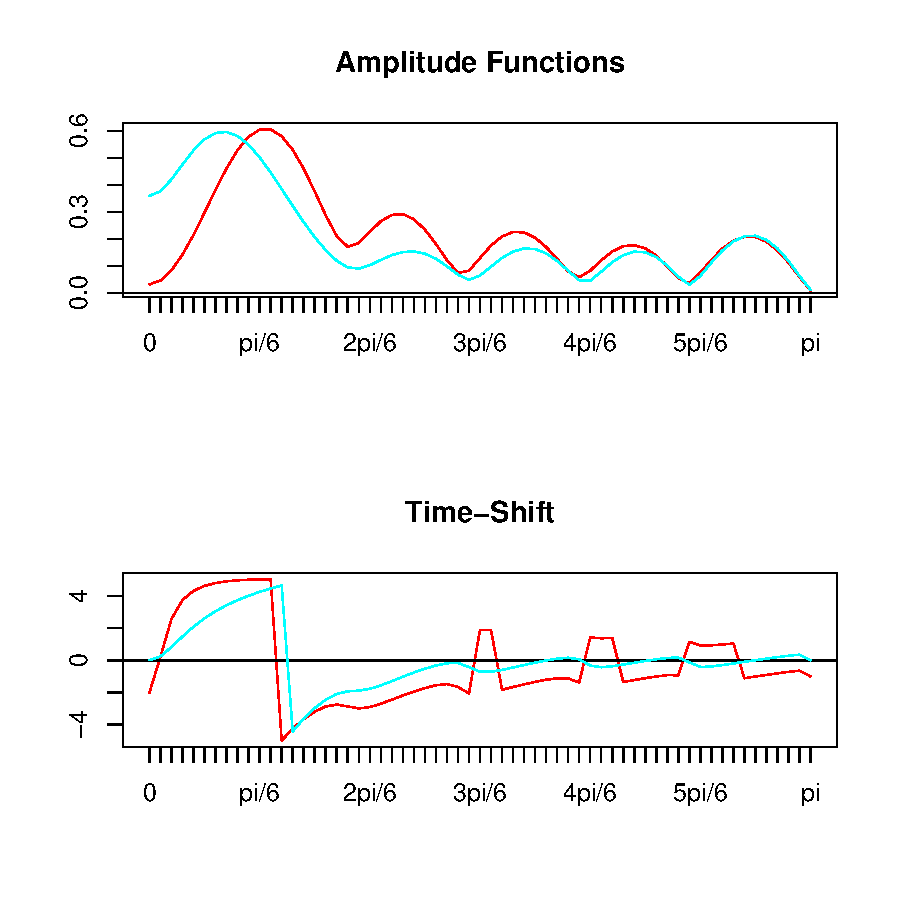
\includegraphics[height=6in, width=6in]{z_mdfa_ar1_amp_shift_Lag_0_iF_i2T_Lag.pdf}\caption{Amplitude (top) and time-shift (bottom) functions: i1=F,i2=T, Lag=-2\label{z_mdfa_ar1_amp_shift_Lag_0_iF_i2T_Lag}}\end{center}\end{figure}The first time-shift agrees with our constraints when shifted by $Lag$: $s^0+Lag=0-2=-2$. The second time-shift should be $s^1+Lag=2-2=0$ which would generate a singularity (dividing by zero); in order to circumvent the problem we `shift the shift' by a small constant (0.01) in our code: the resulting effect should be negligible by all practical means and the trick allows a much simpler implementation of the constraints in the considered case (i1=F,i2=T). 
\item Feed a signal to the filters of the the bivariate design and verify the time-shift constraints. Hints: we generate two filter outputs, one for each filter; since the constraints apply in frequency zero, our input signals are   linear trends (signals of frequency zero); since our amplitude functions are not normalized to one, in frequency zero, we need to normalize the output signals (by the inverse of the transfer functions in frequency zero).
\begin{Schunk}
\begin{Sinput}
> len_t<-100
> # Generate two linear trends (they are shifted by a constant 
> # in order to be distinguished)
> trend_data<-cbind(1:len_t,0.5+1:len_t)
> # Compute both output series: normalize by the inverse 
> #   transferfunctions in frequency zero
> yhat_multivariate<-cbind(rep(NA,len_t),rep(NA,len_t))
> for (i in 1:ncol(yhat_multivariate))
+   for (j in L:len_t)
+ #  The transfer function in frequency zero is a real number: 
+ #   R computes a complex number with vanishing imaginary part. 
+ #   We have to extract the real part because otherwise the complex 
+ #   series would not be plotted... 
+     yhat_multivariate[j,i]<-sum(b_mat[,i]*trend_data[j:(j-L+1),i])/
+       Re(trffkt_mdfa[1,i])
> mplot<-cbind(trend_data,yhat_multivariate)
> dimnames(mplot)[[2]]<-c("Input 1","Input 2","Output 1","Output 2")
> # Display the last observations
> tail(mplot)
\end{Sinput}
\begin{Soutput}
       Input 1 Input 2 Output 1 Output 2
 [95,]      95    95.5       97    95.49
 [96,]      96    96.5       98    96.49
 [97,]      97    97.5       99    97.49
 [98,]      98    98.5      100    98.49
 [99,]      99    99.5      101    99.49
[100,]     100   100.5      102   100.49
\end{Soutput}
\end{Schunk}
We observe that `Output 1' leads `Input 1' by two time units, as desired. `Output 2' is almost synchronized with `Input 2'  up to the small correction by 0.01 (to avoid singular expressions in the R-code). 

\end{itemize}

\end{enumerate}
The chosen real-numbered constraints in the above exercises illustrate that arbitrary (real or integer-numbered) restrictions can be imposed. Whether they are useful, or not, depends on the particular application (integration order of the DGP) as well as on the particular research priorities of the user (MSE or turning points). 


\section{Summary}


\begin{itemize}
\item We proposed a set of  filter restrictions which affect the level and the time-shift of the filter outputs. 
\item We extended the stationary DFA-criterion to non-stationary integrated processes. A generalization to multivariate filters is proposed in chapter \ref{coint_sec}.
\item Given a non-stationary I(1)- or I(2)-input signal $x_t$ and a generic target specification $\Gamma(\omega)$, the output $\hat{y}_t$ of the constrained forecast-, nowcast- or backcast-filter $\hat{\Gamma}(\omega)$ is able to track the signal in the sense that the filter error remains stationary (cointegration). \item In practice, one is often interested in a vanishing time-shift whether the data is integrated or not.
\item The proposed restrictions apply independently to each time series of a multivariate design. Cross-sectional links (cointegration) are proposed and discussed in chapter \ref{coint_sec}.
\item We proposed a formal matrix implementation and derived a generalized optimization criterion. The unconstrained case, proposed in the previous chapters, is nested in the proposed solution.
\end{itemize}

%----------------------------------------








\chapter{ATS-Trilemma: the Univariate Case}\label{ats_sec}

We propose an extension of the classic MSE-paradigm which addresses nowcast and forecast applications\footnote{Backcasts were discussed in chapter \ref{fil_sec}.}. Specifically, we split the original MSE-norm into three components, identified as Accuracy, Timeliness and Smoothness. The resulting two-dimensional trade-off, controlled by the parameter-pair $\lambda,\eta$ in the head of the main function call, is called Accuracy-Timeliness-Smoothness Trilemma, or ATS-Trilemma for short, see Wildi (2005), McElroy and Wildi (2015). We derive  a generic optimization principle, called Customization, which nests the classic MSE-approach.  We show that the ATS-trilemma collapses to a one-dimensional trade off, the so-called AT-dilemma, in the case of forecasting. We infer  that classic (pseudo-maximum likelihood)  one-step ahead forecast approaches are incapable of addressing Timeliness and Smoothness, simultaneously. Efficiency gains of customized designs are quantified in a series of empirical examples. \\

The ATS-trilemma and the generic customization principle are introduced in section \ref{seatatst}; section \ref{fatatd} highlights the classic dichotomic forecast paradigm; quadratic optimization criteria and closed-form solutions are presented in section \ref{idfas}; an application of customization is proposed in section \ref{ats_work_o}; performance measures are presented in section \ref{peco_cu}; finally, sections \ref{double_score_ats} and \ref{ucdvbmseli} assess performances of customized designs when benchmarked against classic MSE-approaches. 











\section{Signal Extraction and the ATS-Trilemma}\label{seatatst}

We address the univariate dfa-case and generalize criterion \ref{dfa_ms}. Our treatment follows \href{http://blog.zhaw.ch/sef/files/2014/10/DFA.pdf}{DFA}, section 4.3, and McElroy and Wildi (2015). 


\subsection{Decomposition of the MSE-Norm}

The DFA emphasizes the so-called transferfunction-error $\Gamma(\cdot)-\hat{\Gamma}(\cdot)$. The following geometric identity holds in general (law of cosine in the complex plane):
\begin{eqnarray}
|\Gamma(\omega)-\hat{\Gamma}(\omega)|^2&=&A(\omega)^2+\hat{A}(\omega)^2-2A(\omega)
\hat{A}(\omega)\cos\left(\hat{\Phi}(\omega)-\Phi(\omega)\right)\nonumber\\
&=&
(A(\omega)-\hat{A}(\omega))^2\nonumber\\
&&+2A(\omega)\hat{A}(\omega)\left[1-\cos\left(\hat{\Phi}(\omega)-\Phi(\omega)\right)\right]\label{etrigid}
\end{eqnarray}
If $\Gamma$ is symmetric and positive, then \(\Phi(\omega)\equiv
0\) so that we can omit $\Phi(\omega)$ from our notation\footnote{The ideal trend, classical filters (HP, CF, henderson) or model-based filters are typically positive (symmetric) filters. It should be clear that $\Phi(\omega)$ cannot be omitted if the condition is unfulfilled.}. By inserting \ref{etrigid} into \ref{dfa_ms} and using
$1-\cos(\hat{\Phi}(\omega))=2\sin(\hat{\Phi}(\omega)/2)^2$ we obtain
\begin{eqnarray} &&\frac{2\pi}{T}\sum_{k=-[T/2]}^{[T/2]}\left|\Gamma(\omega_k)-\hat{\Gamma}(\omega_k) \right|^2 I_{TX}(\omega_k)\nonumber\\
&=&\frac{2\pi}{ T} \sum_{k=-T/2}^{T/2}
(A(\omega_k)-\hat{A}(\omega_k))^2 I_{TX}(\omega_k)\label{unboptidioe}\\
&&+\frac{2\pi}{ T} \sum_{k=-T/2}^{T/2}
4A(\omega_k)\hat{A}(\omega_k)\sin(\hat{\Phi}(\omega_k)/2)^2
I_{TX}(\omega_k)\label{unboptidio}
\end{eqnarray}
The first summand \ref{unboptidioe} is the distinctive part of the total mean-square filter error
which is attributable to the amplitude function of the real-time filter (the MS-amplitude error).
The second summand \ref{unboptidio} measures the distinctive contribution of the phase or time-shift to
the total mean-square error (the MS-time-shift error). Note that the product
$A(\omega_k)\hat{A}(\omega_k)I_{TX}(\omega_k)$ in \ref{unboptidio} maps the scales of the filter outputs $y_t,\hat{y}_t$ to the frequency-domain (the phase function alone would be dimensionless).



\subsection{Accuracy, Timeliness and Smoothness (ATS-) Error-Components}  \label{ats_section}



The previous decomposition can be refined by splitting
each term into contributions from \emph{pass-} and \emph{stopbands}. For ease of exposition we assume an ideal lowpass target 
\[\Gamma(\omega)=\left\{\begin{array}{cc}1~,~|\omega|\leq\textrm{cutoff}\\0~,~\textrm{otherwise}\end{array}\right.\]
The set $\{\omega_k||\omega_k|\leq\textrm{cutoff}\}$ corresponds to the passband and its complement $\{\omega_k||\omega_k|>\textrm{cutoff}\}$ is the stop- or rejection-band. We now define
\begin{eqnarray}
\left.\begin{array}{ccc}
\textrm{A(ccuracy)}&:=&\frac{2\pi}{ T} \sum_{\textrm{Passband}} (A(\omega_k)-\hat{A}(\omega_k))^2 I_{TX}(\omega_k)\\
\textrm{S(moothness)}&:=&\frac{2\pi}{ T} \sum_{\textrm{Stopband}} (A(\omega_k)-\hat{A}(\omega_k))^2 I_{TX}(\omega_k)\\
\textrm{T(imeliness)}&:=&\frac{2\pi}{ T}  \sum_{\textrm{Passband}} 4A(\omega_k)\hat{A}(\omega_k)\sin(\hat{\Phi}(\omega_k)/2)^2
I_{TX}(\omega_k)                                     \\
\textrm{R(esidual)}&:=&\frac{2\pi}{ T}  \sum_{\textrm{Stopband}} 4A(\omega_k)\hat{A}(\omega_k)\sin(\hat{\Phi}(\omega_k)/2)^2
I_{TX}(\omega_k)
\end{array}\right\}\label{mse_dec_ats}
\end{eqnarray}
\begin{itemize}
\item \emph{Residual} is that part of the MSE which is contributed by the time-shift in the stopband: it \emph{vanishes} exactly in the case of the ideal trend.  Even if it does not vanish, it is generally negligible because the product $A(\omega_k)\hat{A}(\omega_k)$ is small in the stopband. We now ignore this error-term (it is dropped from subsequent notation).
\item \emph{Accuracy} measures the contribution to the MSE-norm which would be obtained by ignoring time-shift (passband) and noise suppression (stop-band) issues\footnote{It is the performance of a symmetric filter (no time-shift) with perfect noise suppression ($\hat{A}(\cdot)=\Gamma(0)=0$ in
the stopband) and with the same amplitude as $\hat{\Gamma}(\cdot)$ in the passband. Such a design could be easily constructed by
the techniques presented in \href{http://blog.zhaw.ch/sef/files/2014/10/DFA.pdf}{DFA}, section 1.}.
\item \emph{Smoothness} measures the contribution to total MSE of the undesirable high-frequency noise, leaking
from the imperfect amplitude fit in the stopband (convolution theorem \ref{convolution_dft}). This measure is tightly linked to classical time-domain \emph{curvature} (smoothness) measures.
\item \emph{Timeliness} measures the MSE-contribution generated by the time-shift. This measure is closely linked
to the well-known (time-domain) \emph{peak-correlation}, as referenced against the target signal.
\end{itemize}
We are now able to address each single or each \emph{pairwise} combination of error-terms by splitting the MSE-criterion accordingly. Typically, speed (Timeliness) and noise suppression (Smoothness) are important properties of a real-time filter in prospective estimation problems (nowcast, forecast)  



\subsection{Generic Customized Criterion}\label{gen_cust_crit}


We are in a position to generalize the mean-square optimization criterion \ref{dfa_ms}
by assigning weights to the ATS-components (recall that the Residual either vanishes exactly or is negligible):
\begin{equation}\label{ats_cust}
\textrm{MSE-Cust}(\lambda_1,\lambda_2)=\textrm{Accuracy}+(1+\lambda_1) \textrm{Timeliness}+(1+\lambda_2) \textrm{Smoothness}\to \min_{\mathbf{b}}
\end{equation}
Selecting $\lambda_1>0$ results, ceteris paribus, in a smaller Timeliness component; as we shall see the resulting filter will be faster: turning-points can be detected earlier (smaller peak-correlation against the target signal). Selecting
$\lambda_2>0$ magnifies, ceteris paribus, the Smoothness term: the output of the resulting filter is smoother or, stated otherwise, undesirable high-frequency noise is damped more effectively. Finally, selecting $\lambda_1>0,\lambda_2>0$ emphasizes both attributes: the resulting filter-output is able to gain both in terms of `speed' as well as in terms of `noise suppression'. The ATS-trilemma confers the user the possibility to adjust trade-offs according to research priorities.\\


The schematic criterion \ref{ats_cust} can be generalized by substituting weighting functions $W_1(\omega_k)\geq 0$, $W_2(\omega_k)\geq 0$  for the fixed weights $\lambda_1,\lambda_2$:
\begin{eqnarray*}
&&\frac{2\pi}{ T} \sum_{\textrm{Passband}} (A(\omega_k)-\hat{A}(\omega_k))^2 I_{TX}(\omega_k)\nonumber\\
&&+\frac{2\pi}{ T} \sum_{\textrm{Stopband}} (A(\omega_k)-\hat{A}(\omega_k))^2 W_2(\omega_k)I_{TX}(\omega_k)\nonumber\\
&&+\frac{2\pi}{ T}  \sum_{\textrm{Passband}} 4A(\omega_k)\hat{A}(\omega_k)\sin(\hat{\Phi}(\omega_k)/2)^2
W_1(\omega_k)I_{TX}(\omega_k)\to\min_{\mathbf{b}}
\end{eqnarray*}
Criterion \ref{ats_cust} can be replicated by selecting
\begin{eqnarray*}
W_1(\omega_k,\lambda_1)&=&1+\lambda_1\\
W_2(\omega_k,\lambda_2)&=&1+\lambda_2
\end{eqnarray*}
Note, however, that $W_2$ would introduce an undesirable discontinuity in the cutoff-frequency, if $\lambda_2\neq 0$. Therefore, we propose the following weighting-scheme
\begin{eqnarray}
\left.\begin{array}{ccc}W_1(\omega_k,\lambda)&=&1+\lambda\\
W_2(\omega_k,\eta)&=&(1+|\omega_k|-\textrm{cutoff})^{\eta}
\end{array}\right\}\label{w_func_cust}
\end{eqnarray}
The new function $W_2$ allows for a continuous transition from pass- to stopband and its monotonic shape overemphasizes undesirable high-frequency components\footnote{The `nuisance' of an undesirable high-frequency component, as measured by its derivative (or its first-order difference) is proportional to $\omega$ (or to $|1-\exp(-i\omega)|$).}. We re-labelled
$\lambda_1,\lambda_2$ by $\lambda,\eta$ in order to distinguish symbolically both effects: $\lambda>0$ emphasizes Timeliness and $\eta>0$ addresses Smoothness. The criterion can be re-written more compactly as
\begin{eqnarray}
&&\frac{2\pi}{ T} \sum_{\textrm{All~Frequencies}} (A(\omega_k)-\hat{A}(\omega_k))^2 W(\omega_k,\eta) I_{TX}(\omega_k)\nonumber\\
&&+(1+\lambda)\frac{2\pi}{ T}  \sum_{\textrm{Passband}} 4A(\omega_k)\hat{A}(\omega_k)\sin(\hat{\Phi}(\omega_k)/2)^2
I_{TX}(\omega_k)\to\min_{\mathbf{b}}\label{dfatp}
\end{eqnarray}
where
\begin{equation}\label{w}
W(\omega_k,\eta,\textrm{cutoff})=\left\{\begin{array}{cc}
1~,~\textrm{if~} |\omega_k|<\textrm{cutoff}\\
(1+|\omega_k|-\textrm{cutoff})^{\eta}~,~\textrm{otherwise}
\end{array}\right.
\end{equation}
The optimization principle \ref{dfatp} is called a \emph{customized} criterion, see Wildi (2005) and McElroy and Wildi (2015). Obviously, the customized criterion nests the MSE-criterion \ref{dfa_ms} (select $\lambda=\eta=0$).  


\section{Forecasting and the AT-Dilemma}\label{fatatd}

In the previous section we assumed a particular signal as specified by a lowpass target. Here we analyze (anticipative) \emph{allpass} targets which appear in classical forecast applications, recall section \ref{one_step}.    

\subsection{ATS-Trilemma Collapses to AT-Dilemma}

An application of the MDFA-MSE criterion \ref{dfanv} to ordinary one- (and multi-) step head forecasting was proposed in section \ref{one_step}. Specifically, in the case of the classic one-step ahead criterion, \ref{dfa_ms} becomes 
\begin{equation}\label{dfanv_1s_ats}
\frac{2\pi}{T} \sum_{k=-T/2}^{T/2}
\left|\exp(i\omega_k)-\hat{\Gamma}_X(\omega_k)\right|^2I_{T
X}(\omega_k) \to \min_{\mathbf{b}}
\end{equation}
Note that the target filter $\Gamma(\omega_k):=\exp(i\omega_k)$ is an allpass since $|\Gamma(\omega_k)|=1$ for all frequencies. As a consequence, both the Residual- as well as the Smoothness-term vanish -- they are missing -- and (the schematic) criterion  \ref{ats_cust} simplifies to
\begin{eqnarray*}
\textrm{MSE-Cust}(\lambda_1)=\textrm{Accuracy}+(1+\lambda_1) \textrm{Timeliness}\to \min_{\mathbf{b}}
\end{eqnarray*}
The signal-extraction ATS-trilemma collapses to a forecast {AT-dilemma}. We may infer that the classic time series paradigm (pseudo-maximum-likelihood), which relies on (mean-square one-step ahead) forecast performances is immanently unable to break-up the tie between Timeliness and Smoothness in real-time signal extraction.  




\subsection{Illustration: White Noise and Random-Walk Processes}\label{i_w_rw}

\subsubsection{LDP-Filter and Arithmetic Mean}

Let $\Gamma(\omega_k)=\exp(i\omega_k)$ be the one-step ahead target and consider the following two polar filter designs: 
\begin{enumerate}
\item Let $b_0=1,b_j=0,j=1,...,L-1$: the filter assigns full weight $b_0=1$ to $x_T$ in the data-sample $x_1,...,x_T$. Let's call it `Last-Data-Point' (LDP-) filter. Its transfer function is
\[\hat{\Gamma}(\omega_k)=1\]
\item Let $b_j=1/L,j=0,...,L-1$: the filter assigns equal weight $1/L$ to $x_T,...,x_{T-(L-1)}$. We now set $L:=T$ so that the equal-weight filter corresponds to the arithmetic mean. The transfer function of the arithmetic mean is
\[\hat{\Gamma}(\omega_k)=\frac{1}{T}\sum_{j=0}^{T-1}\exp(-ij\omega_k)\]
\end{enumerate}
The LDP-filter is an allpass without time-shift; the arithmetic mean is a lowpass with a narrow passband and a large time-shift. 



\subsubsection{Random-Walk Process}

Let $x_1,...,x_T$ be a realization of a random-walk process. In this case, the LDP-filter is optimal, in a mean-square one-step ahead perspective: the best forecast of $x_{T+1}$ is $x_T$. Since Smoothness is missing (no stop-band), the (schematic) customized criterion \ref{ats_cust} simplifies -- degenerates -- to
\begin{eqnarray}
\textrm{MSE-Cust}(\lambda_1)&=&\textrm{Accuracy}+(1+\lambda_1) \textrm{Timeliness}~\left(\to\min_{\mathbf{b}}\right)\label{mdfa_cust_forec}\\
&=&\frac{2\pi}{ T} \sum_{\textrm{All ~Frequencies}} (A(\omega_k)-\hat{A}(\omega_k))^2 I_{TX}(\omega_k)\nonumber\\
&&+(1+\lambda_1)\frac{2\pi}{ T}  \sum_{\textrm{All~Frequencies}} 4A(\omega_k)\hat{A}(\omega_k)\sin\left(\frac{\Phi(\omega_k)-\hat{\Phi}(\omega_k)}{2}\right)^2I_{TX}(\omega_k)\nonumber\\
&=&(1+\lambda_1)\frac{2\pi}{ T}  \sum_{\textrm{All~Frequencies}} 4\sin\left(\omega_k/2\right)^2I_{TX}(\omega_k)~\left(\to\min_{\mathbf{b}}\right)\label{ast_cust_for}
\end{eqnarray}
The last equality follows from $A(\omega_k)=\hat{A}(\omega_k)=1$ (both the target as well as the LDP-filter are allpass designs), $\Phi(\omega_k)=\textrm{Arg}(\exp(i\omega_k))=\omega_k$ (the target filter is anticipative) and $\hat{\Phi}(\omega_k)=0$. We infer that MSE is entirely attributable to Timeliness (Accuracy vanishes); indeed, the output $x_T$ of $\hat{\Gamma}(\cdot)$ is shifted by one time-unit relative to the target $x_{T+1}$: no other action or effect is supported by the LDP-filter. In contrast, the arithmetic mean would strongly smooth the filter output: Accuracy would inflate considerably in \ref{mdfa_cust_forec}.\\

The (true) pseudo-spectrum of the process is given by 
\begin{eqnarray}\label{pseudo_spectrum}
h_X(\omega)=\frac{\sigma^2}{2\pi|1-\exp(-i\omega)|^2}
\end{eqnarray} 
where $\sigma^2$ is the variance of the (stationary) white noise $\tilde{x}_t=x_t-x_{t-1}$ and $\displaystyle{\frac{\sigma^2}{2\pi}}$ is its (flat) spectral-density;  $\displaystyle{\frac{1}{1-\exp(-i\omega)}}$ is the transfer function of the (non-stationary) AR(1)-filter linking the noise $\tilde{x}_t$ to the random-walk $x_t$, see also section \ref{pseudo_dft}. We could now plug the true pseudo-spectrum into \ref{ast_cust_for} and set $\lambda_1=0$ to obtain a so-called `true' MSE%\footnote{The rationale for this substitution is given by \ref{add_res_dfa} i.e. one would minimize the true (unknown) mean-square filter error.} 
\begin{eqnarray}
\textrm{true~MSE}&=&\frac{2\pi}{ T}  \sum_{\textrm{All~Frequencies}} 4\sin\left(\omega_k/2\right)^2\frac{\sigma^2}{2\pi|1-\exp(-i\omega_k)|^2}\nonumber\\
&=&\frac{2\sigma^2}{ T}  \sum_{\textrm{All~Frequencies}} \frac{1-\cos(\Phi(\omega_k))}{|1-\exp(-i\omega_k)|^2}\nonumber\\
&=&\frac{2\sigma^2}{ T}  \sum_{\textrm{All~Frequencies}} \frac{1}{2}\label{rwmse}\\
&=&\sigma^2\nonumber
\end{eqnarray}
where we used $|1-\exp(-i\omega_k)|^2=(1-\cos(\omega_k))^2+\sin(\omega_k)^2=2-2\cos(\omega_k)$\footnote{For notational simplicity we did not discriminate the case of odd and even $T$: in the latter case additional weights $w_k$ would be necessary, see section \ref{dft_and_per}.}. The `true MSE' is the mean-square one-step ahead forecast error, as expected.



\subsubsection{White Noise}


Assume $x_t$ is a white noise process and consider, once again, the LDP-filter. From the above we have 
\begin{eqnarray}
\textrm{MSE-Cust}(\lambda_1)&=&(1+\lambda_1)\frac{2\pi}{ T}  \sum_{\textrm{All~Frequencies}} 4\sin\left(\omega_k/2\right)^2I_{TX}(\omega_k)~\left(\to\min_{\mathbf{b}}\right)\label{ast_cust_for_wn}
\end{eqnarray}
Setting $\lambda_1=0$ and plugging the (flat) spectral density $\displaystyle{\frac{\sigma^2}{2\pi}}$ of the process into this expression %\footnote{The rationale for this substitution is given by \ref{add_res_dfa} i.e. one would minimize the true (unknown) mean-square filter error.} 
we obtain 
\begin{eqnarray}
\textrm{true~MSE}&=&\frac{2\pi}{ T}  \sum_{\textrm{All~Frequencies}} 4\sin(\omega_k/2)^2\frac{\sigma^2}{2\pi}\nonumber\\
&=&\frac{\sigma^2}{ T}  \sum_{\textrm{All~Frequencies}} 4\sin(\omega_k/2)^2\nonumber\\
&=&\frac{2\sigma^2}{ T}  \sum_{\textrm{All~Frequencies}} (1-\cos(\omega_k))\label{wnmse}\\
&=&2\sigma^2\nonumber
\end{eqnarray}
where we made use of $\sum_{\textrm{All~Frequencies}} \cos(\omega_k)=0$, see corollary \ref{discret_sums_cor} in the \ref{dstt}. Indeed, the (true) MSE of the LDP-filter is $Var(x_{T+1}-x_{T})=2\sigma^2$. Comparing \ref{wnmse} and \ref{rwmse} reveals that high-frequency components contribute disproportionate to Timeliness since $1-\cos(\omega_k)$ is monotonically increasing. We now substitute the arithmetic mean for the LDP-filter and obtain:
\begin{eqnarray}
\textrm{true~MSE}&=&\textrm{Accuracy+Timeliness}\nonumber\\
&=&\frac{2\pi}{ T} \sum_{\textrm{All ~Frequencies}} (A(\omega_k)-\hat{A}(\omega_k))^2 \frac{\sigma^2}{2\pi}\nonumber\\
&&+\frac{2\pi}{ T}  \sum_{\textrm{All~Frequencies}} 4A(\omega_k)\hat{A}(\omega_k)\sin\left(\frac{\Phi(\omega_k)-\hat{\Phi}(\omega_k)}{2}\right)^2\frac{\sigma^2}{2\pi}\nonumber\\
&=&\frac{2\pi}{ T} \sum_{\textrm{All ~Frequencies}} \left(1-\left|\frac{1}{T}\sum_{j=0}^{T-1}\exp(-ij\omega_k)\right|\right)^2\frac{\sigma^2}{2\pi} \nonumber\\
&&+\frac{2\pi}{ T}  \sum_{\textrm{All~Frequencies}} 4\left|\frac{1}{T}\sum_{j=0}^{T-1}\exp(-ij\omega_k)\right| \sin\left(\frac{-\omega_k-\frac{T}{2}\omega_k}{2}\right)^2\frac{\sigma^2}{2\pi}\nonumber
\end{eqnarray}
where we inserted $\Phi(\omega_k)=-Arg(\exp(i\omega_k))=-\omega_k$ (anticipative allpass target) and $\hat{\Phi}(\omega_k)=\hat{\phi}(\omega_k)\omega_k=\displaystyle{\frac{T}{2}}\omega_k$\footnote{The equally-weighted (arithmetic mean) filter shifts all components by half its filter-length $L/2$ and we selected $L=T$. Therefore $\hat{\phi}(\omega_k)=T/2$.}. 
Using $\frac{1}{T}\sum_{j=0}^{T-1}\exp(-ij\omega_k)=0, \omega_k\not= 0$, see proposition \ref{discret_sums} in the appendix \ref{dstt}, and the fact that the sine function vanishes at $\omega_0=0$, the expression for the (true) MSE simplifies to
\begin{eqnarray}
\textrm{MSE}&=&\frac{2\pi}{ T} \sum_{\textrm{All ~Frequencies}} \left(1-\left|\frac{1}{T}\sum_{j=0}^{T-1}\exp(-ij\omega_k)\right|\right)^2\frac{\sigma^2}{2\pi} \nonumber\\
&=&\sigma^2\frac{T-1}{T}\label{mse_ins}
\end{eqnarray}
Timeliness vanishes completely because $\hat{A}(\omega_k)=\left|\frac{1}{T}\sum_{j=0}^{T-1}\exp(-ij\omega_k)\right|=0$ if $\omega_k\neq 0$ and because $\sin\left(\frac{\omega_0-\frac{T}{2}\omega_0}{2}\right)=0$ for $\omega_0=0$. Also, the summand of the Accuracy term vanishes in $\omega_0$; therefore Accuracy sums to $\displaystyle{\frac{T-1}{T}}\sigma^2$. The asymptotically negligible correction $\displaystyle{\frac{T-1}{T}}$ accounts for the fact that the arithmetic mean is an in-sample estimate i.e. we observe a tiny bit of overfitting here (the fit in frequency zero is `too good'). We conclude that the (optimal) arithmetic mean trades the entire Timeliness term against a full-blown Accuracy term\footnote{Figuratively, the arithmetic mean squeezes the data to a flat line which is free of time-shifts.}. The net result is that MSE decreases from $2\sigma^2$, in the case of the LDP filter, to $\approx\sigma^2$ (ignoring the finite sample correction).\\

The fact that the arithmetic mean, a strong smoothing filter with a large time-shift, reduces Timeliness is not without a touch of irony\footnote{This is because Timeliness is not a scale-invariant measure i.e. the contribution of the time-shift to MSE depends on the magnitude of the signals. See section \ref{peco_cu} for a corresponding scale-invariant metric.}; even more so when considering that the decrease in Timeliness must overcompensate the inflated Accuracy; and exceedingly so when considering that Smoothness does not even appear in criterion \ref{mdfa_cust_forec} since the forecast-target is an \emph{allpass}. Hopefully, the proposed counter-intuitive examples shed some light on the rich(er) structure of the ATS-trilemma or, for that matter, of its degenerate sibling, the forecast AT-dilemma. 



\section{Quadratic Criterion$^*$}\label{idfas}

\subsection{I-DFA}


The mean-square error criterion \ref{dfa_ms} is a quadratic function of the filter coefficients $\mathbf{b}$ and can be solved  in closed-form, see \ref{bregms}: the solution is unique and numerical computations are fast. Unfortunately, \ref{dfatp} is no longer quadratic in $\mathbf{b}$, if $\lambda>0$. We here propose an alternative expression which is quadratic irrespective of $\lambda$. Interestingly, the new quadratic criterion matches closely \ref{dfatp}, even for `large' $\lambda$ (virtuous feedback loop\footnote{Larger $\lambda$ tend to linearize the problem because $\hat{\Phi}(\omega)-\Phi(\omega)$ will be small, see section \ref{ti_o_app_idfa}.}). Our treatment is general i.e. the target $\Gamma(\cdot)$ does not need to be positive and real. Moreover, the proposed formalism lends itself for a straightforward generalization to the multivariate case, to be developed in chapter \ref{atsm_sec}. Consider
\begin{eqnarray}\label{idfa}
&&\frac{2\pi}{T} \sum_{k=-[T/2]}^{[T/2]}
 \left|\big|\Gamma(\omega_k)\Xi_{TX}(\omega_k)\big|-\left\{\Re\left[\hat{\Gamma}(\omega_k)\Xi_{TX}(\omega_k)\exp\big(-i\arg\big\{\Gamma(\omega_k)\Xi_{TX}(\omega_k)\big\}\big)\right]\right.\right.\nonumber\\
 &&\left.\left.+i\sqrt{1+\lambda|\Gamma(\omega_k)|}
 \Im\left[\hat{\Gamma}(\omega_k)\Xi_{TX}(\omega_k)\exp\big(-i\arg\left\{\Gamma(\omega_k)\Xi_{TX}(\omega_k)\right\}\big)\right]\right\}\right|^2 W(\omega_k,\eta)\to\min_{\mathbf{b}}\nonumber\\
\end{eqnarray}
where $\Re(\cdot)$ and $\Im(\cdot)$ denote real and imaginary parts and $i^2=-1$ is the imaginary unit.
We call the resulting approach I-DFA\footnote{The capital I in the acronym stands for the imaginary part which
is emphasized by $\lambda$.}. The above expression is quadratic in the filter coefficients because real and imaginary parts are linear in the coefficients. In analogy to \ref{dfatp}, the weighting function $W(\omega_k,\eta)$ emphasizes the fit  in the
stop band. The term $\lambda|\Gamma(\omega_k)|$, under the square-root, emphasizes the imaginary part of the real-time filter
in the pass band: for $\lambda>0$ the imaginary part is artificially inflated and therefore we expect the phase 
to shrink, see below for details. If $\Gamma(\cdot)$ is a real and positive function (ideal trend, for example), then the quadratic criterion \ref{idfa} simplifies to
\begin{equation}\label{idfa_s}
\frac{2\pi}{T} \sum_{k=-[T/2]}^{[T/2]}
 \left|\Gamma(\omega_k)-\left\{\Re\left(\hat{\Gamma}(\omega_k)\right)+i\sqrt{1+\lambda\Gamma(\omega_k)}
 \Im\left(\hat{\Gamma}(\omega_k)\right)\right\}\right|^2 W(\omega_k,\eta)I_{TX}(\omega_k)\to\min_{\mathbf{b}}
\end{equation}
Expression \ref{idfa} is intentionally more complex, than strictly necessary, because it will allow for a straightforward derivation of the closed-form solution, in the next chapter. The following development allows for a direct comparison of \ref{dfatp} and \ref{idfa}:
\begin{eqnarray}
&&\frac{2\pi}{T} \sum_{k=-[T/2]}^{[T/2]}
 \left|\big|\Gamma(\omega_k)\Xi_{TX}(\omega_k)\big|-\left\{\Re\left[\hat{\Gamma}(\omega_k)\Xi_{TX}(\omega_k)\exp\big(-i\arg\big\{\Gamma(\omega_k)\Xi_{TX}(\omega_k)\big\}\big)\right]\right.\right.\nonumber\\
 &&\left.\left.+i\sqrt{1+\lambda|\Gamma(\omega_k)|}
 \Im\left[\hat{\Gamma}(\omega_k)\Xi_{TX}(\omega_k)\exp\big(-i\arg\big\{\Gamma(\omega_k))\Xi_{TX}(\omega_k)\big\}\big)\right]\right\}\right|^2 W(\omega_k,\eta)\label{idfa_t}\\
&=&\frac{2\pi}{T} \sum_{k=-[T/2]}^{[T/2]}
  \left\{\left(\big|\Gamma(\omega_k)\big|-\Re\left[\hat{\Gamma}(\omega_k)\exp\big(-i\arg(\Gamma(\omega_k))\big)\right]\right)^2\right.\nonumber\\
&&\left.+\Im\left[\hat{\Gamma}(\omega_k)\exp\big(-i\arg(\Gamma(\omega_k))\big)\right]^2\right\}W(\omega_k,\eta)I_{TX}(\omega_k)\nonumber\\
&&+\lambda\frac{2\pi}{T} \sum_{k=-[T/2]}^{[T/2]}
  A(\omega_k)\Im\left[\hat{\Gamma}(\omega_k)\exp\big(-i\arg(\Gamma(\omega_k))\big)\right]^2W(\omega_k,\eta)I_{TX}(\omega_k) \nonumber\\
&=&\frac{2\pi}{T} \sum_{k=-[T/2]}^{[T/2]}
 \left|\Gamma(\omega_k)-\hat{\Gamma}(\omega_k)\right|^2 W(\omega_k,\eta)I_{TX}(\omega_k)\nonumber\\
&&+\lambda\frac{2\pi}{T} \sum_{k=-[T/2]}^{[T/2]}
  A(\omega_k)\hat{A}(\omega_k)^2\sin\left(\hat{\Phi}(\omega_k)-\Phi(\omega_k)\right)^2W(\omega_k,\eta)I_{TX}(\omega_k)\nonumber\\
&=&\left\{\begin{array}{c}\displaystyle{\frac{2\pi}{T} \sum_{\textrm{All~Frequencies}} (A(\omega_k)-\hat{A}(\omega_k))^2 W(\omega_k,\eta) I_{TX}(\omega_k)}\\
\displaystyle{+\frac{2\pi}{ T}  \sum_{\textrm{Passband}} 4A(\omega_k)\hat{A}(\omega_k)\sin(\hat{\Phi}(\omega_k)/2)^2I_{TX}(\omega_k)}\\
+\displaystyle{\lambda\frac{2\pi}{T} \sum_{\textrm{Passband}}
  A(\omega_k)\hat{A}(\omega_k)^2\sin\left(\hat{\Phi}(\omega_k)-\Phi(\omega_k)\right)^2I_{TX}(\omega_k)}\end{array}\right.\label{idfatp}  
\end{eqnarray}
where we assumed that $W(\omega_k,\eta)=1$ for $\omega_k$ in the passband. If $\Phi(\omega_k)=0$, then a direct comparison of \ref{dfatp} and \ref{idfatp} reveals that $\hat{\Phi}(\omega_k)/2$, in the former, is replaced
by $\hat{\Phi}(\omega_k)$ in the term weighted by $\lambda$ in \ref{idfatp}; also, a supernumerary weighting-term $\hat{A}(\omega_k)$ appears in this expression and the constant scaling-term 4 is missing. Before discussing the quality of the approximation of \ref{dfatp} by \ref{idfatp} we note that the latter expression is quadratic in the filter coefficients because both sums are quadratic: while this statement is obvious for the first sum, it applies to the second too because $\hat{A}(\omega_k)\sin(\hat{\Phi}(\omega_k)-\Phi(\omega_k))$ is the
imaginary part of $\hat{\Gamma}(\omega_k)\exp(-i\Phi(\omega_k))$ which is linear in the filter coefficients. Therefore, minimization of \ref{idfatp} can be solved in closed form. 
For $\lambda=\eta=0$ the original (DFA) mean-square
criterion \ref{dfa_ms} is obtained. Overemphasizing the imaginary part of the real-time filter
in the pass-band, by $\lambda>0$, achieves a smaller time-shift and increasing $\eta$ magnifies stopband rejection, as desired. If $\Phi(\omega_k)\not=0$\footnote{A classic (allpass) one-step ahead target implies $\Phi(\omega_k)=\omega_k$, see section \ref{one_step}.} then a larger $\lambda$ generates a smaller phase-error i.e. $|\hat{\Phi}(\omega_k)-\Phi(\omega_k)|$ shrinks in the passband, as desired. \\

\textbf{Remark}: 
\begin{itemize}
\item Although \ref{idfatp} is a simpler, more elegant and intuitively more appealing form of the equivalent criterion \ref{idfa}, we prefer the latter because the solution can be derived more easily, in closed-form, see chapter \ref{atsm_sec}. Also, \ref{idfa} matches the implementation in our R-code: the interested reader can track theory in code. 
\end{itemize}


\subsection{Tightness of Approximation} \label{ti_o_app_idfa}

If $\lambda>0$ then \ref{dfatp} is no more quadratic in the filter coefficients. Therefore, we might be tempted to deduce that   \ref{idfatp} and \ref{dfatp} differ in proportion to $\lambda$: larger $\lambda$ should magnify discrepancies between both criteria. Interestingly, a larger $\lambda$ implies a smaller phase-error which, in turn, `linearizes' the approximation problem as we now show --  virtuous feedback-loop -- (for notational convenience we assume that $\Phi(\omega_k)=0$):
\begin{enumerate}
\item For small $\hat{\Phi}(\omega_k)$ the following approximations apply (first order Taylor)
\begin{equation}\label{approx_prob_linearized}
4\sin(\hat{\Phi}(\omega_k)/2)^2\approx 4\hat{\Phi}(\omega_k)^2/4 \approx \sin(\hat{\Phi}(\omega_k))^2
\end{equation}
We deduce that the phase terms in \ref{dfatp} and \ref{idfatp} are interchangeable; also, the additional scaling constant 4, in \ref{dfatp}, is replicated exactly by \ref{idfatp}. 
\item In general, $\hat{A}(\omega_k)$ is nearly constant in the passband because Accuracy ensures that $\hat{A}(\omega_k)\approx|\Gamma(\omega_k)|=1$. Obviously, in such a case, the supernumerary amplitude term in \ref{idfatp} can be ignored. 
\item Sometimes, imposing a strong customization weakens Accuracy, see for example section \ref{l_e_geq_0}. If $\hat{A}(\omega_k)\not\approx 1$, then the effect of the supernumerary amplitude term in \ref{idfatp} cannot be ignored, anymore. However, in such a case the distortion induced by the additional amplitude term  in \ref{idfatp} could be compensated by a simple re-adjusting or re-scaling of $\lambda$, as discussed in section \ref{l_e_geq_0} below.
\end{enumerate}
We conclude that the quadratic customized criterion \ref{idfatp} is identical to \ref{dfatp}, when $\lambda=0$; if $\lambda>0$ is small, then both criteria are nearly identical; if $\lambda>0$ is large, then $\hat{\Phi}(\omega_k)-\Phi(\omega_k)$ tends to be small (because $\lambda$ emphasizes the time-shift) and therefore the approximation problem is linearized, see \ref{approx_prob_linearized}.





\subsection{R-code}


The R-function $dfa\textunderscore analytic()$ proposed in \href{http://blog.zhaw.ch/sef/files/2014/10/DFA.pdf}{DFA}, section 4.3.5,  implements a closed-form solution of criterion \ref{idfa}. 

\begin{Schunk}
\begin{Sinput}
> head(dfa_analytic)
\end{Sinput}
\begin{Soutput}
1 function (L, lambda, periodogram, Lag, Gamma, eta, cutoff, i1, 
2     i2)                                                        
3 {                                                              
4     lambda <- abs(lambda)                                      
5     eta <- abs(eta)                                            
6     K <- length(periodogram) - 1                               
\end{Soutput}
\end{Schunk}
The entries $L$, $weight\textunderscore func$, $Lag$, $Gamma$, $i1$ and $i2$ retain their original meanings, as discussed in previous chapters. The new customization parameters $\lambda,\eta$ and $cutoff$ refer to the weighting functions $W_1$ and $W_2$ defined in \ref{w_func_cust} (in general cutoff coincides with the specification of the target $Gamma$). The function returns coefficients as well as transfer function of the filter:
\begin{Schunk}
\begin{Sinput}
> tail(dfa_analytic)
\end{Sinput}
\begin{Soutput}
54     for (k in 1:(K)) {                                           
55         trffkt[k + 1] <- (b %*% exp((0+1i) * k * (0:(length(b) - 
56             1)) * pi/(K)))                                       
57     }                                                            
58     return(list(b = b, trffkt = trffkt))                         
59 }                                                                
\end{Soutput}
\end{Schunk}
\textbf{Remark}
\begin{itemize}
\item For historical reasons the level-constraint (i1=T) was not implemented in closed (exact) form\ref{con_sec}\footnote{In order to improve the fit of the transfer functions in frequency zero ($\hat{\Gamma}(0)\equiv\Gamma(0)$) a large artificial value is assigned to $I_{TX}(0)$.}. We therefore recommend usage of the generic MDFA-code $mdfa\textunderscore analytic$ instead. The latter relies on exact formulas, as derived in chapter \ref{con_sec}.  
\end{itemize}





\section{ATS-Components: a Worked-Out Example}\label{ats_work_o}


%We just saw  that -- under some particular circumstances (allpass target) -- Timeliness can be reduced by a filter with a considerable time-shift. This seemingly counterintuitive result should not distract from the fact that customization \emph{effectively} tackles `speed' and `noise suppression' in typical prospective signal extraction applications. In order to illustrate the relevant issues 
We here rely on the simulation framework of section \ref{ex_dfa_1}, taken over from McElroy and Wildi (2015). Specifically, we consider the three AR(1)-processes 
\begin{eqnarray}
\left.\begin{array}{ccc}x_t&=&0.9x_{t-1}+\epsilon_t\\
x_t&=&0.1x_{t-1}+\epsilon_t\\
x_t&=&-0.9x_{t-1}+\epsilon_t
\end{array}\right\}\label{ar1_processes}
\end{eqnarray}
and we generate a single realization of length $T=120$ (10 years of monthly data) for each process. Our target is an ideal trend with cutoff $\pi/12$ and we rely on real-time DFA-filters of length $L=24$\footnote{The target signal eliminates components whose duration is shorter than $2\pi/(\pi/12)=24$ (two years of monthly data). This design is inspired from real-time `business-cycle' applications. The chosen filter-length $L=24$ reflects the maximal duration of components in the stopband of the target filter (two years).}. We then assess customization effects obtained by $\lambda,\eta$ in (the quadratic) criterion \ref{idfa} or, equivalently, \ref{idfatp}. For this purpose we compute and report ATS-components, total MSE, amplitude and time-shift functions, filter coefficients as well as filter outputs. In order to save space, we report results for the third process, $a_1=0.9$, only (the other results are reported in the appendix). The estimation routine is based on $dfa\textunderscore analytic$ as introduced in \href{http://blog.zhaw.ch/sef/files/2014/10/DFA.pdf}{DFA} and briefly presented in chapter \ref{intro_sec}. In-sample and out-of-sample distributions of performances of competing designs, based on multiple realizations of the above processes, will be analyzed in sections \ref{double_score_ats} and \ref{ucdvbmseli}, further below.


\subsection{Timeliness Only: $\lambda\geq0$, $\eta=0$ Fixed}

\begin{enumerate}
\item We source the relevant R-file 
\begin{Schunk}
\begin{Sinput}
> source(file=paste(path.pgm,"functions_trilemma.r",sep=""))
\end{Sinput}
\end{Schunk}
The functions in this file generate the data, estimate filter coefficients, compute  ATS-components as well as alternative performance measures (Peak Correlation and Curvature, see section \ref{peco_cu} below) and amplitude and time-shift-functions. 
\item We specify the empirical design and run the code. Specifically, we select $\lambda=0$ (MSE) and $\lambda=2^k, k=0,...,7$ (emphasize Timeliness) and we fix $\eta=0$ (no emphasis of Smoothness).
\begin{Schunk}
\begin{Sinput}
> #rm(list=ls())
> # Specify the processes: ar(1) with coefficients -0.9,0.1 and 0.9
> a_vec<-c(0.9,0.1,-0.9)
> # Specify the lambdas
> lambda_vec<-c(0,2^(0:7))
> # Specify the fixed eta
> eta_vec<-rep(0,length(lambda_vec))
> # Specify filter length
> L<-24
> # Length of estimation sample
> len<-120
> # cutoff
> cutoff<-pi/12
> # Nowcast
> Lag<-0
> # No filter constraints
> i1<-i2<-F
\end{Sinput}
\end{Schunk}
\begin{Schunk}
\begin{Sinput}
> # Proceed to estimation
> for_sim_obj<-for_sim_out(a_vec,len1,len,cutoff,L,mba,estim_MBA,L_sym,
+               Lag,i1,i2,scaled_ATS,lambda_vec,eta_vec,anzsim,M,dif)
\end{Sinput}
\end{Schunk}
\item ATS-components and MSE for the first process ($a_1=0.9$) are summarized in table \ref{ats_comp_dfa_T}.\\
% latex table generated in R 3.3.2 by xtable 1.8-2 package
% Fri Dec 16 15:20:58 2016
\begin{table}[ht]
\centering
\begin{tabular}{rrrrrr}
  \hline
 & Accuracy & Timeliness & Smoothness & Residual & Total MSE \\ 
  \hline
DFA-MSE & 0.002282 & 0.016112 & 0.022069 & 0.000000 & 0.040463 \\ 
  Lambda=1, eta=0 & 0.004020 & 0.008884 & 0.030273 & 0.000000 & 0.043177 \\ 
  Lambda=2, eta=0 & 0.005359 & 0.005849 & 0.035979 & 0.000000 & 0.047186 \\ 
  Lambda=4, eta=0 & 0.007217 & 0.003298 & 0.043450 & 0.000000 & 0.053966 \\ 
  Lambda=8, eta=0 & 0.009367 & 0.001653 & 0.051885 & 0.000000 & 0.062905 \\ 
  Lambda=16, eta=0 & 0.011534 & 0.000755 & 0.060728 & 0.000000 & 0.073016 \\ 
  Lambda=32, eta=0 & 0.013509 & 0.000306 & 0.069476 & 0.000000 & 0.083291 \\ 
  Lambda=64, eta=0 & 0.015105 & 0.000109 & 0.077027 & 0.000000 & 0.092241 \\ 
  Lambda=128, eta=0 & 0.016246 & 0.000036 & 0.082459 & 0.000000 & 0.098740 \\ 
   \hline
\end{tabular}
\caption{ATS-Components as a function of lambda (eta=0 fixed)} 
\label{ats_comp_dfa_T}
\end{table}Let us briefly explain how the numbers in the above table were obtained (the same proceeding applies to all subsequent examples): 
\begin{itemize}
\item For each combination of $\lambda,\eta$ we obtain a corresponding filter from criterion \ref{idfa}.
\item ATS-components are then obtained by plugging the resulting amplitude and time-shift functions into \ref{mse_dec_ats}.
\item MSE is obtained as the sum of these ATS-components. It is an estimate of the true (unknown) mean-square filter error, recall section \ref{ex_dfa_1}.
\item This MSE-number does not correspond to the criterion value \ref{idfa} because the latter is `distorted' by the customization weights $\lambda,\eta\neq 0$.
\end{itemize}
Table \ref{ats_comp_dfa_T} as well as the following graphs will be analyzed all at once, at the end of the exercise.
\item Amplitude and time-shift functions for the first process are plotted in fig.\ref{z_box_plot_amp_and_shift_cust_T_1}.
\begin{figure}[H]\begin{center}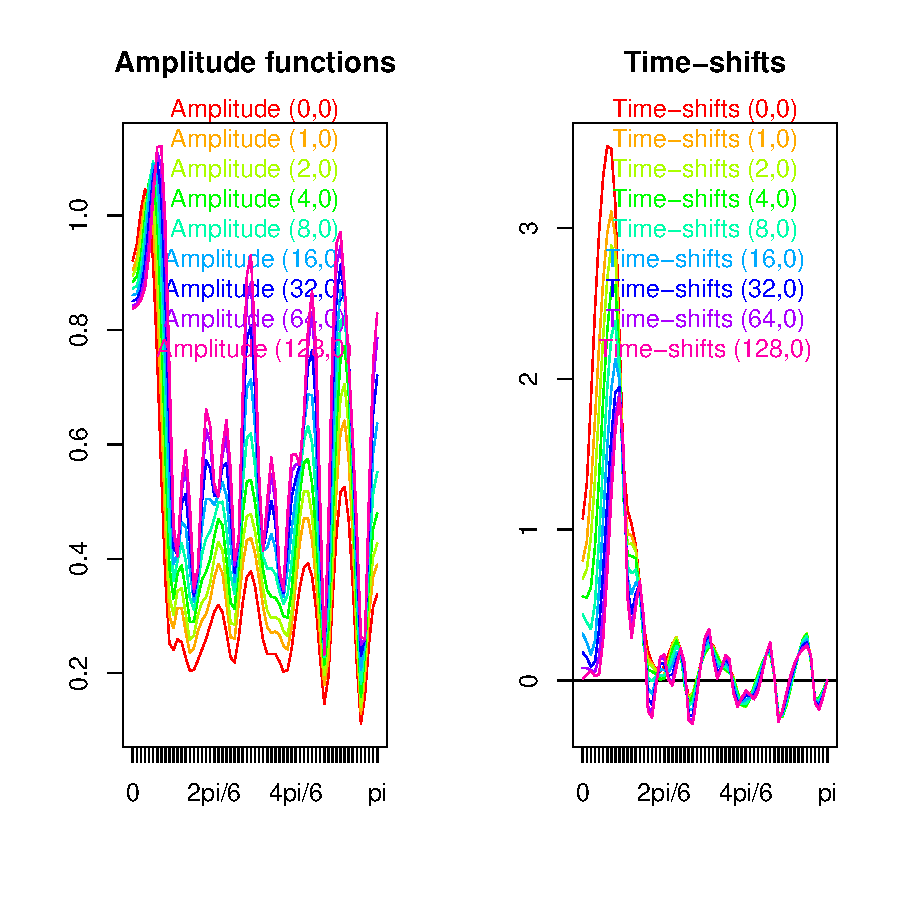
\includegraphics[height=3in, width=6in]{z_box_plot_amp_and_shift_cust_T_1}\caption{Amplitude (left) and time-shift functions (right) as a function of lambda for fixed eta=0\label{z_box_plot_amp_and_shift_cust_T_1}}\end{center}\end{figure}\item Filter-outputs are plotted in fig.\ref{z_dfa_cust_ats_out_1_T}: series are standardized in order to facilitate visual inspection.
\begin{figure}[H]\begin{center}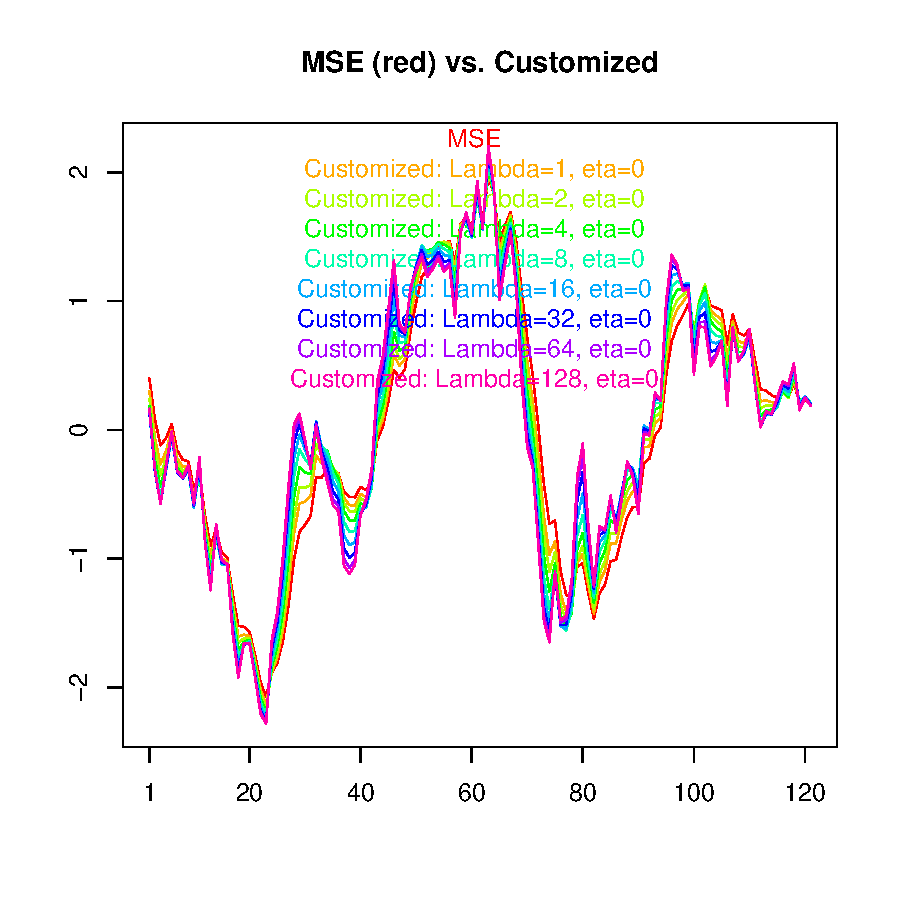
\includegraphics[height=3in, width=6in]{z_dfa_cust_ats_out_1_T}\caption{Filter outputs: MSE (red) vs. customized , a1=0.9\label{z_dfa_cust_ats_out_1_T}}\end{center}\end{figure}
\end{enumerate}



\subsubsection{Analysis}
\begin{itemize}
\item Accuracy, Timeliness and Smoothness sum-up to total MSE in table \ref{ats_comp_dfa_T}. Residual vanishes because the target filter vanishes in the stopband.
\item Timeliness decreases with increasing $\lambda$, as desired. Accuracy and Smoothness as well as total MSE increase, as a consequence.
\item Amplitude and time-shift functions in fig.\ref{z_box_plot_amp_and_shift_cust_T_1} provide more insights. Timeliness decreases because the time-shift is uniformly decreasing in the passband, as a function of $\lambda$. Accuracy increases with increasing $\lambda$ because the amplitude function departs from the target ($\Gamma(\omega)$ in the stopband: leakage is increasing with $\lambda$. As a consequence, Smoothness deteriorates. 
\item Outputs of the customized filter in fig.\ref{z_dfa_cust_ats_out_1_T} tend to lie to the left (they are `faster') and the series are becoming increasingly noisy, as $\lambda$ increases.
\end{itemize}


\subsection{Smoothness Only: $\eta\geq 0$, $\lambda=0$ Fixed}\label{smoo_on}



\begin{enumerate}
\item We fix $\lambda=0$ (no emphasis of Timeliness) and let $\eta=k*0.3, k=0,...,6$ (Smoothness is emphasized).
\begin{Schunk}
\begin{Sinput}
> # Specify the etas
> eta_vec<-0.3*0:6
> # Specify the fixed lambda
> lambda_vec<-rep(0,length(eta_vec))
\end{Sinput}
\end{Schunk}
\begin{Schunk}
\begin{Sinput}
> # Proceed to estimation
> for_sim_obj<-for_sim_out(a_vec,len1,len,cutoff,L,mba,estim_MBA,L_sym,
+              Lag,i1,i2,scaled_ATS,lambda_vec,eta_vec,anzsim,M,dif)
\end{Sinput}
\end{Schunk}

\item ATS-components and MSE for the first process ($a_1=0.9$) are summarized in table \ref{ats_comp_dfa_S}.
% latex table generated in R 3.3.2 by xtable 1.8-2 package
% Fri Dec 16 15:21:00 2016
\begin{table}[ht]
\centering
\begin{tabular}{rrrrrr}
  \hline
 & Accuracy & Timeliness & Smoothness & Residual & Total MSE \\ 
  \hline
DFA-MSE & 0.002282 & 0.016112 & 0.022069 & 0.000000 & 0.040463 \\ 
  Lambda=0, eta=0.3 & 0.003504 & 0.023179 & 0.016156 & 0.000000 & 0.042838 \\ 
  Lambda=0, eta=0.6 & 0.005257 & 0.031747 & 0.012262 & 0.000000 & 0.049266 \\ 
  Lambda=0, eta=0.9 & 0.007819 & 0.041832 & 0.009555 & 0.000000 & 0.059207 \\ 
  Lambda=0, eta=1.2 & 0.011606 & 0.053695 & 0.007473 & 0.000000 & 0.072774 \\ 
  Lambda=0, eta=1.5 & 0.017056 & 0.067872 & 0.005682 & 0.000000 & 0.090609 \\ 
  Lambda=0, eta=1.8 & 0.024362 & 0.084845 & 0.004081 & 0.000000 & 0.113288 \\ 
   \hline
\end{tabular}
\caption{ATS-Components as a function of eta (lambda=0 fixed)} 
\label{ats_comp_dfa_S}
\end{table}\item Amplitude and time-shift functions for the first process are plotted in fig.\ref{z_box_plot_amp_and_shift_cust_S_1}.
\begin{figure}[H]\begin{center}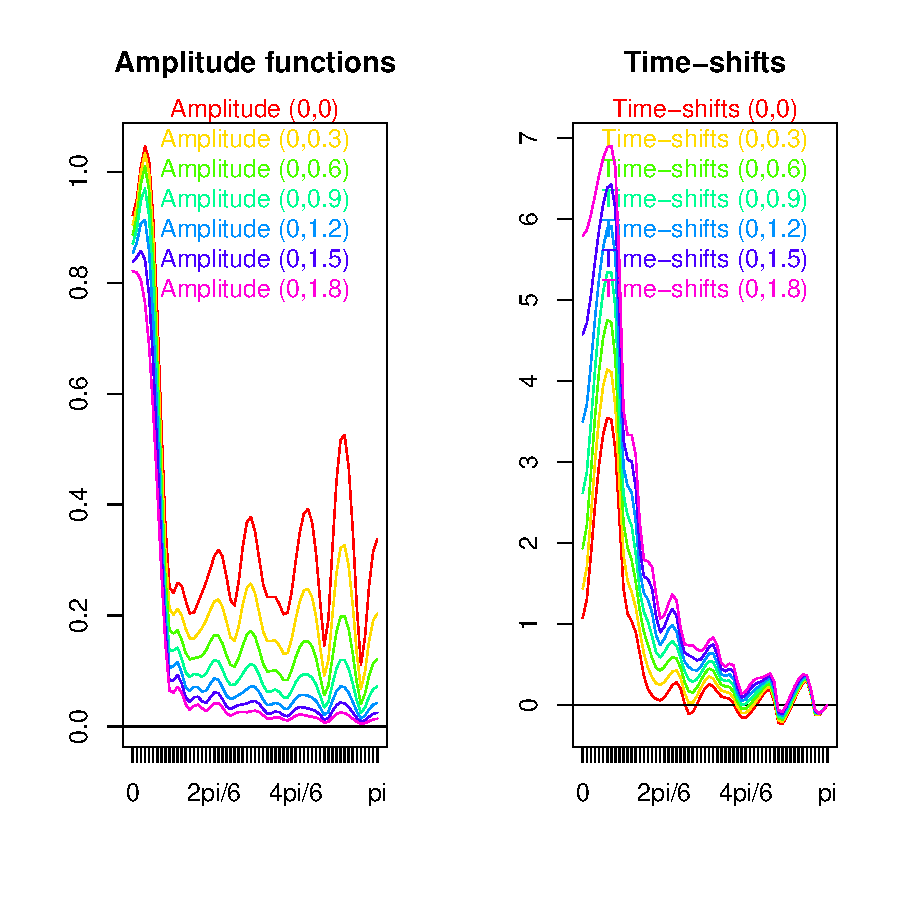
\includegraphics[height=3in, width=6in]{z_box_plot_amp_and_shift_cust_S_1}\caption{Amplitude (left) and time-shift functions (right) as a function of eta (lambda=0 fixed)\label{z_box_plot_amp_and_shift_cust_S_1}}\end{center}\end{figure}\item Filter coefficients can be seen in fig.\ref{z_box_plot_coef_S_1}.
\begin{figure}[H]\begin{center}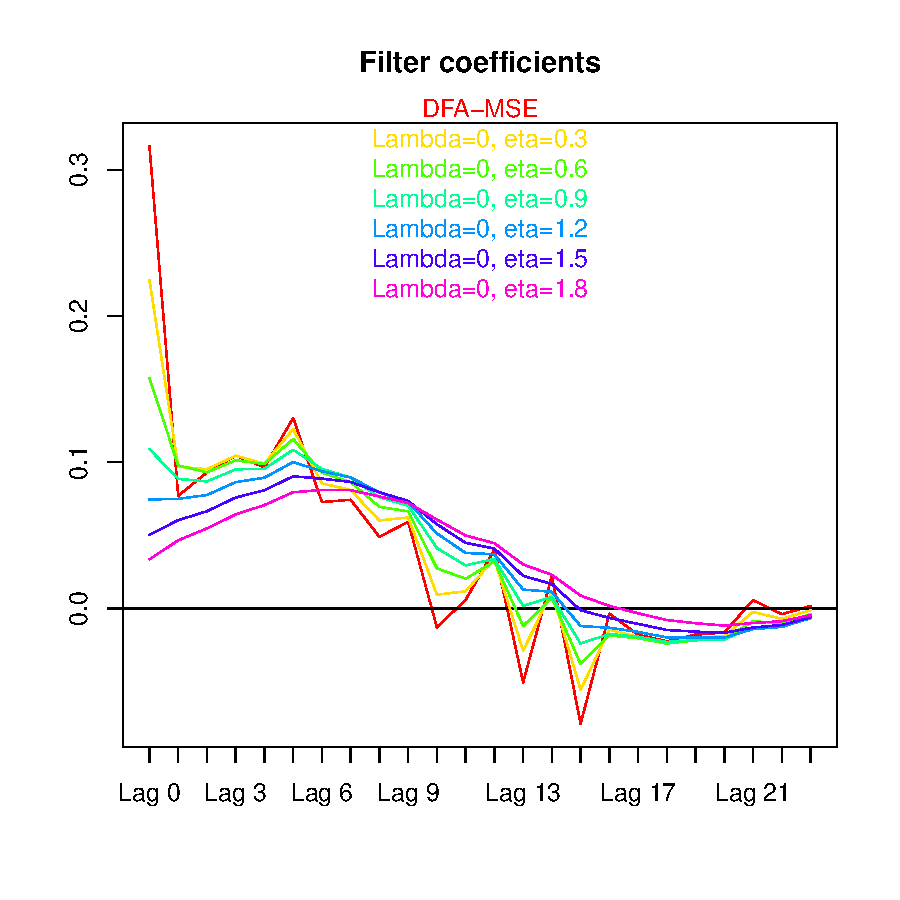
\includegraphics[height=3in, width=4in]{z_box_plot_coef_S_1}\caption{Filter coefficients as a function of eta (lambda=0 fixed)\label{z_box_plot_coef_S_1}}\end{center}\end{figure}\item Filter-outputs  are plotted in fig.\ref{z_dfa_cust_ats_out_1_S}: the series are standardized for ease of visual inspection.
\begin{figure}[H]\begin{center}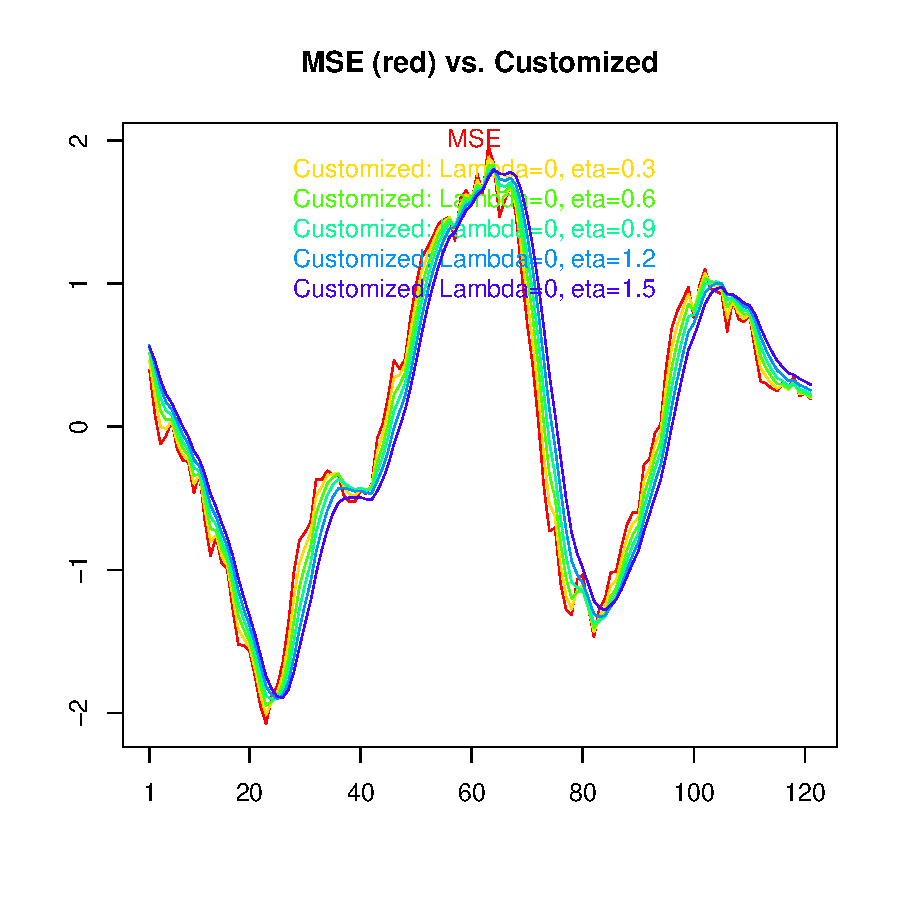
\includegraphics[height=3in, width=4in]{z_dfa_cust_ats_out_1_S}\caption{Filter outputs MSE (red) vs. customized, a1=0.9\label{z_dfa_cust_ats_out_1_S}}\end{center}\end{figure}

\end{enumerate}


\subsubsection{Analysis}
\begin{itemize}
\item Smoothness in table \ref{ats_comp_dfa_S} decreases with increasing $\eta$, as required. Accuracy, Timeliness as well as total MSE increase, as a consequence.
\item Amplitude and time-shift functions in fig.\ref{z_box_plot_amp_and_shift_cust_S_1} offer a more detailed picture: for increasing $\eta$ the amplitude functions are approaching zero in the stopband at costs of the time-shifts which grow substantially in the passband. 
\item Fig.\ref{z_box_plot_coef_S_1} reveals that filter coefficients become smoother for increasing $\eta$. This desirable side-effect is obtained by imposing stronger shrinkage of the amplitude function in the (wide) stopband: degrees of freedom are implicitly freezed; in particular, we expect overfitting to be contained. 
\item As $\eta$ increases, outputs of the customized filter in fig.\ref{z_dfa_cust_ats_out_1_S} tend to lie to the right (delay) and the series appear to be increasingly smooth.
\end{itemize}



\subsection{Emphasizing Timeliness and Smoothness: $\lambda,\eta\geq0$}\label{l_e_geq_0}




\begin{enumerate}
\item We compare the MSE-design $\lambda=\eta=0$ with the strongly customized filter $\lambda=128,\eta=1.8$ which emphasizes Timeliness and Smoothness simultaneously.
\begin{Schunk}
\begin{Sinput}
> # Specify the etas
> eta_vec<-c(0,1.8)
> # Specify the fixed lambda
> lambda_vec<-c(0,128)
\end{Sinput}
\end{Schunk}
\begin{Schunk}
\begin{Sinput}
> # Proceed to estimation
> for_sim_obj<-for_sim_out(a_vec,len1,len,cutoff,L,mba,estim_MBA,L_sym,
+               Lag,i1,i2,scaled_ATS,lambda_vec,eta_vec,anzsim,M,dif)
\end{Sinput}
\end{Schunk}

\item ATS-components and MSE for the first process ($a_1=0.9$) are summarized in table \ref{ats_comp_dfa_ST_1}.
% latex table generated in R 3.3.2 by xtable 1.8-2 package
% Fri Dec 16 15:21:01 2016
\begin{table}[ht]
\centering
\begin{tabular}{rrrrrr}
  \hline
 & Accuracy & Timeliness & Smoothness & Residual & Total MSE \\ 
  \hline
DFA-MSE & 0.002282 & 0.016112 & 0.022069 & 0.000000 & 0.040463 \\ 
  Lambda=128, eta=1.8 & 0.461697 & 0.000650 & 0.002427 & 0.000000 & 0.464774 \\ 
   \hline
\end{tabular}
\caption{ATS-Components as a function of lambda and eta, a1=0.9} 
\label{ats_comp_dfa_ST_1}
\end{table}

\item Amplitude and time-shift functions for the first process are plotted in fig.\ref{z_box_plot_amp_and_shift_cust_ST_1}.
\begin{figure}[H]\begin{center}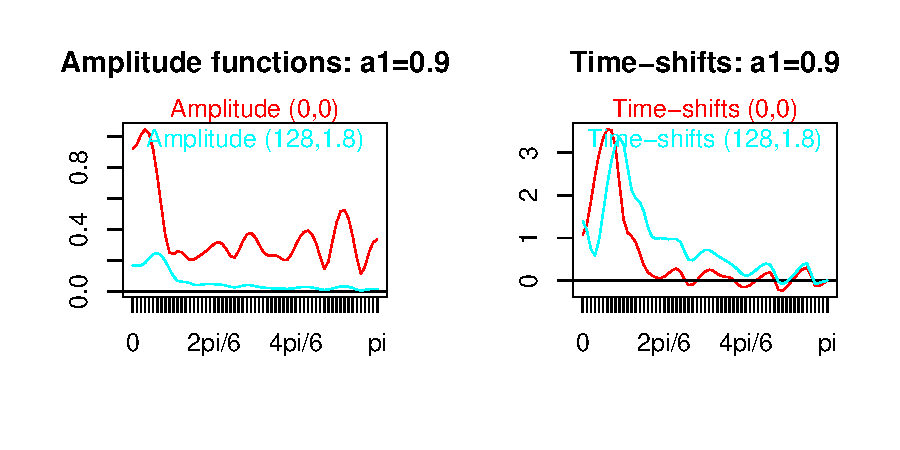
\includegraphics[height=3in, width=4in]{z_box_plot_amp_and_shift_cust_ST_1}\caption{Amplitude (left) and time-shift functions (right) as a function of lambda and eta\label{z_box_plot_amp_and_shift_cust_ST_1}}\end{center}\end{figure}\item Filter-outputs of MSE and customized  filters are plotted in fig.\ref{z_dfa_cust_ats_out_1_ST} (series are standardized for ease of visual inspection).
\begin{figure}[H]\begin{center}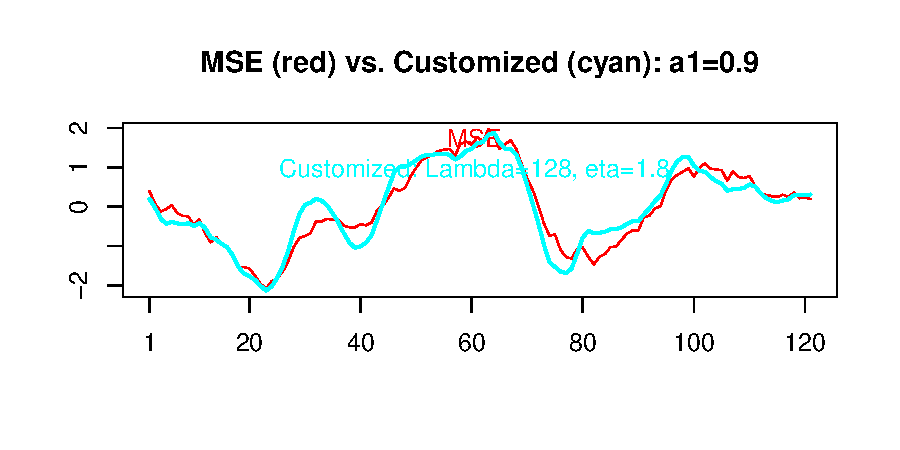
\includegraphics[height=3in, width=4in]{z_dfa_cust_ats_out_1_ST}\caption{Filter outputs MSE (red) vs. customized (cyan), a1=0.9\label{z_dfa_cust_ats_out_1_ST}}\end{center}\end{figure}

\end{enumerate}


\subsubsection{Analysis}
\begin{itemize}
\item As confirmed in table \ref{ats_comp_dfa_ST_1}, the customized design improves in terms of Timeliness as well as of Smoothness, {simultaneously} at costs of a remarkable deterioration of Accuracy and, as a a consequence, of total MSE.
\item The time-shift of the customized design in fig.\ref{z_box_plot_amp_and_shift_cust_ST_1} is generally smaller in the passband (except at frequency zero). Its amplitude function is close to zero in the passband, as desired;  but the amplitude of the customized filter is also pulled towards zero in the passband (zero-shrinkage of the coefficients) which explains the excess Accuracy- and MSE-losses.   
\item The output of the customized filter in fig.\ref{z_dfa_cust_ats_out_1_ST} tends to lie to the left (faster) and it is smoother, as desired (recall that the series are standardized).
\end{itemize}
In order to grasp the observed zero-shrinkage of the customized filter we observe that  the scale-dependent Timeliness and Smoothness measures vanish if the amplitude function shrinks to zero. Accuracy alone lifts the amplitude away from zero (at least in the passband). Therefore, emphasizing heavily Smoothness and Timeliness, as we did in our example, exhausts to some extent Accuracy's action\footnote{The supernumerary amplitude-term in criterion \ref{idfatp} is counterproductive too, see section \ref{idfas}.}. Fortunately, this problem could be addressed by a simple re-scaling of the (customized) filter output\footnote{Recall that the series in fig.\ref{z_dfa_cust_ats_out_1_ST} were standardized.}, as we briefly explore below. 
\begin{Schunk}
\begin{Sinput}
> # We allow for a re-calibration (by the inverse amplitude function in the passband)
> scaled_ATS<-T
> for_sim_obj<-for_sim_out(a_vec,len1,len,cutoff,L,mba,estim_MBA,L_sym,Lag,i1,
+                         i2,scaled_ATS,lambda_vec,eta_vec,anzsim,M,dif)
\end{Sinput}
\end{Schunk}
Specifically, we scale the filter coefficients by a constant which is inversely proportional to the  amplitude function in the passband\footnote{Alternatively one could fit an optimal MSE-normalization.}
\[
\textrm{Calibration~term}:=\frac{\textrm{Length~of~passband}}{\sum_{\textrm{Passband}}\hat{A}(\omega_k)}
\]
Fig. \ref{z_box_plot_amp_and_shift_cust_ST_1_scaled_unscaled} and table \ref{ats_comp_dfa_ST_1_scaled_unscaled} confirm that the previous zero-shrinkage is withdrawn.
\begin{figure}[H]\begin{center}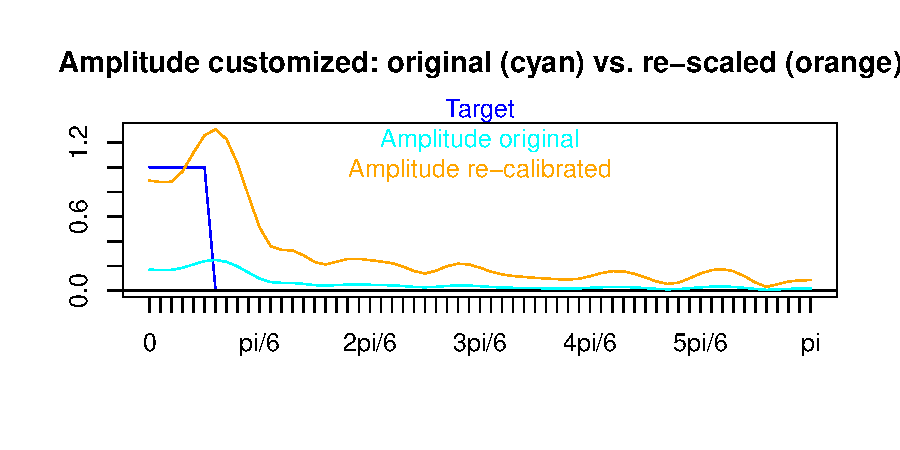
\includegraphics[height=4in, width=4in]{z_box_plot_amp_and_shift_cust_ST_1_scaled_unscaled}\caption{Amplitude functions of original (cyan) and scaled customized filter (orange)\label{z_box_plot_amp_and_shift_cust_ST_1_scaled_unscaled}}\end{center}\end{figure}In particular, Accuracy and MSE are relaxed, this time at costs of Smoothness and Timeliness.  
% latex table generated in R 3.3.2 by xtable 1.8-2 package
% Fri Dec 16 15:21:02 2016
\begin{table}[ht]
\centering
\begin{tabular}{rrrrrr}
  \hline
 & Accuracy & Timeliness & Smoothness & Residual & Total MSE \\ 
  \hline
Customized unscaled & 0.461697 & 0.000650 & 0.002427 & 0.000000 & 0.464774 \\ 
  Customized re-scaled & 0.008751 & 0.003422 & 0.067254 & 0.000000 & 0.079428 \\ 
   \hline
\end{tabular}
\caption{ATS-Components of customized design: unscaled vs. scaled filter, a1=0.9} 
\label{ats_comp_dfa_ST_1_scaled_unscaled}
\end{table}We retain from the above examples that both the time-shift (delay) as well as the noise-suppression of a (real-time) filter can be addressed by a decomposition of the MSE-norm into ATS-components. However, The fact that Timeliness and Smoothness are scale-dependent measures hampers interpretability. Therefore we now propose an alternative set of scale-invariant measures which will allow for a straightforward evaluation of customized designs. 









\section{Curvature and Peak-Correlation}\label{peco_cu}

\subsection{Definition}

Define
\begin{eqnarray}\label{mse_2diff}
\textrm{Curvature}&:=&\frac{E\left[\Big((1-B)^2 \widehat{y}_t\Big)^2\right]}{\textrm{var}(\widehat{y_t})}\\
\label{peak_corr}
\textrm{Peak-Correlation}&:=&\textrm{Arg}\left(\max_j(cor(y_t,\widehat{y}_{t+j}))\right)
\end{eqnarray}
where $(1-B)^2$ is the second-order difference operator (curvature) and where $\textrm{Arg}\left(\max_j(cor(y_t,\widehat{y}_{t+j}))\right)$ means the lead or lag $j_0$ at which the correlation between the target $y_t$ and the estimate $\hat{y}_{t+j_0}$ is maximized\footnote{In applications, $y_t$ is generally unobserved and must be approximated by symmetric filters of finite order. Fortunately, the Peak Correlation concept is fairly robust against such approximations because the effective value of the correlation is irrelevant since we are solely interested in the lead/lag at which the correlation peaks.}. Note also that the covariance could be substituted to the correlation without altering the corresponding outcome.  Curvature and Peak Correlation are scale-invariant measures. As we shall show, they are linked to Smoothness and Timeliness. Empirical measures can be obtained by substituting  sample-estimates for unknown expectations in the above expressions. 


\subsection{Examples}  

We apply the above statistics to our previous example and complete the former tables \ref{ats_comp_dfa_T} (emphasizing Timeliness only), \ref{ats_comp_dfa_S} (emphasizing Smoothness only) and \ref{ats_comp_dfa_ST_1} (emphasizing Timeliness and Smoothness). 
% latex table generated in R 3.3.2 by xtable 1.8-2 package
% Fri Dec 16 15:21:02 2016
\begin{table}[ht]
\centering
\begin{tabular}{rrrrrrrr}
  \hline
 & Accuracy & Timeliness & Smoothness & Residual & Total MSE & Curv-in & Peak-Cor-in \\ 
  \hline
DFA-MSE & 0.002282 & 0.016112 & 0.022069 & 0.000000 & 0.040463 & 0.053264 & 2.000000 \\ 
  Lambda=1, eta=0 & 0.004020 & 0.008884 & 0.030273 & 0.000000 & 0.043177 & 0.076929 & 2.000000 \\ 
  Lambda=2, eta=0 & 0.005359 & 0.005849 & 0.035979 & 0.000000 & 0.047186 & 0.093906 & 1.000000 \\ 
  Lambda=4, eta=0 & 0.007217 & 0.003298 & 0.043450 & 0.000000 & 0.053966 & 0.117728 & 1.000000 \\ 
  Lambda=8, eta=0 & 0.009367 & 0.001653 & 0.051885 & 0.000000 & 0.062905 & 0.147909 & 0.000000 \\ 
  Lambda=16, eta=0 & 0.011534 & 0.000755 & 0.060728 & 0.000000 & 0.073016 & 0.183068 & 0.000000 \\ 
  Lambda=32, eta=0 & 0.013509 & 0.000306 & 0.069476 & 0.000000 & 0.083291 & 0.219062 & 0.000000 \\ 
  Lambda=64, eta=0 & 0.015105 & 0.000109 & 0.077027 & 0.000000 & 0.092241 & 0.249550 & 0.000000 \\ 
  Lambda=128, eta=0 & 0.016246 & 0.000036 & 0.082459 & 0.000000 & 0.098740 & 0.270883 & 0.000000 \\ 
   \hline
\end{tabular}
\caption{ATS-Components, Peak-Correlation and Curvature: emphasizing Timeliness only, a1=0.9} 
\label{ats_comp_dfa_T_1_pc}
\end{table}\begin{itemize}
\item In table \ref{ats_comp_dfa_T_1_pc} Timeliness as well as Peak-Correlation decrease with increasing $\lambda$, as desired. The Peak Correlation is readily interpretable: in particular target series and real-time estimate appear to be  synchronized for $\lambda\geq 8$ (Peak Correlation vanishes).
% latex table generated in R 3.3.2 by xtable 1.8-2 package
% Fri Dec 16 15:21:02 2016
\begin{table}[ht]
\centering
\begin{tabular}{rrrrrrrr}
  \hline
 & Accuracy & Timeliness & Smoothness & Residual & Total MSE & Curv-in & Peak-Cor-in \\ 
  \hline
DFA-MSE & 0.002282 & 0.016112 & 0.022069 & 0.000000 & 0.040463 & 0.053264 & 2.000000 \\ 
  Lambda=0, eta=0.3 & 0.003504 & 0.023179 & 0.016156 & 0.000000 & 0.042838 & 0.023755 & 3.000000 \\ 
  Lambda=0, eta=0.6 & 0.005257 & 0.031747 & 0.012262 & 0.000000 & 0.049266 & 0.010688 & 3.000000 \\ 
  Lambda=0, eta=0.9 & 0.007819 & 0.041832 & 0.009555 & 0.000000 & 0.059207 & 0.004966 & 4.000000 \\ 
  Lambda=0, eta=1.2 & 0.011606 & 0.053695 & 0.007473 & 0.000000 & 0.072774 & 0.002446 & 5.000000 \\ 
  Lambda=0, eta=1.5 & 0.017056 & 0.067872 & 0.005682 & 0.000000 & 0.090609 & 0.001301 & 5.000000 \\ 
  Lambda=0, eta=1.8 & 0.024362 & 0.084845 & 0.004081 & 0.000000 & 0.113288 & 0.000748 & 6.000000 \\ 
   \hline
\end{tabular}
\caption{ATS-Components, Peak-Correlation and Curvature: emphasizing Smoothness only, a1=0.9} 
\label{ats_comp_dfa_S_1_pc}
\end{table}\item In table \ref{ats_comp_dfa_S_1_pc} Smoothness and Curvature decline with increasing $\eta$, as desired. The latter is readily interpretable in terms of normalized (inverse) signal-to-noise ratio. As a trade off, the Peak Correlation increases substantially. 
% latex table generated in R 3.3.2 by xtable 1.8-2 package
% Fri Dec 16 15:21:02 2016
\begin{table}[ht]
\centering
\begin{tabular}{rrrrrrrr}
  \hline
 & Accuracy & Timeliness & Smoothness & Residual & Total MSE & Curv-in & Peak-Cor-in \\ 
  \hline
DFA-MSE & 0.002282 & 0.016112 & 0.022069 & 0.000000 & 0.040463 & 0.053264 & 2.000000 \\ 
  Lambda=128, eta=1.8 & 0.461697 & 0.000650 & 0.002427 & 0.000000 & 0.464774 & 0.016443 & 0.000000 \\ 
  Scaled customized & 0.008751 & 0.003422 & 0.067254 & 0.000000 & 0.079428 & 0.016443 & 0.000000 \\ 
   \hline
\end{tabular}
\caption{ATS-Components, Peak-Correlation and Curvature: emphasizing Timeliness and Smoothness, a1=0.9} 
\label{ats_comp_dfa_ST_1_pc}
\end{table}\item In table \ref{ats_comp_dfa_ST_1} the double-score of the customized design is evidenced by Peak Correlation and Curvature which remain unaffected by the normalization (last row), in contrast to Timeliness and Smoothness.      
\end{itemize}
We deduce from the above examples that the new Peak Correlation and Curvature statistics are simple to implement, simple to formalize and simple to interpret.


\subsection{Linking ATS-Components, Peak Correlation and Curvature}


Consider the second-order differences in the numerator of the Curvature statistic \ref{mse_2diff}

\begin{eqnarray*}
E\left[\Big((1-B)^2 \widehat{y}_t\Big)^2\right]&\approx&\frac{1}{T}\sum_{t=1}^T \left\{(1-B)^2 \widehat{y}_t\right\}^2\\
&=&\frac{2\pi}{T}\sum_{\textrm{All~frequencies}}I_{T\Delta^2\hat{Y}}(\omega_k)\\
&\approx&\frac{2\pi}{T}\sum_{\textrm{All~frequencies}}|1-\exp(-i\omega_k)|^4I_{T\hat{Y}}\\
&\approx&\frac{2\pi}{T}\sum_{\textrm{All~frequencies}}|1-\exp(-i\omega_k)|^4\hat{A}^2(\omega_k)I_{TX}
\end{eqnarray*}
where we assumed that $\hat{y}_{-1},\hat{y}_0$ were available and where $I_{T\Delta^2\hat{Y}}(\omega_k)$ is the periodogram of $(1-B)^2 \widehat{y}_t$. The first equality follows from \ref{spec_dec_per} and the subsequent approximations follow from \ref{conv_per}.\\
We can compare this expression to  Smoothness
\[S=\frac{2\pi}{ T} \sum_{\textrm{Stopband}} \hat{A}(\omega_k)^2 W(\omega_k,\eta) I_{TX}(\omega_k)\]
which is defined in the stopband, only. Assimilating $|1-\exp(-i\omega_k)|^4$ with $W(\omega_k,\eta)$ and ignoring the passband establishes a link between Curvature and Smoothness\footnote{Note also that we ignored the denominator $\textrm{var}(\widehat{y_t})$ in the Curvature expression: the latter ensures scale-invariance of the measure.}.\\

In order to relate Peak Correlation to Timeliness we consider the following development\footnote{Recall that the covariance could be substituted to the correlation without affecting numbers i.e. Peak Correlation and Peak Covariance are identical statistics.}
\begin{eqnarray*}
cov(y_t,\widehat{y}_{t+j})&\approx&\frac{1}{T}\sum_{t=1}^Ty_t\hat{y}_{t+j}\\
&\approx&\frac{2\pi}{T}\sum_{\textrm{All~frequencies}} \Re\left(\Xi_{TY}(\omega_k)\overline{\exp(ij\omega_k)\Xi_{T\hat{Y}}(\omega_k)}\right)\\
&\approx&\frac{2\pi}{T}\sum_{\textrm{All~frequencies}}\Re\left(\Gamma(\omega_k)\Xi_{TX}(\omega_k)\overline{\exp(ij\omega_k)\hat{\Gamma}(\omega_k)\Xi_{TX}(\omega_k)}\right)\\
&=&\frac{2\pi}{T}\sum_{\textrm{Passband}}A(\omega_k)\hat{A}(\omega_k) \Re\left(\overline{\exp(ij\omega_k-i\hat{\Phi}(\omega_k))}\right)I_{TX}(\omega_k)\\
&=&\frac{2\pi}{T}\sum_{\textrm{Passband}}A(\omega_k)\hat{A}(\omega_k) \cos(j\omega_k-\hat{\Phi}(\omega_k))I_{TX}(\omega_k)
\end{eqnarray*}
The second approximation is a consequence of proposition \ref{convolution theorem} in \ref{dis_con_app}. Let's assume, for a while, that $j$ is not a fixed integer but a general real-valued function of $\omega_k$. Then the last term in the above development would be maximized, as a function of $j(\omega_k)$, if $j(\omega_k)=\hat{\Phi}(\omega_k)/\omega_k=\hat{\phi}(\omega_k)$ (up to multiples of $2\pi$).  Therefore, reducing the time-shift $\hat{\phi}(\omega_k)$ in the passband, by emphasizing Timeliness, will decrease the lag at which the covariance or the correlation are peaking, which formalizes the link between Peak Correlation and Timeliness. 





\section{Double Score Against the MSE Paradigm}\label{double_score_ats}



\subsection{Introduction}

We here illustrate the flexibility of the ATS-trilemma by benchmarking empirical real-time designs (nowcasts), optimized in view of particular research priorities (speed/reliability), against the best theoretical \emph{MSE}-filter, assuming knowledge of the \emph{true DGP}. The empirical framework leans on the previous sections, see McElroy and Wildi (2015), and the whole R-code is carried over. In contrast to the previous sections, where we emphasized \emph{single} realization \emph{in-sample} results, we now consider \emph{multiple} realizations and compute in-sample as well as \emph{out-of-sample} {distributions} of performance measures of competing designs. Specifically, we analyze performances based on the classic (total) MSE-norm as well as on the scale-invariant Peak Correlation and Curvature measures introduced in the previous section. \\

Our contenders in this study will be the best theoretical MSE-estimate based on knowledge of the true DGP (benchmark), as well as the following empirical designs
\begin{itemize}
\item DFA-MSE: $\lambda=\eta=0$
\item Strong noise suppression: $\lambda=0,\eta=1.5$
\item Balanced (fast and smooth): $\lambda=30,\eta=1$
\item Very fast: $\lambda=500,\eta=0.3$
\end{itemize}



\subsection{Simulation Run}





Coefficients of the benchmark MSE-filters can be obtained by substituting the true spectral density
\[\left|\frac{\sigma^2}{1-a_1\exp(-i\omega)}\right|^2~,~a_1=-0.9,0.1,0.9\]
for the periodogram $I_{TX}(\omega)$ in \ref{dfatp}, setting $\lambda=\eta=0$, see chapter \ref{rep_sec} for further background\footnote{We implement an alternative time-domain solution in our R-code, see chapter \ref{rep_sec}.}. Note that benchmark filters do not depend on data, at all. Our target filter is the ideal trend with cutoff $\pi/12$.  
For the empirical DFA-filters we generate 100 realizations for each process and compute real-time (nowcast) filters of length $L=24$. The code leans on McElroy and Wildi (2015)\footnote{It is a faster-running `debugged' version based on reconciliation with a multivariate extension proposed in the next section.}:
\begin{enumerate}
\item Source the R-file
\begin{Schunk}
\begin{Sinput}
> source(file=paste(path.pgm,"functions_trilemma.r",sep=""))
\end{Sinput}
\end{Schunk}
The functions in this file generate the data, estimate filter coefficients, compute performance measures (in- and out-of-sample), ATS-components as well as amplitude and time-shift-functions. 
\item Specify the empirical design (same as in the previous section except for the number of realizations) and run the code. 
\begin{Schunk}
\begin{Sinput}
> # Number of realizations
> anzsim<-100
\end{Sinput}
\end{Schunk}
\begin{Schunk}
\begin{Sinput}
> # Proceed to simulation run
> for_sim_obj<-for_sim_out(a_vec,len1,len,cutoff,L,mba,estim_MBA,L_sym,Lag,
+                       i1,i2,scaled_ATS,lambda_vec,eta_vec,anzsim,M,dif)
\end{Sinput}
\end{Schunk}
\end{enumerate}

\subsection{Analysis}


\subsubsection{Performance Measures}

In order to save space we emphasize the second process $a_1=0.1$\footnote{Recall that this model fits log-returns of INDPRO quite well over a longer historical time span.}. Fig.\ref{z_box_plot_emp_per_perf_inout_2}  shows box-plots of in-sample (left) and out-of-sample (right) Curvature and Peak Correlation performances and fig.\ref{z_box_plot_emp_per_perf_mse_inout_2}  shows the corresponding sample MSEs: the latter are \emph{effective} time-domain measures
\[\frac{1}{120}\sum_{t=1}^{120}(y_t-\hat{y}_t)^2\]
where the target signal $y_t$ is obtained by applying a high-order (finite) symmetric trend filter to (very) long time series. Plots of the other two processes are shown in  section \ref{app_double_score_ats} in the Appendix \ref{dstt}.


\begin{figure}[H]\begin{center}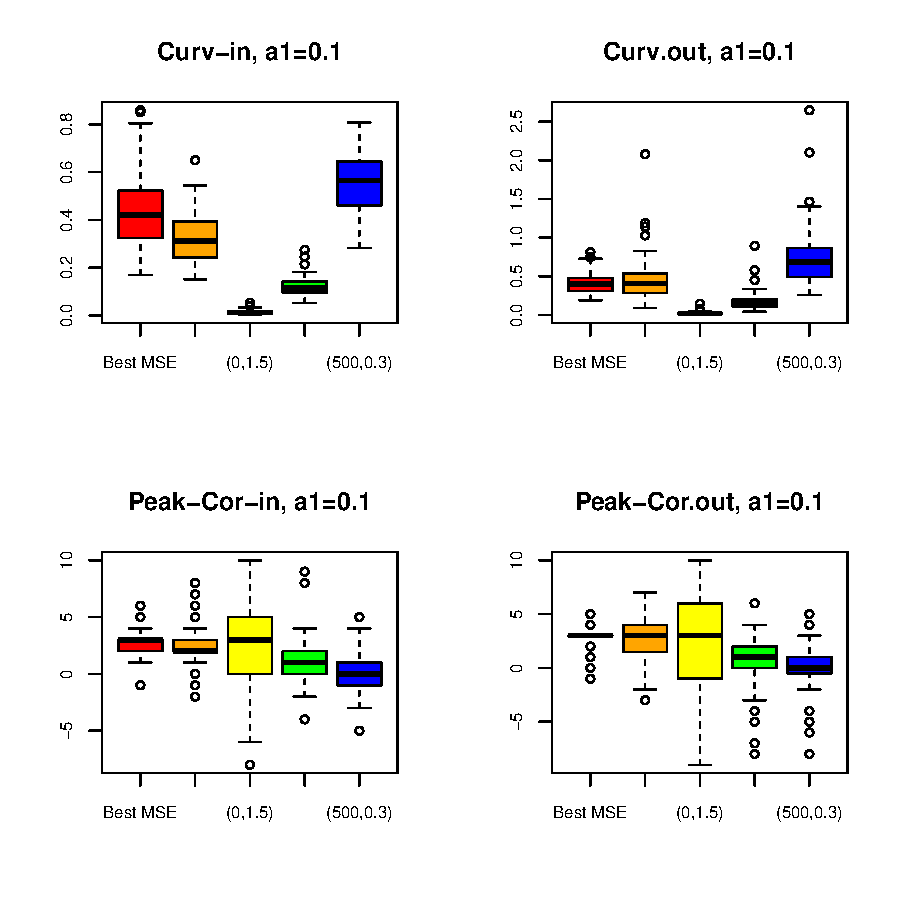
\includegraphics[height=5in, width=5in]{z_box_plot_emp_per_perf_inout_2}\caption{Empirical distributions
  of Curvature and Peak-Correlation of best theoretical MSE (red), empirical MSE (orange), strong noise suppression (yellow), balanced fast and smooth (green) and very fast (blue) filters. All empirical filters are based on the periodogram:
  in-sample (left plots) and out-of-sample (right plots) for a1=0.1\label{z_box_plot_emp_per_perf_inout_2}}\end{center}\end{figure}


\begin{figure}[H]\begin{center}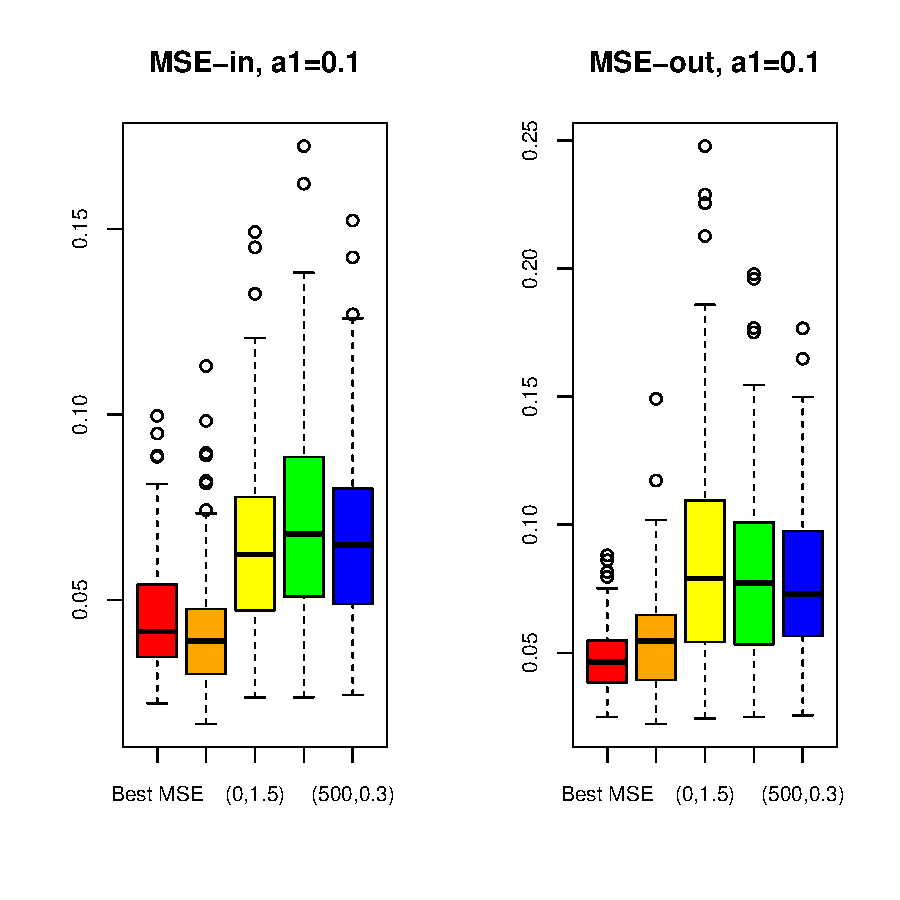
\includegraphics[height=2.5in, width=5in]{z_box_plot_emp_per_perf_mse_inout_2}\caption{Empirical distributions
  of Sample MSEs of best theoretical MSE (red), empirical MSE (orange), strong noise suppression (yellow), balanced fast and speed (green) and very fast (blue) filters. All empirical filters are based on the periodogram:
  in-sample (left plots) and out-of-sample (right plots) for a1=0.1\label{z_box_plot_emp_per_perf_mse_inout_2}}\end{center}\end{figure}
\textbf{Findings}
\begin{itemize}
\item The customized designs perform as expected. In particular the balanced design (green) outperforms the benchmark MSE-filter both in terms of Curvature as well as Peak-Correlation, in- and out-of-sample. 
\item In- and out-of-sample performances are congruent\footnote{The distributions of the integer-valued Peak Correlations are almost identical due, in part, to discretization effects.}.  
\item A comparison of in- and out-of-sample MSE-performances of benchmark (red) and empirical (orange) filters is indicative for overfitting: the orange filter performs slightly better in-sample but it is slightly outperformed out-of-sample. Interestingly, overfitting is moderate\footnote{In contrast to classic forecast approaches, which target an allpass filter, our examples target a lowpass filter with a wide stop-band. A close fit of the target in the stopband mimics, in some ways, classic shrinkage approaches or, stated otherwise, degrees of freedom are implicitly controlled by the DFA/MDFA-criteria.} even in the case of richly parametrized designs ($L=$24 coefficients are estimated in samples of length $T=$120).
\item The customized designs are systematically outperformed in terms of MSE-performances in- and out-of-sample, as expected. 
\end{itemize}




\subsubsection{Real-Time Filter Outputs}


Benchmark-MSE (red) and customized-balanced (green) filter-outputs are compared in fig.\ref{z_dfa_cust_ats_mba_per_e} (both time series are standardized for ease of visual inspection). The chosen time-span covers in-sample as well as out-of-sample periods. 

\begin{figure}[H]\begin{center}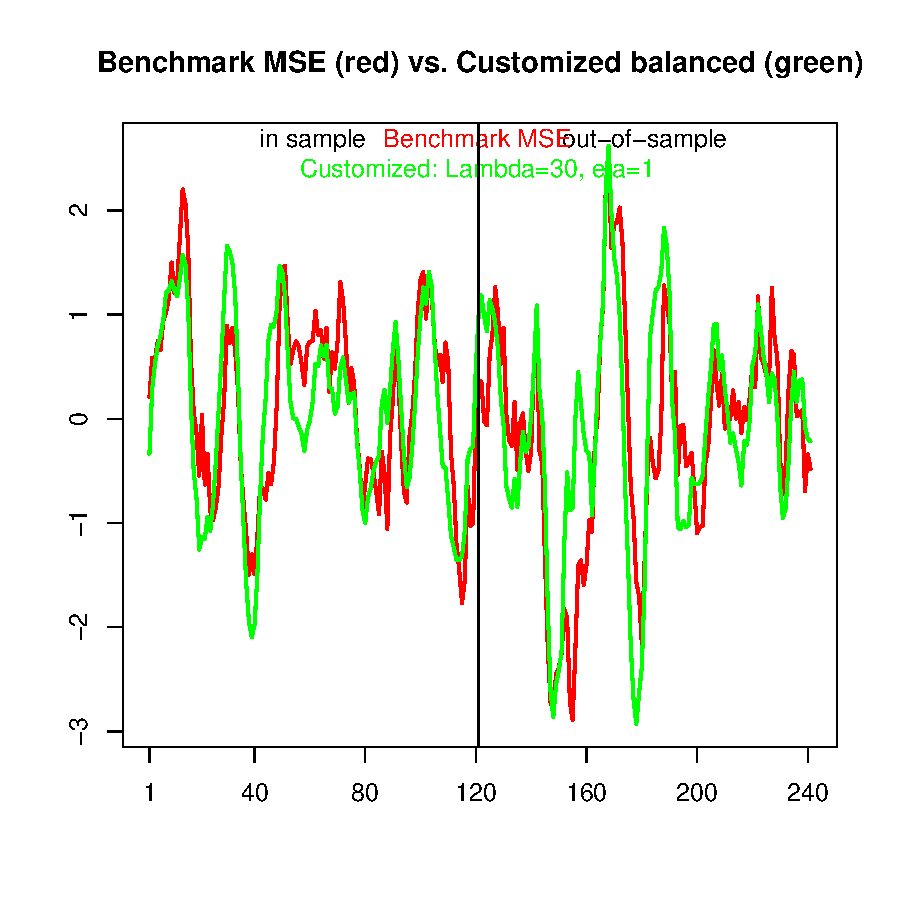
\includegraphics[height=4in, width=6in]{z_dfa_cust_ats_mba_per_e}\caption{Outputs of benchmark MSE (red) and customized balanced (green) filters: a1=0.1. In-sample (left half) and out-of-sample (right half)\label{z_dfa_cust_ats_mba_per_e}}\end{center}\end{figure}The customized filter outperforms the benchmark-MSE design on both accounts: it lies on the left (faster) and it is smoother both in-sample as well as out-of-sample. 







\section{Univariate Customized Design vs. Bivariate MSE Leading-Indicator}\label{ucdvbmseli}

In this section we stiffen the competition by benchmarking the univariate customized filter against a bivariate MSE-design with a leading indicator. The empirical design is otherwise identical to the previous section. 



\subsubsection{Data and Contenders}

We emphasize performances in the case of the second process ($a_1=0.1$) and compare the univariate MSE-DFA $\lambda=\eta=0$ (orange), the univariate balanced customized DFA $\lambda=30$,$\eta=1$ (green)) and the bivariate MDFA-MSE design proposed in section \ref{bimdfaudfa}.
\begin{Schunk}
\begin{Sinput}
> # Second process
> a1<-0.1
> # Customization settings DFA
> lambda_vec<-c(0,30)
> eta_vec<-c(0,1)
\end{Sinput}
\end{Schunk}
\begin{Schunk}
\begin{Sinput}
> # Run the competition: the new function handles the multivariate case
> cust_leading_obj<-mdfa_mse_leading_indicator_vs_dfa_customized(anzsim,
+                   a1,cutoff,L,lambda_vec,eta_vec,len1,len,i1,i2,Lag,
+                   lambda_mdfa,eta_mdfa,troikaner)  
\end{Sinput}
\end{Schunk}



\subsection{Performances: Curvature}

Box-plots of in-sample and out-of-sample Curvature-scores are depicted in fig.\ref{z_curv_dfacust_leadind}.
\begin{figure}[H]\begin{center}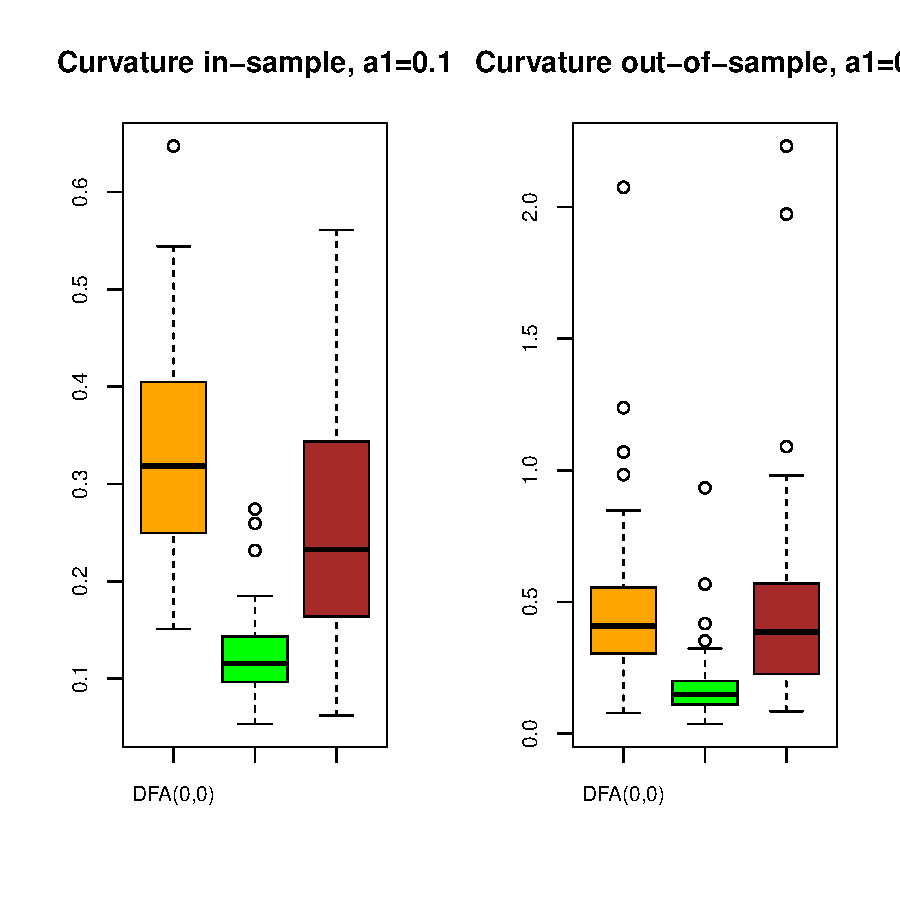
\includegraphics[height=3in, width=4in]{z_curv_dfacust_leadind}\caption{Curvature: mean-square DFA (orange), customized DFA (green) and MSE-MDFA leading indicator (brown): a1=0.1 In-sample (left) and out-of-sample (right).\label{z_curv_dfacust_leadind}}\end{center}\end{figure}The empirical distributions of the univariate designs coincide with those reported in the previous section (same random-seed). The customized design (green) outperforms both contenders in-sample as well as out-of-sample. In- and out-of-sample figures are remarkably similar considering that the bivariate design (brown) relies on 48 estimated coefficients, in realizations of length $T=$120, only. 



\subsection{Performances: Peak-Correlation}

Box-plots of in-sample and out-of-sample Peak-Correlation scores are shown in fig.\ref{z_peak_cor_dfacust_leadind}.

\begin{figure}[H]\begin{center}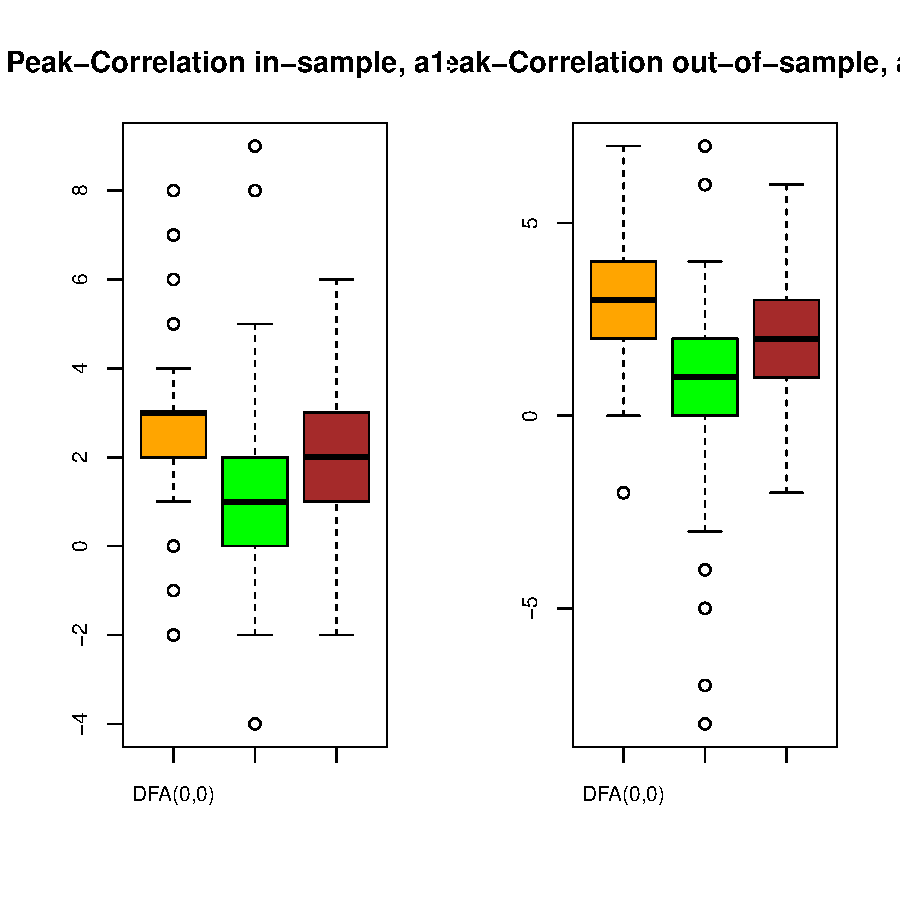
\includegraphics[height=3in, width=4in]{z_peak_cor_dfacust_leadind}\caption{Peak Correlation: mean-square DFA (orange), customized DFA (green) and MSE-MDFA leading indicator (brown): a1=0.1 In-sample (left) and out-of-sample (right).\label{z_peak_cor_dfacust_leadind}}\end{center}\end{figure}The customized design (green) substantially outperforms both contenders: it anticipates the DFA-MSE (orange) by -2 time-units in the median; remarkably, it also outperforms the leading-indicator design (brown) by -1 time-unit\footnote{Setting $\lambda=100$ would result in an anticipation of the customized design by 2 time-units, at costs of Accuracy and Smoothness.}. As expected, the univariate MSE-DFA (orange) is lagging the MSE-leading-indicator design (brown) by 1 time-unit which reflects the lead-time provided by  the additional leading indicator.




\subsection{Performances: MSE}


Box-plots of in-sample and out-of-sample MSE-scores are shown in fig.\ref{z_MSE_dfacust_leadind}.
\begin{figure}[H]\begin{center}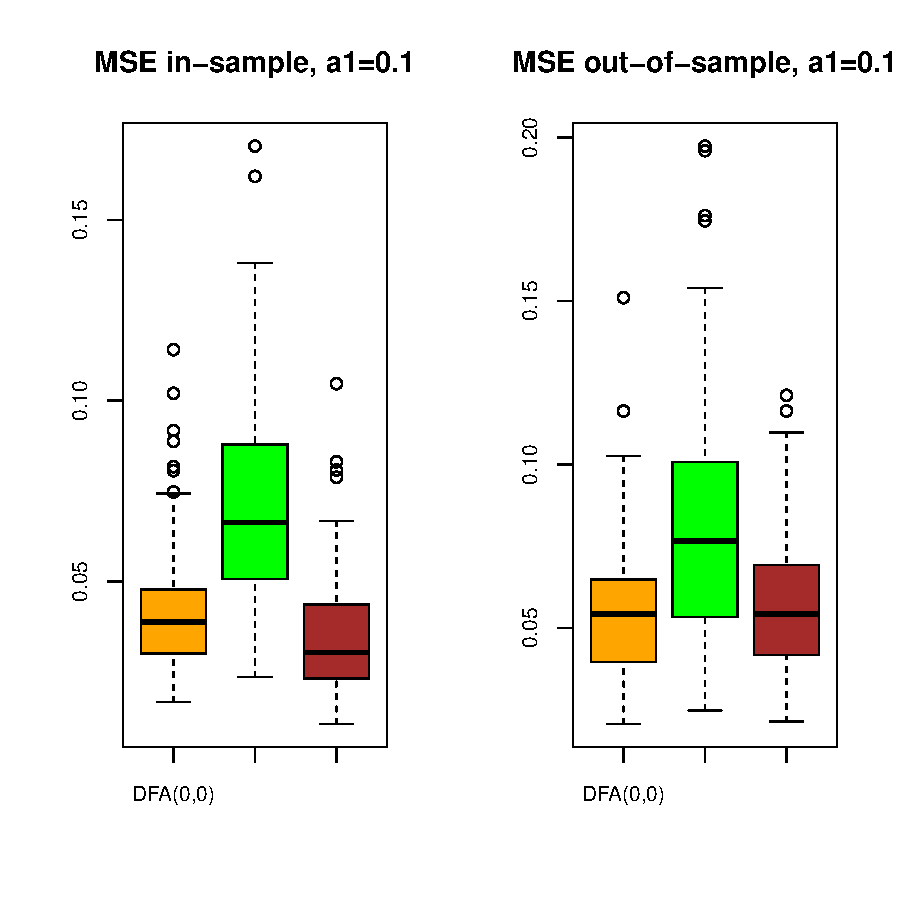
\includegraphics[height=3in, width=4in]{z_MSE_dfacust_leadind}\caption{MSE: mean-square DFA (orange), customized DFA (green) and MSE-MDFA leading indicator (brown): a1=0.1 In-sample (left) and out-of-sample (right).\label{z_MSE_dfacust_leadind}}\end{center}\end{figure}The customized design (green) is outperformed by the MSE-designs, as expected, in-sample as well as out-of-sample: re-scaling of filter coefficients would mitigate, at least to some extent, the observed losses, see section \ref{l_e_geq_0}. The customized design seems to be less sensitive to overfitting: an explanation has been provided in section \ref{smoo_on}, recall fig.\ref{z_box_plot_coef_S_1}. 





\subsection{Filter Outputs}

The filter outputs corresponding to the last realization of the process are plotted in fig.\ref{z_dfa_cust_mdfa_leading_indicator}(the series are scaled for ease of visual inspection).
\begin{figure}[H]\begin{center}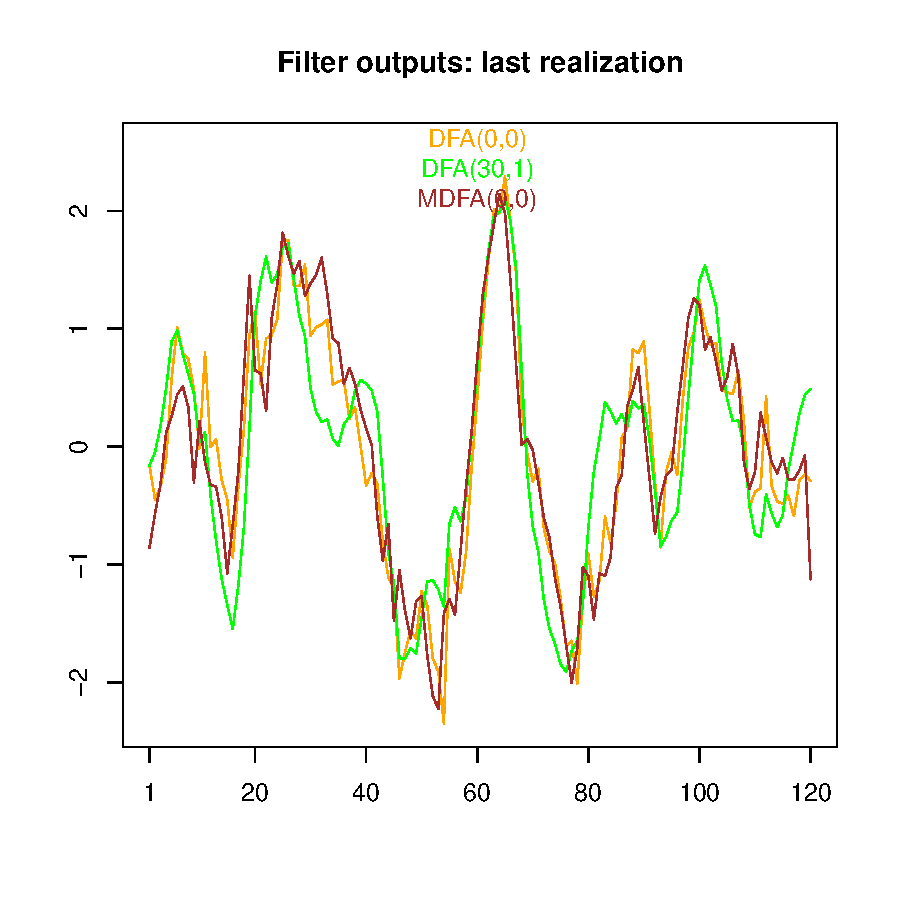
\includegraphics[height=4in, width=6in]{z_dfa_cust_mdfa_leading_indicator}\caption{Scaled outputs of DFA-MSE (orange), DFA-balanced (green) and bivariate MDFA-MSE (brown): a1=0.9\label{z_dfa_cust_mdfa_leading_indicator}}\end{center}\end{figure}The customized DFA (green) appears faster and smoother, as expected. Note that the leading-indicator design (brown) is systematically faster than DFA-MSE (orange) in the turning-points.  \\

We retain from the above example that a suitably customized \emph{univariate} design can outperform a classic MSE bivariate leading-indicator design, in-sample and out-of-sample, in terms of Peak Correlation and Curvature. A direct comparison of univariate and bivariate MSE-designs illustrates that the latter outperforms the former merely in terms of Peak Correlation (due to the leading indicator); gains in terms of MSE- or Curvature are moderate, at least out-of-sample.



\section{An Extended Customization Triplet}\label{customization_triplet}

Overemphasizing the Timeliness contribution to the MSE-norm, in the schematic criterion \ref{ats_cust} or in criterion \ref{dfatp}, provides a direct control of the magnitude of the time-shift of a real-time filter in the passband: as a result the filter-output shifts to the left, as confirmed by the Peak-Correlation statistic. As a possible alternative, the time-shift contribution to the MSE-norm can be overemphasized by targeting a lead $l>0$ of the signal 
\begin{equation}\label{forecast_targ_spe}
\exp(i l \omega)\Gamma(\omega)
\end{equation}
where $\Gamma(\omega)$ designates the original target. Note that $l$ corresponds to $-Lag$ in our R-code. In order to simplify the exposition we assume that $\Gamma(\omega)\geq 0$ is the transfer function of the ideal trend. Then 
\[
\Phi(\omega)=-Arg(\exp(i l \omega)\Gamma(\omega))=-l\omega
\]
and the mean-square error becomes
\begin{eqnarray}
MSE&=&\frac{2\pi}{ T} \sum_{\textrm{Passband}} (\Gamma(\omega_k)-\hat{A}(\omega_k))^2 I_{TX}(\omega_k)\nonumber\\
&&+\frac{2\pi}{ T} \sum_{\textrm{Stopband}} (\Gamma(\omega_k)-\hat{A}(\omega_k))^2 I_{TX}(\omega_k)\nonumber\\
&&+\frac{2\pi}{ T}  \sum_{\textrm{Passband}} 4\Gamma(\omega_k)\hat{A}(\omega_k)\sin\left(\frac{\hat{\Phi}(\omega_k)+l\omega_k}{2}\right)^2 I_{TX}(\omega_k) \label{once_more_timeliness}
\end{eqnarray}
where we used the fact that $\Gamma(\omega)=A(\omega)$ since the transfer function is positive everywhere.
Since our target is the ideal lowpass, we expect that $\hat{\Phi}(\omega_k)>0$ in the passband: the output is shifted to the right with respect to the target. Therefore 
\[
\sin\left(\frac{\hat{\Phi}(\omega_k)+l\omega_k}{2}\right)^2>\sin\left(\frac{\hat{\Phi}(\omega_k)}{2}\right)^2
\]
if $l>0$. As a result, the Timeliness term \ref{once_more_timeliness} inflates, in contrast to Accuracy and Smoothness, which remain unaffected by the lead-time. The resulting effect must be similar, though not identical, to a specific magnification of Timeliness in the ATS-trilemma and therefore we expect the output of the resulting \emph{forecast} filter ($Lag=-l<0$) to lie to the left of the corresponding nowcast filter ($Lag=0$).\\


Instead of interpreting the forecast lead as a possible (indirect) alternative for controlling Timeliness, in lieu of $\lambda$, say, we envisage a combination of $l$ and of the customization parameters: we consider the triplet $(l, \lambda, \eta)$ as a natural extension of the original customization pair $(\lambda,\eta)$. The additional `customization' parameter $l>0$ is helpful and effective if the time-shift of a particular real-time design is small already, in which case Timeliness cannot be substantially reduced anymore by selecting $\lambda>0$: a corresponding example is provided in section \ref{customization_cf} (customization of the Christiano Fitzgerald bandpass design). More generally and more formally, Timeliness is a measure of the phase error (the contribution of the phase to MSE)
\[
\frac{2\pi}{ T}  \sum_{\textrm{Passband}} 4A(\omega_k)\hat{A}(\omega_k)\sin\left(\frac{\hat{\Phi}(\omega_k)-\Phi(\omega_k)}{2}\right)^2
I_{TX}(\omega_k) 
\]
where $\Phi(\omega_k)=-l \omega_k$. Selecting $\lambda>0$, in criteria \ref{ats_cust} or \ref{dfatp}, shrinks the Timeliness term by pulling $\hat{\Phi}(\omega_k)$ towards $-l \omega_k$ or, equivalently, by attracting the time-shift $\hat{\phi}(\omega_k)=\hat{\Phi}(\omega_k)/\omega_k$ towards $-l$. In contrast to the original customization pair $(\lambda,\eta)$, the extended triplet $(l,\lambda,\eta)$ allows to design filters with more general lead or lag properties. A worked-out example is provided in chapter \ref{rep_sec}, section \ref{customization_cf}.





\section{Summary}

\begin{itemize}
\item The MSE-norm can be split into Accuracy, Timeliness and Smoothness components\footnote{The Residual either vanishes or is negligible in practice.}. 
\item The MSE-paradigm is replicated by weighting ATS-components equally. Equal-weighting reflects one particular `diffuse' research priority.
\item A strict MSE-approach is unable, per definition, to address Timeliness and Smoothness, either separately or all together.
\item The ATS-trilemma degenerates to a AT-dilemma in the case of classic (allpass) forecasting. Stated otherwise: classic (quasi maximum likelihood) forecast approaches have a blind spot. 
\item Curvature and  Peak-Correlation performances can be addressed simultaneously by customized designs. 
%\item In a growth-perspective -- data and signals in {first differences} -- suitably customized designs improve `mechanically'  MSE-performances at the important turning-points of a time series;  at costs of MSE-performances at all other time points, between consecutive turning-points. 
\item The DFA and the resulting ATS-trilemma are generic concepts: they allow for arbitrary target signals as well as arbitrary spectral estimates. Model-based targets and (pseudo) spectral densities are addressed in chapter \ref{rep_sec}.
\item The generic customization triplet $(l,\lambda,\eta)$ extends the action of the ATS-trilemma to arbitrary real-valued lead or lag specifications. 
\item The DFA/MDFA optimization criteria appear to be surprisingly robust against overfitting. Emphasizing Smoothness reinforces this statement.
\end{itemize}
%Paradoxon 1: (real-time) filters with enhanced speed and noise-suppression properties do not necessarily perform better in terms of MSE-performances, quite the contrary. Paradoxon 2: directional forecast properties are not always improved by emphasizing Smoothness and Timeliness in the ATS-trilemma. For this to happen, it requires a time series -- a process --  which supports directional inference.  


%-------------------------------------------



\chapter{ATS-Trilemma: the Multivariate Case}\label{atsm_sec}


In this chapter, the ATS-trilemma and the customized optimization principle are generalized to a multivariate MDFA-framework. Section \ref{ats_trilemma_and_cust} briefly reviews previously available criteria and derives all relevant concepts: multivariate ATS-trilemma, customized criterion, quadratic criterion and the corresponding closed-form solution; section \ref{mul_ats_tr_i_a} analyzes the effects obtained by emphasizing Timeliness and/or Smoothness in the new multivariate framework; finally, section \ref{emp_con_m_d} concludes by an empirical contest, comparing performances of univariate and multivariate MSE- and customized designs.




\section{MDFA: ATS-Trilemma and Customization}\label{ats_trilemma_and_cust}


We briefly list previous optimization criteria and we derive a generalization of the ATS-trilemma to the MDFA. A quadratic approximation of the estimation problem is proposed with a corresponding unique closed-form solution.  


\subsection{A Review of Previous Optimization Criteria}


\subsubsection{DFA-MSE}

\begin{eqnarray}
\frac{2\pi}{T}\sum_{k=-[T/2]}^{[T/2]}\left|\Gamma(\omega_k)-\hat{\Gamma}(\omega_k) \right|^2 I_{TX}(\omega_k)\to\min_{\mathbf{b}} \label{dfa_ms_e}
\end{eqnarray}
see \ref{dfa_ms}.



\subsubsection{MDFA-MSE}

\begin{equation}\label{dfanv_e}
\frac{2\pi}{T} \sum_{k=-T/2}^{T/2}
\left|\left(\Gamma(\omega_k)-\hat{\Gamma}_X(\omega_k)\right)\Xi_{T
X}(\omega_k)-\sum_{n=1}^m
\hat{\Gamma}_{W_n}(\omega_k)\Xi_{TW_n}(\omega_k)\right|^2 \to \min_{\mathbf{B}}
\end{equation}
see \ref{dfanv}. In matrix-notation we obtain

\begin{eqnarray}\label{regms_e}
(\mathbf{Y_{\textrm{rot}}-X_{\textrm{rot}}b})'(\mathbf{Y_{\textrm{rot}}-X_{\textrm{rot}}b})\to\min_{\mathbf{b}}
\end{eqnarray}
where $\mathbf{b}:=\textrm{Vec}(\mathbf{B})$ is the vector of stacked columns of $\mathbf{B}$. The solution is
\begin{eqnarray}\label{bregms_e}
\mathbf{\hat{b}}&=&\mathbf{\left(\Re(X_{\textrm{rot}}'X_{\textrm{rot}})\right)^{-1}\Re(X_{\textrm{rot}})'Y_{\textrm{rot}}}
\end{eqnarray}
see section \ref{gen_le_sq_sol}. The solution of the constrained optimization problem was proposed in \ref{const_sol}. 


\subsubsection{Customized DFA}

\begin{eqnarray}
&&\frac{2\pi}{ T} \sum_{\textrm{All~Frequencies}} (A(\omega_k)-\hat{A}(\omega_k))^2 W(\omega_k,\eta) I_{TX}(\omega_k)\nonumber\\
&&+(1+\lambda)\frac{2\pi}{ T}  \sum_{\textrm{Passband}} 4A(\omega_k)\hat{A}(\omega_k)\sin(\hat{\Phi}(\omega_k)/2)^2
I_{TX}(\omega_k)\to\min_{\mathbf{b}}\label{dfatp_e}
\end{eqnarray}
see \ref{dfatp}. The analytically tractable quadratic expression is
\begin{eqnarray}\label{idfa_s}
&&\frac{2\pi}{T} \sum_{k=-[T/2]}^{[T/2]}
 \left|\big|\Gamma(\omega_k)\Xi_{TX}(\omega_k)\big|-\left\{\Re\left[\hat{\Gamma}(\omega_k)\Xi_{TX}(\omega_k)\exp\big(-i\arg\big\{\Gamma(\omega_k)\Xi_{TX}(\omega_k)\big\}\big)\right]\right.\right.\nonumber\\
 &&\left.\left.+i\sqrt{1+\lambda|\Gamma(\omega_k)|}
 \Im\left[\hat{\Gamma}(\omega_k)\Xi_{TX}(\omega_k)\exp\big(-i\arg\left\{\Gamma(\omega_k)\Xi_{TX}(\omega_k)\right\}\big)\right]\right\}\right|^2 W(\omega_k,\eta)\to\min_{\mathbf{b}}\nonumber\\
\end{eqnarray}
see \ref{idfa}.



\subsection{ATS-Trilemma and Multivariate Customization}\label{ats_tr_mu_cu}


A generalization of the customized criterion \ref{dfatp_e} to the multivariate case can  be gleaned from the timely ordering of criteria, by applying a simple, but effective, notational trick to the MSE-criterion \ref{dfanv_e}:
\begin{eqnarray}
\label{dfavtp}
&&\frac{2\pi}{T} \sum_{k=-T/2}^{T/2}
\left|\Gamma(\omega_k)\Xi_{TX}(\omega_k)-\hat{\Gamma}_X(\omega_k)\Xi_{TX}(\omega_k)-\sum_{n=1}^m\hat{\Gamma}_{W_n}(\omega_k)\Xi_{TW_n}(\omega_k)\right|^2 \nonumber \\
&=&\frac{2\pi}{T} \sum_{k=-T/2}^{T/2}
\left|\Gamma(\omega_k)-\hat{\Gamma}_X(\omega_k)-\sum_{n=1}^m\hat{\Gamma}_{W_n}(\omega_k)\frac{\Xi_{TW_n}(\omega_k)}{\Xi_{TX}(\omega_k)}\right|^2 \left|\Xi_{TX}(\omega_k)\right|^2 \nonumber\\
&=&\frac{2\pi}{T} \sum_{k=-T/2}^{T/2}
\left|\Gamma(\omega_k)-\tilde{\Gamma}(\omega_k)\right|^2 I_{TX}(\omega_k)\label{dtp}
\end{eqnarray}
where
\begin{eqnarray}\label{dftp1}
\tilde{\Gamma}(\omega_k):=\hat{\Gamma}_X(\omega_k)+\sum_{n=1}^m\hat{\Gamma}_{W_n}(\omega_k)\frac{\Xi_{TW_n}(\omega_k)}{\Xi_{TX}(\omega_k)}
\end{eqnarray}
Literally, expression \ref{dtp} `looks' very much like \ref{dfa_ms_e} (up to the fact that the former involves multiple time series and a richly parametrized multivariate filter). Therefore, we could re-write the ATS-components in \ref{mse_dec_ats} as 
\begin{eqnarray}
\left.\begin{array}{ccc}
\textrm{A(ccuracy)}&:=&\frac{2\pi}{ T} \sum_{\textrm{Passband}} (A(\omega_k)-\tilde{A}(\omega_k))^2 I_{TX}(\omega_k)\\
\textrm{S(moothness)}&:=&\frac{2\pi}{ T} \sum_{\textrm{Stopband}} (A(\omega_k)-\tilde{A}(\omega_k))^2 I_{TX}(\omega_k)\\
\textrm{T(imeliness)}&:=&\frac{2\pi}{ T}  \sum_{\textrm{Passband}} 4A(\omega_k)\tilde{A}(\omega_k)\sin(\tilde{\Phi}(\omega_k)/2)^2
I_{TX}(\omega_k)                                     \\
\textrm{R(esidual)}&:=&\frac{2\pi}{ T}  \sum_{\textrm{Stopband}} 4A(\omega_k)\tilde{A}(\omega_k)\sin(\tilde{\Phi}(\omega_k)/2)^2
I_{TX}(\omega_k)
\end{array}\right\}\label{mse_dec_ats_e}
\end{eqnarray}
where $\tilde{A}(\omega_k)$ and $\tilde{\Phi}(\omega_k)$ are amplitude and phase functions of the aggregate transfer function $\tilde{\Gamma}(\omega_k)$ defined in \ref{dftp1}. The generalized ATS-Trilemma is obtained by splitting the MSE-norm into ATS-contributions (Residual is ignored)
\begin{eqnarray*}
\textrm{MSE}=\textrm{Accuracy}+ \textrm{Timeliness}+ \textrm{Smoothness}
\end{eqnarray*}
and a schematic (simplified) customized criterion is obtained by assigning weights to its constituents
\begin{equation}\label{ats_cust_e}
\textrm{MSE-Cust}(\lambda_1,\lambda_2)=\textrm{Accuracy}+(1+\lambda_1) \textrm{Timeliness}+(1+\lambda_2) \textrm{Smoothness}\to \min_{\mathbf{B}}
\end{equation}
where $\mathbf{B}$ is the matrix of filter coefficients. Using the weighting-functions introduced in section \ref{gen_cust_crit} the multivariate customized criterion becomes
\begin{eqnarray}
&&\frac{2\pi}{T} \sum_{k=-[T/2]}^{[T/2]}
|\Gamma(\omega_k)-\tilde{\Gamma}(\omega_k)|^2 W(\omega_k,\eta)I_{TX}(\omega_k)\nonumber\\
&&+4\lambda\frac{2\pi}{ T} \sum_{k=-T/2}^{T/2}
A(\omega_k)\tilde{A}(\omega_k)\sin(\tilde{\Phi}(\omega_k)/2)^2
W(\omega_k,\eta)I_{TX}(\omega_k)\to\min_{\mathbf{B}}\label{dfatp_i}
\end{eqnarray}
Instead of customizing all sub-filters individually, the proposed generalization of \ref{dfatp_e} addresses the aggregate multivariate filter  $\tilde{\Gamma}(\omega_k)$  `directly': a single customization pair $(\lambda,\eta)$ addresses Timeliness and Smoothness of the compound filter output.  






\subsection{Quadratic Criterion}


The univariate quadratic customized criterion \ref{idfa_s} can be rewritten in the multivariate case as
\begin{eqnarray}\label{imdfa_ep}
&&\frac{2\pi}{T} \sum_{k=-[T/2]}^{[T/2]}
 \left|\big|\Gamma(\omega_k)\Xi_{TX}(\omega_k)\big|-\left\{\Re\left[\tilde{\Gamma}(\omega_k)\Xi_{TX}(\omega_k)\exp\big(-i\arg\big\{\Gamma(\omega_k)\Xi_{TX}(\omega_k)\big\}\big)\right]\right.\right.\nonumber\\
 &&\left.\left.+i\sqrt{1+\lambda|\Gamma(\omega_k)|}
 \Im\left[\tilde{\Gamma}(\omega_k)\Xi_{TX}(\omega_k)\exp\big(-i\arg\left\{\Gamma(\omega_k)\Xi_{TX}(\omega_k)\right\}\big)\right]\right\}\right|^2 W(\omega_k,\eta)\to\min_{\mathbf{b}}\nonumber\\
\end{eqnarray}
where $\tilde{\Gamma}(\omega_k)$ is the aggregated multivariate filter \ref{dftp1}. This criterion can be solved in closed-form, see below. Moreover, $\lambda$ and $\eta$ address the relevant Timeliness -- speed -- and Smoothness -- noise suppression -- issues. Finally, all previous criteria are nested in \ref{imdfa_ep}. In order to derive a corresponding solution we explode the former expression into contributions by all subfilters: 
\begin{eqnarray}
&&\frac{2\pi}{T} \sum_{k=-[T/2]}^{[T/2]}
 \left|\big|\Gamma(\omega_k)\Xi_{TX}(\omega_k)\big|-\Bigg\{\Re\left[\tilde{\Gamma}(\omega_k)\Xi_{TX}(\omega_k)\exp\big(-i\arg\big\{\Gamma(\omega_k)\Xi_{TX}(\omega_k)\big\}\big)\right]\right.\nonumber\\
 &&\left.+i\sqrt{1+\lambda|\Gamma(\omega_k)|}
 \Im\left[\tilde{\Gamma}(\omega_k)\Xi_{TX}(\omega_k)\exp\big(-i\arg\left\{\Gamma(\omega_k)\Xi_{TX}(\omega_k)\right\}\big)\right]\Bigg\}\right|^2 W(\omega_k,\eta)\nonumber\\
&=&\frac{2\pi}{T} \sum_{k=-[T/2]}^{[T/2]}
 \left|\left|\Gamma(\omega_k)\Xi_{TX}(\omega_k)\right|-\Bigg\{\Re\left[\hat{\Gamma}_X(\omega_k)\Xi_{TX}(\omega_k)\exp\big(-i\arg\left\{\Gamma(\omega_k)\Xi_{TX}(\omega_k)\right\}\big)\right.\right.\nonumber\\
&&+\sum_{n=1}^m \left.\hat{\Gamma}_{W_n}(\omega_k)\Xi_{TW_n}(\omega_k)\exp\big(-i\arg\left\{\Gamma(\omega_k)\Xi_{TX}(\omega_k)\right\}\big)\right]\nonumber\\
&&+i\sqrt{1+ \lambda\Gamma(\omega_k)}
 \Im\left[\hat{\Gamma}_X(\omega_k)\Xi_{TX}(\omega_k)\exp\big(-i\arg\left\{\Gamma(\omega_k)\Xi_{TX}(\omega_k)\right\}\big)\right.\nonumber\\
&&\left.\left.+\sum_{n=1}^m\left.\hat{\Gamma}_{W_n}(\omega_k)\Xi_{TW_n}(\omega_k))\exp\big(-i\arg\left\{\Gamma(\omega_k)\Xi_{TX}(\omega_k)\right\}\big)\right]\right\}\right|^2 W(\omega_k,\eta)\nonumber\\
&&\to\min_{\mathbf{B}}\label{imdfa_e}
\end{eqnarray}
Being a quadratic function of filter coefficients, criterion \ref{imdfa_e} can be solved in closed-form, see below.
If $\lambda=0$ then \ref{imdfa_e} and \ref{dfatp_i} are identical; indeed both criteria coincide with the MSE-criterion \ref{dfanv_e}. For $\lambda>0$, \ref{imdfa_e} and \ref{dfatp_i} are not strictly identical, anymore. However, as shown in section \ref{ti_o_app_idfa}, the former (quadratic criterion) approximates the latter (customized criterion) tightly, even if $\lambda\geq 0$ is large\footnote{Because phase-differences between target and aggregate multivariate output  are small (linearization).}. 






\subsection{Least-Squares Customized Solution}\label{l-scsmdfa}

We now generalize the MSE-expressions \ref{desmatrot} and \ref{desmatrot_y} of design matrix and target to the proposed customization-framework. Define
\begin{eqnarray*}
\mathbf{X}_{k}^{\textrm{Cust}}(\lambda,\eta)&:=&\left\{\Re(\mathbf{X}_{k}(\lambda,\eta))+i\sqrt{1+ \lambda\Gamma(\omega_k)}\Im(\mathbf{X}_{k}(\lambda,\eta))\right\}\sqrt{W(\omega_k,\eta)}\\
\mathbf{Y}^{\textrm{Cust}}(\eta)&:=& \left(\begin{array}{c}\left|\Gamma(\omega_0)\Xi_{TX}(\omega_0)\right|\sqrt{W(\omega_0,\eta)}\\ 
\sqrt{2}|\Gamma(\omega_1)\Xi_{TX}(\omega_1)|\sqrt{W(\omega_1,\eta)}\\
\sqrt{2}|\Gamma(\omega_2)\Xi_{TX}(\omega_2)|\sqrt{W(\omega_2,\eta)}\\
.\\
\sqrt{2}|\Gamma(\omega_{T/2})\Xi_{TX}(\omega_{T/2})|\sqrt{W(\omega_{T/2},\eta)}
\end{array}\right)
\end{eqnarray*}
where the target $\mathbf{Y}^{\textrm{Cust}}(\eta)$ depends on $\eta$, through the weighting function $W(\omega_k,\eta)$, and where 
\begin{eqnarray*}
\mathbf{X}_{k}(\lambda,\eta)'&=&\sqrt{1+I_{k>0}}\exp\big(-i\arg\left\{\Gamma(\omega_k)\Xi_{TX}(\omega_k)\right\}\big)\cdot\nonumber\\
&&\textrm{Vec}_\textrm{row}\left(\begin{array}{ccccc} \Xi_{TX}(\omega_k)& \exp(-i\omega_k)\Xi_{TX}(\omega_k)&...& \exp(-i(L-1)\omega_k)\Xi_{TX}(\omega_k)\\
 \Xi_{TW_1}(\omega_k)& \exp(-i\omega_k)\Xi_{TW_1}(\omega_k)& ...& \exp(-i(L-1)\omega_k)\Xi_{TW_1}(\omega_k)\\
 \Xi_{TW_2}(\omega_k)& \exp(-i\omega_k)\Xi_{TW_2}(\omega_k)& ...& \exp(-i(L-1)\omega_k)\Xi_{TW_2}(\omega_k)\\
...&...&...&...\\
 \Xi_{TW_m}(\omega_k)& \exp(-i\omega_k)\Xi_{TW_m}(\omega_k&...& \exp(-i(L-1)\omega_k)\Xi_{TW_m}(\omega_k)\\
\end{array}\right)
\end{eqnarray*}
whereby $\textrm{Vec}_\textrm{row}$ appends rows of a matrix to build a single long row-vector of dimension $(m+1)L$, recall section \ref{matrix_notation}. Finally, define $\mathbf{X}^{\textrm{Cust}}(\lambda,\eta)$ to be the customized design matrix whose $k$-th row is $\mathbf{X}_{k}^{\textrm{Cust}}(\lambda,\eta)'$, as defined above. Since the target vector is already real and positive we can save the rotation in section \ref{matrix_notation} and criterion   \ref{imdfa_e} can be rewritten more conveniently as 
\begin{eqnarray}\label{regcust}
(\mathbf{Y^{\textrm{Cust}}(\eta)-\mathbf{X}^{\textrm{Cust}}(\lambda,\eta)b})'(\mathbf{Y^{\textrm{Cust}}(\eta)-\mathbf{X}^{\textrm{Cust}}(\lambda,\eta)b})\to\min_{\mathbf{b}}
\end{eqnarray}
where $\mathbf{b}:=\textrm{Vec}(\mathbf{B})$ is the vector of stacked columns of $\mathbf{B}$. Accordingly, the customized coefficient estimate is obtained as 
\begin{eqnarray}\label{bregcust}
\mathbf{\hat{b}}^{\textrm{Cust}}(\lambda,\eta)&=&\mathbf{\left(\Re\Bigg\{(\mathbf{X}^{\textrm{Cust}}(\lambda,\eta))' \mathbf{X}^{\textrm{Cust}}(\lambda,\eta)\Bigg\}\right)^{-1}\Re(\mathbf{X}^{\textrm{Cust}}(\lambda,\eta)})'
\mathbf{Y^{\textrm{Cust}}(\eta)}
\end{eqnarray}
see section \ref{gen_le_sq_sol}. In order to avoid unnecessary overloading of notations in subsequent chapters we drop the parameters $(\lambda,\eta)$ in all customized expressions; we retain the superscript `Cust' to distinguish the customized estimate from the `plain vanilla' MSE-estimate \ref{bregms}, in the case $\lambda=\eta=0$.  Formally, it is an easy matter to account for additional I(1)- ($i1=T$) and/or I(2)- constraints ($i2=T$) proposed in chapter \ref{con_sec}: just add the superscript $\textrm{Cust}$ to all terms in the solution \ref{const_sol} (with all accompanying modifications). The generic MDFA-function 
\begin{Schunk}
\begin{Sinput}
> head(mdfa_analytic)
\end{Sinput}
\begin{Soutput}
1 function (L, lambda, weight_func, Lag, Gamma, eta, cutoff, i1,             
2     i2, weight_constraint, lambda_cross, lambda_decay, lambda_smooth,      
3     lin_eta, shift_constraint, grand_mean, b0_H0, c_eta, weight_structure, 
4     white_noise, synchronicity, lag_mat, troikaner)                        
5 {                                                                          
6     lambda <- abs(lambda)                                                  
\end{Soutput}
\end{Schunk}
handles the general case (and more, to come) whereas the context-specific variants
\begin{Schunk}
\begin{Sinput}
> head(MDFA_cust)
\end{Sinput}
\begin{Soutput}
1 function (L, weight_func, Lag, Gamma, cutoff, lambda, eta)                  
2 {                                                                           
3     lin_eta <- F                                                            
4     weight_constraint <- rep(1/(ncol(weight_func) - 1), ncol(weight_func) - 
5         1)                                                                  
6     lambda_cross <- lambda_smooth <- 0                                      
\end{Soutput}
\end{Schunk}
\begin{Schunk}
\begin{Sinput}
> head(MDFA_cust_constraint)
\end{Sinput}
\begin{Soutput}
1 function (L, weight_func, Lag, Gamma, cutoff, lambda, eta, i1, 
2     i2, weight_constraint, shift_constraint)                   
3 {                                                              
4     lin_eta <- F                                               
5     lambda_cross <- lambda_smooth <- 0                         
6     lambda_decay <- c(0, 0)                                    
\end{Soutput}
\end{Schunk}
handle multivariate customization with or without constraints imposed. We now analyze performances of multivariate customized designs. 




\section{The Multivariate ATS-Trilemma in Action}\label{mul_ats_tr_i_a}


\subsection{Empirical Framework}

We rely on the bivariate leading indicator design proposed in section \ref{leading_ind}. Specifically, we analyze the second process, $a_1=0.1$, and we target an ideal trend with cutoff $\pi/6$ by filters of length $L=12$. This design slightly departs from the previous chapter, where we selected cutoff $\pi/12$ and length $L=24$, because we do not want overfitting to interfer with our results in the richer multivariate framework\footnote{Recall that a minimal filter-length of $L=2\pi/(\pi/6)=12$ is required in order to suppress frequency $\pi/6$, as required by the cutoff, and that $2*L=24$ filter coefficients are estimated for the bivariate filters in samples of length $T=120$ (which corresponds to ten years of monthly data).}. 





\subsection{Emphasizing Smoothness: $\eta\geq 0$, $\lambda=0$ Fixed}\label{e_s_mdfa}

We fix $\lambda=0$ and let $\eta_k=0.3*k, k=0,...,6$.

\subsubsection{Run the Code}


\begin{Schunk}
\begin{Sinput}
> # Second process
> a1<-0.1
> # Customization settings MDFA
> eta_mdfa<-0.3*(0:6)
> # Fix lambda=0
> lambda_mdfa<-rep(0,length(eta_mdfa))
> # Customization settings DFA
> lambda_vec<-lambda_vec
> eta_vec<-eta_vec
> # target
> cutoff<-pi/6
> # Filter length
> L<-12
> # Real-time design
> Lag<-0
> # No constraints
> i1<-i2<-F
> # Sample length 120
> len<-120
\end{Sinput}
\end{Schunk}
\begin{Schunk}
\begin{Sinput}
> cust_leading_obj<-mdfa_mse_leading_indicator_vs_dfa_customized(anzsim,a1,
+     cutoff,L,lambda_vec,eta_vec,len1,len,i1,i2,Lag,lambda_mdfa,eta_mdfa,troikaner)  
\end{Sinput}
\end{Schunk}
The above function generates artificial data, applies our general DFA ($dfa\textunderscore analytic$) and MDFA ($mdfa\textunderscore analytic$) estimation routines, computes amplitude and time-shift-functions, filter coefficients, ATS-components and filter-outputs as well as Peak Correlation and Curvature statistics.

\subsubsection{ATS-Components}

ATS-components of the aggregate filter, as defined in section \ref{ats_tr_mu_cu}, are calculated explicitly and returned by the multivariate MDFA-function
\begin{Schunk}
\begin{Sinput}
> tail(mdfa_analytic)
\end{Sinput}
\begin{Soutput}
186     else {                                                                      
187         return(list(b = b, trffkt = trffkt, rever = rever, Accuracy = Accuracy, 
188             Smoothness = Smoothness, Timeliness = Timeliness,                   
189             MS_error = MS_error))                                               
190     }                                                                           
191 }                                                                               
\end{Soutput}
\end{Schunk}
The results are summarized in table \ref{ats_comp_mdfa_S}.
% latex table generated in R 3.3.2 by xtable 1.8-2 package
% Fri Dec 16 15:22:12 2016
\begin{table}[ht]
\centering
\begin{tabular}{rrrrrr}
  \hline
 & Accuracy & Timeliness & Smoothness & Residual & MSE \\ 
  \hline
MDFA(0,0) & 0.020167 & 0.032431 & 0.052677 & 0.000000 & 0.105276 \\ 
  MDFA(0,0.3) & 0.032263 & 0.046041 & 0.034387 & 0.000000 & 0.112692 \\ 
  MDFA(0,0.6) & 0.049511 & 0.060152 & 0.022365 & 0.000000 & 0.132028 \\ 
  MDFA(0,0.9) & 0.071750 & 0.074737 & 0.013860 & 0.000000 & 0.160348 \\ 
  MDFA(0,1.2) & 0.097173 & 0.089669 & 0.007933 & 0.000000 & 0.194775 \\ 
  MDFA(0,1.5) & 0.123658 & 0.102905 & 0.004286 & 0.000000 & 0.230849 \\ 
  MDFA(0,1.8) & 0.151625 & 0.110037 & 0.002373 & 0.000000 & 0.264036 \\ 
   \hline
\end{tabular}
\caption{ATS-Components as a function of eta (lambda=0 fixed)} 
\label{ats_comp_mdfa_S}
\end{table}Smoothness decreases  monotonically as a function of $\eta$, as desired.



\subsubsection{Amplitude-Functions, Time-Shift Functions and Filter Coefficients}

The effect of the Smoothness-customization on amplitude- and time-shift functions of the subfilters, as well as on their coefficients, is visualized in fig.\ref{z_amp_shift_mdfacust_leadind_S}. Prior to interpreting these results let us emphasize that customization does not address the subfilters but the \emph{aggregate} filter $\tilde{\Gamma}(\cdot)$ defined in \ref{dftp1}. Therefore, the transformation of the sub-filters, analyzed here, is an `indirect' effect of customization.

\begin{figure}[H]\begin{center}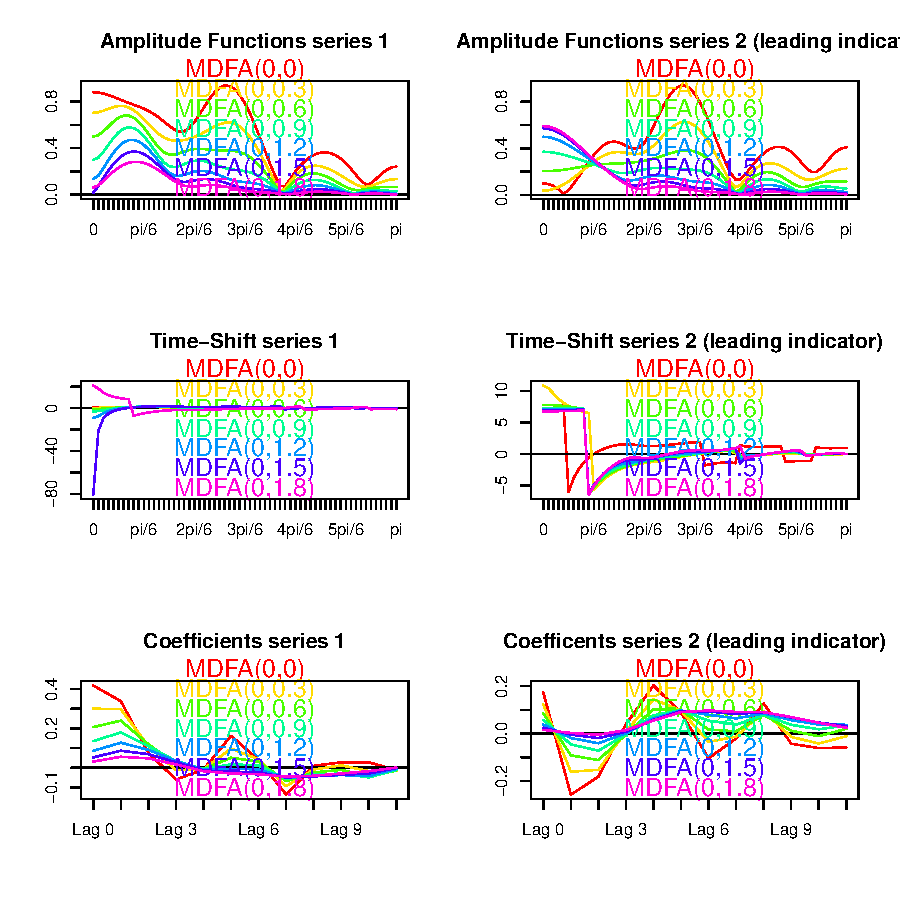
\includegraphics[height=8in, width=5in]{z_amp_shift_mdfacust_leadind_S}\caption{Amplitude (top), time-shift functions (middle) and filter coefficients (bottom): series 1 (left) and series 2 (right) for customized MDFA-leading indicator (emphasizing Smoothness): a1=0.1\label{z_amp_shift_mdfacust_leadind_S}}\end{center}\end{figure}\textbf{Analysis}
\begin{itemize}
\item Emphasizing Smoothness of the aggregate filter $\tilde{\Gamma}(\cdot)$, by $\eta$,  exerts effects on amplitude and time-shift functions of the subfilters $\hat{\Gamma}_X(\cdot), \hat{\Gamma}_{W_1}$ of the bivariate design which conform with expectations. In particular, the amplitude functions are shrinking in the stopband (stronger noise suppression) and the time-shifts are increasing in the passband, as $\eta$ increases\footnote{Note that the results obtained here are not directly comparable with those in section \ref{leading_ind} because the processes are different: $a_1=0.1$ (here) vs. $a_1=0.9$ (there).}.
\item As for the DFA in the previous chapter, emphasizing Smoothness, by $\eta$, seems to smooth filter coefficients too. This phenomenon, which is mainly due to the more or less intensive amplitude-shrinkage in the stop-band (steeper transfer function), implies that suitably customized filters are less prone to overfitting than classic MSE-designs. 
\end{itemize}



\subsubsection{Effects on Aggregated Filter}


Amplitude and time-shift functions of the aggregated filter $\tilde{\Gamma}(\cdot)$, defined in \ref{dftp1}, are plotted in fig. \ref{z_amp_shift_mdfacust_leadind_agg_S}.
\begin{figure}[H]\begin{center}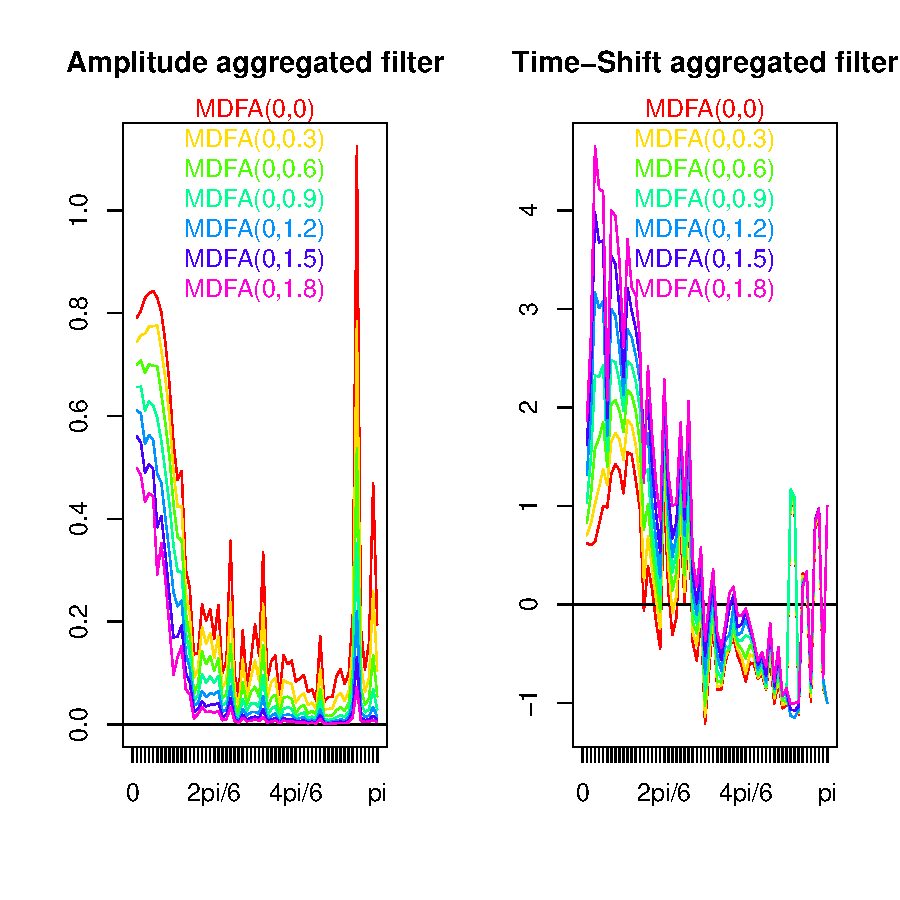
\includegraphics[height=3in, width=6in]{z_amp_shift_mdfacust_leadind_agg_S}\caption{Amplitude (left) and time-shift functions (right) of aggregated filter when emphasizing Smoothness: a1=0.1\label{z_amp_shift_mdfacust_leadind_agg_S}}\end{center}\end{figure}Note that the ratio of DFTs in \ref{dftp1} is uninformative in frequency zero and therefore we skipped the corresponding numbers. Both functions, amplitude and time-shift, are noisy because the DFT-ratio is noisy, too. Nevertheless, we can observe that the effect intended by $\eta$ is achieved by the aggregate: the amplitude function shrinks to zero in the stopband, as desired\footnote{The amplitude is also slightly shrunken in the passband, as expected, but shrinkage in the stopband is much stronger.} and the time-shift in the passband increases.







\subsection{Emphasizing Timeliness: $\lambda\geq 0$, $\eta=0$ Fixed}

We fix $\eta=0$ and let $\lambda_k=(0,2^k), k=0,...,7$.

\subsubsection{Run the Code}


\begin{Schunk}
\begin{Sinput}
> # Customization settings DFA
> lambda_mdfa<-c(0,2^(0:7))
> # Fix eta=0
> eta_mdfa<-rep(0,length(lambda_mdfa))
\end{Sinput}
\end{Schunk}
\begin{Schunk}
\begin{Sinput}
> cust_leading_obj<-mdfa_mse_leading_indicator_vs_dfa_customized(anzsim,a1,
+     cutoff,L,lambda_vec,eta_vec,len1,len,i1,i2,Lag,lambda_mdfa,eta_mdfa,troikaner)  
\end{Sinput}
\end{Schunk}



\subsubsection{ATS-Components}

ATS-components are summarized in table \ref{ats_comp_mdfa_T}.
% latex table generated in R 3.3.2 by xtable 1.8-2 package
% Fri Dec 16 15:22:12 2016
\begin{table}[ht]
\centering
\begin{tabular}{rrrrrr}
  \hline
 & Accuracy & Timeliness & Smoothness & Residual & MSE \\ 
  \hline
MDFA(0,0) & 0.020167 & 0.032431 & 0.052677 & 0.000000 & 0.105276 \\ 
  MDFA(1,0) & 0.031299 & 0.017587 & 0.060892 & 0.000000 & 0.109778 \\ 
  MDFA(2,0) & 0.038297 & 0.011085 & 0.066862 & 0.000000 & 0.116244 \\ 
  MDFA(4,0) & 0.046356 & 0.005646 & 0.074515 & 0.000000 & 0.126518 \\ 
  MDFA(8,0) & 0.053683 & 0.002395 & 0.082194 & 0.000000 & 0.138272 \\ 
  MDFA(16,0) & 0.059287 & 0.000931 & 0.088355 & 0.000000 & 0.148573 \\ 
  MDFA(32,0) & 0.063452 & 0.000364 & 0.092600 & 0.000000 & 0.156417 \\ 
  MDFA(64,0) & 0.066853 & 0.000148 & 0.095282 & 0.000000 & 0.162283 \\ 
  MDFA(128,0) & 0.069854 & 0.000063 & 0.096888 & 0.000000 & 0.166806 \\ 
   \hline
\end{tabular}
\caption{ATS-Components as a function of lambda (eta=0 fixed)} 
\label{ats_comp_mdfa_T}
\end{table}Timeliness decreases  monotonically as a function of $\lambda$, as required. We here skip the sub-filters and go straight to the interesting aggregate.




\subsubsection{Effects on Aggregated Filter}


Amplitude and time-shift functions of the aggregated filter $\tilde{\Gamma}(\cdot)$, defined in \ref{dftp1}, are plotted in fig. \ref{z_amp_shift_mdfacust_leadind_agg_T}.
\begin{figure}[H]\begin{center}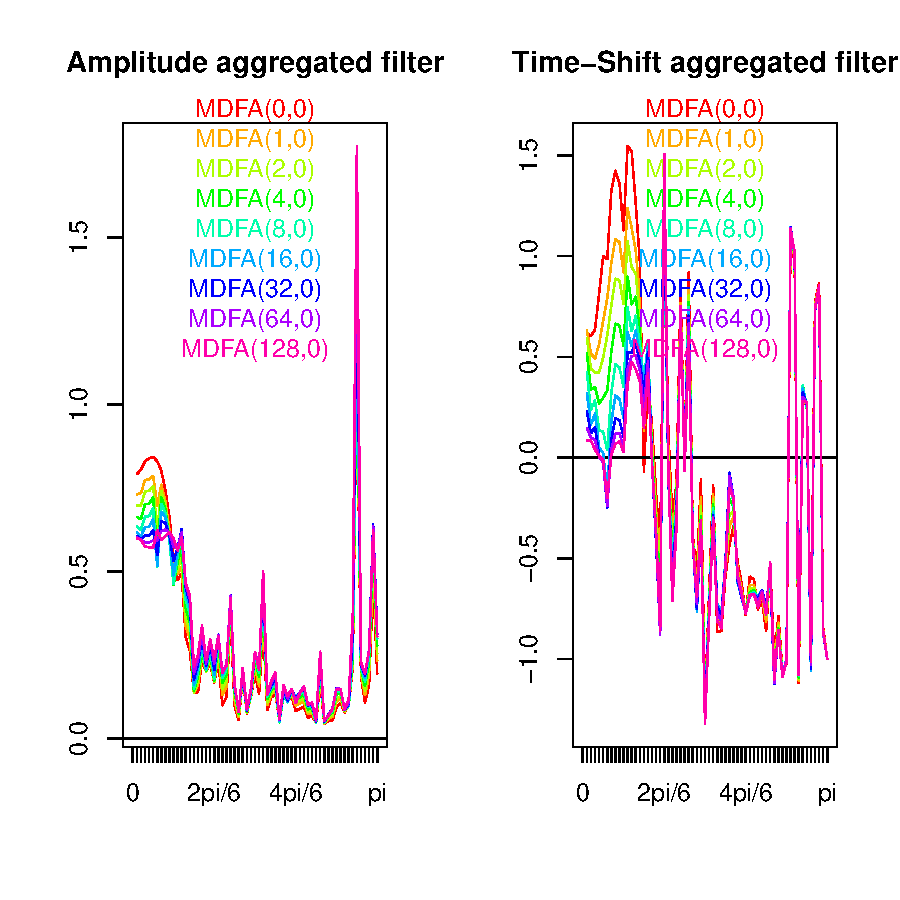
\includegraphics[height=3in, width=6in]{z_amp_shift_mdfacust_leadind_agg_T}\caption{Amplitude (left) and time-shift functions (right) of aggregated filter when emphasizing Timeliness: a1=0.1\label{z_amp_shift_mdfacust_leadind_agg_T}}\end{center}\end{figure}We can observe that the effect intended by emphasizing Timeliness is achieved: the time-shift of $\tilde{\Gamma}(\cdot)$ approaches zero in the passband as $\lambda$ increases.







\subsection{Emphasizing Timeliness and Smoothness: : $\lambda> 0$, $\eta>0$}

We compare MSE and balanced customized $\lambda=30,\eta=1$ designs: the latter refers to the univariate balanced DFA-design in section \ref{double_score_ats}.

\subsubsection{Run the Code}


\begin{Schunk}
\begin{Sinput}
> # Customization settings DFA
> lambda_mdfa<-c(0,30)
> # Fix eta=0
> eta_mdfa<-c(0,1)
\end{Sinput}
\end{Schunk}
\begin{Schunk}
\begin{Sinput}
> cust_leading_obj<-mdfa_mse_leading_indicator_vs_dfa_customized(anzsim,a1,
+     cutoff,L,lambda_vec,eta_vec,len1,len,i1,i2,Lag,lambda_mdfa,eta_mdfa,troikaner)  
\end{Sinput}
\end{Schunk}


\subsubsection{ATS-Components}

ATS-components are summarized in table \ref{ats_comp_mdfa_ST}.
% latex table generated in R 3.3.2 by xtable 1.8-2 package
% Fri Dec 16 15:22:13 2016
\begin{table}[ht]
\centering
\begin{tabular}{rrrrrr}
  \hline
 & Accuracy & Timeliness & Smoothness & Residual & MSE \\ 
  \hline
MDFA(0,0) & 0.020167 & 0.032431 & 0.052677 & 0.000000 & 0.105276 \\ 
  MDFA(30,1) & 0.262417 & 0.002423 & 0.008149 & 0.000000 & 0.272988 \\ 
   \hline
\end{tabular}
\caption{ATS-Components as a function of lambda and eta} 
\label{ats_comp_mdfa_ST}
\end{table}Timeliness and Smoothness decrease  with increasing $(\lambda,\eta)$-pair, as required. 




\subsubsection{Effects on Aggregated Filter}


Amplitude and time-shift functions of the aggregated filter $\tilde{\Gamma}(\cdot)$, defined in \ref{dftp1}, are plotted in fig. \ref{z_amp_shift_mdfacust_leadind_agg_ST}: note that we re-scaled the customized filter because of zero-shrinkage, recall section \ref{l_e_geq_0}.
\begin{figure}[H]\begin{center}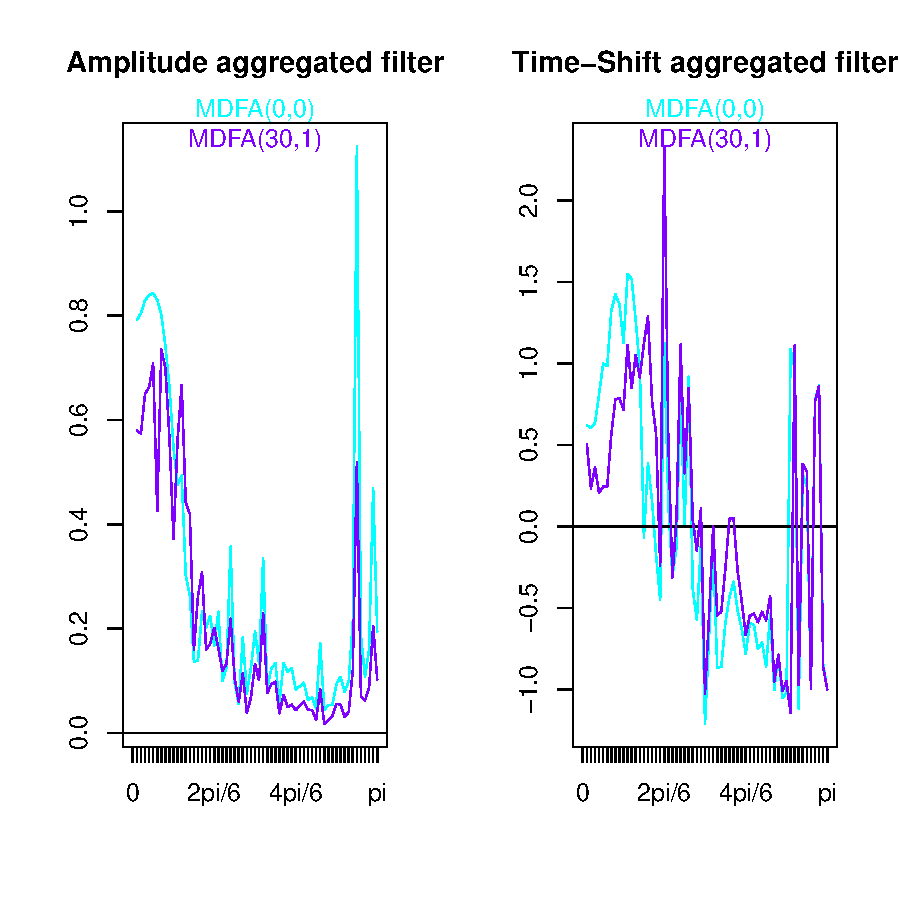
\includegraphics[height=3in, width=6in]{z_amp_shift_mdfacust_leadind_agg_ST}\caption{Amplitude (left) and time-shift functions (right) of aggregated filter when emphasizing Timeliness: a1=0.1\label{z_amp_shift_mdfacust_leadind_agg_ST}}\end{center}\end{figure}The effects intended by emphasizing Timeliness and Smoothness are achieved: the amplitude of the customized $\tilde{\Gamma}(\cdot)$ is closer to zero in the stopband and its time-shift is closer to zero in the passband. We now measure the relevant impact of customization on Curvature and Peak Correlation statistics.






\section{Empirical Contest: MDFA vs. DFA}\label{emp_con_m_d}

In contrast to the previous section we here address multiple realizations of the process and derive in-sample as well as out-of-sample distributions of Peak Correlation, Curvature and MSE performance measures. The empirical design is the same as in the previous section: we target an ideal trend with cutoff $\pi/6$, based on filters of length $L=12$. The contenders in our study are univariate (DFA) and bivariate (MDFA) \emph{MSE}-designs ($\lambda=\eta=0$) and  \emph{customized} DFA and MDFA `balanced' designs  $\lambda=30,\eta=1$: four competitors, one of each kind. 

\begin{Schunk}
\begin{Sinput}
> # Customization MDFA: MSE and balanced designs
> lambda_mdfa<-c(0,30)
> eta_mdfa<-c(0,1.)
> # Customization DFA: MSE and balanced designs
> lambda_vec<-c(0,30)
> eta_vec<-c(0,1)
> # Second process
> a1<-0.1
> # target
> cutoff<-pi/6
> # Filter length
> L<-12
> # Real-time design
> Lag<-0
> # No constraints
> i1<-i2<-F
> # Sample length 120
> len<-120
> # Number of replications
> anzsim<-100
\end{Sinput}
\end{Schunk}
\begin{Schunk}
\begin{Sinput}
> cust_leading_obj<-mdfa_mse_leading_indicator_vs_dfa_customized(anzsim,a1,
+     cutoff,L,lambda_vec,eta_vec,len1,len,i1,i2,Lag,lambda_mdfa,eta_mdfa,troikaner)  
\end{Sinput}
\end{Schunk}


Box-plots of in-sample and out-of-sample Curvature, Peak Correlation and MSE-scores are depicted in fig.\ref{z_curv_mdfacust_leadind_ST}.
\begin{figure}[H]\begin{center}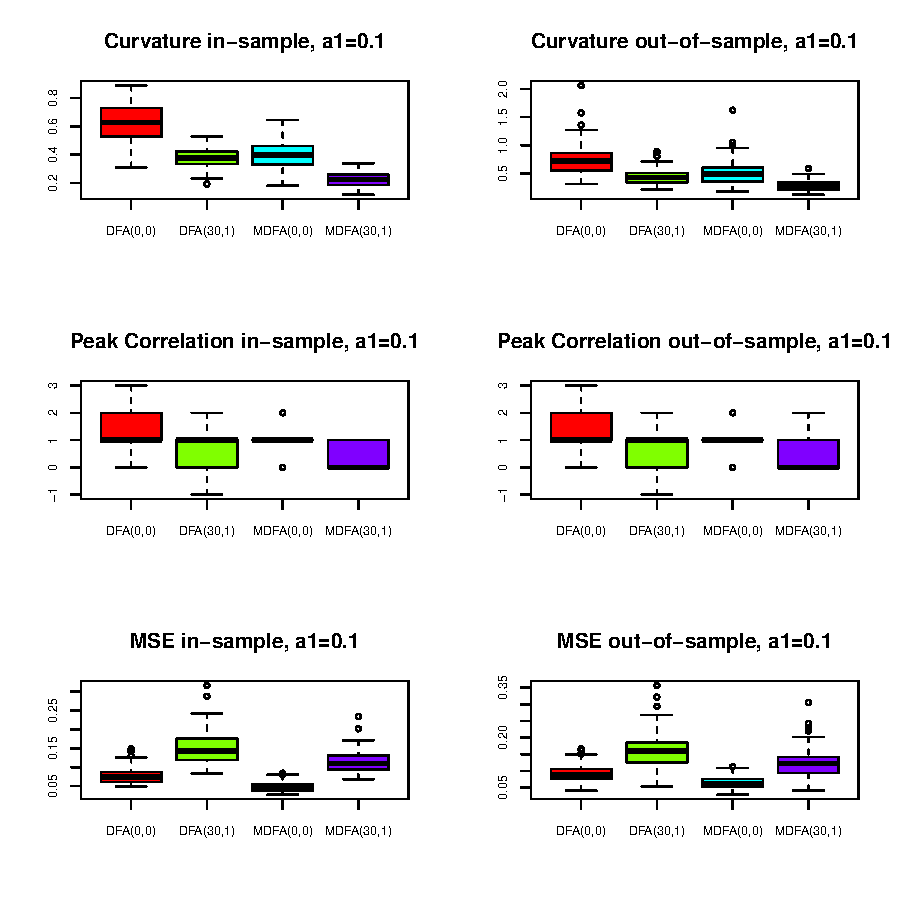
\includegraphics[height=7in, width=5in]{z_curv_mdfacust_leadind_ST}\caption{Curvature (top), Peak Correlation (middle) and MSE (bottom), in-sample (left) and out-of-sample (right) for MSE-DFA (red), balanced DFA (green), MSE-MDFA (cyan) and balanced MDFA (violet): a1=0.1\label{z_curv_mdfacust_leadind_ST}}\end{center}\end{figure}\textbf{Analysis}
\begin{itemize}
\item Recall that the empirical design is different than in section \ref{double_score_ats} so that performances cannot be compared directly. 
\item Both MSE-designs (red,cyan) are outperformed in terms of Curvature and Peak Correlation, by the balanced customized designs, in-sample and out-of-sample; but the latter loose in terms of MSE. 
\item The univariate balanced design (green) is outperformed by the multivariate balanced design (violet) on all accounts; in-sample as well as out-of-sample. Similarly, DFA-MSE (red) is outperformed by MDFA-MSE (cyan), in-sample and out-of-sample.
\item In-sample and out-of-sample performances are congruent which suggests that overfitting is avoided\footnote{The almost identical in- and out-of-sample distributions of Peak Correlation is due to discretization effects, since the Peak Correlation statistic is integer-valued.}.  
\end{itemize}




\section{Summary}

\begin{itemize}
\item The concepts in the previous chapter -- trilemma, customized criterion, quadratic criterion -- could be generalized to a multivariate framework by emphasizing the aggregate filter (output). Instead of tackling each sub-filter of the multivariate design separately, this proceeding addresses the problem in its entirety, by a single set of customization parameters $(\lambda,\eta)$.  
\item Empirical examples illustrate efficiency gains of MDFA vs. DFA in the context of the bivariate leading-indicator design. Multivariate designs (MSE/balanced customized) outperform their univariate siblings on all accounts: Timeliness, Curvature and MSE, in-sample as well as out-of-sample.
\item All previous optimization criteria are nested in the proposed multivariate closed-form solution.
\end{itemize}

%-------------------------------------------


\chapter{Replicating and Customizing Classic Model-Based Approaches}\label{rep_sec}

\section{Introduction}



The DFA is a generic signal extraction and forecast paradigm whose optimization criterion can be configurated by the user in order to align research priorities, problem structure and estimation principle. This chapter addresses the spectrum interface. In the generic DFA, the spectrum $h(\cdot)$ assigns a frequency-dependent weight to the approximation of $\Gamma(\cdot)$ by $\hat{\Gamma}(\cdot)$
\[\frac{2\pi}{T}\sum_{k=-[T/2]}^{[T/2]}\left|\Gamma(\omega_k)-\hat{\Gamma}(\omega_k) \right|^2 h(\omega_k)\]
If $h(\omega_k)$ is `large', in relative terms, then $\hat{\Gamma}(\omega_k) $ should match $\Gamma(\omega_k)$ closely in frequency $\omega_k$.
Interestingly, classic model-based ARIMA or state-space approaches  as well as classic filter designs, such as Hodrick Prescott, Christiano Fitzgerald or Henderson, for example, can be replicated up to arbitrary precision by specifying and inserting appropriate model-based or implied (pseudo-) spectral densities for $h(\omega_k)$ in the above expression. Once replicated, nothing stands in the way of customization: Timeliness and Smoothness or, equivalently, Peak Correlation and Curvature of classic time series approaches can be tackled at once.  A correspondingly customized model-based approach is a \emph{hybrid}: whereas the spectrum relies on (pseudo-) maximum likelihood, the filter output is obtained by emphasizing the filter error and by abandoning the mean-square perspective in the expanded scope of the ATS-trilemma. \\

Section \ref{rep_arima} emphasizes ARIMA-based approaches: an equivalence between (MSE-) DFA and model-based approaches (MBA) is established by linking time-domain and frequency-domain mean-square approaches; customization of the MBA by the DFA is discussed in section \ref{cust_mba_dfa_ar1}; section \ref{rep_cust_us_mod} addresses replication of unobserved components -- state space -- models whereby the DGP is factored into sub-processes (structural approach); section \ref{cust_uc_mod} handles customization of the latter; finally, section \ref{rep_cust_cl_fi_d} proposes replication and customization of classic filter designs, specifically HP and CF-filters.










\section{Replication of ARIMA-Based Approaches by the DFA}\label{rep_arima}

We show that forecast and signal-extraction performances of the classic ARIMA-based paradigm can be replicated by the DFA. 



\subsection{Framework}

In order to keep exposition simple and short we emphasize AR(1)-processes, our `fil rouge' introduced in section \ref{ex_dfa_1}. We assume that the DGP is known and we assume, also, that the target is an ideal trend with \emph{cutoff} $\pi/12$
\[\Gamma(\omega)=\left\{\begin{array}{cc}1~&~|\omega|\leq \pi/12\\0~&~\textrm{otherwise}\end{array}\right.\]
This is a typical target specification for monthly data in the context of business-cycle analysis.
The target is supposed to be approximated by \emph{real-time} designs: $Lag=0$. Note, however, that the scope of our analysis remains general: any ARIMA-process\footnote{Non-stationary integrated processes are analyzed in chapter \ref{int_sec}.} and/or any target signal\footnote{Model-based or non model-based (see further below); trend, cycle, seasonal adjustment or any combination thereof.} and/or any $Lag$ could be entertained by straightforward modifications. We now distinguish approaches according to whether (mean-square) solutions are obtained in the time domain or in the frequency domain.



\subsection{Time-domain}\label{time_domain}

The target signal 
\begin{equation}\label{target_ventimil}
y_t=\sum_{k=-\infty}^\infty\gamma_kx_{t-k}
\end{equation}
assumes knowledge of data $x_{t-k}, k<0$ that is unobserved at $t$, the time of inference. An optimal (mean-square) estimate $\hat{y}_T$ of $y_T$ in $t=T$ could be obtained by inserting optimal forecasts (and/or backcasts) of the unobservable data:
\begin{eqnarray*}
\hat{y}_T&=&\widehat{\sum_{k=-\infty}^{\infty}\gamma_kx_{T-k}}\\
&=&\sum_{k=-\infty}^{-1}\gamma_k\hat{x}_{T-k}+\sum_{k=0}^{T-1} \gamma_k{x}_{T-k}+\sum_{k=T}^{\infty}\gamma_k\hat{x}_{T-k}
\end{eqnarray*}
where $x_1,...,x_T$ is the observed data sample.
Inserting optimal forecasts and backcasts of the data, based on our AR(1)-specification, we obtain
\begin{eqnarray}
\hat{y}_T&=&\sum_{k=-\infty}^{-1}\gamma_k\hat{x}_{T-k}+\sum_{k=0}^{T-1} \gamma_k{x}_{T-k}+\sum_{k=T}^{\infty}\gamma_k\hat{x}_{T-k}\nonumber\\
&=&\sum_{k=-\infty}^{-1}\gamma_ka_1^{|k|}{x}_{T}+\sum_{k=0}^{T-1} \gamma_k{x}_{T-k}+\sum_{k=T}^{\infty}\gamma_k a_1^{k-(T-1)}{x}_1\label{backcasts}\\
&=&\left(\sum_{k=-\infty}^{0}\gamma_ka_1^{|k|}\right){x}_{T}+\sum_{k=1}^{T-2} \gamma_k{x}_{T-k}+\left(\sum_{k=T-1}^{\infty}\gamma_k a_1^{k-(T-1)}\right){x}_1\nonumber
\end{eqnarray}
We infer that the coefficients ${b}_j, j=0,...,T-1$ of the real-time filter $\hat{\Gamma}(\cdot)$ are obtained as
\begin{equation}\label{mba_coef_td}
{b}_j=\left\{\begin{array}{cc}\sum_{k=-\infty}^{0}\gamma_ka_1^{|k|}~,&~j=0\\\gamma_{j}~,&~j=1,...,T-2\\
\sum_{k=T-1}^{\infty}\gamma_k a_1^{k-(T-1)}~,&~j=T-1\end{array}\right.
\end{equation}
\textbf{Remarks}
\begin{itemize}
\item Frequently, backcasts can be neglected because the filter coefficients $\gamma_k$ decay sufficiently rapidly. For ease of exposition we now ignore the rightmost term in \ref{backcasts} (the simplification is mainly due to convenience and hence does not preclude generality). 
\item The proposed solution \ref{mba_coef_td} assumes $L=T$. Smaller $L$ are analyzed below. 
\end{itemize}
We briefly compute the resulting filter coefficients, which will then be replicated by the DFA. We use the three AR(1)-processes introduced in section \ref{ex_dfa_1}: $a_1=0.9,0.1,-0.9$:
\begin{Schunk}
\begin{Sinput}
> # Sample length
> len<-120
> # Specify lowpass target
> cutoff<-pi/12
> # Order of approximation of bi-infinite target by finite symmetric filter
> ord<-120
> # Compute coefficients gamma of symmetric filter
> gamma_k<-c(cutoff/pi,(1/pi)*sin(cutoff*1:ord)/(1:ord))
> # AR(1)-coefficient
> a_vec<-c(0.9,0.1,-0.9)
> # Initialize matrix of best MSE coefficients
> gamma_mba_rt<-matrix(ncol=length(a_vec),nrow=ord)
> for (k in 1:length(a_vec))
+ {
+ # Model-based filter: backcasts are ignored
+   gamma_0<-gamma_k%*%a_vec[k]^(0:ord)
+   gamma_mba_rt[,k]<-c(gamma_0,gamma_k[2:ord])
+ }
\end{Sinput}
\end{Schunk}




\subsection{Frequency-Domain}

An alternative solution of the mean-square filter approximation problem is obtained in the frequency domain
\[
\int_{-\pi}^\pi |\Gamma(\omega)-\hat{\Gamma}(\omega)|^2\frac{1}{|1-a_1\exp(-i\omega)|^2}d\omega\to \min_{\mathbf{b}}\]
where $\displaystyle{\frac{1}{|1-a_1\exp(-i\omega)|^2}}$ is the spectral density of the AR(1)-DGP.
The DFA MSE-criterion \ref{dfa_ms} stands for a particular empirical implementation of this theoretical criterion, whereby the continuous integral is replaced by a discrete sum and the periodogram is substituted for the true spectral density. In order to make the frequency-domain criterion operable we discretize the integral 
\begin{equation}\label{mba_rep_by_dfa}
\sum_{k=-M}^M|\Gamma(\omega_k)-\hat{\Gamma}(\omega_k)|^2\frac{1}{|1-a_1\exp(-i\omega_k)|^2}\to \min_{\mathbf{b}}
\end{equation}
where $\omega_k=k\pi/M,k=-M,...,M$, $M>0$ is a  discrete frequency-grid (the normalization constant can be omitted for optimization). The denseness of the frequency-grid, as specified by $M$, determines the tightness of the approximation of the exact solution by the discrete estimate\footnote{The quality of the approximation could be improved, to some extent, by allowing for a non-equidistant frequency-grid, modulating the density of the grid according to the steepness of the spectrum.}. In order to keep things simple we select $L=T=120$, as above, and $M=10*L=1200$. 

\begin{Schunk}
\begin{Sinput}
> # Frequency resolution: higher means tighter approximation 
> #   but computationally more intensive
> M<-10*len
> # Filter length
> L<-len
> # MSE-filter
> lambda<-0
> eta<-0
> # Real-time design
> Lag<-0
> # Unconstrained filter
> i1<-F
> i2<-F
> # Target in frequency-domain
> Gamma<-(0:M)<as.integer(cutoff*M/pi)+1
> omega_k<-(0:M)*pi/M
> # Coefficients of optimal MSE filter
> b_rt<-matrix(ncol=length(a_vec),nrow=ord)
> for (k in 1:length(a_vec))
+ {
+ # true spectral density
+   weight_func<-1/(abs(1-a_vec[k]*exp(1.i*omega_k))^2*2*pi)
+ # Estimate filter coefficients
+   dfa_ar1<-dfa_analytic(L,lambda,weight_func,Lag,Gamma,eta,cutoff,i1,i2)
+   b_rt[,k]<-dfa_ar1$b
+ }
> benchmark<-cbind(b_rt,gamma_mba_rt)
> dimnames(benchmark)[[2]]<-c(paste("MBA ",a_vec,sep=""),paste("DFA ",
+                                         a_vec,sep=""))
> dimnames(benchmark)[[1]]<-paste("lag ",0:(L-1),sep="")
\end{Sinput}
\end{Schunk}
We now briefly compare the previous time-domain (MBA) estimate to the latter frequency-domain (DFA) estimate:
\begin{Schunk}
\begin{Sinput}
> head(benchmark)
\end{Sinput}
\begin{Soutput}
         MBA 0.9    MBA 0.1   MBA -0.9    DFA 0.9    DFA 0.1   DFA -0.9
lag 0 0.42025712 0.09217342 0.04374995 0.42060902 0.09245016 0.04387223
lag 1 0.08217884 0.08218460 0.08218437 0.08238466 0.08238466 0.08238466
lag 2 0.07911787 0.07937846 0.07941692 0.07957747 0.07957747 0.07957747
lag 3 0.07492804 0.07493380 0.07493357 0.07502636 0.07502636 0.07502636
lag 4 0.06860857 0.06886916 0.06890762 0.06891611 0.06891611 0.06891611
lag 5 0.06158072 0.06158648 0.06158626 0.06149275 0.06149275 0.06149275
\end{Soutput}
\end{Schunk}
For each process, both estimates are close, as expected. The approximation could be tightened arbitrarily by selecting a denser frequency-grid (for the DFA) and by accounting for backcasts in the MBA. The DFA replicates the MBA, if the spectral density of the latter is used in the former. Since the process is assumed to be known, neither filter depends on data. In practice, a model must be identified and unknown parameters must be estimated. Of course, these intermediary steps do not affect the replication of the MBA by the DFA: just plug the estimated ARMA-parameters $\hat{b}_1,...,\hat{b}_{\hat{q}},\hat{a}_1,...,\hat{a}_{\hat{p}}$ of the former in the empirical spectral-density of the latter:
\[\hat{h}(\omega_k):=\left|\frac{1+\sum_{j=1}^{\hat{q}}\hat{b}_j\exp(-ij\omega_k)}{1-\sum_{j=1}^{\hat{p}}\hat{a}_j\exp(-ij\omega_k)}\right|^2\]
and plug the estimate into \ref{mba_rep_by_dfa}. An extension to integrated processes is provided in chapter \ref{int_sec}.



\subsection{Forecasting}

Since our target specification \ref{target_ventimil} is general, the forecast-problem is actually nested in the previous Signal-Extraction formalism: replace the (ideal trend) target by the anticipative $h-$steps ahead allpass filter
\[\Gamma_h(\omega)=\exp(ih\omega)~,~h>0\]
or, equivalently, set $\gamma_k=\left\{\begin{array}{cc}1~&,~k=-h\\0~&,~\textrm{otherwise}\end{array}\right.$
in  \ref{target_ventimil}.











\section{Customization of MBA by DFA: AR(1)-Process} \label{cust_mba_dfa_ar1}



\subsection{Known DGP} \label{true_dgp}



Having achieved replication of the MBA by the DFA, the next step addresses customization of the MBA by means of the replicating DFA. This natural extension allows to tackle Timeliness and Smoothness of (suitably customized) model-based designs. We first assume knowledge of the true DGP ($a_1$ is known). Our contenders are the classic MSE-filter $\lambda=\eta=0$, the balanced customized design $\lambda=30,\eta=1$, a strong smoothness filter $\lambda=0,\eta=1$ and a `fast-only' filter $\lambda=100,\eta=0$. The filter-length is fixed at $L=24$ and the denseness of the frequency-grid is preset at $M=T/2=60$\footnote{Our selection $L=24, M=60$ is a fairly good compromise ensuring statistical accuracy as well as computational speed. Note that $L=24$ is derived from the selected cutoff $\pi/12$: shorter filters would not be able to eliminate a component with frequency $\pi/12$. Note also that larger filter lengths $L$ might require denser frequency-grids (in order to avoid overfitting at the grid-points) which, in turn, would affect numerical speed.}.
\begin{Schunk}
\begin{Sinput}
> # Specify the processes: ar(1) with coefficients -0.9,0.1 and 0.9
> a_vec<-c(0.9,0.1,-0.9)
> # Specify the lambdas
> lambda_vec<-c(0,30,0,100)
> # Specify the fixed eta
> eta_vec<-c(0,1,1,0)
> # Length of model-based filters
> L<-24
> # Length of estimation sample (not used yet since we rely on the true model) 
> len<-120
> # Denseness frequency-grid
> M<-len/2
> # cutoff
> cutoff<-pi/12
> # Nowcast
> Lag<-0
> # No filter constraints
> i1<-i2<-F
> # Use model-based spectrum
> mba<-T
\end{Sinput}
\end{Schunk}
In the following simulation-run we generate 100 replications of the three AR(1)-processes and we use the true spectral densities i.e we do not estimate the AR(1)-parameter. We derive amplitude and time-shift functions, ATS-components, Peak Correlation and Curvature statistics as well as filter outputs.
\begin{Schunk}
\begin{Sinput}
> # Use true spectral density
> estim_MBA<-F
> anzsim<-100
> for_sim_obj<-for_sim_out(a_vec,len1,len,cutoff,L,mba,estim_MBA,L_sym,
+                 Lag,i1,i2,scaled_ATS,lambda_vec,eta_vec,anzsim,M,dif)
\end{Sinput}
\end{Schunk}
In order to save space we here emphasize the second process ($a_1=0.1$). Results for the other two processes are to be found in the appendix.
\begin{enumerate}
\item Amplitude and time-shift functions of the competing designs for the second process ($a_1=0.1$) are to be seen in fig.\ref{z_replication_amp_shift_dfa_2}. 
\begin{figure}[H]\begin{center}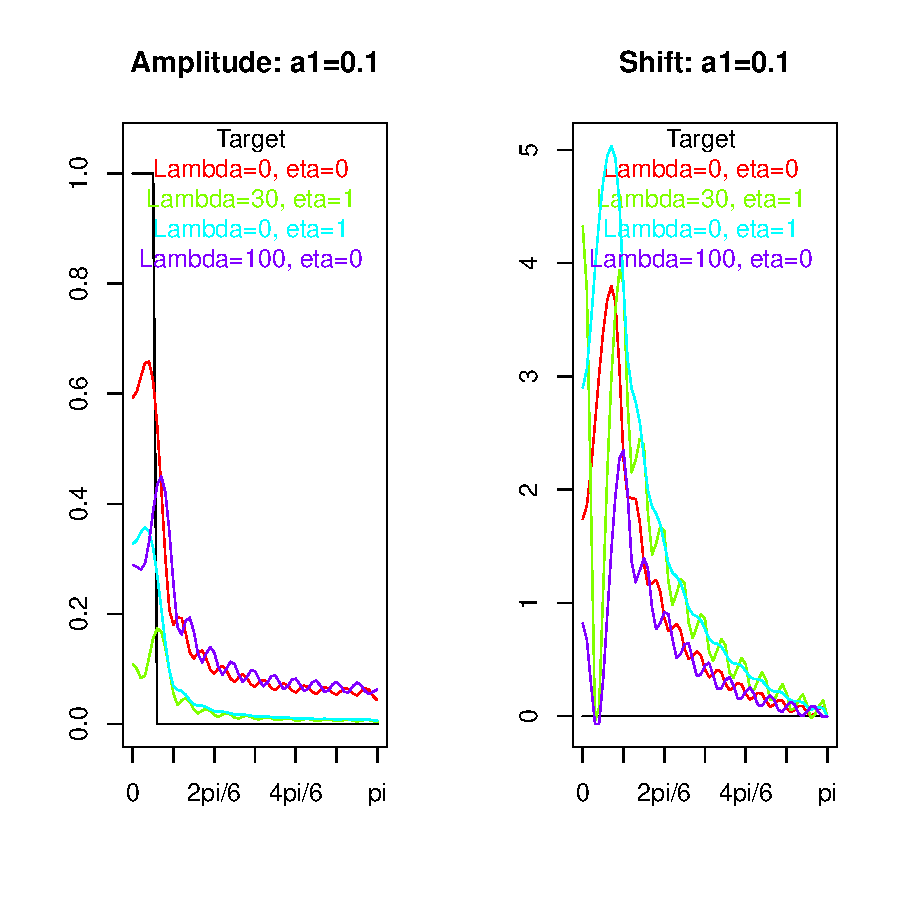
\includegraphics[height=4in, width=6in]{z_replication_amp_shift_dfa_2}\caption{Amplitude (left) and time-shift functions (right) of classic MSE model-based filter (red) vs. balanced model-based (green), smooth model-based (cyan) and fast model-based (violet);  a1=0.1\label{z_replication_amp_shift_dfa_2}}\end{center}\end{figure}\item The ATS-components of the competing designs, for the second process ($a_1=0.1$), are summarized in table \ref{z_replication_ats_dfa_2}.
% latex table generated in R 3.3.2 by xtable 1.8-2 package
% Fri Dec 16 15:24:06 2016
\begin{table}[ht]
\centering
\begin{tabular}{rrrrrr}
  \hline
 & Accuracy & Timeliness & Smoothness & Residual & Total MSE \\ 
  \hline
MBA-MSE & 0.017145 & 0.017543 & 0.019924 & 0.000000 & 0.054612 \\ 
  Lambda=30, eta=1 & 0.097701 & 0.000411 & 0.002061 & 0.000000 & 0.100173 \\ 
  Lambda=0, eta=1 & 0.053775 & 0.018166 & 0.003526 & 0.000000 & 0.075467 \\ 
  Lambda=100, eta=0 & 0.058692 & 0.000070 & 0.023573 & 0.000000 & 0.082335 \\ 
   \hline
\end{tabular}
\caption{ATS-Components: classic model-based vs. customized model-based } 
\label{z_replication_ats_dfa_2}
\end{table}
\item The empirical distributions of Curvature, Peak-Correlation and MSE are plotted in fig.\ref{z_replication_curv_peak_dfa_2}.

\begin{figure}[H]\begin{center}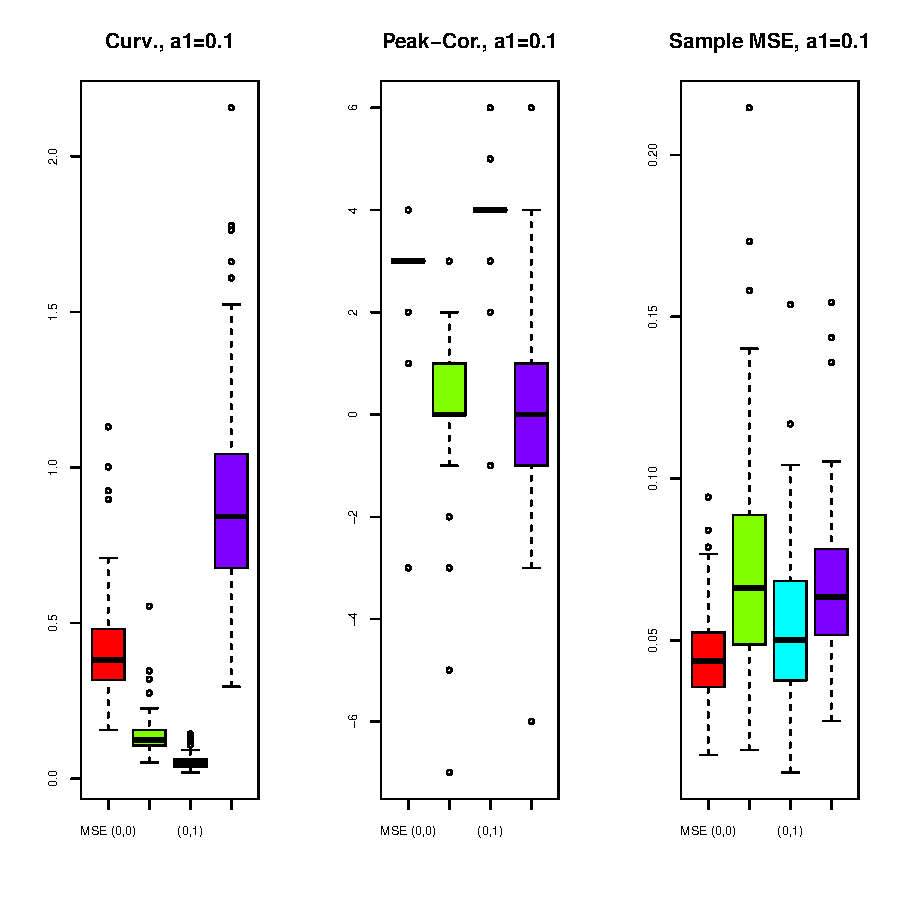
\includegraphics[height=4in, width=6in]{z_replication_curv_peak_dfa_2}\caption{Curvature (left), Peak Correlation (middle) and MSE distributions (right) of classic MSE model-based filter (red) vs. balanced model-based (green), smooth model-based (cyan) and fast model-based (violet);  a1=0.1\label{z_replication_curv_peak_dfa_2}}\end{center}\end{figure}\item A comparison of filter-outputs of classic model-based (red) and balanced model-based (green) is shown in fig.\ref{z_replication_output_dfa_2} (we selected the first realization of the process).
\begin{figure}[H]\begin{center}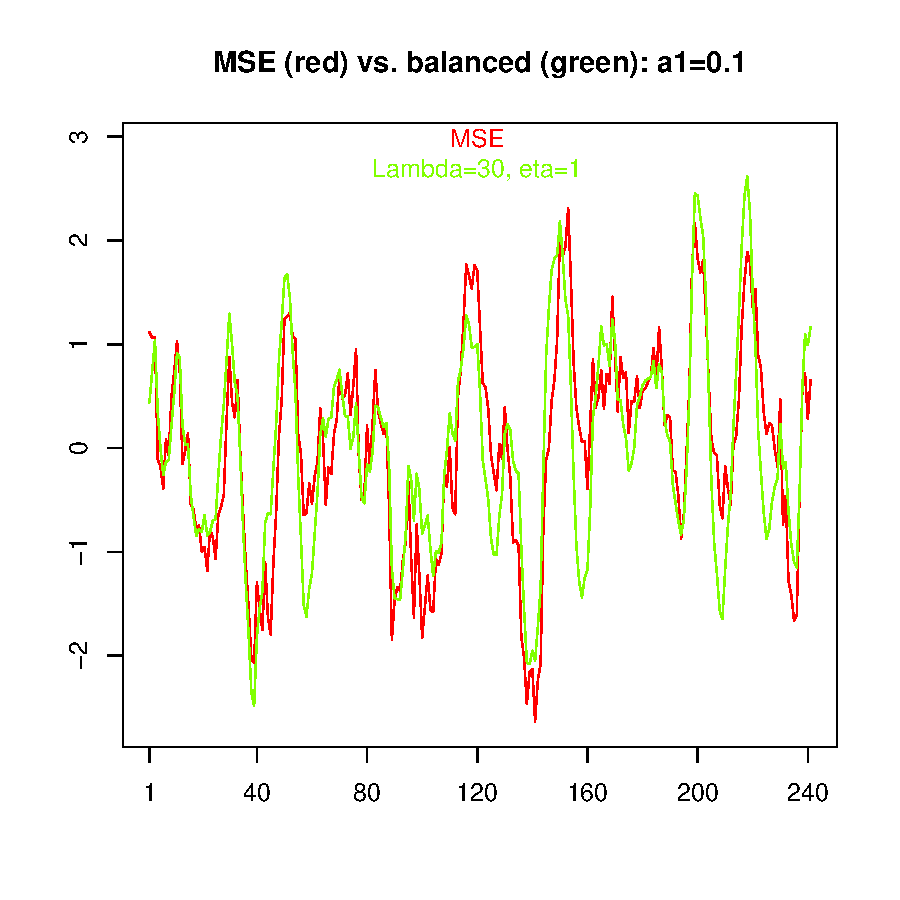
\includegraphics[height=4in, width=6in]{z_replication_output_dfa_2}\caption{Filter-outputs: classic MSE model-based filter (red) vs. balanced customized model-based (green);  a1=0.1\label{z_replication_output_dfa_2}}\end{center}\end{figure}\end{enumerate}
\textbf{Findings}
\begin{itemize}
\item The time-shifts in fig.\ref{z_replication_amp_shift_dfa_2} suggest that balanced (green) and fast (violet) filters should be faster than the classic MBA (red), even if the balanced filter has a larger shift in frequency zero\footnote{The spectral content in frequency zero does not dominate the dynamics of the second process (in contrast to a random-walk, for example).}; the smooth filter (cyan) is outperformed by the MBA. Amplitude functions are more difficult to interpret because of zero-shrinkage, recall section \ref{l_e_geq_0}. 
\item ATS-components in table \ref{z_replication_ats_dfa_2} behave as expected but interpretation is hampered by the fact that the statistics are not scale-invariant.
\item The scale-invariant Peak Correlation and Curvature statistics in fig.\ref{z_replication_curv_peak_dfa_2} reveal more effectively efficiency gains: the balanced model-based design (green) outperforms the classic MBA (red) on both accounts; but it is outperformed in terms of MSE-performances.
\item Finally, a comparison of filter outputs in fig.\ref{z_replication_output_dfa_2} (first realization of the process) confirms the previous picture: the customized design (green line) is smoother and it tends to anticipate turning points.
\end{itemize}








\subsection{Empirical AR(1)-Spectrum}\label{ar1_spect}


We assume that the true model-order -- AR(1) -- is known (no identification), but $a_1$ is unknown and must be estimated. The empirical spectral estimate is based on a fitted AR(1)-model and estimation relies on unconditional maximum likelihood, such as implemented in the R-function $arima$\footnote{Unconditional (full) maximum likelihood is obtained from a state-space model representation.}; estimates rely on samples of length $T=120$. In contrast to the previous section we here distinguish in-sample and out-of-sample performances of real-time (nowcast) filters.


\begin{Schunk}
\begin{Sinput}
> # Estimate the AR(1) coefficient
> estim_MBA<-T
> anzsim<-100
> for_sim_obj<-for_sim_out(a_vec,len1,len,cutoff,L,mba,estim_MBA,L_sym,
+               Lag,i1,i2,scaled_ATS,lambda_vec,eta_vec,anzsim,M,dif)
\end{Sinput}
\end{Schunk}
As in the previous section we emphasize the second process ($a_1=0.1$). In- and out-of-sample distributions of Peak Correlation and Curvature statistics are shown in fig.\ref{z_replication_curv_peak_dfa_2_emp}; corresponding MSE-distributions are to be found in fig.\ref{z_replication_curv_peak_dfa_2_emp_mse}.


\begin{figure}[H]\begin{center}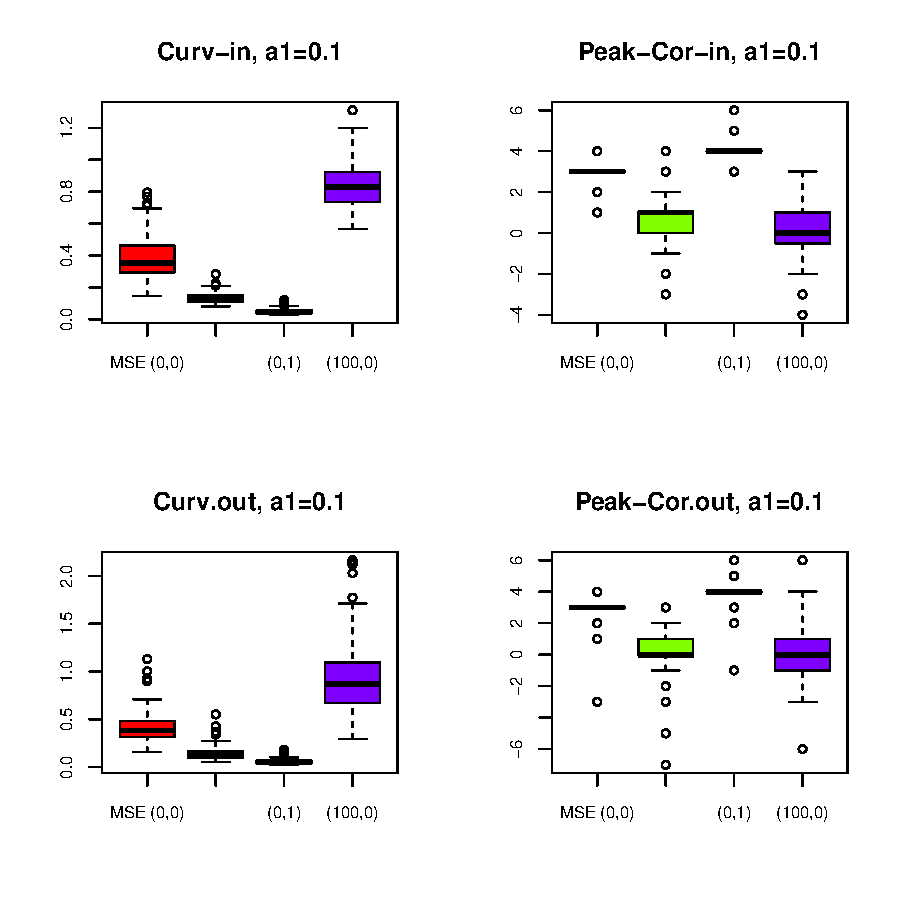
\includegraphics[height=6in, width=6in]{z_replication_curv_peak_dfa_2_emp}\caption{Curvature (left) and Peak Correlation (right) in-sample (top) and out-of-sample (bottom): classic MSE model-based filter (red) vs. balanced model-based (green), smooth model-based (cyan) and fast model-based (violet);  a1=0.1\label{z_replication_curv_peak_dfa_2_emp}}\end{center}\end{figure}
\begin{figure}[H]\begin{center}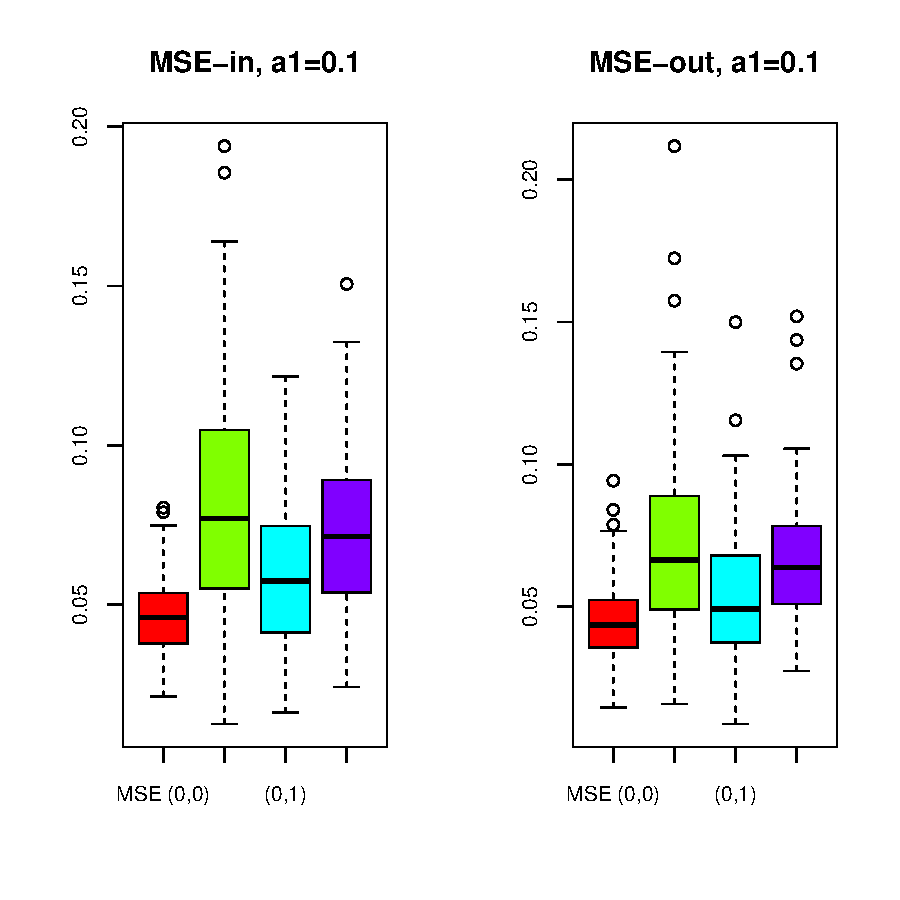
\includegraphics[height=4in, width=6in]{z_replication_curv_peak_dfa_2_emp_mse}\caption{MSE in-sample and out-of-sample: classic MSE model-based filter (red) vs. balanced model-based (green), smooth model-based (cyan) and fast model-based (violet);  a1=0.1\label{z_replication_curv_peak_dfa_2_emp_mse}}\end{center}\end{figure}
\textbf{Findings}
\begin{itemize}
\item The above results confirm our previous analysis: the balanced model-based design (green) outperforms the MBA in-sample as well as out-of-sample in terms of Curvature and Peak Correlation. The MBA performs best in terms of MSE, as expected.
\end{itemize}




\section{Replication of Unobserved-Components (UC-) Models}\label{rep_cust_us_mod}

In contrast to ARIMA-models, which model the entire DGP by a single (reduced-form) equation, an unobserved-components (UC-) model disaggregates the DGP into interesting `components', typically trend $T_t$, cycle $C_t$, seasonality $S_t$ and irregular $I_t$
\[x_t=T_t+C_t+S_t+I_t\]
Specific sub-models are assigned to the components which could be linked (dependency) or not (orthogonality) and the DGP of the data is obtained by aggregation of the components (structural form). We here review classic trend-cycle models for seasonally-adjusted log-transformed real US-GDP. 



\subsection{The Data: (Log) Real US GDP}

US (log) real GDP is plotted in fig.\ref{z_us_real_log_gdp}: the shaded areas correspond to recessions as declared by the NBER. The data is downloaded from the \href{https://www.quandl.com}{Quandl}-website, as illustrated in the following piece of code:
\begin{Schunk}
\begin{Sinput}
> # Post WWII data
> start_year<-1947 
> start_date=paste(start_year,"-01-01",sep="")
> # Last data point
> end_date<-format(Sys.time(), "%Y-%m-%d")
> end_year<-as.double(substr(end_date,1,4))
> # Load Real GDP
> #Title:               Real Gross Domestic Product, 3 Decimal
> #Series ID:           GDPC96
> #Source:              US. Bureau of Economic Analysis
> #Release:             Gross Domestic Product
> #Seasonal Adjustment: Seasonally Adjusted Annual Rate
> #Frequency:           Quarterly
> #Units:               Billions of Chained 2009 Dollars
> #Date Range:          1947-01-01 to 2014-07-01
> #Last Updated:        2014-11-25 7:56 AM CST
> #Notes:               A Guide to the National Income and 
> #                     Product Accounts of the United States 
> #                     (NIPA) - 
> #   (http://www.bea.gov/national/pdf/nipaguid.pdf)
> if (load_from_quandl)
+ {
+   mydata<-Quandl(c("FRED/GDPC96"),start_date=start_date,
+                end_date=end_date,type="xts")
+   save(mydata,file=paste(path.dat,"US_GDP.Rdata",sep=""))
+ } else
+ {
+   load(file=paste(path.dat,"US_GDP.Rdata",sep=""))
+ }
> tail(mydata)
\end{Sinput}
\begin{Soutput}
            [,1]
2015 Q2 16374.18
2015 Q3 16454.88
2015 Q4 16490.68
2016 Q1 16524.99
2016 Q2 16583.15
2016 Q3 16712.53
\end{Soutput}
\begin{Sinput}
> lgdp <- ts(100*log(mydata),start=start_year,frequency=4)
> nobs <- length(lgdp)
> # Annualized sharpe of GDP series
> sharpe_GDP<-sqrt(4)*mean(diff(lgdp))/sqrt(var(diff(lgdp)))
\end{Sinput}
\end{Schunk}
\begin{figure}[H]\begin{center}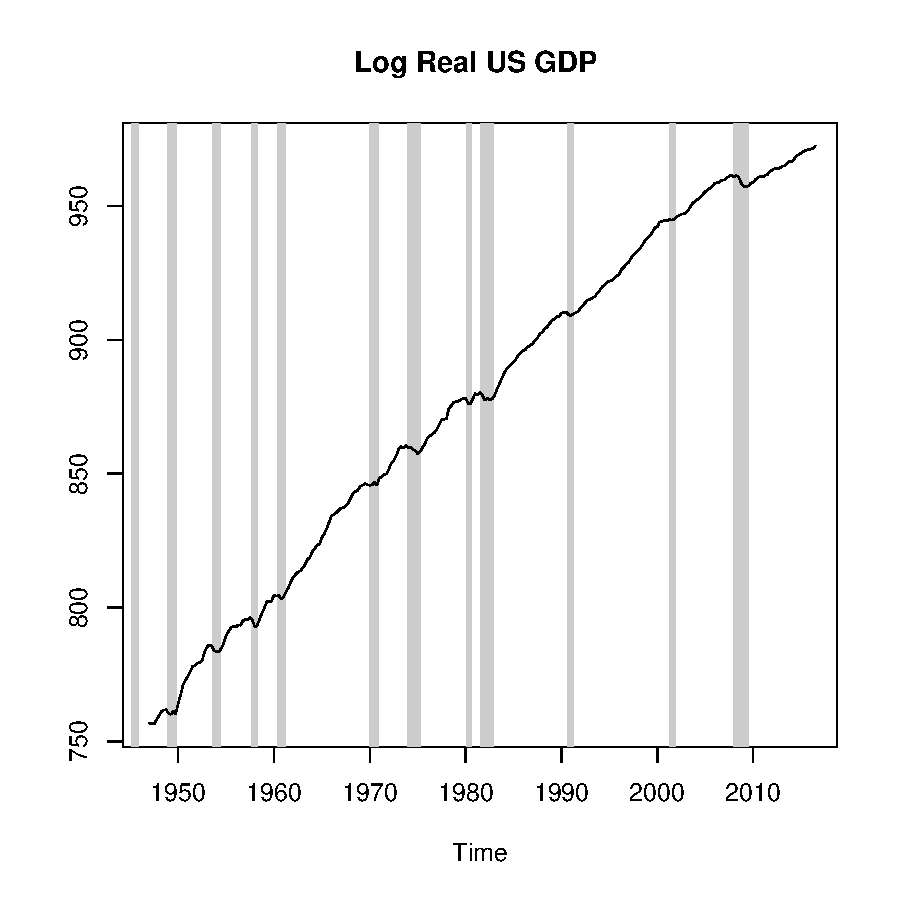
\includegraphics[height=4in, width=6in]{z_us_real_log_gdp}\caption{Log US Real GDP\label{z_us_real_log_gdp}}\end{center}\end{figure}Except for the (shaded) recession episodes, the series grows steadily: post-WWII annualized sharpe ratio is 1.64 and the drift is  regular but slightly decreasing towards the sample end. 


\subsection{UC-Model}

In order to fit the data,  Morley, Nelson, and Zivot (2003), \href{https://www.dropbox.com/s/1qn5h7s02c86j8i/mnz03.pdf?dl=0}{MNZ (2003)}, for short, propose the following Unobserved-Components (UC-) model
\begin{eqnarray}
\left.\begin{array}{ccc}
GDP_t&=&(1,1,0)\cdot\mathbf{S}_t+{v}_t\\
\mathbf{S}_t&=&\left(\begin{array}{c}\mu\\0\\0\end{array}\right)+\left(\begin{array}{ccc}1&0&0\\                           
                            0&a_1&1\\
                            0&a_2&0
                            \end{array}\right)\mathbf{S}_{t-1}+\mathbf{w_t}\end{array}\right\}\label{ss_mod_gen_i1}
\end{eqnarray}
where $v_t$ and $\mathbf{w}_t'=(w_{1t},w_{2t},0)$ are mutually uncorrelated iid random variables with variances $\sigma_v^2$, $\boldsymbol{\Sigma_w}^2=\left(\begin{array}{ccc}\sigma_{w,11}^2&0&0\\0&\sigma_{w,22}^2&0\\0&0&0\end{array}\right)$ and where $\mu$ is a constant drift. $\mathbf{S}_t$ collects trend (first component) and cycle (second component). If $\sigma_v^2=0$, as in \href{https://www.dropbox.com/s/1qn5h7s02c86j8i/mnz03.pdf?dl=0}{MNZ (2003)}, then  the data can be modeled by the sum of a random-walk with drift (trend) and a stationary AR(2) (cycle) whereby both processes are mutually independent. Given that the drift looses momentun after the dot-com recession (2001)\footnote{\href{https://www.dropbox.com/s/1qn5h7s02c86j8i/mnz03.pdf?dl=0}{MNZ (2003)} use data up to 1998.},  we complement the above fixed trend-growth model by an additional stochastic drift-equation in the system of state-equations:
\begin{eqnarray}
\left.\begin{array}{ccc}GDP_t&=&(1,0,1,0)\cdot\mathbf{S}_t+v_t\\
\mathbf{S}_t&=&\left(\begin{array}{cccc}1&1&0&0\\
                            0&1&0&0\\
                            0&0&a_1&1\\
                            0&0&a_2&0
                            \end{array}\right)\mathbf{S}_{t-1}+\mathbf{w_t}\end{array}\right\}\label{ss_mod_gen_i2}
\end{eqnarray}
where $\mathbf{w}_t'=(w_{1t},w_{2t},w_{3t},0)$ and $\boldsymbol{\Sigma_w}^2=\left(\begin{array}{cccc}\sigma_{w,11}^2&0&0&0\\0&\sigma_{w,22}^2&0&0\\0&0&\sigma_{w,33}^2&0\\0&0&0&0\end{array}\right)$. The first model is nested in this more general specification: set the second diagonal element $\sigma_{w,22}^2$ of $\boldsymbol{\Sigma_w}^2$,  corresponding to the adaptive drift, to zero and initialize the second element of $\mathbf{S}_0$ (drift) in $t=0$ by $\mu$. Note that if $\sigma_{w,22}^2>0$, then the DGP is integrated of order two (double unit root in frequency zero). Let  $\boldsymbol{\theta}'=(a_1,a_2,\sigma_{w,11}^2,\sigma_{w,22}^2,\sigma_{w,33}^2)$ designate the vector of unknown parameters. The latter can be estimated by maximizing the likelihood function, assuming that the noise terms are all Gaussian and mutually uncorrelated. 





\subsection{I(1)-Model MNZ (2003)}\label{mnz_m-gr}

We here rely on the R-package $dlm$
\begin{Schunk}
\begin{Sinput}
> library(dlm)
\end{Sinput}
\end{Schunk}
and fit model \ref{ss_mod_gen_i1}\footnote{More precisely, we fit \ref{ss_mod_gen_i2} with nesting constraints.} to the GDP data, assuming three different time spans: 
\begin{itemize}
\item Jan-1947 to Feb-1998: replicate results in \href{https://www.dropbox.com/s/1qn5h7s02c86j8i/mnz03.pdf?dl=0}{MNZ (2003)}
\item Jan-1947 to Dec-2007: validate the model on data prior to the great recession
\item Jan-1947 to Dec-2014: evaluate impact of great recession on model parameters. 
\end{itemize}
Let us emphasize that the Kalman-filter equations are (heavily) non-linear in the unknown variance parameters and therefore numerical optimization is challenging. The variances are crucial for determining the long-term dynamics (the integration order) of the DGP: if $\sigma_{w,22}^2=\sigma_{w,11}^2=0$ then the process is stationary (assuming stationarity of the cycle-AR(2)); if $\sigma_{w,22}^2=0$ and $\sigma_{w,11}^2>0$ then the process is integrated of order one I(1); if $\sigma_{w,22}^2>0$ then the process is integrated of order two I(2). 


\subsubsection{Data: Jan-1947 to Feb-1998}

In order to illustrate handling of the $dlm$-package we attempt to replicate results in \href{https://www.dropbox.com/s/1qn5h7s02c86j8i/mnz03.pdf?dl=0}{MNZ (2003)}. 

\begin{enumerate}
\item Data:
\begin{Schunk}
\begin{Sinput}
> # Post WWII data
> start_year<-1947 
> start_date=paste(start_year,"-01-01",sep="")
> # Data up to Feb-1998 as 
> end_date<-"1998-02-01"
> end_year<-as.double(substr(end_date,1,4))
> # Select data prior to end_year
> data_sample<-mydata[paste("/",end_date,sep="")]
> lgdp <- ts(100*log(data_sample),start=start_year,frequency=4)
> nobs <- length(lgdp)
\end{Sinput}
\end{Schunk}
\item Estimation: we replicate \ref{ss_mod_gen_i1} by \ref{ss_mod_gen_i2}, imposing $\sigma_{w,22}^2=0$. We refer the reader to the $dlm$-\href{http://cran.r-project.org/web/packages/dlm/vignettes/dlm.pdf}{vignette} for details of model implementation\footnote{We adapted code from \href{https://www.ualberta.ca/~sfossati/e509/files/slides/lec5.r}{Fossati (2013)}. In particular we parametrized the model in such a way that variances are always positive. Additionally, we can pre-specify and impose the argument of the roots of the AR(2) polynomial. This parameter is frequently (but erroneously) identified with the cycle-frequency, see section \ref{cf_cr_a_e_cl} for details.}. In order to exclude numerical issues, we used the solution in \href{https://www.dropbox.com/s/1qn5h7s02c86j8i/mnz03.pdf?dl=0}{MNZ (2003)} as initial value for our own optimization.
\begin{Schunk}
\begin{Sinput}
> # We specify the model: sigma_{w,22} is vanishing and sigma_v=sqrt(1e-7) 
> #   is nearly vanishing (slightly positive is needed for numerical 
> #   stability because otherwise 
> #   quotients can vanish in the Kalman-Filter).
> # Note also that all variances are parametrized as positive 
> #   constants (squares).
> # This parametrization replicates the model in MNZ (2003).
> ssm2 <- function(parm){
+   dlm <- dlmModPoly(2,dV=1e-7,dW=c(parm[4]^2,0)) + 
+     dlmModARMA(ar=c(parm[1],parm[2]), ma=NULL, sigma2=parm[3]^2)
+ 	# get distribution variance of initial state
+ 	tmp0 <- matrix(c(parm[1],parm[2],1,0),nr=2)
+ 	tmp1 <- matrix(c(parm[3]^2,0,0,0),nc=1)
+ 	tmp <- solve(diag(4)-tmp0%x%tmp0)%*%tmp1
+ 	dlm$C0[3:4,3:4] <- matrix(tmp,nr=2)
+ 	return( dlm )
+ }
> # Estimate parameters: we use the estimates in 
> #   Morley, Nelson and Zivot (2003) 
> # for initialization
> fit2_98 <- dlmMLE(y=lgdp,parm=c(1.5303,-.6097,.6199,.6893),build=ssm2,
+                   hessian=T)
\end{Sinput}
\end{Schunk}
The optimization affected slightly our initial estimates and therefore the final estimates in table \ref{z_ss_uc0_t} do not coincide with those reported in \href{https://www.dropbox.com/s/1qn5h7s02c86j8i/mnz03.pdf?dl=0}{MNZ (2003)}, table 1.
% latex table generated in R 3.3.2 by xtable 1.8-2 package
% Fri Dec 16 15:25:52 2016
\begin{table}[ht]
\centering
\begin{tabular}{rrrrrr}
  \hline
 & Criterion Value & AR(1) & AR(2) & Sigma\_w1 & Sigma\_w2 \\ 
  \hline
Initial values (MNZ 2003) &  & 1.53 & -0.61 & 0.62 & 0.69 \\ 
  Final estimates & 109.69 & 1.51 & -0.58 & 0.66 & 0.62 \\ 
  Standard errors &  & 0.03 & 0.05 & 0.05 & 0.06 \\ 
   \hline
\end{tabular}
\caption{Estimates with standard errors: data from 1947 to 1997} 
\label{z_ss_uc0_t}
\end{table}In particular, the arguments of the complex roots of the AR(2)-polynomial differ
\begin{Schunk}
\begin{Sinput}
> Arg(polyroot(c(1,-1.5303,.6097)))
\end{Sinput}
\begin{Soutput}
[1]  0.2007606 -0.2007606
\end{Soutput}
\begin{Sinput}
> Arg(polyroot(c(1,-fit2_98$par[1:2])))
\end{Sinput}
\begin{Soutput}
[1]  0.1222615 -0.1222615
\end{Soutput}
\end{Schunk}
Whereas our estimate corresponds to an `implied' cycle-length of 12.85 (years\footnote{The cycle-length in quarters is obtained as $2*\pi/\phi$ whereby $\phi$ is the argument of the AR(2)-polynomial. Divide this number by four to obtain a duration in years.}),  \href{https://www.dropbox.com/s/1qn5h7s02c86j8i/mnz03.pdf?dl=0}{MNZ (2003)} find 7.82 (years). Note, however, that our AR(2)-estimates are not significantly different from those in \href{https://www.dropbox.com/s/1qn5h7s02c86j8i/mnz03.pdf?dl=0}{MNZ (2003)}. A more comprehensive discussion of the topic is provided below as well as in section \ref{cf_cr_a_e_cl}.    
\item Unobserved components, trend and cycle, are plotted in fig.\ref{z_us_real_log_gdp_comp}.
\begin{figure}[H]\begin{center}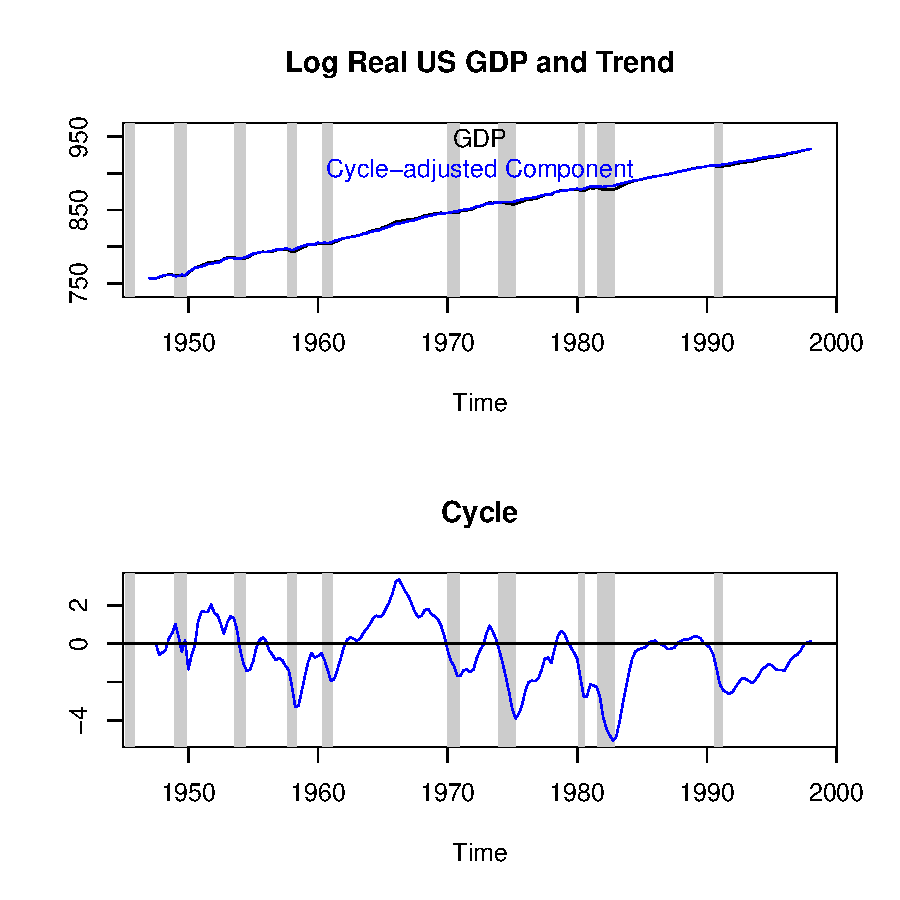
\includegraphics[height=6in, width=6in]{z_us_real_log_gdp_comp}\caption{US Real GDP: Trend (top) and cycle (bottom): data ends in Feb-1998\label{z_us_real_log_gdp_comp}}\end{center}\end{figure}The cycle is similar, but not identical, to the estimate in \href{https://www.dropbox.com/s/1qn5h7s02c86j8i/mnz03.pdf?dl=0}{MNZ (2003)}, fig.1. 
\end{enumerate}


\textbf{Remark}\\
Typically, in applications, the mean duration of the cycle is identified with the argument of the roots of the AR(2)-polynomial: this way we inferred a duration of 12.85 years and, similarly, \href{https://www.dropbox.com/s/1qn5h7s02c86j8i/mnz03.pdf?dl=0}{MNZ (2003)} inferred an `implied period' of 7.82 years, see their table 1. However, as we shall see in section \ref{cf_cr_a_e_cl}, this alleged link between the AR-roots and the effective cycle-length does not apply, in general, because of interference phenomena: the combined effect of both (complex conjugate) roots of the AR-polynomial precludes such an interpretation. Let us foreclose that the spectral densities of \emph{both} AR(2)-cycles (ours and \href{https://www.dropbox.com/s/1qn5h7s02c86j8i/mnz03.pdf?dl=0}{MNZ (2003)}) peak in frequency zero, see fig.\ref{z_effective_length} which suggests a periodicity of infinite length: neither 12.85 nor 7.82 are therefore pertinent cycle-periodicities. In the following we distinguish `implied' and `effective' cycle lengths: the former is the argument of the root of the AR(2)-polynomial and the latter is the peak-frequency of the resulting spectral density. 





\subsection{Adding Recent Data: Validation, Great Recession}

We try to validate the former model by including data up to the onset of the great recession, Dec-2007. Then we assess the impact of the great recession by considering observations up to Nov-2014.

\begin{enumerate}
\item Data:
\begin{Schunk}
\begin{Sinput}
> # Data up to 2008
> end_date<-"2007-12-31"
\end{Sinput}
\end{Schunk}
\begin{Schunk}
\begin{Sinput}
> # Data up to Dec 2014
> end_date<-"2014-11-30"
\end{Sinput}
\end{Schunk}
\item Estimation:
\begin{Schunk}
\begin{Sinput}
> fit2_07 <- dlmMLE(y=lgdp_07,parm=c(1.5303,-.6097,sqrt(.6199),
+                             sqrt(.6893)),build=ssm2,hessian=T)
\end{Sinput}
\end{Schunk}
\begin{Schunk}
\begin{Sinput}
> fit2_14 <- dlmMLE(y=lgdp_14,parm=c(1.5303,-.6097,sqrt(.6199),
+                             sqrt(.6893)),build=ssm2,hessian=T)
\end{Sinput}
\end{Schunk}

Estimates are reported in table \ref{z_ss_uc0_t_gr}. 
% latex table generated in R 3.3.2 by xtable 1.8-2 package
% Fri Dec 16 15:26:07 2016
\begin{table}[ht]
\centering
\begin{tabular}{rrrrrrr}
  \hline
 & Criterion Value & AR(1) & AR(2) & Sigma\_w1 & Sigma\_w2 & `Implied' length (years) \\ 
  \hline
1947-1998 & 109.69 & 1.51 & -0.58 & 0.66 & 0.62 & 12.85 \\ 
  1947-2007 & 112.68 & 1.52 & -0.59 & 0.61 & 0.59 & 13.71 \\ 
  1947-2014 & 121.12 & 1.54 & -0.54 & 0.64 & 0.56 & Inf \\ 
   \hline
\end{tabular}
\caption{Estimates for three different time spans: 1947-1998, 1947-2007, 1947-2014} 
\label{z_ss_uc0_t_gr}
\end{table}We infer that the model is remarkably stable up to the onset of the great recession. Afterwards, the AR(2)-cycle becomes non-stationary (the roots of the AR(2)-polynomial lie on both sides of the unit-circle); accordingly, the `implied' cycle-length is infinite.
\item cycle estimates are plotted in fig.\ref{z_us_real_log_gdp_comp_wgr}.
\begin{figure}[H]\begin{center}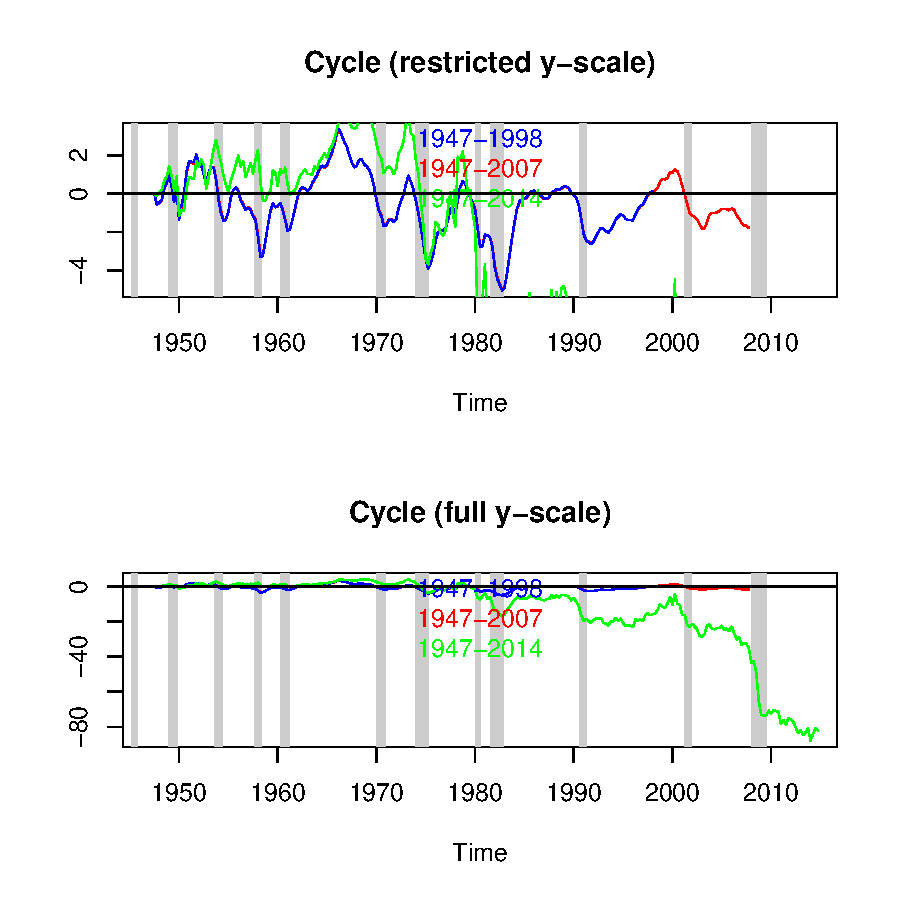
\includegraphics[height=6in, width=6in]{z_us_real_log_gdp_comp_wgr}\caption{Cycles: data up to Feb-1998 (blue), Dec-2007 (red), Dec-2014 (green): restricted scale (top) vs. full scale (bottom)\label{z_us_real_log_gdp_comp_wgr}}\end{center}\end{figure}The `explosive' dynamics of the non-stationary cycle are eminently visible in the bottom panel.
\end{enumerate}
\textbf{Findings}
\begin{itemize}
\item Our two estimates of the AR(2)-cycle, calibrated prior to the great recession, have similar `implied' lengths (roughly 13 years) and the extracted cycle-components are almost indistinguishable, by eye (top panel). 
\item By including the great recession in the estimation span, the cycle-component becomes non-stationary. 
\end{itemize}

\subsubsection{Summary}
\begin{itemize}
\item Numerical optimization of UC- (state space) models is tedious.
\item Short-term forecast performances (maximum likelihood principle) are not well-suited for resolving and discriminating mid-term (cycle) from long-term (trend) dynamics.
\item We were unable to replicate -- exactly -- the results in \href{https://www.dropbox.com/s/1qn5h7s02c86j8i/mnz03.pdf?dl=0}{MNZ (2003)} by the $dlm-$package. In particular the `implied' cycle-lengths, as specified by the roots of the AR(2)-polynomial, differ noticeably. However, both AR(2)-models are essentially similar in the sense that coefficients are not statistically different; moreover, both spectral densities peak in frequency zero, see fig.\ref{z_effective_length}.   
\item Model estimates are fairly stable for data prior to the great recession. 
\item The great recession jumbles components and the cycle becomes non-stationary.
\end{itemize}



\subsection{Implied vs. Effective Cycle-Lengths}\label{cf_cr_a_e_cl}

In the case of \href{https://www.dropbox.com/s/1qn5h7s02c86j8i/mnz03.pdf?dl=0}{MNZ (2003)}, the cycle-component is
\[c_t=1.5303c_{t-1}-0.6097c_{t-2}+\epsilon_t\]
with complex conjugate roots 0.765-0.156i, 0.765+0.156i. The common (absolute) argument of the roots is 0.201 and the duration of a cycle corresponding to this frequency is $\frac{2\pi}{4\cdot0.201}=7.82$ (years). We argue that this number, the `implied' cycle-length as derived from the above calculus, is not a pertinent descriptive statistic of $c_t$, in general. For that purpose we compute the amplitude functions of the two AR(2)-filters specified in table \ref{z_ss_uc0_t}, see fig.\ref{z_effective_length}.
\begin{Schunk}
\begin{Sinput}
> K<-1000
> omega_k<-pi*(0:K)/K
> trffkt_ar2_MNZ<-1/abs(1-1.5303*exp(1.i*omega_k)+0.6097*exp(1.i*2*omega_k))^2
> trffkt_ar2_98<-1/abs(1-fit2_98$par[1]*exp(1.i*omega_k)-fit2_98$par[2]*
+                        exp(1.i*2*omega_k))^2
\end{Sinput}
\end{Schunk}
\begin{figure}[H]\begin{center}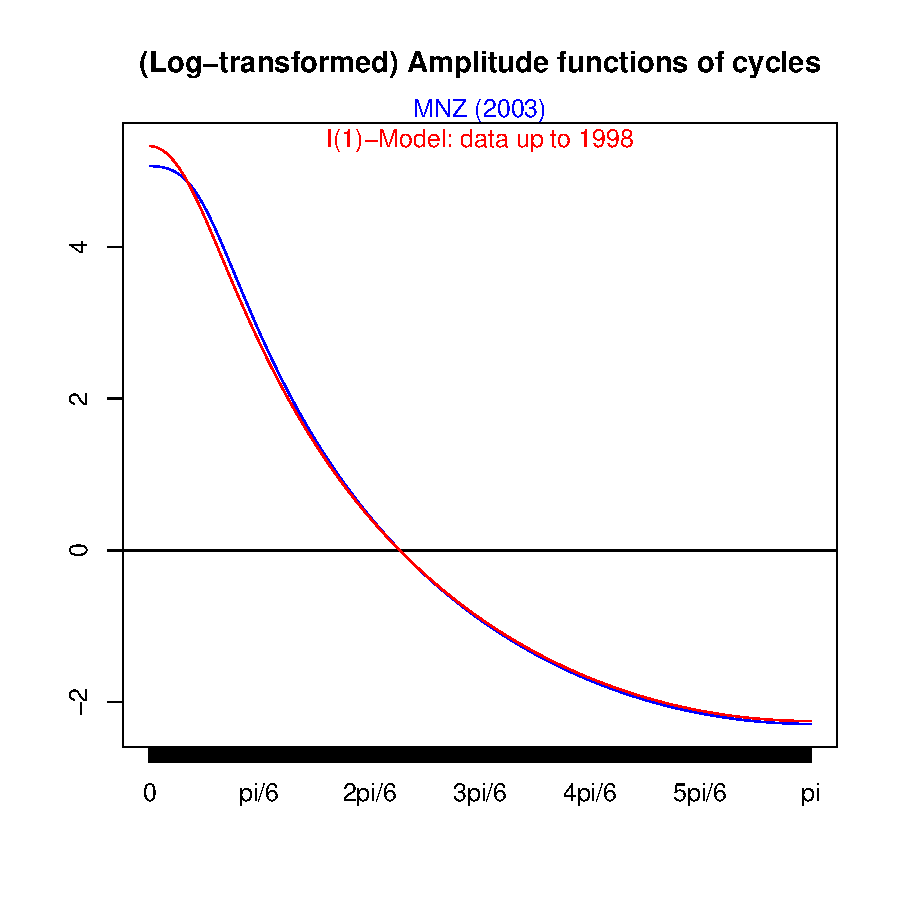
\includegraphics[height=4in, width=6in]{z_effective_length}\caption{(Log-transformed) Amplitude functions of AR(2)-cycles with `implied' cycle-lengths of 8 (blue) and 13  (red) years\label{z_effective_length}}\end{center}\end{figure}Both amplitude functions peak in frequency zero\footnote{The two complex conjugate roots interfer.}: there are no peaks at the alleged `cycle-frequencies' of 8 and 13 years. Accordingly, neither AR(2)-filter or AR(2)-model generates `cycles'. 




\subsection{I(2)-Models: Unconstrained vs. Constrained Cycle-Frequency}

We extend the previous results by fitting model \ref{ss_mod_gen_i2} to the data. Since unconstrained optimization of the likelihood for the general model is an even more challenging task, we here propose four alternative designs:
\begin{enumerate}
\item An unconstrained design: `implied' cycle-length and innovation variances are determined freely.
\item The same model but we impose an `implied'  cycle-length in accordance with the mean duration of business-cycles which is 5.58 years (from 1947 to 2014). To make things simple we impose an implied length of 6 years (24 quarters). 
\item Impose a vanishing level-innovation $\sigma_{w,11}^2=0$.
\item Impose both constraints: `implied' cycle-length of 6 years and  $\sigma_{w,11}^2=0$.
\end{enumerate}
We consider data up to the onset of the great recession only (because the model is not robust).


\subsubsection{Generate Empirical Results}


\begin{enumerate}
\item Read the data:
\begin{Schunk}
\begin{Sinput}
> # Data up to great recession
> end_date<-"2007-12-31"
\end{Sinput}
\end{Schunk}
\item Estimate constrained and unconstrained I(2)-models.  
\begin{Schunk}
\begin{Sinput}
> source(file=paste(path.pgm,"state_space_trend_cycle_gdp.r",sep=""))
\end{Sinput}
\end{Schunk}

\item Estimates and criterion values are to be found in table \ref{z_ss_uc0_t_gr_i2}.
% latex table generated in R 3.3.2 by xtable 1.8-2 package
% Fri Dec 16 15:26:38 2016
\begin{table}[ht]
\centering
\begin{tabular}{rrrrrrr}
  \hline
 & Neg.log-lik & AIC & Duration & s\_33 & s\_11 & s\_22 \\ 
  \hline
Unconstrained & 112.15 & 122.15 & 13.78 & 0.63 & 0.57 & 0.01 \\ 
  Length=6 & 112.61 & 120.61 & 6.00 & 0.57 & 0.61 & 0.01 \\ 
  s\_11=0 & 115.09 & 123.09 & Inf & 0.91 & 0.00 & 0.00 \\ 
  s\_11=0, length=6 & 119.22 & 125.22 & 6.00 & 0.88 & 0.00 & 0.02 \\ 
   \hline
\end{tabular}
\caption{Estimates of I(2)-models: data from 1947 to the onset of the great recession (Dec-2007)} 
\label{z_ss_uc0_t_gr_i2}
\end{table}The columns $s \textunderscore 11, s \textunderscore 22, s \textunderscore 33$ refer to the unknown innovation variances. The AIC-column is obtained by adding twice the number of estimated parameters to the first column (negative log-likelihood): as an example we estimate five parameters in the unconstrained model (first row) which leads to an AIC of $112.146+2*5=122.146$. The resulting information criterion is `informative' about the added-value (pertinence) of freely-determined parameters or of imposed constraints (it is not a formal statistical test, though).
\item Extracted cycle- and drift-components are plotted in fig.\ref{z_us_real_log_gdp_comp_i2}

\begin{figure}[H]\begin{center}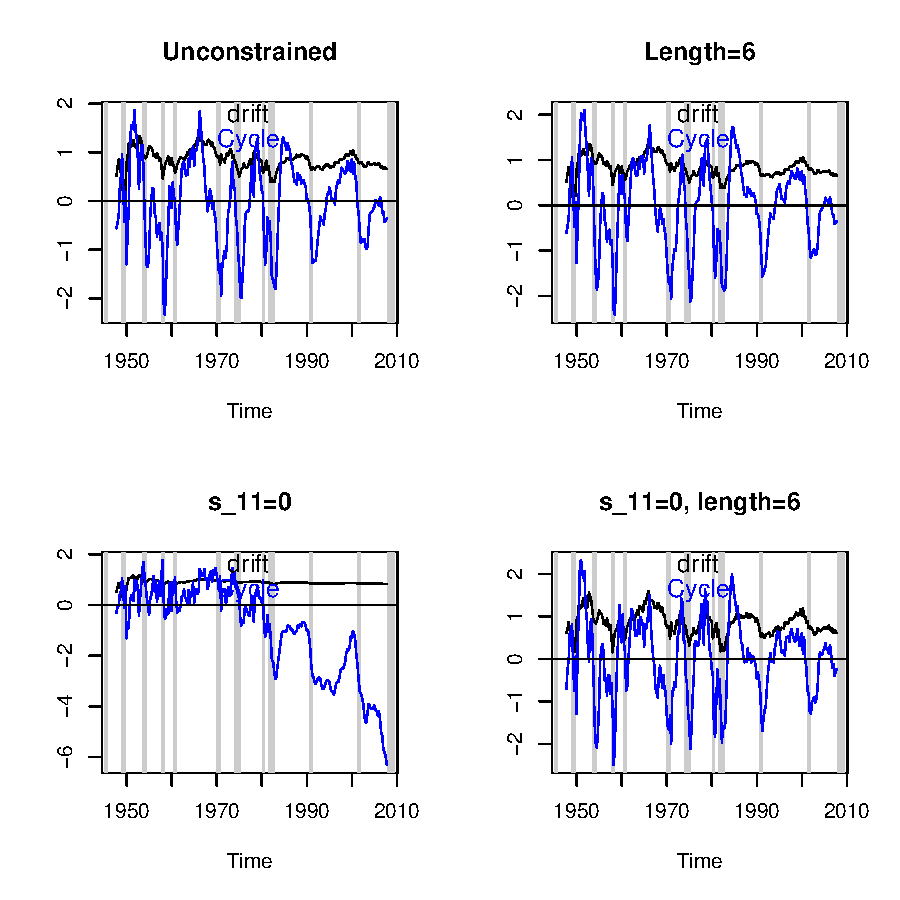
\includegraphics[height=6in, width=6in]{z_us_real_log_gdp_comp_i2}\caption{Cycles and drifts of I(2)-models\label{z_us_real_log_gdp_comp_i2}}\end{center}\end{figure}\end{enumerate}  

\subsubsection{Analysis}
\begin{itemize}
\item Optimization is tedious!
\item Imposing both constraints -- mean cycle-length and $\sigma_{w,11}^2=0$ -- affects the negative log-likelihood (the criterion value) noticeably: the resulting model would be rejected on ground of classical information criteria.
\item The second model, with freely determined innovation variances and imposed cycle-length, fares best according to information criteria. It also (slightly) outperforms the previous I(1)-model, see table \ref{z_ss_uc0_t_gr}. Finally,  the spectral density of the associated cycle does not peak in zero, see section \ref{rep_i2_bp}.
\item The stationary cycles in fig.\ref{z_us_real_log_gdp_comp_i2} (top and bottom-right panels) look similar. Counting-in the I(1)-model in the previous section, this observation may lead one to conclude that neither the integration-order nor the `implied' cycle-length are clearly identified by the data. To some extent, the final decision rests up to the analyst's preference(s). 
\item Fig.\ref{z_us_real_log_gdp_comp_i2} suggests that drift (black line) and cycle (blue line) correlate, against the fact that the model assumes orthogonality of components.  
\end{itemize}
We now return to the main topic and propose to replicate the estimated Trend-Cycle models by DFA. 



\subsection{Replicating the I(1)-Model by DFA}\label{rep_cy_mba_dfa}


We  rely on the I(1)-model estimated in section \ref{mnz_m-gr}, as based on data up to Dec-2007: $\boldsymbol{\theta}=($1.52,-0.585,0.606,0.594). 



\subsubsection{Detrend the Data}

Since the model assumes a constant trend with slope $\mu=$0.85 we first detrend the data, see fig.\ref{z_us_real_log_gdp_detrended}.
\begin{Schunk}
\begin{Sinput}
> drift<-mod2f_07$m[nrow(mod2f_07$m),2]
> trend<-ts(drift*(1:length(lgdp_07)),start=start_year,frequency=4)
> detrended<-lgdp_07-trend
> detrended<-detrended-mean(detrended)
\end{Sinput}
\end{Schunk}
\begin{figure}[H]\begin{center}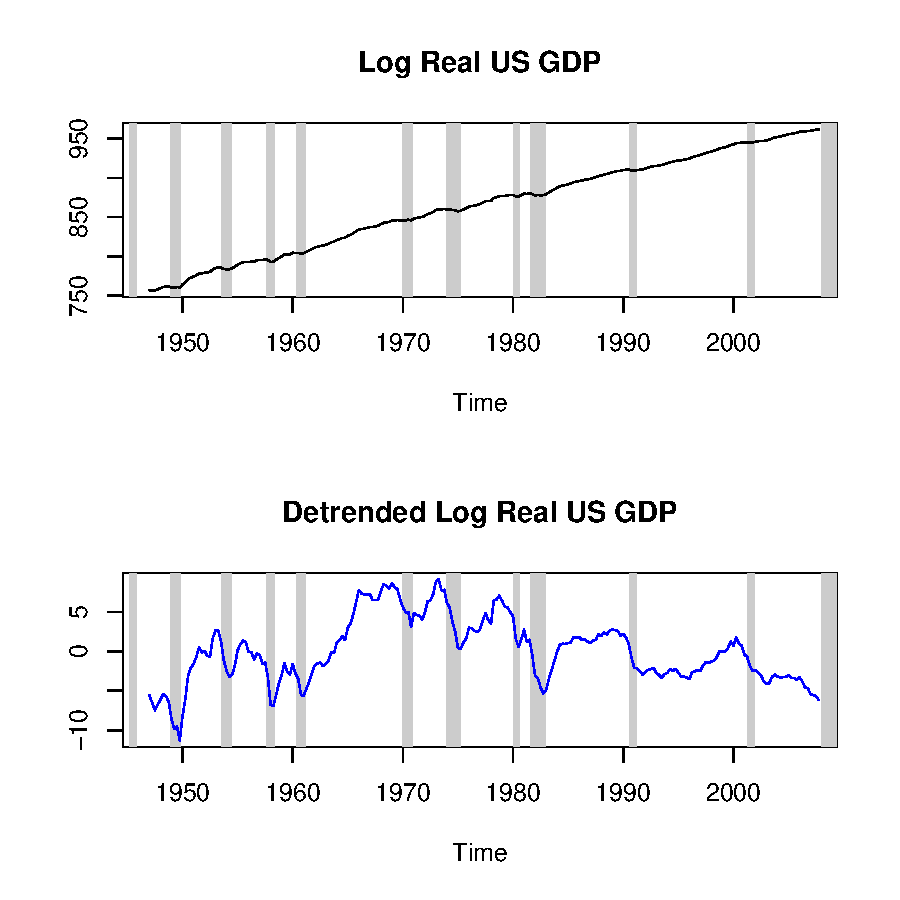
\includegraphics[height=6in, width=6in]{z_us_real_log_gdp_detrended}\caption{GDP (top) and trend-adjusted GDP (bottom)\label{z_us_real_log_gdp_detrended}}\end{center}\end{figure}Centering the detrended series about zero, as we did in the bottom panel, is facultative and does not affect results. 







\subsubsection{DGP and Replication}



The DGP of the detrended series in fig.\ref{z_us_real_log_gdp_detrended} is (assumed to be) the sum of a random-walk (without drift) and of a stationary stochastic cycle. Since the latter two components are independent, by assumption, the (pseudo-) spectral density of the DGP is obtained by summing-up both components
\begin{eqnarray*}
h_{cycle}(\omega)&=&\frac{\sigma_{w,22}^2}{|1-a_1\exp(i\omega)-a_2\exp(i2\omega)|^2}\\
h_{trend}(\omega)&=&\frac{\sigma_{w,11}^2}{|1-\exp(i\omega)|^2}\\
h_{Detrended~GDP}(\omega)&=&h_{cycle}(\omega)+h_{trend}(\omega)
\end{eqnarray*}
Specifically
\[h_{Detrended~GDP}(\omega):=\frac{0.37}{|1-\exp(-i\omega)|^2}+\frac{0.35}{|1-1.52\exp(-i\omega)+0.59\exp(-i2\omega)|^2}\]
see fig.\ref{z_us_real_log_gdp_detrended_spect} (the singularity in frequency zero has been skipped).
\begin{figure}[H]\begin{center}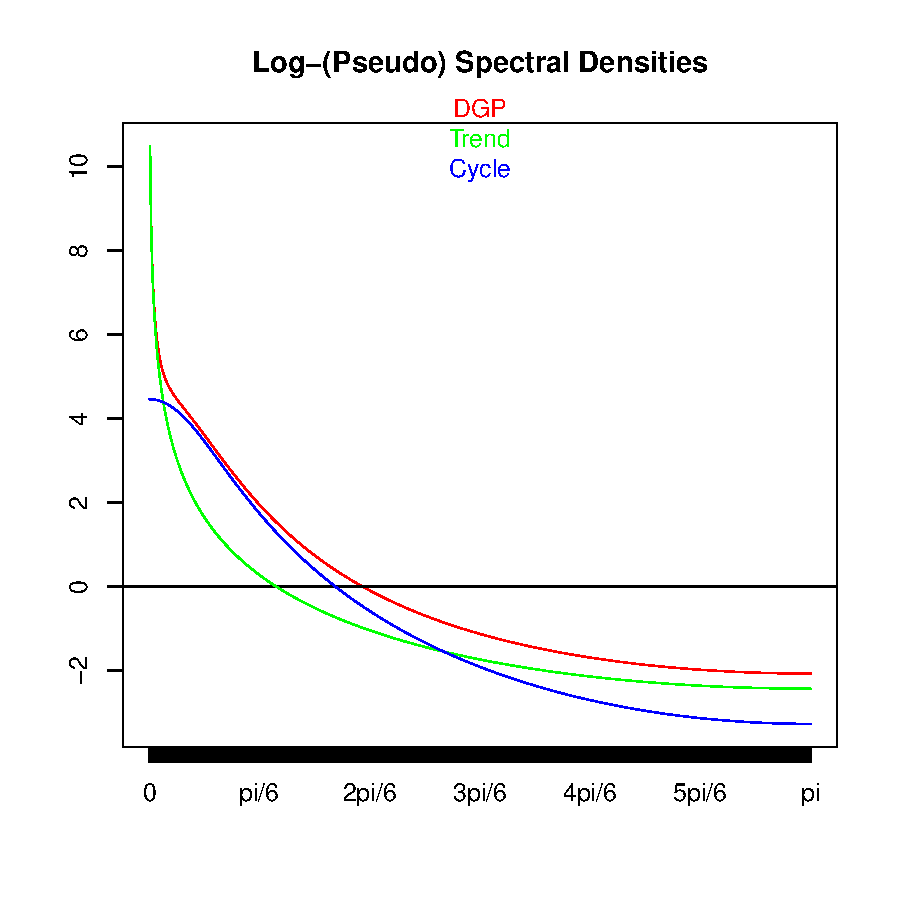
\includegraphics[height=4in, width=4in]{z_us_real_log_gdp_detrended_spect}\caption{Log (pseudo) spectral densities of DGP (red), trend (green) and cycle (blue) \label{z_us_real_log_gdp_detrended_spect}}\end{center}\end{figure}The pseudo-spectral density of the DGP (red line) can be plugged into \ref{dfa_ms} but the unit-root requires a first-order restriction, $i1=T$, recall section \ref{pseudo_dft}\footnote{See chapter \ref{int_sec} for a formal treatment.}. In order to focus on the interesting business-cycle we address a bandpass target.







\subsubsection{Bandpass Target}


Model \ref{ss_mod_gen_i2} and its nested variant \ref{ss_mod_gen_i1} generate model-based (symmetric) target filters. As an alternative, we here rely on a classic `2-10 years' business-cycle design
\begin{eqnarray}\label{ideal_bp_t}
\Gamma(\omega)&=&\left\{\begin{array}{cc}1~&~\frac{\pi}{20}\leq |\omega|\leq \frac{\pi}{4}\\
0~&~\textrm{otherwise}\end{array}\right.
\end{eqnarray}
where the cutoff-frequencies refer to quarters. This way, our research priorities are matched explicitly by the target specification. \\




Next, we compare outputs of the previous I(1)- and I(2)-models with the new (real-time) bandpass design, assuming $L=100$. Since the DGP is assumed to be integrated of order one, we impose a simple level constraint $i1=T$, see section \ref{first_order_cons}. 
\begin{enumerate}
\item Specify the filter design: cutoff, restriction ($i1=T$), MSE-design ($\lambda=\eta=0$).
\begin{Schunk}
\begin{Sinput}
> cutoff_len_upper<-4
> cutoff_len_lower<-20
> cutoff_upper<-pi/cutoff_len_upper
> L<-100
> # Spectrum: MDFA requires DFT i.e. square-root of density 
> # The design is univariate i.e. input and output series are synchronized.
> # Therefore we can rely on absolute values (no phase information 
> #   is required).
> weight_func<-cbind(sqrt(trffkt_GDP),sqrt(trffkt_GDP))
> # Ignore singularity in frequency zero 
> weight_func[1,]<-0
> # Target
> Gamma<-(0:K)<=as.integer(cutoff_upper*K/pi)+1
> Gamma[1:(K/cutoff_len_lower+1)]<-0
> # Restrictions: i1 constraint
> i1<-T
> i2<-F
> weight_constraint<-Gamma[1]
> # MSE-design
> lambda<-eta<-0
\end{Sinput}
\end{Schunk}
\item Proceed to estimation:
\begin{Schunk}
\begin{Sinput}
> # Estimate MDFA MSE filter coefficients  
> mdfa_obj<-mdfa_analytic(L,lambda,weight_func,Lag,Gamma,eta,cutoff,
+                   i1,i2,weight_constraint,lambda_cross,lambda_decay,
+                   lambda_smooth,lin_eta,shift_constraint,grand_mean,
+                   b0_H0,c_eta,weight_structure,
+                   white_noise,synchronicity,lag_mat,troikaner)
\end{Sinput}
\end{Schunk}
Note that we could replicate this object by the simpler context-specific call
\begin{Schunk}
\begin{Sinput}
> # Estimate MDFA MSE filter coefficients  
> mdfa_obj<-MDFA_mse_constraint(L,weight_func,Lag,Gamma,i1,i2,weight_constraint,
+                               shift_constraint)$mdfa_obj
\end{Sinput}
\end{Schunk}
whereby $MDFA\textunderscore mse\textunderscore constraint$ handles constrained MSE-designs, specifically.

\item Compute amplitude and time-shift functions, see fig.\ref{z_us_real_log_gdp_detrended_amp_shift_bp}: the time-shift is restricted to the passband only.
\begin{figure}[H]\begin{center}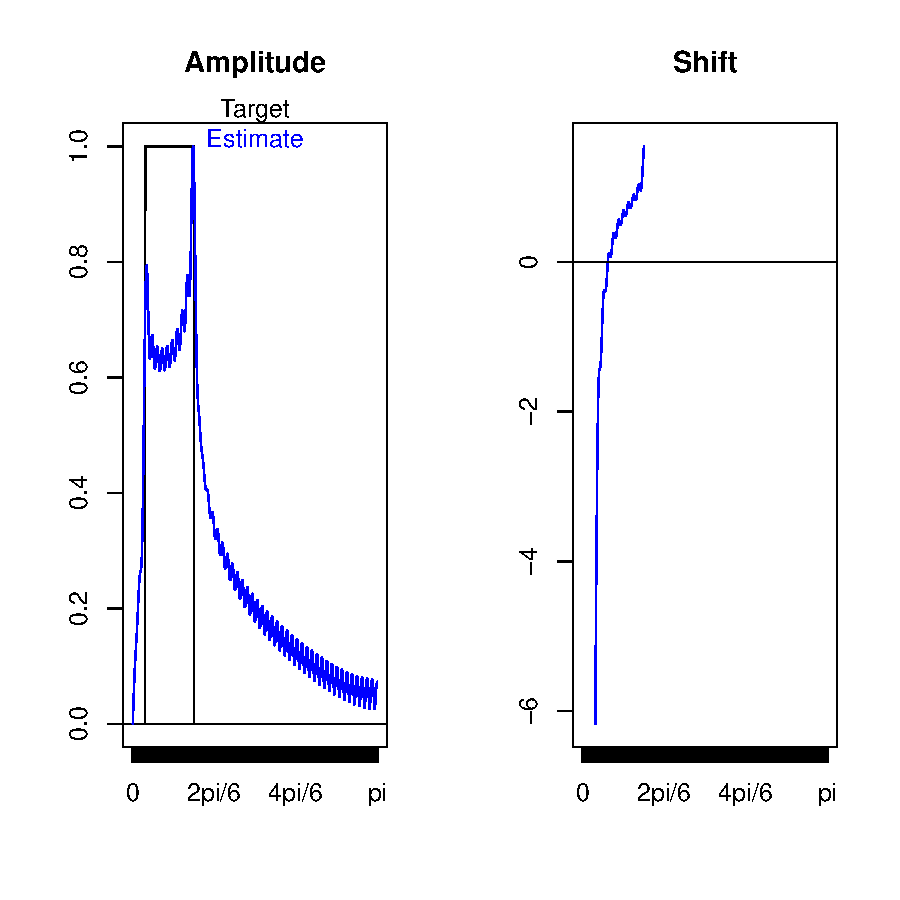
\includegraphics[height=4in, width=6in]{z_us_real_log_gdp_detrended_amp_shift_bp}\caption{Amplitude (left) and time-shift functions of real-time bandpass MSE-design, i1=T\label{z_us_real_log_gdp_detrended_amp_shift_bp}}\end{center}\end{figure}The observed ripples are innocuous: they are due to the discontinuity of the ideal bandpass which cannot be fitted perfectly by a finite-length filter ($L=100$).  
\item Compute the bandpass-MSE filter-output; compare cycles of I(1)-model (fig.\ref{z_us_real_log_gdp_comp_wgr}), best I(2)-model (fig.\ref{z_us_real_log_gdp_comp_i2}, top-right panel) and bandpass-MSE, see fig.\ref{z_us_real_log_gdp_detrended_filt_bp}.

\begin{Schunk}
\begin{Sinput}
> xf_i1<-rep(NA,length(detrended))
> for (i in L:length(detrended))  
+   xf_i1[i]<-t(mdfa_obj$b)%*%(detrended[i:(i-L+1)]-mean(detrended))  
\end{Sinput}
\end{Schunk}


\begin{figure}[H]\begin{center}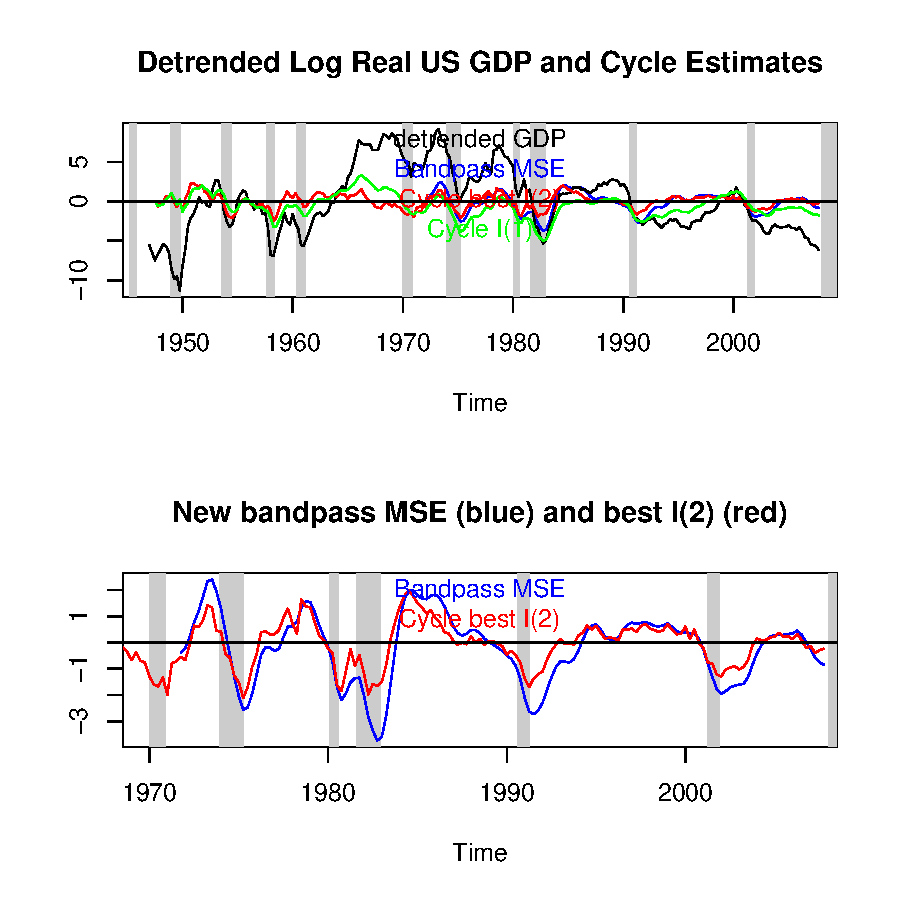
\includegraphics[height=6in, width=6in]{z_us_real_log_gdp_detrended_filt_bp}\caption{Detrended (log-real) US-GDP (black), new bandpass MSE (blue), best I(2)-model (red) and I(1)-model (green)   \label{z_us_real_log_gdp_detrended_filt_bp}}\end{center}\end{figure}\end{enumerate}
The new MSE-bandpass (blue line) fares well: it tracks expansions and recessions similarly to the best I(2)-model (red line). The former is a bit smoother and slightly delayed when compared to the latter: further customization could address both issues, at once.




\subsection{Replicating the General I(2)-Model by DFA}\label{rep_cy_mba_dfa_i2}


\subsubsection{DGP and Pseudo-Spectrum}\label{rep_i2_bp}

If $\sigma_{w,22}^2>0$ in the general model \ref{ss_mod_gen_i2}, then the DGP has a double unit-root in frequency zero. Its pseudo-spectrum is obtained by summing-up the spectra corresponding to the three orthogonal innovation processes
\begin{eqnarray*}
h_{cycle}(\omega)&=&\frac{\sigma_{w,33}^2}{|1-a_1\exp(i\omega)-a_2\exp(i2\omega)|^2}\\
h_{level}(\omega)&=&\frac{\sigma_{w,11}^2}{|1-\exp(i\omega)|^2}\\
h_{drift}(\omega)&=&\frac{\sigma_{w,22}^2}{|1-\exp(i\omega)|^4}\\
h_{DGP}(\omega)&=&h_{cycle}(\omega)+h_{level}(\omega)+h_{drift}(\omega)
\end{eqnarray*}
For the best I(2)-model (top right panel in fig.\ref{z_us_real_log_gdp_comp_i2}) we obtain
\[
h_{DGP}(\omega)=\frac{0.33}{|1-1.53\exp(i\omega)+0.63\exp(i2\omega)|^2}+
\frac{0.37}{|1-\exp(i\omega)|^2}+\frac{0.000125}{|1-\exp(i\omega)|^4}
\]
see fig.\ref{z_us_real_log_gdp_detrended_spect_i2}.
\begin{figure}[H]\begin{center}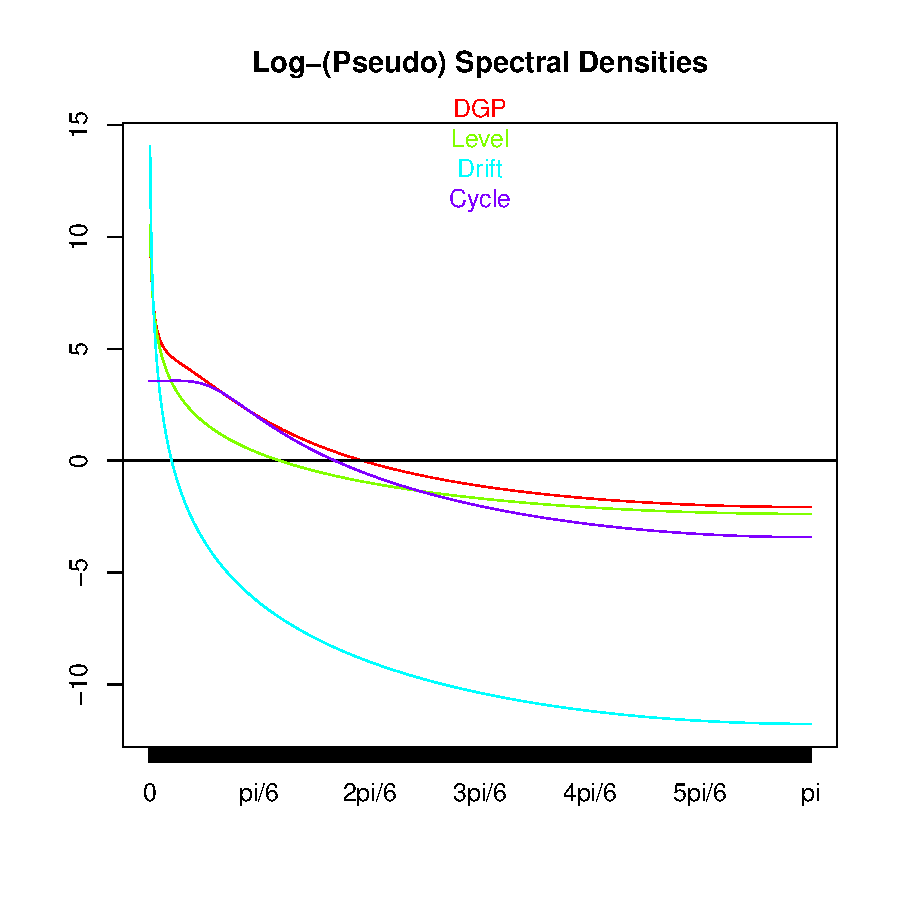
\includegraphics[height=4in, width=6in]{z_us_real_log_gdp_detrended_spect_i2}\caption{Log (pseudo) spectral densities of DGP (red), level (green), drift (cyan) and cycle (violet) \label{z_us_real_log_gdp_detrended_spect_i2}}\end{center}\end{figure}Note that the cycle-spectrum (violet) peaks in $\displaystyle{\frac{\pi}{24.39}}$ which corresponds to an effective (mean) cycle-length of 12.2 years (we imposed an `implied' length of 6 years); the peak is very flat, though. The drift (cyan) is dominated by the sum of the cycle (violet) and of the level (green) on most of the frequency-band, except in a very narrow band centered about zero (the drift is slowly changing i.e. $\sigma_{w,22}$ is very small). As a result, the pseudo-spectral density of the I(1)-model in the previous section (fig.\ref{z_us_real_log_gdp_detrended_spect}) and of the current I(2)-model look similar. Therefore, we expect that the resulting cycle-estimates should be similar, too. \\
The MBA can be replicated by the DFA by plugging $h_{DGP}(\omega)$ into \ref{dfa_ms}. Since the process is integrated of order two, we have to impose first \emph{and} second-order filter constraints, see section \ref{pseudo_dft}.  





\subsubsection{Ideal Bandpass}

As in the previous section \ref{rep_cy_mba_dfa} we here target an ideal 2-10 years bandpass. In contrast to the previous section, however, the data does not need to be detrended: the drift is stochastic and the DGP is an I(2) process. Another distinguishing feature is that we propose an unconstrained design based on the following MSE-criterion
\begin{eqnarray*}
\frac{2\pi}{T}\sum_{k=-M}^{M}\left|\Gamma(\omega_k)-\hat{\Gamma}(\omega_k) (1-\exp(-i\omega_k))^2\right|^2 h_{GDP}(\omega_k)\to\min_{\mathbf{b}} 
\end{eqnarray*}
The composite filter $\hat{\Gamma}(\omega_k) (1-\exp(-i\omega_k))^2$ consists of a double difference filter, which transforms an I(2)-process into a stationary time series, and an unconstrained $\hat{\Gamma}(\omega_k)$ which `undistords' the double difference such that the composite design matches the bandpass target $\Gamma(\cdot)$ for $\omega_k>0$. The composite filter satisfies the required I(2)-constraint, by construction, and irrespective of the finite MA-filter $\hat{\Gamma}(\cdot)$, and therefore the above criterion is well defined (the singularity in frequency zero is cancelled\footnote{Note that the ideal bandpass target $\Gamma(\omega_k)$ has a zero of infinite order in frequency zero.}). For convenience we rewrite the criterion as follows 
\begin{eqnarray*}
\frac{2\pi}{T}\sum_{k=-M}^{M}\left|\Gamma(\omega_k)\sqrt{h_{GDP}(\omega_k)}-\hat{\Gamma}(\omega_k)\bigg[\sqrt{h_{GDP}(\omega_k)} (1-\exp(-i\omega_k))^2\bigg]\right|^2 \to\min_{\mathbf{b}} 
\end{eqnarray*}
The target variable relies on original data in levels; but the explanatory variable relies on second-order differences, as emphasized by the bracketed (square-root) spectral density\footnote{Note that $\sqrt{h_{GDP}(\omega_k)} (1-\exp(-i\omega_k))^2$ is complex-valued: the second-order differences affect the phase relative to the target.}.
\begin{enumerate}
\item Specify the filter design and feed the (pseudo-) spectral density to MDFA.
\begin{Schunk}
\begin{Sinput}
> cutoff_len_upper<-4
> cutoff_len_lower<-20
> cutoff_upper<-pi/cutoff_len_upper
> L<-100
> # Spectrum: the second-order difference filter is applied to the 
> # explanatory variable (second column) 
> #   Important: the relative phase information between target (data in level)
> #   and explanatory variable (differenced data) is required.
> #   Therefore one must supply the transferfunction (not the amplitude) 
> #   of the differenced filter!
> weight_func<-cbind(sqrt(trffkt_i2_GDP),sqrt(trffkt_i2_GDP)*(1-exp(1.i*omega_k))^2)
> # Ignore singularity in frequency zero
> weight_func[1,]<-0
> # Target
> Gamma<-(0:K)<=as.integer(cutoff_upper*K/pi)+1
> Gamma[1:(K/cutoff_len_lower+1)]<-0
> # Unconstrained design: the zero of order 2 is already obtained
> #   by the double difference filter
> i1<-F
> i2<-F
> # MSE-design
> lambda<-eta<-0
\end{Sinput}
\end{Schunk}
\item estimation:
\begin{Schunk}
\begin{Sinput}
> # Estimate MDFA MSE filter coefficients  
> mdfa_obj<-mdfa_analytic(L,lambda,weight_func,Lag,Gamma,
+               eta,cutoff,i1,i2,weight_constraint,lambda_cross,
+               lambda_decay,lambda_smooth,lin_eta,shift_constraint,
+               grand_mean,b0_H0,c_eta,
+               weight_structure,white_noise,synchronicity,lag_mat,troikaner)
\end{Sinput}
\end{Schunk}
Note that this object could be replicated by the simpler context-specific call
\begin{Schunk}
\begin{Sinput}
> mdfa_obj<-MDFA_mse(L,weight_func,Lag,Gamma)$mdfa_obj
\end{Sinput}
\end{Schunk}
where $MDFA\textunderscore mse$ can handle the simplest (unconstrained) MSE case.
\item Compute amplitude and time-shift functions of the \emph{composite} filter, see fig.\ref{z_us_real_log_gdp_detrended_amp_shift_bp_i2}: the time-shift is restricted to the passband only.
\begin{figure}[H]\begin{center}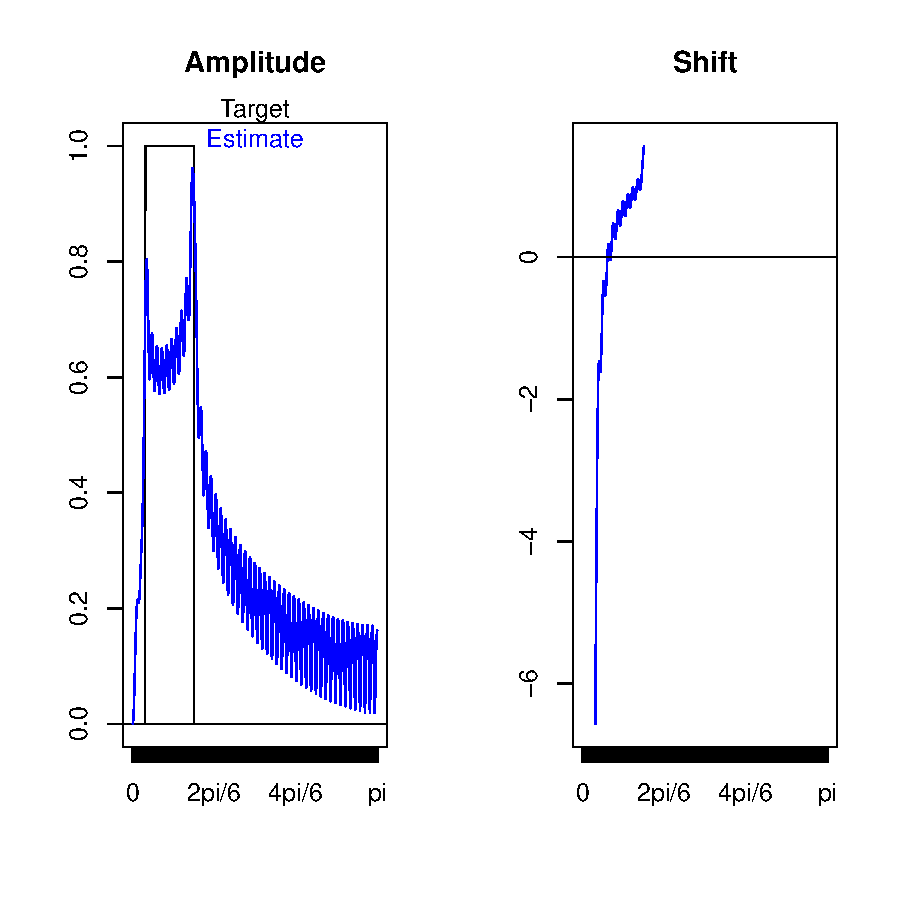
\includegraphics[height=4in, width=6in]{z_us_real_log_gdp_detrended_amp_shift_bp_i2}\caption{Amplitude (left) and time-shift functions (right) of real-time composite unconstrained bandpass MSE-design\label{z_us_real_log_gdp_detrended_amp_shift_bp_i2}}\end{center}\end{figure}As in the previous section, the observed ripples are innocuous (approximation of ideal bandpass target by finite-length filter). 
\item Compute the output of the \emph{composite} bandpass-MSE filter. Compare cycles of I(1)-model (fig.\ref{z_us_real_log_gdp_comp_wgr}), best I(2)-model (fig.\ref{z_us_real_log_gdp_comp_i2}, top-right panel), and composite bandpass, see fig.\ref{z_us_real_log_gdp_detrended_filt_bp_i2}.

\begin{Schunk}
\begin{Sinput}
> xf_i2<-rep(NA,length(detrended))
> # Apply second-order differences to the data
> diff2_lgdp_07<-c(0,0,diff(lgdp_07,diff=2))
> for (i in L:length(detrended))  
+   xf_i2[i]<-t(mdfa_obj$b)%*%diff2_lgdp_07[i:(i-L+1)]  
\end{Sinput}
\end{Schunk}


\begin{figure}[H]\begin{center}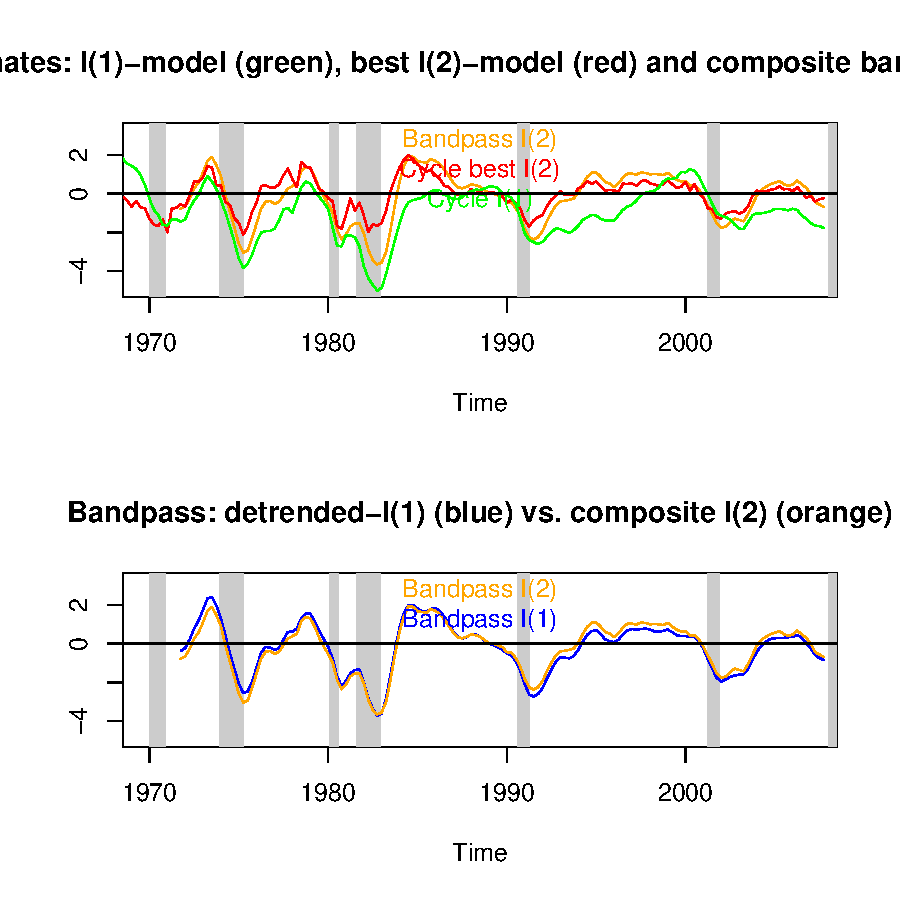
\includegraphics[height=6in, width=6in]{z_us_real_log_gdp_detrended_filt_bp_i2}\caption{Composite bandpass (orange), bandpass I(1) (blue), best I(2)-model (red) and I(1)-model (green)   \label{z_us_real_log_gdp_detrended_filt_bp_i2}}\end{center}\end{figure}\end{enumerate}
\textbf{Analysis}
\begin{itemize}
\item Both bandpass designs as well as the best I(2)-model generate zero-centric cycles which follow the alternating expansion and contraction episodes. 
\item The two bandpass (DFA) MSE-estimates are nearly identical despite different unit-root specifications or data transformation (detrending in the I(1)-case). This is because the pseudo-spectral densities of the DGP behave similarly outside a narrow band centered at the unit root frequency zero, recall section \ref{rep_i2_bp}.
\item The cycle of the best I(2)-model (red) appears to trade smoothness against speed: the series is a bit noisier but turning points  are detected earlier. Both issues could be tackled at once by suitable customization of the replicated MBA.
\end{itemize}





\section{Customization of UC-Models}\label{cust_uc_mod}

Once replicated by the DFA, the above trend-cycle models could be customized. However, since the model specification is sensitive to singular events, in particular to the protracted down-turn during the great recession, we here propose to analyze more robust designs, namely the classic Hodrick-Prescott and Christiano-Fitzgerald filters, which are replicated and customized by MDFA. 






\section{Replication and Customization of the Hodrick-Prescott HP-Filter)}\label{rep_cust_cl_fi_d}

\subsection{Replication}


The HP-filter is widely used in macroeconomics, for trend extraction or for business-cycle analysis. The original optimization principle 
\begin{eqnarray*}
\frac{1}{T} \sum_{t=1}^T (x_t-y_t)^2+\lambda_{HP} \sum_{t=3}^T [(1-B)^2y_t]^2\to \min_{y_t}
\end{eqnarray*}
where $x_t$ is the data, $y_t$ is the HP-trend and $\lambda_{HP}>0$ is a regularization term, was proposed by Whittaker (1923): the parameter $\lambda_{HP}$ balances a trade off between data-fitting (left term) and smoothness (right term), whereby the squared second order differences $[(1-B)^2y_t]^2$ of the trend correspond to the Curvature measure introduced in section \ref{peco_cu} (omitting the normalization in the latter expression). For $\lambda_{HP}=0$ the trend $y_t$ (over)fits the data perfectly and for $\lambda_{HP}=\infty$ the trend is a linear function of time $t$ (the curvature vanishes). For quarterly data, Hodrick and Prescott have proposed to select $\lambda_{HP}=1600$. \\

The solution of the above minimization problem can be interpreted in terms of a formal signal extraction problem, see 
\href{https://www.dropbox.com/s/dwdx0fcys34g9ku/maravall_kaiser.pdf?dl=0}{Maravall and Kaiser (2004)} and 
\href{https://www.dropbox.com/s/s8zb0buqzygefby/mcelroy_hp.pdf?dl=0}{McElroy (2008)}. In this framework the HP-trend $y_t$ is the output of a symmetric filter\footnote{We here assume that $y_t$ is estimated in the middle of a large sample, such that symmetric filters can be applied.}:
\[y_t=\frac{q}{q+(1-B)^2(1-F)^2}x_t\]
where $q=1/\lambda_{HP}$ and where $F=B^{-1}$ is the forward operator. The implicit model underlying the approach assumes that
\begin{eqnarray*}
x_t&=&T_t+\lambda_{HP} I_t\\
(1-B)^2T_t&=&\nu_t
\end{eqnarray*}
where $I_t,\nu_t$ are mutually independent Gaussian white noise sequences with identical variances. In this case, i.e. if the model applies, $y_t$ is an optimal MSE estimate of the unobserved trend $T_t$. Note that $\lambda_{HP}$ can be interpreted as an inverse SNR: for $\lambda_{HP}=0$ the noise vanishes and therefore $x_t=T_t$ or, equivalently, $y_t=x_t$. For $\lambda_{HP}=1600$ the DGP of $x_t$ is found to be 
\begin{eqnarray}\label{implicit_mode_ass}
(1-B)^2x_t=(1-1.7771B+0.7994B^2)\epsilon_t
\end{eqnarray}
where $\epsilon_t$ is Gaussian white noise, see \href{https://www.dropbox.com/s/dwdx0fcys34g9ku/maravall_kaiser.pdf?dl=0}{Maravall and Kaiser (2004)} and \href{https://www.dropbox.com/s/s8zb0buqzygefby/mcelroy_hp.pdf?dl=0}{McElroy (2008)}\footnote{The latter author provides R-code for an exact derivation of the MA-parameters as a function of $\lambda_{HP}$, see section \ref{hp_exe_repli} below.}. The corresponding implicit pseudo-spectral density is
\begin{eqnarray}\label{hp_pseudo_spec}
h(\omega)=\sigma^2\left|\frac{1-1.7771\exp(-i\omega)+0.7994\exp(-i2\omega)}{(1-\exp(-i\omega))^2}\right|^2
\end{eqnarray}
where $\sigma^2$ is the variance of $\epsilon_t$. Note that the filter-coefficients are invariant to the scale of the data  and therefore we may set $\sigma^2=1$, without affecting estimation results. The target, i.e. the symmetric HP-trend filter, could be obtained in R by relying on the so-called mFilter-library 
\begin{Schunk}
\begin{Sinput}
> # Call HP-routines
> library(mFilter)
\end{Sinput}
\end{Schunk}
We conclude that optimality of the HP-trend, in terms of the MSE-metric, is reliant on an implicit model representation of the data. The corresponding DGP is integrated of order two, I(2), and its parameters are uniquely determined by the (inverse) SNR $\lambda_{HP}$.



\subsection{Exercises: Replication}\label{hp_exe_repli}



Since the HP-filter is less affected by the great recession than the previous state space models we do not skip recent data i.e. we consider the whole GDP series. 
\begin{enumerate}
\item Load the full GDP-series, starting in 1960.
\begin{Schunk}
\begin{Sinput}
> # Load full data-set
> start_year<-1960
> end_date<-format(Sys.time(), "%Y-%m-%d")
> end_year<-as.double(substr(end_date,1,4))
> start_date=paste(start_year,"-01-01",sep="")
> # Select data between start_year and end_year
> data_sample<-mydata[paste("/",end_date,sep="")]
> data_sample<-data_sample[paste(start_date,"/",sep="")]
> lgdp <- ts(100*log(data_sample),start=start_year,frequency=4)
> nobs <- length(lgdp)
\end{Sinput}
\end{Schunk}
\item Load the R-function for deriving the MA-coefficients of the implicit time series model of the HP-filter, see \href{https://www.dropbox.com/s/s8zb0buqzygefby/mcelroy_hp.pdf?dl=0}{McElroy (2008)}.
\begin{Schunk}
\begin{Sinput}
> source(file=paste(path.pgm,"hpFilt.r",sep=""))
> head(hpFilt)
\end{Sinput}
\begin{Soutput}
1 function (q, n)                                                  
2 {                                                                
3     absZ <- (sqrt(q) + sqrt(q + 16) + sqrt(2 * q + 2 * sqrt(q) * 
4         sqrt(q + 16)))/4                                         
5     c <- q/(absZ^2)                                              
6     theta <- atan(sqrt(2 * q + 2 * sqrt(q) * sqrt(q + 16))/4)    
\end{Soutput}
\end{Schunk}
The parameters $q$ and $n$ in the head of the function-call correspond to $1/\lambda_{HP}$ and $L$, the filter-length.
\item \label{exe_hpcode_tuck}Verify that the function replicates the implicit model in the case $\lambda_{HP}=1600$. Hint: for the filter length we select the length of the GDP-series.
\begin{Schunk}
\begin{Sinput}
> # Data: US-GDP
> x<-lgdp
> # Series length
> len<-L_hp<-length(x)
> # Select lambda
> lambda_hp<-1600
> q<-1/lambda_hp
> hp_filt_obj<-hpFilt(q,L_hp)
> tail(hpFilt,2)
\end{Sinput}
\begin{Soutput}
21     return(list(filter_coef = filter_coef, ma_model = ma_model))
22 }                                                               
\end{Soutput}
\begin{Sinput}
> hp_filt_obj$ma_model
\end{Sinput}
\begin{Soutput}
[1]  0.0004996524 -1.7770908783  0.7994437833
\end{Soutput}
\begin{Sinput}
> ma_coeff<-hp_filt_obj$ma_model[2:3]
\end{Sinput}
\end{Schunk}
The first model-coefficient is a normalizing constant, which is irrelevant for our application, and the remaining two parameters correspond to the MA(2)-part of the model. The function computes filter coefficients and implicit model-parameters for any $q=1/\lambda_{HP}$. 
\item Set $\lambda_{HP}=1600$ (quarterly data) and apply the filter, as implemented 
in the $mFilter$ package, see fig.\ref{z_HP_us_real_log_gdp}.
\begin{Schunk}
\begin{Sinput}
> # Resolution of frequency-grid: 2-times the sample length
> #   Selecting a higher resolution would tighten the approximation of HP by DFA
> K<-2*len
> # proceed to filtering
> x_hp <- hpfilter(x,type="lambda", freq=lambda_hp)
> # Extract the coefficients of the symmetric trend:
> #   hpfilter generates coefficients of the HP-gap (see below):
> #   we here transform back to trend filter
> parm<-diag(rep(1,len))-x_hp$fmatrix
> file = paste("z_HP_us_real_log_gdp.pdf", sep = "")
> pdf(file = paste(path.out,file,sep=""), paper = "special", width = 6, 
+     height = 6)
> # Plots: filter coefficients and series
> par(mfrow=c(2,1))
> title_more<-NA
> mplot<-cbind(parm[,len/2],parm[,1])
> plot_title<-"HP lambda=1600: symmetric (red) and real-time (blue)"
> axis_d<-1:len-1
> insamp<-1.e+99
> colo<-c("red","blue")
> mplot_func(mplot,axis_d,plot_title,title_more,insamp,colo)
> mplot<-cbind(rep(NA,len),rep(NA,len),rep(NA,len),x,x_hp$trend)
> plot_title<-"Log US-GDP (blue) vs HP-Trend (red)"
> plot(mplot[,4],col="blue",xlab="",ylab="",main=plot_title)
> nberShade()
> lines(mplot[,5],col="red")
> invisible(dev.off())
\end{Sinput}
\end{Schunk}
\begin{figure}[H]\begin{center}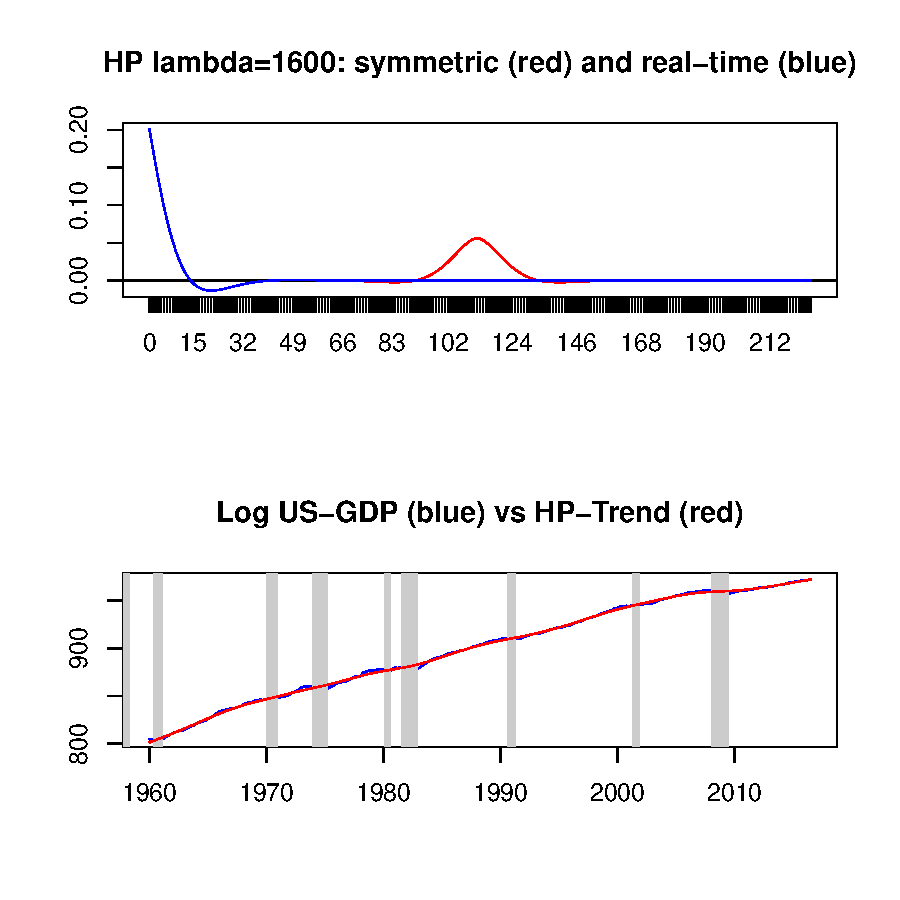
\includegraphics[height=6in, width=6in]{z_HP_us_real_log_gdp}\caption{Filter coefficients of HP-trend, lambda=1600: symmetric (red) and real-time (blue) filters (top-graph). Original and filtered log US-GDP (bottom figure) \label{z_HP_us_real_log_gdp}}\end{center}\end{figure}\item Compute the target signal, corresponding to the symmetric HP-filter, and the pseudo-spectral density \ref{hp_pseudo_spec}, see fig.\ref{z_HP_filt_trffkt}.
\begin{Schunk}
\begin{Sinput}
> # Compute pseudo-spectral density underlying Wiener-Kolmogorov derivation of HP 
> #   (see McElroy (2008) or Maravall-Kaiser p.179)
> # For lambda=1600 the MA coefficients are -1.77709 and 0.79944
> # Note that MDFA is fed with the square-root of the spectrum
> #   (this would correspond to the absolute value of the DFT)
> weight_func_h<-abs((1+ma_coeff[1]*exp(-1.i*(0:(K))*pi/(K))+
+                       ma_coeff[2]*exp(-1.i*2*(0:(K))*pi/(K)))/
+                       (1-exp(-1.i*(0:(K))*pi/(K)))^2)
> # Specify (square-root) spectra of target (first column) 
> #   and of explanatory variable (second column): target and 
> #   explanatory are the same here (univariate filter)
> weight_func<-cbind(weight_func_h,weight_func_h)
> # Compute target Gamma: HP-trend symmetric filter, see McElroy (2008)
> Gamma<-0:(K)
> for (k in 0:(K))
+ {
+   omegak<-k*pi/(K)
+   Gamma[k+1]<-(1/lambda_hp)/(1/lambda_hp+abs(1-exp(1.i*omegak))^4)
+ }
> file = paste("z_HP_filt_trffkt.pdf", sep = "")
> pdf(file = paste(path.out,file,sep=""), paper = "special", width = 6, 
+     height = 6)
> par(mfrow=c(2,1))
> colo<-c("blue","red")
> insamp<-1.e+99
> mplot<-as.matrix(Gamma)
> plot_title<-"Target Gamma, lambda=1600"
> freq_axe<-rep(NA,K+1)
> freq_axe[1]<-0
> freq_axe[1+(1:6)*K/6]<-c(paste(c("",2:5),"pi/6",sep=""),"pi")
> mplot_func(mplot,freq_axe,plot_title,title_more,insamp,colo)
> # Plot log spectrum: weight_func must be squared
> mplot<-as.matrix(c(NA,log(weight_func[2:(K+1),1]^2)))
> plot_title<-"Log pseudo-spectrum, lambda=1600"
> mplot_func(mplot,freq_axe,plot_title,title_more,insamp,colo)
> invisible(dev.off())
\end{Sinput}
\end{Schunk}
\begin{figure}[H]\begin{center}\includegraphics[height=6in, width=6in]{z_HP_filt_trffkt}\caption{Target signal (top) and log-transformed pseudo-spectrum (bottom): the singularity in frequency zero is skipped\label{z_HP_filt_trffkt}}\end{center}\end{figure}\item Replicate the HP real-time or concurrent filter (nowcast) by DFA: for that purpose insert the target and the pseudo-spectral density into \ref{dfa_ms} and impose first- and second-order constraints ($i1=i2=T$), as proposed in chapter \ref{con_sec}\footnote{Specifically we impose $\hat{\Gamma}(0)=\Gamma(0)=1$ (level-constraint) and $\hat{\phi}(0)=0$ (vanishing time-shift) which are required because the implicit DGP is assumed to be integrated of order two (double unit-root in frequency zero).}. Note that we propose (equivalent) generic as well as context specific estimation calls in our code below.
\begin{Schunk}
\begin{Sinput}
> # HP-spectrum: this will be squared in MDFA
> weight_func_hp<-weight_func
> K<-nrow(weight_func_hp)-1
> # Frequency zero is infinity (unit root)
> #   The singularity is removed by imposing first and second order 
> #     restrictions
> #   For numerical computations we set the spectrum arbitrarily 
> #     to zero in freq. zero
> weight_func_hp[1,]<-0
> # Filter length is identified with sample length
> L<-len
> # Set default settings for MDFA (MSE, no regularization)
> source(file=paste(path.pgm,"control_default.r",sep=""))
> # First and second order constraints are imposed
> #   (the level constraint weight_constraint=1 is set in the default settings)
> i1<-T
> i2<-T
> # Cutoff: the frequency at which the target drops below 0.5
> cutoff<-pi*which(Gamma<0.5)[1]/length(Gamma)
> # Real-time (nowcast)
> Lag<-0
> # Estimation: generic
> imdfa_hp<-mdfa_analytic(L,lambda,weight_func_hp,Lag,Gamma,eta,cutoff,
+                         i1,i2,weight_constraint,lambda_cross,lambda_decay,
+                         lambda_smooth,lin_eta,shift_constraint,grand_mean,
+                         b0_H0,c_eta,weight_structure,
+                         white_noise,synchronicity,lag_mat,troikaner)
> # Alternative (identical) context-specific estimation: 
> imdfa_hp<-MDFA_mse_constraint(L,weight_func_hp,Lag,Gamma,i1,i2,weight_constraint,
+                               shift_constraint)$mdfa_obj
> file = paste("z_HP_filt_coef.pdf", sep = "")
> pdf(file = paste(path.out,file,sep=""), paper = "special", width = 6, 
+     height = 6)
> par(mfrow=c(2,1))
> colo<-c("blue","red")
> insamp<-1.e+99
> mplot<-cbind(imdfa_hp$b,parm[1:L,max(0,Lag)+1])
> rownames(mplot)<-paste("Lag ",0:(nrow(mplot)-1))
> colnames(mplot)<-c("Replication by DFA","HP-real-time")
> plot_title<-"Replication HP-real-time by DFA: Lags 0-240"
> freq_axe<-rownames(mplot)
> title_more<-c("DFA","HP")
> mplot_func(mplot,freq_axe,plot_title,title_more,insamp,colo)
> mplot<-mplot[1:21,]
> rownames(mplot)<-paste("Lag ",0:(nrow(mplot)-1))
> colnames(mplot)<-c("Replication by DFA","HP-real-time")
> plot_title<-"Replication HP-real-time by DFA: Lags 0-20"
> freq_axe<-rownames(mplot)
> title_more<-c("DFA","HP")
> mplot_func(mplot,freq_axe,plot_title,title_more,insamp,colo)
> invisible(dev.off())
\end{Sinput}
\end{Schunk}
\begin{figure}[H]\begin{center}\includegraphics[height=6in, width=6in]{z_HP_filt_coef}\caption{Concurrent filter coefficients: DFA (blue) vs. `true' coefficients (red). Full lag-distribution (top) and first twenty lags (bottom).\label{z_HP_filt_coef}}\end{center}\end{figure}Fig.\ref{z_HP_filt_coef} confirms that the DFA replicates the true coefficients up to arbitrary precision: both coefficient series overlap almost perfectly. A numerical juxtaposition of filter coefficients below confirms that the approximation error is negligible by all practical means\footnote{The magnitude of the error depends on the (finite) resolution of the discrete frequency-grid as specified by the parameter $K$ in the R-code.}:
\begin{Schunk}
\begin{Sinput}
> head(mplot)
\end{Sinput}
\begin{Soutput}
       Replication by DFA HP-real-time
Lag  0         0.19932991   0.20055622
Lag  1         0.17741516   0.17820331
Lag  2         0.15560021   0.15635006
Lag  3         0.13501185   0.13538473
Lag  4         0.11520513   0.11559789
Lag  5         0.09712518   0.09719548
\end{Soutput}
\end{Schunk}
\item Check first- and second-order constraints of the DFA real-time filter:
\begin{Schunk}
\begin{Sinput}
> # Check first-order: should give 1
> print(paste("Transfer function in frequency zero: ",
+             round(sum(imdfa_hp$b),3),sep=""))
\end{Sinput}
\begin{Soutput}
[1] "Transfer function in frequency zero: 1"
\end{Soutput}
\begin{Sinput}
> # Check second-order: time-shift should vanish
> print(paste("Time-shift in frequency zero: ",
+             round((1:(L-1))%*%imdfa_hp$b[2:L],10),sep=""))
\end{Sinput}
\begin{Soutput}
[1] "Time-shift in frequency zero: 0"
\end{Soutput}
\end{Schunk}
\end{enumerate}
After replication of the real-time trend estimate we proceed to business-cycle analysis.



\subsection{Business-Cycle Analysis: HP-Gap and HP-Cycle}

We here propose two different designs, a highpass and a bandpass, and we compare both `cycle' concepts.

\subsubsection{HP-Gap}

Consider the deviations of the GDP-series about the HP-trend 
\[
\textrm{gap}_t=\textrm{GDP}_t-\sum_{k=-\infty}^{\infty}{\gamma}_k^{HP-Trend,1600} \textrm{GDP}_{t-k}
\]
where ${\gamma}_k^{HP-Trend,1600}$ are the coefficients of the symmetric HP-trend filter with $\lambda_{HP}=1600$\footnote{Note that the coefficients as computed by the function $hpfilter$ ($mFilter$-package) correspond to the gap. The trend coefficients in the previous section were obtained by the transformation $\gamma_k^{trend}=1-\gamma_k^{gap}$.} and where, for the moment, it is assumed that the data-sample stretches infinitely into past and into future. The resulting time series $\textrm{gap}_t$ is likely to be positive during expansions and negative during contractions. Although these dynamic characteristcs typically alude to a `cycle', the target filter 
\[\Gamma^{gap}(\omega):=1-\Gamma^{trend}(\omega)\]
is not a bandpass but a highpass instead, see fig.\ref{z_HP_us_real_log_gdp_hp_diff__gap_amp}, red line. The highpass has a double zero in the unit-root frequency zero: it transforms a non-stationary I(2)-process in a stationary component. The real-time (one-sided) filter $\hat{\Gamma}^{gap}(\omega)$ inherits this property, too. Note that $\hat{\Gamma}^{gap}(\omega):=1-\hat{\Gamma}^{trend}(\omega)$ where $\hat{\Gamma}^{trend}(\omega)$ is the real-time trend filter replicated in the previous exercise. The assertion follows directly from
\begin{eqnarray*}
&&\frac{2\pi}{T}\sum_{k=-[T/2]}^{[T/2]}\left|\Gamma^{gap}(\omega_k)-\hat{\Gamma}^{gap} (\omega_k)\right|^2 h(\omega_k)\\
&=&\frac{2\pi}{T}\sum_{k=-[T/2]}^{[T/2]}\left|(1-\Gamma^{trend}(\omega_k))-(1-\hat{\Gamma}^{trend} (\omega_k))\right|^2 h(\omega_k)\\
&=&\frac{2\pi}{T}\sum_{k=-[T/2]}^{[T/2]}\left|\Gamma^{trend}(\omega_k)-\hat{\Gamma}^{trend} (\omega_k)\right|^2 h(\omega_k)
\end{eqnarray*}
where $h(\omega_k)$ is the pseudo spectral density defined in \ref{hp_pseudo_spec}: $\hat{\Gamma}^{trend}$ minimizes the lower term if and only if $\hat{\Gamma}^{gap}(\omega)$ minimzes the upper term. 


\subsubsection{HP-Cycle}

An effective bandpass design is obtained when applying the HP-trend filter to the \emph{differenced} GDP series
\begin{eqnarray*}
cycle_t&=&\sum_{k=-\infty}^{\infty}{\gamma}_k^{HP-Trend,1600} \Delta GDP_{t-k}\\
&=&\sum_{k=-\infty}^{\infty}({\gamma}_{k}^{HP-Trend,1600}-{\gamma}_{k-1}^{HP-Trend,1600}) GDP_{t-k}
\end{eqnarray*}
where $\Delta GDP_{t-k}=GDP_{t-k}-GDP_{t-k-1}$. The filter with coefficients
\begin{equation}\label{first_guess_hp_trend_diff}
\gamma_k^{Cycle}:={\gamma}_{k}^{HP-Trend,1600}-{\gamma}_{k-1}^{HP-Trend,1600}
\end{equation}
is called HP Cycle. Note that the filter coefficients $\gamma_k^{Cycle}$ are applied to the original data in \emph{levels}: the transfer function is effectively a bandpass, see fig.\ref{z_HP_us_real_log_gdp_hp_diff__gap_amp}, blue line. The filter \ref{first_guess_hp_trend_diff} transforms an I(1)-process (single unit-root with a possible linear drift) into a stationary cycle centered about the drift-constant\footnote{We here ignore the fact that the implicit model is I(2). First differences of GDP are (nearly) stationary which is all we need at this stage.}. The MSE-criterion \ref{dfa_ms} for deriving the real-time filter is
\begin{eqnarray}
&&\frac{2\pi}{T}\sum_{k=-[T/2]}^{[T/2]}\left|\Gamma^{trend}(\omega_k)(1-\exp(-i\omega_k))-\hat{\Gamma}(\omega_k)(1-\exp(-i\omega_k)) \right|^2 h(\omega_k)\nonumber\\
&=&\frac{2\pi}{T}\sum_{k=-[T/2]}^{[T/2]}\left|\Gamma^{trend}(\omega_k)-\hat{\Gamma}(\omega_k) \right|^2 \tilde{h}(\omega_k)\to\min_{\mathbf{b}}\label{dfa_ms_hp_cycle}
\end{eqnarray}
where 
\begin{eqnarray}
\tilde{h}(\omega)&=&\left|1-\exp(-i\omega)\right|^2\left|\frac{1-1.7771\exp(-i\omega)+0.7994\exp(-i2\omega)}{(1-\exp(-i\omega))^2}\right|^2\nonumber\\
&=&\left|\frac{1-1.7771\exp(-i\omega)+0.7994\exp(-i2\omega)}{1-\exp(-i\omega)}\right|^2\label{hp_pseudo_spec_diff}
\end{eqnarray}
Note that we may apply either $\hat{\Gamma}(\omega_k)(1-\exp(-i\omega_k))$ to GDP or $\hat{\Gamma}(\omega_k)$ to first differences of GDP: the latter is done in our R-code below. 
Since the differenced process is assumed to be I(1), instead of I(2), we can select $i1=T$ and $i2<-F$: a first-order level constraint is imposed only\footnote{The user is free to relax this restriction since first differences of GDP are not integrated.}.\\

As we shall see, real-time gap and cycle estimates are closely linked, since the former corresponds to first differences of the latter. 


\subsubsection{Exercises: Implement HP-Gap and HP-Cycle}

\begin{enumerate}
\item Compute amplitude functions of HP-Gap and of HP-Cycle  and show that the first is a highpass and that the second is a bandpass. 
\begin{Schunk}
\begin{Sinput}
> Gamma_cycle<-abs(Gamma*(1-exp(1.i*pi*(0:K)/K)))
> Gamma_gap<-1-Gamma
> Gamma_gap[1]<-0
> file = paste("z_HP_us_real_log_gdp_hp_diff__gap_amp.pdf", sep = "")
> pdf(file = paste(path.out,file,sep=""), paper = "special", 
+     width = 6, height = 6)
> insamp<-1.e+99
> par(mfrow=c(2,2))
> # Cycle
> mplot<-as.matrix(Gamma_cycle)
> plot_title<-"Target HP-Cycle"
> freq_axe<-rep(NA,K+1)
> freq_axe[1]<-0
> freq_axe[1+(1:6)*K/6]<-c(paste(c("",2:5),"pi/6",sep=""),"pi")
> title_more<-NA
> colo<-"blue"
> mplot_func(mplot,freq_axe,plot_title,title_more,insamp,colo)
> # Gap
> mplot<-as.matrix(Gamma_gap)
> plot_title<-"Target HP-Gap"
> freq_axe<-rep(NA,K+1)
> freq_axe[1]<-0
> freq_axe[1+(1:6)*K/6]<-c(paste(c("",2:5),"pi/6",sep=""),"pi")
> title_more<-NA
> colo<-"red"
> mplot_func(mplot,freq_axe,plot_title,title_more,insamp,colo)
> # At frequency zero
> len2<-30
> mplot<-as.matrix(c(Gamma_cycle[(len2+1):1],
+                    as.matrix(Gamma_cycle)[2:(len2+1)]))
> plot_title<-"Target HP-Cycle at frequency zero"
> freq_axe<-rep(NA,2*len2+1)
> freq_axe[1]<-0
> freq_axe[c(1,len2+1,2*len2+1)]<-c(paste("-pi/",as.integer(K/len2),sep=""),
+                               "0",paste("pi/",as.integer(K/len2),sep=""))
> title_more<-NA
> colo<-"blue"
> mplot_func(mplot,freq_axe,plot_title,title_more,insamp,colo)
> # Gap
> mplot<-as.matrix(c(Gamma_gap[(len2+1):1],as.matrix(Gamma_gap)[2:(len2+1)]))
> plot_title<-"Target HP-Gap at frequency zero"
> freq_axe<-rep(NA,2*len2+1)
> freq_axe[1]<-0
> freq_axe[c(1,len2+1,2*len2+1)]<-c(paste("-pi/",as.integer(K/len2),sep=""),"0",
+                                   paste("pi/",as.integer(K/len2),sep=""))
> title_more<-NA
> colo<-"red"
> mplot_func(mplot,freq_axe,plot_title,title_more,insamp,colo)
> invisible(dev.off())
\end{Sinput}
\end{Schunk}
\begin{figure}[H]\begin{center}\includegraphics[height=4in, width=6in]{z_HP_us_real_log_gdp_hp_diff__gap_amp}\caption{Amplitude functions: HP-Cycle (blue) and HP-Gap (red). Whole positive frequency-band (top) vs. close-up at frequency zero (bottom)\label{z_HP_us_real_log_gdp_hp_diff__gap_amp}}\end{center}\end{figure}\textbf{Remarks}\\
\begin{itemize}
\item The bandpass (left-side plots) `shrinks' the input signal: the peak-value of the amplitude is smaller than 1/10.
\item The HP-Gap (right-side plots) is a highpass: noise will pass the filter without hindrance.
\item The amplitude function of the highpass flattens towards frequency zero, see bottom-right plot: its derivative  vanishes or, stated otherwise, HP-Gap has a zero of order two in frequency zero. 
\item In contrast, the amplitude of the bandpass does not flatten towards frequency zero, see bottom-left plot: its derivative does not exist and the zero is of order one only.
\end{itemize}
\item Compute the cycle-periodicity, measured in years:
\begin{Schunk}
\begin{Sinput}
> peak_frequency<-(which(Gamma_cycle==max(Gamma_cycle))-1)*pi/K
> periodicity_in_quarters<-round(2*pi/peak_frequency,3)
> print(paste("Cycle-periodicity in years: ",periodicity_in_quarters/4,sep=""))  
\end{Sinput}
\begin{Soutput}
[1] "Cycle-periodicity in years: 13.353"
\end{Soutput}
\end{Schunk}
The effective duration of the cycle, as measured by the peak of the amplitude function, exceeds the mean duration of business-cycles. A correspndingly shorter length could be obtained by selecting a smaller $\lambda_{HP}$. As an example, we here compute the effective cycle-length for $\lambda_{HP}=200$: 
\begin{Schunk}
\begin{Sinput}
> # Select lambda
> lambda<-200
> # proceed to filtering
> x_l <- hpfilter(x,type="lambda", freq=lambda)
> # Extract the coefficients of the symmetric trend:
> parm_l<-diag(rep(1,len))-x_l$fmatrix
> Gamma_l<-0:(K)
> for (k in 0:(K))
+ {
+   omegak<-k*pi/(K)
+   Gamma_l[k+1]<-parm_l[len/2,len/2]+2*parm_l[(len/2+1):len,len/2]%*%
+               cos((1:(len/2))*omegak)
+ }
> # Specify cycle-target 
> Gamma_cycle_l<-abs(Gamma_l*(1-exp(1.i*pi*(0:K)/K)))
> # Compute cycle-length
> peak_frequency_l<-(which(Gamma_cycle_l==max(Gamma_cycle_l))-1)*pi/K
> periodicity_in_quarters_l<-round(2*pi/peak_frequency_l,3)
> print(paste("Cycle-periodicity in years for lambda=",lambda,": ",
+             periodicity_in_quarters_l/4,sep=""))  
\end{Sinput}
\begin{Soutput}
[1] "Cycle-periodicity in years for lambda=200: 7.8275"
\end{Soutput}
\end{Schunk}
The mean duration of 7.827 (years) would match business-cycles of US-GDP better. Note, however, that the AR(2)-coefficients in the implicit model \ref{implicit_mode_ass}, and therefore the pseudo-spectral densities \ref{hp_pseudo_spec} and \ref{hp_pseudo_spec_diff}, depend on $\lambda_{HP}$ and should be recomputed accordingly, see exercise \ref{exe_hpcode_tuck}, section \ref{hp_exe_repli}, for usage of the corresponding R-function.
\item Compute an optimal (MSE) real-time filter of the target $cycle_t$: apply \ref{dfa_ms_hp_cycle} and set $i1=T, i2=F$ and $L=50$\footnote{Fig.\ref{z_HP_filt_coef} suggests that real-time filter coefficients decay rapidly to zero.}. Once again we propose generic and context-specific estimation calls in our code.
\begin{Schunk}
\begin{Sinput}
> L<-50
> # Specify the pseudo-spectral density of the differenced implicit model equation
> #   The following line of code is tricky since a two-column matrix multiplies
> #   a vector whose length corresponds to the number of rows of the matrix.
> # In such a case, R automatically applies the vector to each column separately
> #   and multiplication is performed elementwise, as desired.
> weight_func_hp_diff<-weight_func_hp*
+   abs(1-exp(-1.i*(0:(nrow(weight_func_hp)-1)*pi/(nrow(weight_func_hp)-1))))
> K<-nrow(weight_func_hp_diff)-1
> # Set default settings for MDFA (MSE, no regularization)
> source(file=paste(path.pgm,"control_default.r",sep=""))
> # Set the filter constraints: level but no time-shift constraint
> i1<-T
> i2<-F
> # Estimate the corresponding MSE real-time filter
> 
> imdfa_hp_cycle<-mdfa_analytic(L,lambda,weight_func_hp_diff,Lag,Gamma,
+                         eta,cutoff,i1,i2,weight_constraint,lambda_cross,
+                         lambda_decay,lambda_smooth,lin_eta,shift_constraint,
+                         grand_mean,b0_H0,c_eta,weight_structure,
+                         white_noise,synchronicity,lag_mat,troikaner)
> # Alternative (identical) context-specific estimation: 
> imdfa_hp_cycle<-MDFA_mse_constraint(L,weight_func_hp_diff,Lag,Gamma,i1,i2,
+                                     weight_constraint,shift_constraint)$mdfa_obj
> 
\end{Sinput}
\end{Schunk}
\item Check the filter-constraints:
\begin{Schunk}
\begin{Sinput}
> # Check first-order: should give 1
> print(paste("Transfer function in frequency zero: ",
+             sum(imdfa_hp_cycle$b),sep=""))
\end{Sinput}
\begin{Soutput}
[1] "Transfer function in frequency zero: 1"
\end{Soutput}
\begin{Sinput}
> # Check second-order: this is not imposed anymore
> print(paste("Time-shift in frequency zero: ",
+             round((1:(L-1))%*%imdfa_hp_cycle$b[2:L],3),sep=""))
\end{Sinput}
\begin{Soutput}
[1] "Time-shift in frequency zero: 8.257"
\end{Soutput}
\end{Schunk}
As expected, the first-order level constraint is met but the time-shift in frequency zero is now 8.257. 
\item Compare real-time coefficients for HP-trend (previous section) with those obtained for $\hat{\Gamma}(\omega_k)$ (the latter filter is applied directly to differenced data), see fig.\ref{z_HP_us_real_log_gdp_hp_diff_mse}. 
\begin{Schunk}
\begin{Sinput}
> # Specify the pseudo-spectral density of the differenced implicit 
> #   model equation
> file = paste("z_HP_us_real_log_gdp_hp_diff_mse.pdf", sep = "")
> pdf(file = paste(path.out,file,sep=""), paper = "special", 
+     width = 6, height = 6)
> insamp<-1.e+99
> colo<-c("red","blue")
> mplot<-cbind(imdfa_hp$b[1:L],imdfa_hp_cycle$b)
> plot_title<-"Filter coefficients: Level (red) vs. Difference (blue)"
> ymin<-min(mplot,na.rm=T)
> ymax<-max(mplot,na.rm=T)
> plot(mplot[,1],col="red",xlab="",ylab="",main=plot_title,type="l",
+      ylim=c(ymin,ymax))
> lines(mplot[,2],col="blue")
> invisible(dev.off())
\end{Sinput}
\end{Schunk}
\begin{figure}[H]\begin{center}\includegraphics[height=4in, width=6in]{z_HP_us_real_log_gdp_hp_diff_mse}\caption{Real-time MSE filters: HP-trend in level (red) vs. HP Trend in differences (blue)\label{z_HP_us_real_log_gdp_hp_diff_mse}}\end{center}\end{figure}The new coefficients (blue line) decay less rapidly to zero because the difference operator magnifies high-frequency noise i.e. a stronger smoothing is required.
\item Filter the data according to the above real-time Gap and Cycle specifications:
\begin{itemize}
\item HP-Gap
\begin{Schunk}
\begin{Sinput}
> x_gap<-x
> # Specify the real-time HP-Gap coefficients
> #   We rely on the estimates as computed by hpfilter
> #   We provide an arbitrary series of length L
> #   The real-time gap-coefficients are in the first column of fmatrix
> gamma_gap<-hpfilter(1:L,type="lambda", freq=lambda_hp)$fmatrix[,1]
> # The sum must be zero: bandpass filter applied to 
> #   original GDP in level
> sum(gamma_gap)
\end{Sinput}
\begin{Soutput}
[1] 7.264155e-17
\end{Soutput}
\begin{Sinput}
> for (j in L:length(x_gap))
+   x_gap[j] <- gamma_gap[1:L]%*%x[j:(j-(L-1))]
> x_gap[1:(L-1)]<-NA 
\end{Sinput}
\end{Schunk}
\item HP-Cycle:
\begin{Schunk}
\begin{Sinput}
> x_cycle<-xdiff<-diff(x)
> gamma_cycle<-as.vector(imdfa_hp_cycle$b)
> # Coefficients should add to one: trend filter applied to 
> #   differenced data
> sum(gamma_cycle)
\end{Sinput}
\begin{Soutput}
[1] 1
\end{Soutput}
\begin{Sinput}
> for (j in L:length(x_cycle))
+   x_cycle[j] <- gamma_cycle%*%xdiff[j:(j-(L-1))]
> x_cycle[1:(L-1)]<-NA
\end{Sinput}
\end{Schunk}
\end{itemize}
\item Compare the proposed real-time cycle estimates and verify that the differenced cycle corresponds to the gap, see fig.\ref{z_HP_us_real_log_gdp_hp_bp}. Hint: standardize all series for ease of visual inspection.
\begin{Schunk}
\begin{Sinput}
> file = paste("z_HP_us_real_log_gdp_hp_bp.pdf", sep = "")
> pdf(file = paste(path.out,file,sep=""), paper = "special", 
+     width = 6, height = 6)
> par(mfrow=c(1,2))
> # Plots: filter coefficients and series
> insamp<-1.e+99
> # We bind data and filter outputs
> #   The shorter x_cycle (relies on differences) is automatically 
> #     shifted/adjusted
> mploth<-cbind(c(NA,diff(x)),x_gap,x_cycle,diff(x_cycle))
> # Standardization
> mplot<-scale(na.omit(mploth))
> plot_title<-"Gap (red) vs. cycle (blue)"
> ymin<-min(mplot,na.rm=T)
> ymax<-max(mplot,na.rm=T)
> plot(mplot[,3],col="blue",xlab="",ylab="",main=plot_title,type="l",
+      ylim=c(ymin,ymax))
> nberShade()
> lines(mplot[,3],col="blue")
> lines(mplot[,2],col="red")
> plot_title<-"Gap (red) vs. diff-cycle (green)"
> plot(mplot[,2],col="red",xlab="",ylab="",main=plot_title,type="l",
+      ylim=c(ymin,ymax))
> nberShade()
> lines(mplot[,2],col="red")
> lines(mplot[,4]+1,col="green")
> invisible(dev.off())
\end{Sinput}
\end{Schunk}
\begin{figure}[H]\begin{center}\includegraphics[height=4in, width=6in]{z_HP_us_real_log_gdp_hp_bp}\caption{HP-gap (red) and HP-cycle (blue) applied to log-transformed US-GDP in left panel. HP-gap (red) and differenced HP-cycle (green) in right panel: the green line is shifted upwards by +1 in order to differentiate both series. All filter outputs are standardized for ease of visual inspection\label{z_HP_us_real_log_gdp_hp_bp}}\end{center}\end{figure}The cycle (blue line) relying on the pseudo-spectral density \ref{hp_pseudo_spec_diff} (differenced data) is smoother, as expected. We note, also, that HP-gap (red) remains centered at zero towards the sample end, whereas the cycle appears `negatively biased'. This effect illustrates the double zero of the HP-gap design in frequency-zero: the filter is less sensitive to the changing drift (smaller growth-rate) of US-GDP after the great recession\footnote{The declining drift can be observed in fig.\ref{z_HP_us_real_log_gdp}, too.}. It is debatable which concept is more pertinent from a business-cycle perspective: a cycle centered about the slowly changing drift (blue) or a highpass centered at zero (red). As confirmed by the right panel, first differences of the cycle (green) are identical to the gap (red): both series would perfectly merge without the artificial shift introduced in the differenced cycle. The difference operator, linking gap and cycle series, explains the dissimilitude of the amplitude functions in frequency zero, recall fig.\ref{z_HP_us_real_log_gdp_hp_diff__gap_amp}.  
\end{enumerate}
We now customize the cycle, trying to maintain smoothness while improving speed.



\subsection{Customization}


A look at HP-Cycle in fig.\ref{z_HP_us_real_log_gdp_hp_bp}, blue line, suggests that the customization should emphasize Timeliness strongly in the ATS-trilemma, since the series appears `shifted to the right' (delayed).

\begin{enumerate}
\item Set $\lambda=100$, $\eta=0.5$ and compute a customized filter based on criterion \ref{hp_pseudo_spec_diff}. The constraints are left unchanged. Note that our R-code proposes generic as well as context-specific (equivalent) function-calls. 
\begin{Schunk}
\begin{Sinput}
> # Customization
> lambda<-100
> eta<-0.5
> # Delimit passband and stopband for customization:
> #   Pi/12 corresponds to a mean duration of 24 quarters
> #   which is approximately the mean duration of historical 
> #   business-cycles
> cutoff<-pi/12
> imdfa_hp_cust<-mdfa_analytic(L,lambda,weight_func_hp_diff,Lag,Gamma,eta,cutoff,
+                         i1,i2,weight_constraint,lambda_cross,lambda_decay,
+                         lambda_smooth,lin_eta,shift_constraint,grand_mean,
+                         b0_H0,c_eta,weight_structure,
+                         white_noise,synchronicity,lag_mat,troikaner)
> # Alternative (identical) context-specific estimation: 
> imdfa_hp_cust<-MDFA_cust_constraint(L,weight_func_hp_diff,Lag,Gamma,cutoff,
+               lambda,eta,i1,i2,weight_constraint,shift_constraint)$mdfa_obj
\end{Sinput}
\end{Schunk}
\item Compare filter coefficients of MSE- and customized filters, see fig.\ref{z_HP_cust_coef}.
\begin{Schunk}
\begin{Sinput}
> file = paste("z_HP_cust_coef.pdf", sep = "")
> pdf(file = paste(path.out,file,sep=""), paper = "special", width = 4, height = 4)
> # Plots: filter coefficients MSE and customized
> title_more<-NA
> mplot<-cbind(imdfa_hp_cust$b,imdfa_hp_cycle$b)
> parma<-parm
> plot_title<-"HP cycle: MSE (blue) vs Customized (black)"
> axis_d<-0:(L-1)
> insamp<-1.e+99
> colo<-c("black","blue")
> mplot_func(mplot,axis_d,plot_title,title_more,insamp,colo)
> invisible(dev.off())
\end{Sinput}
\end{Schunk}
\begin{figure}[H]\begin{center}\includegraphics[height=4in, width=4in]{z_HP_cust_coef}\caption{Filter coefficients HP Cycle: MSE (blue) vs. customized (black), based on spectrum of differenced data. \label{z_HP_cust_coef}}\end{center}\end{figure}\item Filter the data and compare the corresponding cycle nowcasts, see fig.\ref{z_HP_us_real_log_gdp_hp_bp_cust}.
\begin{Schunk}
\begin{Sinput}
> x_cycle_cust<-diff(x)
> gamma_cust<-imdfa_hp_cust$b[1:L]
> for (j in L:length(x_cycle_cust))
+   x_cycle_cust[j] <- gamma_cust%*%diff(x)[j:(j-(L-1))]
> x_cycle_cust[1:(L-1)]<-NA
> file = paste("z_HP_us_real_log_gdp_hp_bp_cust.pdf", sep = "")
> pdf(file = paste(path.out,file,sep=""), paper = "special", 
+     width = 6, height = 6)
> # Plot
> insamp<-1.e+99
> colo<-c("red","blue")
> mplot<-scale(cbind(x_cycle,x_cycle_cust))
> plot_title<-"HP Cycle: MSE (blue) vs Customized (black): both standardized"
> ymin<-min(mplot,na.rm=T)
> ymax<-max(mplot,na.rm=T)
> plot(mplot[,2],col="black",xlab="",ylab="",main=plot_title,type="l",
+      ylim=c(ymin,ymax))
> nberShade()
> lines(mplot[,2],col="black")
> lines(mplot[,1],col="blue") 
> invisible(dev.off())
\end{Sinput}
\end{Schunk}
\begin{figure}[H]\begin{center}\includegraphics[height=4in, width=6in]{z_HP_us_real_log_gdp_hp_bp_cust}\caption{HP real-time Cycle designs: MSE (blue) vs. customized (black). Both filter outputs are standardized for ease of visual inspection\label{z_HP_us_real_log_gdp_hp_bp_cust}}\end{center}\end{figure}The customized filter output is smooth and it tends to lie `to the left' of the MSE-design, as desired.
\item Compare differences of the customized cycle with the MSE gap estimate, see fig.\ref{z_HP_us_real_log_gdp_hp_bp_cust_1}. Hint: recall that MSE gap and first differences of MSE cycle are identical, see fig.\ref{z_HP_us_real_log_gdp_hp_bp}, right panel.
\begin{Schunk}
\begin{Sinput}
> file = paste("z_HP_us_real_log_gdp_hp_bp_cust_1.pdf", sep = "")
> pdf(file = paste(path.out,file,sep=""), paper = "special", 
+     width = 6, height = 6)
> insamp<-1.e+99
> colo<-c("red","blue")
> mplot<-scale(cbind(x_gap,diff(x_cycle_cust)))
> plot_title<-"Diff-customized cycle (green) vs. HP-Gap (red)"
> ymin<-min(mplot,na.rm=T)
> ymax<-max(mplot,na.rm=T)
> plot(mplot[,2],col="green",xlab="",ylab="",main=plot_title,type="l",
+      ylim=c(ymin,ymax))
> nberShade()
> lines(mplot[,2],col="green")
> lines(mplot[,1],col="red") 
> invisible(dev.off())
\end{Sinput}
\end{Schunk}
\begin{figure}[H]\begin{center}\includegraphics[height=4in, width=6in]{z_HP_us_real_log_gdp_hp_bp_cust_1}\caption{Differences of customized cycle (green) vs. MSE HP-gap (red). Both filter outputs are standardized for ease of visual inspection\label{z_HP_us_real_log_gdp_hp_bp_cust_1}}\end{center}\end{figure}As expected, the differenced customized cycle tends to lie to the left of the MSE gap.
\end{enumerate}






\section{Christiano Fitzgerald CF-Filter}\label{rep_cust_cl_fi_d_cf}


\subsection{Definition}

The bandpass CF-filter relies on the ideal bandpass target
\begin{eqnarray*}
\Gamma^{CF}(\omega):=\left\{\begin{array}{cc}1~&,~\textrm{cutoff}^l<|\omega|<\textrm{cutoff}^u\\
0~&,~\textrm{otherwise}\end{array}\right.
\end{eqnarray*}
where $0<\textrm{cutoff}^l<\textrm{cutoff}^u$ designate lower and upper cutoff frequencies. 
Typically, real-time estimates are obtained by assuming that the DGP is  a random-walk. In this case, the DFA-MSE criterion \ref{dfa_ms} becomes
\begin{eqnarray}
\frac{2\pi}{T}\sum_{k=-[T/2]}^{[T/2]}\left|\Gamma^{CF}(\omega_k)-\hat{\Gamma}(\omega_k) \right|^2 \frac{1}{|1-\exp(-i\omega_k)|^2}\to\min_{\mathbf{b}}\label{dfa_ms_cf_cycle}
\end{eqnarray}
where $h(\omega)=\displaystyle{\frac{1}{|1-\exp(-i\omega_k)|^2}}$ is the pseudo-spectral density of the random-walk\footnote{An additional scaling-term $\sigma^2$ is unnecessary since filter coefficients are scale invariant in this application. The numerator of the pseudo-spectral density could be enriched by an arbitrary MA-specification if the differenced data is autocorrelated.}. A first-order restriction $\hat{\Gamma}(0)=\Gamma(0)=0$ is necessary in order to  cancel the singularity in frequency zero, see section \ref{i1i2_intr} (the case $i1=T$). In contrast to HP-gap, which is a highpass, the CF-filter is an effective bandpass design. In contrast to HP-cycle, which is also a bandpass, upper and lower cutoff-frequencies are specified explicitly. Finally, CF assumes an I(1)-model in contrast to HP whose implicit DGP is I(2).


\subsection{Replication}

We replicate the bandpass CF-filter with own R-code and establish a link to the functions \emph{cffilter} and \emph{mFilter} in the R-package \emph{mFilter}. As for previous sections we rely on (log-transformed) US-GDP.
\begin{enumerate}
\item Specify a $[2,10]$-years bandpass (typical business-cycle specification) and implement a real-time CF-filter according to the implicit model-specification in the previous section. Impose a first order level-restriction (i1=T), set $L=T$ and select $K=2*T$ for the resolution of the discret frequency-grid. Note that we propose generic as well as context-specific function-calls in our R-code below.
\begin{Schunk}
\begin{Sinput}
> x<-lgdp
> # Series length
> len<-length(x)
> # Resolution of frequency-grid: 2-times the sample length
> #   Selecting a higher resolution would tighten the approximation of 
> #   CF by DFA
> K<-2*len
> # Upper and lower cutoffs of bandpass: lengths in quarters
> len1<-8
> len2<-40
> cutoff1<-2*pi/len1
> cutoff2<-2*pi/len2
> # Specify target bandpass
> Gamma_cf<-((0:K)>K*cutoff2/pi)&((0:K)<K*cutoff1/pi)
> # Specify (square-root of) implicit pseudo-spectral density
> weight_func_cf<-matrix(rep(1/abs(1-exp(1.i*(0:K)*pi/K)),2),ncol=2)
> K<-nrow(weight_func_cf)-1
> # Remove singularity in frequency zero (one can assign an arbitrary value)
> weight_func_cf[1,]<-0
> # Filter length
> L<-len
> # Set default settings for MDFA (MSE, no regularization)
> source(file=paste(path.pgm,"control_default.r",sep=""))
> # Filter constraints
> i1<-T
> i2<-F
> # We have to specify the level-constraint
> #   Real-time filter must equal target-Gamma in frequency zero
> weight_constraint<-Gamma_cf[1]
> # Proceed to estimation
> 
> imdfa_cf<-mdfa_analytic(L,lambda,weight_func_cf,Lag,Gamma_cf,eta,cutoff,
+                         i1,i2,weight_constraint,lambda_cross,lambda_decay,
+                         lambda_smooth,lin_eta,shift_constraint,grand_mean,
+                         b0_H0,c_eta,weight_structure,
+                         white_noise,synchronicity,lag_mat,troikaner)
> # Alternative (identical) context-specific estimation: 
> imdfa_cf<-MDFA_mse_constraint(L,weight_func_cf,Lag,Gamma_cf,i1,i2,weight_constraint,
+                               shift_constraint)$mdfa_obj
> 
\end{Sinput}
\end{Schunk}
\item Plot the amplitude function of the real-time filter, see fig.\ref{z_amp_shift_dfa_mse_cf_0}.
\begin{Schunk}
\begin{Sinput}
> file = paste("z_amp_shift_dfa_mse_cf_0.pdf", sep = "")
> pdf(file = paste(path.out,file,sep=""), paper = "special", 
+     width = 6, height = 6)
> omega_k<-pi*(0:K)/K
> amp_mse<-abs(imdfa_cf$trffkt)
> mplot<-as.matrix(amp_mse)
> mplot[1,]<-NA
> colnames(mplot)<-NA
> ax<-rep(NA,nrow(mplot))
> ax[1+(0:6)*((nrow(mplot)-1)/6)]<-c(0,"pi/6","2pi/6","3pi/6",
+                                    "4pi/6","5pi/6","pi")
> plot_title<-paste("Amplitude of Christiano Fitzgerald with 
+                   cutoffs pi/",len2/2,", pi/",len1/2,sep="")
> insamp<-1.e+90
> title_more<-dimnames(mplot)[[2]]
> colo<-c("blue","red")
> mplot_func(mplot, ax, plot_title, title_more, insamp, colo)
> invisible(dev.off())
\end{Sinput}
\end{Schunk}
\begin{figure}[H]\begin{center}\includegraphics[height=3in, width=6in]{z_amp_shift_dfa_mse_cf_0}\caption{Amplitude function of the real-time Christiano Fitzgerald filter as replicated by DFA and assuming that the DGP is a random-walk\label{z_amp_shift_dfa_mse_cf_0}}\end{center}\end{figure}\item Check the filter constraints: the transfer function should vanish in the unit-root frequency zero.
\begin{Schunk}
\begin{Sinput}
> # Check first-order: should give 0
> print(paste("Transfer function in frequency zero: ",
+             round(sum(imdfa_cf$b),3),sep=""))
\end{Sinput}
\begin{Soutput}
[1] "Transfer function in frequency zero: 0"
\end{Soutput}
\begin{Sinput}
> # Check second-order: time-shift is not constrained
> print(paste("Time-shift in frequency zero: ",
+             round((1:(L-1))%*%imdfa_cf$b[2:L],3),sep=""))
\end{Sinput}
\begin{Soutput}
[1] "Time-shift in frequency zero: -2.154"
\end{Soutput}
\end{Schunk}
The first-order restriction $\hat{\Gamma}^{CF}(0)=0$ is fulfilled, as expected.
\item \label{exe_cf_23}Compute real-time CF-filter coefficients according to the function $cffilter$ (package $mFilter$\footnote{Version 0.1-3.}) and check the (first-order) filter constraint.
\begin{Schunk}
\begin{Sinput}
> # Setting theta=1 replicates the random-walk model
> #   We first set root=F (no unit-root)
> x_cf<-cffilter(x,pu=len2,pl=len1,root=F,drift=F, nfix=NULL,theta=1)
> parm_cf<-x_cf$fmatrix
> # Check first-order: should give 0
> print(paste("Transfer function in frequency zero: ",
+             round(sum(parm_cf[,1]),3),sep=""))
\end{Sinput}
\begin{Soutput}
[1] "Transfer function in frequency zero: 0.096"
\end{Soutput}
\end{Schunk}
The filter constraint is not fulfilled. Note, however, that the function $cffilter$ allows to specify a unit-root by setting $root=T$.
\item \label{exe_cf_24}Select $root=T$, reestimate filter coefficients and check the filter constraint:
\begin{Schunk}
\begin{Sinput}
> x_cf_T<-cffilter(x,pu=len2,pl=len1,root=T,drift=F, nfix=NULL,theta=1)
> parm_cf_T<-x_cf_T$fmatrix
> # Check first-order: should give 0
> print(paste("Transfer function in frequency zero: ",
+             round(sum(parm_cf_T[,1]),3),sep=""))
\end{Sinput}
\begin{Soutput}
[1] "Transfer function in frequency zero: -1.491"
\end{Soutput}
\end{Schunk}
Obviously, the code does not seem to work properly. 
\item Another option would be to use the function $mFilter$ and to specify \emph{filter="CF"}:
\begin{Schunk}
\begin{Sinput}
> x_mF_T<-mFilter(x,filter="CF",pu=len2,pl=len1,root=T,drift=F, 
+                 nfix=NULL,theta=1)
> parm_mF_T<-x_mF_T$fmatrix
> # Check first-order: should give 0
> print(paste("Transfer function in frequency zero: ",
+             round(sum(parm_mF_T[,1]),3),sep=""))
\end{Sinput}
\begin{Soutput}
[1] "Transfer function in frequency zero: -1.491"
\end{Soutput}
\end{Schunk}
Neither $mFilter$ nor $cffilter$  comply with the first-order constraint in frequency zero. Selecting $root=T$ results in a severly misspecified filter.
\item Compare real-time filter coefficients of DFA and $mFilter$ (or $cffilter$), see fig.\ref{z_CF_us_real_log_gdp}.
\begin{Schunk}
\begin{Sinput}
> file = paste("z_CF_us_real_log_gdp.pdf", sep = "")
> pdf(file = paste(path.out,file,sep=""), paper = "special", 
+     width = 6, height = 6)
> colo<-c("blue","red","green")
> mplot<-cbind(imdfa_cf$b,parm_cf[,1],parm_mF_T[,1])
> colnames(mplot)<-c("DFA","mFilter: plot=F","mFilter: plot=T")
> plot_title<-"Real-time CF-filters: DFA (blue) vs. mFilter (red and green)"
> freq_axe<-paste("Lag ",0:(len-1),sep="")
> title_more<-colnames(mplot)
> mplot_func(mplot,freq_axe,plot_title,title_more,insamp,colo)
> invisible(dev.off())
\end{Sinput}
\end{Schunk}
\begin{figure}[H]\begin{center}\includegraphics[height=4in, width=6in]{z_CF_us_real_log_gdp}\caption{Real-time filter coefficients: DFA (blue) vs. mFilter with root=F (red) and root=T (green)\label{z_CF_us_real_log_gdp}}\end{center}\end{figure}As can be seen, DFA (blue) and $mFilter$ or $cffilter$ based on $root=F$ (red) match closely up to the boundaries, lags 0 and $227$, where non-negligible discrepancies can be observed. In contrast, the coefficients of $mFilter$ for $root=T$ (green line) are `off the mark'.
\item Cross-check real-time DFA coefficients with the (time-domain) model-based solution proposed in section \ref{time_domain}, see fig.\ref{z_CF_us_real_log_gdp_fb}. Hint: our R-code relies on \ref{mba_coef_td}, whereby $a_1=1$ (random-walk).
\begin{Schunk}
\begin{Sinput}
> # Coefficients of symmetric filter (truncated at length 100000)
> ord<-100000
> b<-0:ord
> b[1+1:ord]<-(sin((1:ord)*2*pi/len1)-sin((1:ord)*2*pi/len2))/(pi*(1:ord))
> b[1]<-2/len1-2/len2
> # Real-time filter based on for- and backcasts
> b_finite<-b[1:len]
> # The lag-0 coefficient is augmented by forecasts
> b_finite[1]<-b_finite[1]+sum(b[2:ord])
> # The lag-len coefficient is augmenetd by backcasts
> b_finite[len]<-b_finite[len]+sum(b[(len+1):ord])
> # Compare DFA and model-based coefficients
> file = paste("z_CF_us_real_log_gdp_fb.pdf", sep = "")
> pdf(file = paste(path.out,file,sep=""), paper = "special", width = 6, height = 6)
> colo<-c("red","blue")
> mplot<-cbind(b_finite,imdfa_cf$b)
> plot_title<-"Real-time CF-filters: Forecast/backcast (red) vs. DFA (blue)"
> freq_axe<-rep(NA,len)
> freq_axe[1]<-0
> freq_axe[(1:6)*len/6]<-paste("Lag ",as.integer(1+(1:6)*len/6),sep="")
> mplot_func(mplot,freq_axe,plot_title,title_more,insamp,colo)
> invisible(dev.off())
\end{Sinput}
\end{Schunk}
\begin{figure}[H]\begin{center}\includegraphics[height=4in, width=6in]{z_CF_us_real_log_gdp_fb}\caption{Real-time filter coefficients: model-based approach (red) vs. DFA (blue)\label{z_CF_us_real_log_gdp_fb}}\end{center}\end{figure}Real-time model-based and DFA filters now match at all lags\footnote{Minor (negligible) deviations are due to the finite resolution of the frequency-grid.} which confirms replication of CF by DFA.
\item Compute real-time cycle estimates based on DFA and on $mFilter$: select $root=F$ as well as $root=T$. Hint: set $L=50$\footnote{The filter length $L$ must be smaller than $T$ in order to obtain a time series of length $T-L+1$ of filtered data.} and re-estimate filter coefficients accordingly. 
\begin{Schunk}
\begin{Sinput}
> # Filter length
> L<-50
> weight_func<-weight_func_cf
> K<-nrow(weight_func)-1
> # Default-settings for DFA
> source(file=paste(path.pgm,"control_default.r",sep=""))
> # Filter constraints
> i1<-T
> i2<-F
> # We have to specify the level-constraint
> #   Real-time filter must equal target-Gamma in frequency zero
> weight_constraint<-Gamma_cf[1]
> # Proceed to estimation
> 
> imdfa_cf_L<-mdfa_analytic(L,lambda,weight_func_cf,Lag,Gamma_cf,eta,cutoff,
+                         i1,i2,weight_constraint,lambda_cross,lambda_decay,
+                         lambda_smooth,lin_eta,shift_constraint,grand_mean,
+                         b0_H0,c_eta,weight_structure,
+                         white_noise,synchronicity,lag_mat,troikaner)
> # Alternative (identical) context-specific estimation: 
> imdfa_cf_L<-MDFA_mse_constraint(L,weight_func_cf,Lag,Gamma_cf,i1,i2,weight_constraint,
+                                 shift_constraint)$mdfa_obj
> gamma_dfa<-as.vector(imdfa_cf_L$b)
> #--------------
> # Compute filter according to cffilter
> # We provide an arbitrary input series of length L
> # We set root=T
> x_cf_L_T<-mFilter(1:L,filter="CF",pu=len2,pl=len1,root=T,
+                         drift=F, nfix=NULL,theta=1)
> gamma_cf_L_T<-x_cf_L_T$fmatrix[,1]
> # Here we set root=F
> x_cf_L_F<-mFilter(1:L,filter="CF",pu=len2,pl=len1,root=F,
+                         drift=F, nfix=NULL,theta=1)
> gamma_cf_L_F<-x_cf_L_F$fmatrix[,1]
\end{Sinput}
\end{Schunk}
\item Apply these filters to the GDP-data .
\begin{Schunk}
\begin{Sinput}
> # Filter the data
> dfa_cycle<-cff_cycle_T<-cff_cycle_F<-x
> for (j in L:len)
+ {
+ # DFA  
+   dfa_cycle[j]<-gamma_dfa%*%x[j:(j-L+1)]
+ # mFilter, root=T
+   cff_cycle_T[j]<-gamma_cf_L_T%*%x[j:(j-L+1)]
+ # mFilter, root=F
+   cff_cycle_F[j]<-gamma_cf_L_F%*%x[j:(j-L+1)]
+ }
> # Skip initial values
> dfa_cycle[1:L]<-cff_cycle_T[1:L]<-cff_cycle_F[1:L]<-NA
\end{Sinput}
\end{Schunk}
\item Compare the resulting filter outputs. Hint: standardize the series for ease of visual inspection, see fig.\ref{z_HP_us_real_log_gdp_cf_out}.
\begin{Schunk}
\begin{Sinput}
> #-------------
> # Plot the filtered outputs
> file = paste("z_HP_us_real_log_gdp_cf_out.pdf", sep = "")
> pdf(file = paste(path.out,file,sep=""), paper = "special", 
+     width = 6, height = 6)
> # Plots: filter coefficients and series
> insamp<-1.e+99
> mplot<-scale(cbind(dfa_cycle,cff_cycle_T,cff_cycle_F,
+                    x_cf$cycle))
> plot_title<-"CF real-time cycle: DFA (blue) and mFilter root=T (red) and 
+ root=F (green): all standardized"
> ymin<-min(mplot,na.rm=T)
> ymax<-max(mplot,na.rm=T)
> plot(mplot[,2],col="red",xlab="",ylab="",main=plot_title,type="l",
+      ylim=c(ymin,ymax))
> nberShade()
> lines(mplot[,2],col="red")
> lines(mplot[,1],col="blue") 
> lines(mplot[,3],col="green") 
> #lines(mplot[,4],col="black") 
> invisible(dev.off())
\end{Sinput}
\end{Schunk}
\begin{figure}[H]\begin{center}\includegraphics[height=4in, width=6in]{z_HP_us_real_log_gdp_cf_out}\caption{CF real-time cycle estimates: DFA (blue), mFilter with unit-root (red) and mFilter without unit root (green). All filter outputs are standardized for ease of visual inspection\label{z_HP_us_real_log_gdp_cf_out}}\end{center}\end{figure}As expected, the alleged `cycles' computed by $mFilter$ (or $cffilter$) are non-stationary because the filters do not comply with the first-order constraint in frequency zero. 
\item Plot the cycle as computed (internally) by the function \emph{mFilter} (select $root=F$), see fig.\ref{z_HP_us_real_log_gdp_cf_cycle}.
\begin{Schunk}
\begin{Sinput}
> # Plot the filtered outputs
> file = paste("z_HP_us_real_log_gdp_cf_cycle.pdf", sep = "")
> pdf(file = paste(path.out,file,sep=""), paper = "special", 
+     width = 6, height = 6)
> # Plots: filter coefficients and series
> insamp<-1.e+99
> mplot<-as.matrix(x_cf$cycle)
> plot_title<-"Cycle as computed by cffilter"
> ymin<-min(mplot,na.rm=T)
> ymax<-max(mplot,na.rm=T)
> plot(mplot[,1],col="black",xlab="",ylab="",main=plot_title,type="l",
+      ylim=c(ymin,ymax))
> nberShade()
> lines(mplot[,1],col="black") 
> invisible(dev.off())
\end{Sinput}
\end{Schunk}
\begin{figure}[H]\begin{center}\includegraphics[height=4in, width=6in]{z_HP_us_real_log_gdp_cf_cycle}\caption{Christiano Fitzgerald cycle as computed by function mFilter\label{z_HP_us_real_log_gdp_cf_cycle}}\end{center}\end{figure}The plot confirms that the CF-filter is not implemented properly in the package $mFilter$. 
\end{enumerate}
The DFA replicates perfectly the CF-filter, as confirmed by our comparison with the classic model-based (time-domain) approach, and it allows for straightforward extensions to arbitrary DGP and/or target specifications.   


\subsection{Customization}\label{customization_cf}

\subsubsection{Customization of a Bandpass Design: the Case of the CF-Filter}

Once replicated by DFA, the real-time CF-filter can be customized. In contrast to all previous examples, which were based on lowpass trend targets, we here illustrate the proceeding in the case of a \emph{bandpass} cycle target. The main distinguishing feature of the former is the two-sided stopband: to the left and to the right of the passband. This distinction is important in so far that Smoothness refers to the stopband. By default, the MDFA-routine $mdfa\textunderscore analytic$ emphasizes the right hand portion, corresponding to the higher frequencies, only. The weighting function $W(\omega_k,\eta,\textrm{cutoff})$ in \ref{dfatp} becomes
\[
W(\omega_k,\eta,\textrm{cutoff}^u)=\left\{\begin{array}{cc}
1~,~\textrm{if~} |\omega_k|<\textrm{cutoff}^u\\
(1+|\omega_k|-\textrm{cutoff}^u)^{\eta}~,~\textrm{otherwise}
\end{array}\right.
\]
where $\textrm{cutoff}^u$ is the upper cutoff-frequency. In general the left hand portion of the stopband, corresponding to the trend, is damped anyway by imposing constraints at frequency zero and therefore a corresponding extension of the above weight function is unnecessary. \\

Lowpass and bandpass designs generally differ in terms of Timeliness, too. As an example, amplitude and time-shift functions of a real-time CF (MSE) filter of length $L=$50 are plotted in fig.\ref{z_amp_shift_dfa_mse_cf}\footnote{Note that the amplitude functions in figs.\ref{z_amp_shift_dfa_mse_cf_0} and \ref{z_amp_shift_dfa_mse_cf} differ sligthly because the filter-lengths are different: $L=$227 for the former vs. $L=$50 for the latter.} (for ease of visual inspection time-shift values smaller than -1 are discarded):
\begin{Schunk}
\begin{Sinput}
> file = paste("z_amp_shift_dfa_mse_cf.pdf", sep = "")
> pdf(file = paste(path.out,file,sep=""), paper = "special", width = 6, height = 6)
> omega_k<-pi*(0:K)/K
> amp_mse<-abs(imdfa_cf_L$trffkt)
> shift_mse<-shift_forecast<-Arg(imdfa_cf_L$trffkt)/omega_k
> shift_mse[which(shift_mse<(-1))]<-NA
> mplot<-cbind(amp_mse,shift_mse)
> mplot[1,1:2]<-NA
> dimnames(mplot)[[2]]<-c("Amplitude MSE","Time-shift MSE")
> ax<-rep(NA,nrow(mplot))
> ax[1+(0:6)*((nrow(mplot)-1)/6)]<-c(0,"pi/6","2pi/6","3pi/6","4pi/6","5pi/6","pi")
> plot_title<-"Amplitude and time-shift CF (MSE) real-time filter"
> insamp<-1.e+90
> title_more<-dimnames(mplot)[[2]]
> colo<-c("blue","red")
> mplot_func(mplot, ax, plot_title, title_more, insamp, colo)
> invisible(dev.off())
\end{Sinput}
\end{Schunk}
\begin{figure}[H]\begin{center}\includegraphics[height=4in, width=4in]{z_amp_shift_dfa_mse_cf}\caption{Amplitude (blue) and time-shift (red) functions of CF MSE real-time filter: time-shifts smaller than -1 are skipped\label{z_amp_shift_dfa_mse_cf}}\end{center}\end{figure}We observe that the time-shift is small, even negative, in the passband of the filter\footnote{This property is typical for bandpass designs and, more generally, for filters whose amplitude functions dip at frequency zero. The negative time-shift of the bandpass is inherited from the difference filter: typically, the transfer function $\hat{\Gamma}^{bp}(\omega)$ of a (finite length) real-time bandpass can be decomposed into $\hat{\Gamma}^{bp}(\omega)=(1-\exp(-i\omega))^d\hat{\Gamma}(\omega)$ where $d$ is the order of the zero at frequency zero and where $\hat{\Gamma}(\omega)$ is a lowpass which damps high-frequency noise. The negative time-shift of the bandpass towards lower frequencies is inherited from the difference operator(s).} and therefore timeliness is less relevant, at least in a nowcast perspective ($Lag=0$). However, for some particular applications, like for example the construction of a \emph{leading} business-cycle indicator, an effective anticipation is desirable\footnote{The leading indicator \href{http://www.oecd.org/std/leading-indicators/}{LEI} of the \href{http://www.oecd.org/}{OECD} relies on a bandpass concept. It targets a lead of 6 months.}.  We can address this problem by emphasizing a signal-\emph{forecast}, $Lag<0$, instead of a nowcast, $Lag=0$. As proposed in section \ref{customization_triplet} we here extend the original customization pair $(\lambda,\eta)$ and consider the customization triplet $(Lag,\lambda,\eta)$, instead. 


\subsubsection{Exercises: Customization of CF-Bandpass}

We emphasize Timeliness by targetting a forecast of the signal and we emphasize Smoothness by emphasizing the right portion of the stopband.
\begin{enumerate}
\item Set $Lag=-4$ (target is shifted by one year), $\lambda=10$ (emphasize Timeliness) and $\eta=1$ (emphasize Smoothness) and derive the cofficients of a corresponding filter of length 50. We propose generic as well as context-specific function-calls in our R-code below.
\begin{Schunk}
\begin{Sinput}
> # Filter length
> L<-50
> weight_func<-weight_func_cf 
> K<-nrow(weight_func)-1
> source(file=paste(path.pgm,"control_default.r",sep=""))
> # Filter constraints
> i1<-T
> i2<-F
> Lag<--4
> lambda<-10
> eta<-1
> cutoff<-2*pi/len1
> # We have to specify the level-constraint
> #   Real-time filter must equal target-Gamma in frequency zero
> weight_constraint<-Gamma_cf[1]
> # Proceed to estimation
> 
> imdfa_cf_L_cust<-mdfa_analytic(L,lambda,weight_func_cf,Lag,Gamma_cf,eta,cutoff,
+                         i1,i2,weight_constraint,lambda_cross,lambda_decay,
+                         lambda_smooth,lin_eta,shift_constraint,grand_mean,
+                         b0_H0,c_eta,weight_structure,
+                         white_noise,synchronicity,lag_mat,troikaner)
> # Alternative (identical) context-specific estimation: 
> imdfa_cf_L_cust<-MDFA_cust_constraint(L,weight_func_cf,Lag,Gamma_cf,cutoff,
+               lambda,eta,i1,i2,weight_constraint,shift_constraint)$mdfa_obj
> 
\end{Sinput}
\end{Schunk}
%\item Compute amplitude and time-shift functions of the customized forecast filter and compare its characteristics to the MSE nowcast filter, see fig.\ref{z_HP_us_real_log_gdp_cf_amp_shi_cust}.
%<<echo=False>>=
%file = paste("z_HP_us_real_log_gdp_cf_amp_shi_cust.pdf", sep = "")
%pdf(file = paste(path.out,file,sep=""), paper = "special", 
%    width = 6, height = 6)
%par(mfrow=c(1,2))
%omega_k<-pi*(0:K)/K
%# Amplitude
%amp_cust<-abs(imdfa_cf_L_cust$trffkt)
%shift_cust<-Arg(imdfa_cf_L_cust$trffkt)/omega_k
%shift_cust[which(shift_cust<(-1))]<-NA
%shift_cust[which(shift_cust>(2))]<-NA
%mplot<-cbind(amp_mse,amp_cust)
%dimnames(mplot)[[2]]<-c("Amplitude MSE nowcast","Amplitude customized forecast")
%ax<-rep(NA,nrow(mplot))
%ax[1+(0:6)*((nrow(mplot)-1)/6)]<-c(0,"pi/6","2pi/6","3pi/6","4pi/6","5pi/6","pi")
%plot_title<-"Amplitude: MSE (blue) vs. Customized (black)"
%insamp<-1.e+90
%title_more<-dimnames(mplot)[[2]]
%colo<-c("blue","black")
%mplot_func(mplot, ax, plot_title, title_more, insamp, colo)
%#shift
%mplot<-cbind(shift_mse,shift_cust)
%mplot[1,1:2]<-NA
%dimnames(mplot)[[2]]<-c("Time-shift MSE nowcast","Time-shift customized forecast")
%ax<-rep(NA,nrow(mplot))
%ax[1+(0:6)*((nrow(mplot)-1)/6)]<-c(0,"pi/6","2pi/6","3pi/6","4pi/6","5pi/6","pi")
%plot_title<-"Amplitude and time-shift: MSE nowcast (blue) vs. customized forecast (black)"
%insamp<-1.e+90
%title_more<-dimnames(mplot)[[2]]
%colo<-c("blue","black")
%mplot_func(mplot, ax, plot_title, title_more, insamp, colo)
%invisible(dev.off())
%@
%<<label=z_HP_us_real_log_gdp_cf_amp_shi_cust.pdf,echo=FALSE,results=tex>>=
%  file = paste("z_HP_us_real_log_gdp_cf_amp_shi_cust", sep = "")
%  cat("\\begin{figure}[H]")
%  cat("\\begin{center}")
%  cat("\\includegraphics[height=4in, width=6in]{", file, "}\n",sep = "")
%  cat("\\caption{CF real-time cycle estimates: DFA MSE (blue) vs. DFA customized (black: both standardized for ease %of visual inspection", sep = "")
%  cat("\\label{z_HP_us_real_log_gdp_cf_amp_shi_cust}}", sep = "")
%  cat("\\end{center}")
%  cat("\\end{figure}")
%@
\item Filter the data and compare outputs of MSE-nowcast and customized-forecast filters, see fig.\ref{z_HP_us_real_log_gdp_cf_out_cust}.
\begin{figure}[H]\begin{center}\includegraphics[height=4in, width=6in]{z_HP_us_real_log_gdp_cf_out_cust}\caption{CF real-time cycle estimates: DFA MSE-nowcast (blue) vs. DFA customized-forecast (black): both standardized for ease of visual inspection\label{z_HP_us_real_log_gdp_cf_out_cust}}\end{center}\end{figure}The output of the customized forecast filter is smooth and tends to lie to the left of the MSE-nowcast, as desired. Note that the emphasis of Smoothness, as entailed by our selection $\eta=1$, precludes the forecast filter to effectively anticipate the nowcast MSE-filter by $-Lag=$4 quarters. In any case, alternative settings of the customization triplet ($Lag,\lambda,\eta$) are open for further experimentation. 
\end{enumerate}
To conclude, let us re-emphasize that neither of the above results, derived in the context of classic HP- and CF-filter designs, rely on data: implicit models, and thus implicit spectra, are specified exogeneously. Let us remind, also, that the quarterly US-GDP time series is subject to publication-lags and to revisions. A proper proceeding in the context of data revisions is proposed in chapter \ref{rev_sec}.




\section{Summary}

\begin{itemize}
\item The generic spectrum-interface of MDFA allows straightforward replication of alternative ARIMA or state-space model-based approaches.
\item Implicit model-based perspectives can be assigned to classic Hodrick-Prescott and Christiano-Fitzgerald filter designs. Therefore, replication by the MDFA is straightforward too, as illustrated by our empirical examples. 
\item Once replicated, any of these approaches can be customized by relying on the generic ATS-trilemma. Applications to US-GDP illustrate the proceeding.
\item A customized explicit or implicit model-based approach is a \emph{hybrid}: the spectrum relies on (pseudo-) maximum likelihood but the filter is obtained by emphasizing the filter error and by leaving a restricted mean-square perspective by ways of the ATS-trilemma. 
\item Model-based spectra are generally smooth (except for unit-root singularities), because time series models typically rely on few parameters. If the model is neither overfitted nor misspecified, then the derived DFA-filter, be it MSE or customized, be it a forecast or a nowcast, is free of overfitting and misspecification, too, irrespective of the size of the filter-length $L$.  
\item A selection of a particular spectrum (model-based, DFT or other) remains a matter of preference and of experience of the user.
\item The customization triplet ($Lag,\lambda,\eta$) usefully extends the action of the ATS-trilemma to arbitrary  real-valued leads, $Lag<0$, or lags, $Lag>0$. A corresponding application to the bandpass Christiano-Fitzgerald filter illustrates the proceeding when designing a business-cycle indicator based on US-GDP.
\end{itemize}

%-------------------------------------------

%\SweaveInput{Exotic_pub}

%----------------------------------------------

%\SweaveInput{Inference}

%------------------------------------------

%\SweaveInput{Regularization}

%----------------------------------------------

%\SweaveInput{Vintage}

%-------------------------------------------------------------

%\SweaveInput{Mixed}

%------------------------------------------------------------------

%\SweaveInput{Integrated}

%------------------------------------------------------------------

%\SweaveInput{Cointegrated}

%-------------------------------------------------------------------

%\SweaveInput{Adaptive}

%--------------------------------------------------------------------

%\SweaveInput{Seasonal_adjustment}
%--------------------------------------------------------------------

%\SweaveInput{Summary}

%--------------------------------------------------------------------

%\SweaveInput{Appendix}


\end{document}
